

\documentclass[12pt,oneside,final]{thesis}

\usepackage{mathtools}
\usepackage{setspace}
\usepackage{feynmp}
\usepackage{rotating}
\usepackage{cite}
\usepackage{amsmath,amsfonts}
\usepackage{amssymb}
\usepackage{graphicx}
%\usepackage{caption}
\usepackage{subfigure}
\usepackage{mathrsfs}
\usepackage{color}
\graphicspath{{./figs/}}
\usepackage{fixltx2e}
\usepackage{array}

% wrapfig is fragile: use sparingly
\usepackage{wrapfig} 
%\usepackage{times}  % Use this for ugly fonts


\usepackage{fancyhdr}    % Use nice looking headers along with the required footer page numbers   
%\usepackage[hypertex]{hyperref}

\newcommand{\wpr}{\ensuremath{\mathrm{W}^{\prime}}}
\newcommand{\zpr}{\ensuremath{\mathrm{Z}^{\prime}}}
\newcommand{\bs}{\ensuremath{\mathrm{b}^{*}}}
\newcommand{\mum}{\ensuremath{\mathrm{\mu m}}}
\newcommand{\mus}{\ensuremath{\mathrm{\mu s}}}
\newcommand{\fbinv}{\ensuremath{\mathrm{fb^{-1}}}}
\newcommand{\pbinv}{\ensuremath{\mathrm{pb^{-1}}}}
\newcommand{\TeV}{\mathrm{TeV}}
\newcommand{\MeV}{\mathrm{MeV}}
\newcommand{\GeV}{\mathrm{GeV}}
\newcommand{\ttbar}{\mathrm{t\overline{t}}}
\newcommand{\tbbar}{\mathrm{t\overline{b}}}
\newcommand{\pt}{\ensuremath{\mathrm{p_{T}}}}
\newcommand{\MET}{\ensuremath{\mathrm{E_{T}^{miss}}}}
\newcommand{\textdegree}{\ensuremath{\mathrm{^{\circ}}}}

\makeatletter
\DeclareRobustCommand*\cal{\@fontswitch\relax\mathcal}
\makeatother

\DeclareGraphicsRule{.1}{mps}{*}{}
%Define the header/footer style
\pagestyle{fancy}
\fancyhf{}
\setlength{\headheight}{15pt}
\lhead{\leftmark}
\cfoot{\thepage}
\renewcommand{\headrulewidth}{0pt}
\fancypagestyle{plain}{% Redefine ``plain'' style for chapter boundaries
\fancyhf{} % clear all header and footer fields
\fancyfoot[C]{\thepage} % except the center
\renewcommand{\headrulewidth}{0pt}
\renewcommand{\footrulewidth}{0pt}}

%\tolerance=10000

%\makeglossary % enable the glossary

\begin{document}

\title{W prime stuff}
\author{Kevin Nash}
\degreemonth{September}
\degreeyear{2015} 
\dissertation
\doctorphilosophy
\copyrightnotice

% add your chaptders, best way is to have separate TeX files for each chapter
\chapter{Introduction}
\label{sec:intro}
\chaptermark{Theoretical Motivation}
Modern particle physics is described by a theory called the standard model (SM).  
The SM describes a universe in which matter consists of particles of half-integer spin\footnote{Intrinsic angular momentum} called fermions.  
These fermions interact with each other through force mediating integer spin particles called bosons.  
This section will provide a basic outline of this theory as well as the known issues and need for a more basic theory.

\section{Fundamental Particles}
The SM matter in the universe is around 98\% Hydrogen and Helium with the final 2\% being heavier elements.  
To a very good approximation, the known matter in the universe consists of protons, neutrons, and electrons.  
Electrons are categorized in the standard model as leptons and are fundamental.  
Protons and neutrons are composites of three quarks.  
The up quark (u) has +2/3e\footnote{e is the magnitude of the charge of the electron} charge, and the down quark (d) has -1/3e charge, so the proton is an up-up-down combination and the neutron is down-down-up.  
These quark compounds are called hadrons and are categorized into two families: baryons (three quarks), and mesons (two quarks).

Although this is a good approximation of the known universe, through experimental and theoretical advances we know that there are 
more exotic phenomena that can be described by extending the known quarks and leptons to three generations.  
The three lepton generations are defined by the electron, muon, tau and their corresponding neutrinos.
The +2/3e charge quarks are the up, charm, and top; whereas the -1/3e charge quarks are the down, strange, and bottom.  
These quarks and leptons are summarized in Table~\ref{table:SMferm} along with their charge and mass.
    
Quarks and leptons define all known fermionic matter, with bosonic particles being responsible for particle interactions.
    

\begin{table}[h]
\begin{center}
\begin{tabular}{l|c|c}
\hline
\hline
particle & charge (e) & mass (MeV)\\ \hline \hline
e & -1 & 0.5110 \\
$\mu$ & -1 & 105.7\\
$\tau$ & -1 & 1777\\
$\nu_{\mathrm{e}}$, $\nu_{\mu}$, $\nu_{\tau}$ & 0 & $<$ 2 $\times \mathrm{10^{-6}}$ \\
u & +2/3 & 2.3\\
d & -1/3 & 4.8\\
s & -1/3 & 95\\
c & +2/3 & 1.275 $\times \mathrm{10^3}$ \\
b & -1/3 & 4.18 $\times \mathrm{10^3}$\\
t & +2/3 & 173.2 $\times \mathrm{10^3}$\\
\hline
\end{tabular}
\end{center}
\caption{List of SM fermions with their charge and mass.  These particles all have spin 1/2.}
\label{table:SMferm}
\end{table}


\section{Fundamental Interactions}
Interactions in the SM can be described by the four fundamental forces: electromagnetic, weak nuclear, strong nuclear, and gravity.  
These forces manifest by the exchange of a corresponding elementary boson.  
The intrinsic properties of these force carrying particles are responsible for the range and relative strength of the interaction.


The electromagnetic force is responsible for well known phenomena such as molecular bonds.  
This force is mediated be the photon, a massless, charge-less, spin 1 particle.  
The photon interacts with charged particles only.        
The fact that the photon is massless leads to the infinite range of the electromagnetic force.  


The weak nuclear force manifests itself in nuclear decay, and is described by three force carrying bosons; the $\mathrm{W^+}$,$\mathrm{W^-}$, and Z.  
These bosons are massive, which leads to the weak force being short range.  
The $W^{\pm}$ bosons have integer charge whereas the Z boson is charge-less, and all three have spin 1.  
The weak force is responsible for transitions between flavors\footnote{The six quark types} of quarks (see Section~\ref{sec:weaktheory}).
Quarks and leptons alike interact by the weak force.


The strong nuclear force is responsible for binding quarks together to form hadrons.  
The strong force describes the interactions of particles that carry color.  
Color is an intrinsic property of fundamental particles, and has three varieties; red, green and blue.
This force is mediated by gluons, which are massless and interact with quarks.  
The strong force is the strongest and shortest range of the known forces.  
The theory behind the strong force is described in more detail in Section~\ref{sec:qcdtheory}

The known force carrying bosons and their properties are listed in table \ref{table:SMbos}

The fourth known force, gravity, is both the most recognizable and least understood of the forces.  
All attempts at including gravity into the SM have failed, but hypothetically gravity should be mediated by the spin 2 graviton, which interacts with massive particles..
Gravity is by far the weakest of the fundamental forces. 


\begin{table}
\begin{center}
\begin{tabular}{l|c|c|c}
\hline
\hline
particle & charge (e) & spin & mass (GeV)\\ \hline \hline
$\gamma$  & 0 & 1 & 0\\ 
$\mathrm{W^{\pm}}$ & $\pm$1 & 1 & 80.4\\
Z & 0 & 1 & 91.2\\ 
gl & 0 & 1 & 0 \\ 
gr & 0 & 2 & $<$ 6 $\times$ $\mathrm{10^{-38}}$ \\ 
\hline
\end{tabular}
\end{center}
\caption{List of SM force carrying bosons with their charge, mass and spin.  The graviton has not yet been observed.}
\label{table:SMbos}
\end{table}


\section{Feynman Diagrams}
Calculations in theoretical particle physics are facilitated by the use of feynman diagrams.  
Feynman diagrams are pictorial representations.  
These diagrams include the particles that interact (external lines), as well as the particles that mediate the interaction (internal lines), 
and where these external and internal lines intersect (vertices).
An example diagram is shown in Figure~\ref{figs:emuScattering}.  
The electrons interact with a photon ($\gamma$), and a force is observed.
This diagram represents electromagnetic repulsion (coulomb force).  

\begin{figure}
\begin{center}
\unitlength=1mm
\begin{fmffile}{feynman/emuScattering}
\begin{fmfgraph*}(40,30) \fmfpen{thick}
\fmfleft{i1,i2} \fmfright{sp1,sp2}
\fmf{fermion}{i1,v1,sp1}
\fmf{fermion}{sp2,v2,i2}
\fmf{photon,label=$\gamma$}{v1,v2}
\fmflabel{$e^-$}{i1}
\fmflabel{$e^+$}{i2}
\fmflabel{$e^-$}{sp1}
\fmflabel{$e^+$}{sp2}
\end{fmfgraph*}
\end{fmffile}
\end{center}
\caption{Feynman diagram depicting electron-positron scattering via
the electromagnetic interaction.}
\label{figs:emuScattering}
\end{figure}


The rules governing the calculation of physical observables from these diagrams are defined by the theory of Quantum Electrodynamics (QED).
Using these diagrams, the rules of QED let us calculate the matrix element ($\cal{M}$).  
$\cal{M}$ can by related to physical quantities through the square modulus ($|\cal{M}|^{\mathrm{2}}$), which is the probability density for a process to occur.   
From this, relevant quantities such as the cross section (see Section~\ref{sec:LumiXsec}) of the process can be calculated.  

Additionally, in the case that a particle decays we can evaluate the decay width ($\Gamma$).  
When a particle of mass M decays, there is a range of observed values of mass following a Breit-Wigner distribution centered at M.
The decay width represents the width of this distribution at half the maximum.  The average lifetime of the particle is 1/$\Gamma$.

For a given process there can be multiple contributing diagrams, for instance for a calculation involving the Coulomb attraction shown in Figure~\ref{figs:emuScattering}, 
one must also consider the 
diagrams shown in Figure~\ref{figs:emuScattering2}, which have the same incoming and outgoing particles.  
Diagrams such as this interfere with each other constructively or destructively in the calculation of the matrix element, 
which can increase or decrease the cross section of the full process.

\begin{figure}
\begin{center}
\unitlength=1mm
\begin{fmffile}{feynman/emuScattering1}
\begin{fmfgraph*}(40,30) \fmfpen{thick}
\fmfleft{i1,i2} 
\fmfright{sp1,sp2}
\fmf{fermion}{v1,i1}
\fmf{phantom}{v1,sp1}
\fmf{fermion,tension=0}{v2,sp1}

\fmf{phantom}{v2,sp2}
\fmf{fermion,tension=0}{sp2,v1}

\fmf{photon,label=$\gamma$}{v1,v2}

\fmf{fermion}{i2,v2}

\fmflabel{$e^-$}{i1}
\fmflabel{$e^+$}{i2}
\fmflabel{$e^+$}{sp1}
\fmflabel{$e^-$}{sp2}

\end{fmfgraph*}
\end{fmffile}
\end{center}
%\caption{Feynman diagram depicting electron-positron scattering via
%the electromagnetic interaction in the u channel.}
%\label{figs:emuScattering1}
\end{figure}


\begin{figure}
\begin{center}
\unitlength=1mm
\begin{fmffile}{feynman/emuScattering2}
\begin{fmfgraph*}(40,30) \fmfpen{thick}
\fmfleft{i1,i2} \fmfright{sp1,sp2}
\fmf{fermion}{i1,v1,i2}
\fmf{fermion}{sp2,v2,sp1}
\fmf{photon,label=$\gamma$}{v1,v2}

\fmflabel{$e^-$}{i1}
\fmflabel{$e^-$}{i2}
\fmflabel{$e^-$}{sp1}
\fmflabel{$e^-$}{sp2}


\end{fmfgraph*}
\end{fmffile}

\end{center}
\caption{Feynman diagram depicting electron-positron scattering via
the electromagnetic interaction in the u channel (top) and s channel (bottom).}
\label{figs:emuScattering2}
\end{figure}


Vertices in a Feynman diagram are points where energy and momentum are conserved in the calculation.  
Each of the vertices contributes a factor of the coupling constant $\alpha$ to the matrix element computation.  
In the calculation of the full matrix element for the electron positron attraction shown in Figures~\ref{figs:emuScattering} and~\ref{figs:emuScattering2}, 
we must consider diagrams with higher vertex multiplicity such as those seen in Figure~\ref{figs:emuScatteringnlo2}.  
To approximate $\cal{M}$ in QED, we can perform an expansion in the vertex multiplicity n, summing over matrix elements within the same order i ($\cal{M}_{\mathrm{i}}^{\mathrm{n}}$). 
 .  

\begin{figure}
\begin{center}
\unitlength=1mm
\begin{fmffile}{feynman/emuScatteringnlo1}
\begin{fmfgraph*}(40,30) \fmfpen{thick}
\fmfleft{i1,i2} \fmfright{sp1,sp2}
\fmf{fermion,tension=1.5}{i1,m1,v1,m2,i2}
\fmf{fermion}{sp2,v2,sp1}
\fmf{photon,label=$\gamma$}{v1,v2}
\fmf{photon,tension=0.0,left}{m1,m2}
\fmflabel{$e^-$}{i1}
\fmflabel{$e^-$}{i2}
\fmflabel{$e^-$}{sp1}
\fmflabel{$e^-$}{sp2}
\end{fmfgraph*}
\end{fmffile}
\end{center}
%\caption{Feynman diagram depicting NLO electron-positron scattering via
%the electromagnetic interaction.}
%\label{figs:emuScatteringnlo1}
\end{figure}

\begin{figure}
\begin{center}
\unitlength=1mm
\begin{fmffile}{feynman/emuScatteringnlo2}
\begin{fmfgraph*}(40,30) \fmfpen{thick}
\fmfleft{i1,i2} \fmfright{sp1,sp2}
\fmf{fermion}{i1,v1,i2}
\fmf{fermion}{sp2,v4,sp1}
\fmf{photon}{v1,v2}
\fmf{fermion,tension=0.5,left}{v2,v3,v2}
\fmf{photon}{v3,v4}
\fmflabel{$e^-$}{i1}
\fmflabel{$e^-$}{i2}
\fmflabel{$e^-$}{sp1}
\fmflabel{$e^-$}{sp2}
\end{fmfgraph*}
\end{fmffile}
\end{center}
\caption{Feynman diagram depicting NLO electron-positron scattering.}
\label{figs:emuScatteringnlo2}
\end{figure}


\begin{eqnarray}
\cal{M} = \sum\limits_{\mathrm{n=1}}^\infty \sum\limits_{\mathrm{i}}  \cal{M}_{\mathrm{i}}^{\mathrm{n}}
\label{eqn:matrixelement}
\end{eqnarray}  

Due to the fact that the coupling constant in QED is 1/137, this expansion can terminate quickly because high n diagrams contribute much less to $\cal{M}$.  
A calculation involving all diagrams with the least number of vertices is called leading order.  
Calculations involving all diagrams with higher order contributions as well are called next-to leading order (NLO), next-to-next-to leading order (NNLO), etc.    

Once the matrix element has been determined to an acceptable accuracy, we can extract the cross section in a straight forward manner.  
For the example electron-positron scattering process above the differential cross section has the following simplified equation due to the special case of identical mass particles:  

\begin{eqnarray}
\left(\frac{\mathrm{d\sigma}}{\mathrm{d\Omega}}\right)_{\mathrm{CM}} = \mathrm{\frac{|\cal{M}|^{\mathrm{2}}}{64 \pi^{2} E_{cm}^{2}}}
\label{eqn:xsecfromsigma}
\end{eqnarray}  


\section{Quantum Chromodynamics}
\label{sec:qcdtheory}
Quantum chromodynamics (QCD) is the theory describing the strong force, and is of particular importance for this thesis.  
The strong force is mediated by gluons which interact with particles that carry color.  
In QED, the photon is not charged, and thus can not interact with itself, however in QCD the gluon carries color and thus can interact with itself.  
Additionally, whereas the addition of a vertex greatly reduces the cross section in QED, the strong coupling constant $\alpha_s$ is of order 1, so 
higher order diagrams can contribute substantially to the measurement.  This means that QCD processes are much more difficult to calculate than QED 
processes.

However, $\alpha_s$ is not constant, and in fact increases as the distance scale of an interaction increases (see Figure~\ref{figs:alphasrunning}).  
This property of the the strong interaction is called asymptotic freedom.  For high $|q^2|$, $\alpha_s$ has the following form:

\begin{eqnarray}
\mathrm{\alpha_{s}(|q^2|)} =  \frac{\mathrm{\alpha_{s}(\mu^{2})}}{\mathrm{1+(\alpha_{s}(\mu^{2})/12\pi)(11n-2f)ln(|q^2|/\mu^{2})}}
\label{eqn:qcdalphas}
\end{eqnarray}  
%from Griffiths

where n is the number of colors (3), and f is the number of flavors (6), and $\mu^{2}$ is some arbitrary energy where $\alpha_{s}(\mu^{2})$ $<$ 1.
Therefore because 11n $>$ 2f, $\alpha_{s}$ will decrease as energy increases.


Therefore as the distance between two quarks increases, so do the forces holding them together.  
This large force at a characteristic distance ($\sim10^{-15}$ m) is the reason why it is difficult to observe a free quark (quark confinement).  
Although quarks can not be observed alone, there are ways of precisely determining the physical properties of free quarks through reconstruction of their decay products.  




\begin{figure}
\begin{center}
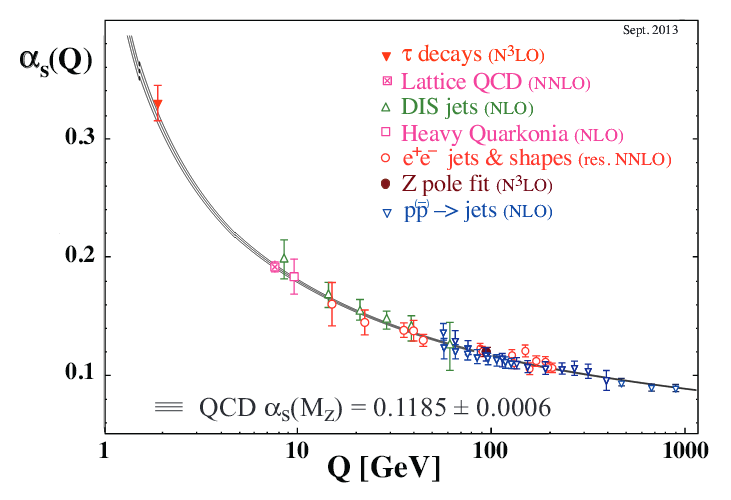
\includegraphics[width=1.0\linewidth]{figs/alphasrunning.png}
\caption{The QCD coupling constant $\alpha_{\mathrm{S}}$ as a function of the energy scale Q.}
\label{figs:alphasrunning}
\end{center}
\end{figure}
%from pdg


When a quark pair is produced with a high momentum, their separation increases quickly.  
As the separation of these quarks increases, the energy of the QCD field between them increases as well.  
If this separation is high enough, the energy between the quarks will reach a threshold where quark pair production is energetically favorable.  
At this threshold, the constituent quarks are then joined by these pair produced quarks.  
Additional quark pairs can be created many times, and the initial quark is detected as many hadrons that are collimated into a stream of particles called a jet.  
This process is called hadronization, 

The $\alpha_s$ parameter is low at short distances (or equivalently high energy); 
just like in QED, the impact of higher order diagrams is low.  
This allows the calculation of QCD diagrams using a finite perturbative expansion, and allows us to only consider only free quarks in high energy QCD calculations. 
The characteristic interaction energy where free quarks can be considered is around 400$\MeV$, which is much lower than energy scales 
considered in this thesis, so we will only be referring to free quark interactions.  


\section{The Weak Force}
\label{sec:weaktheory}
The weak force is felt by quarks and leptons alike.  
It is weaker than both the electromagnetic and the strong force, which leads to longer decay times for weakly decaying particles.  
The weak force is responsible for changing of quark flavor in an interaction.  
A vertex involving a change is quark flavor contributes a factor of $V_{ij}$ to the matrix element, where $V_{ij}$ is an element of the Cabibbo Kobayashi Maskawa (CKM) matrix 
(shown in Figure\ref{figs:CKM}).  
For example, the calculation of the diagram in Figure~\ref{figs:betaDecay} (beta decay) includes a factor of $V_{ud}$ = 0.97427.  
The CKM matrix is roughly diagonal, which means that a process which changes quark generation is rare.  

\begin{figure}
\begin{center}
\unitlength=1mm
\begin{fmffile}{feynman/betaDecay}
\begin{fmfgraph*}(40,30) \fmfpen{thick}
\fmfleft{i1,i2} \fmfright{sp1,sp2,sp3}
\fmf{phantom}{i2,v2,sp3}
\fmf{fermion}{i1,v1,sp1}
\fmf{fermion,tension=0.0}{v2,sp2}
\fmf{fermion,tension=0.0}{sp3,v2}
\fmf{photon,label=$W^{-}$}{v1,v2}
\fmflabel{$d$}{i1}
\fmflabel{$u$}{sp1}
\fmflabel{$e^-$}{sp2}
\fmflabel{$\nu_{e}$}{sp3}
\end{fmfgraph*}
\end{fmffile}
\end{center}
\caption{Feynman diagram depicting beta decay via
the weak interaction.}
\label{figs:betaDecay}
\end{figure}


Weak force interactions are dependent on the chirality of the interacting particle.
Chirality for massless particles is dependent on the relative orientation of the momentum and spin axes.  
Particles with momentum and spin aligned are referred to as right-handed, and particles with the momentum 
axis opposite to spin are left-handed\footnote{This convention is reversed for anti-particles}.
For massive particles this concept is generalized such that right- and left-handed components of a wavefunction 
can be extracted by using the right-handed operator (1+$\gamma^5$)/2 and the left-handed operator (1-$\gamma^5$)/2.  
The W boson only interacts with left-handed fermions whereas the Z boson interacts with right- and left-handed fermions with differing strengths. 

\begin{figure}
\begin{center}
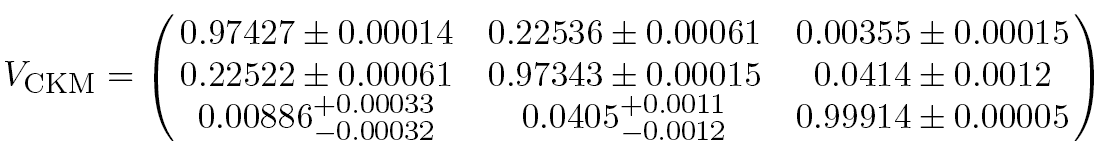
\includegraphics[width=1.0\linewidth]{figs/CKM.png}
\caption{The CKM quark mixing matrix.}
\label{figs:CKM}
\end{center}
\end{figure}



\section{Electroweak Symmetry Breaking}
%From pdg
Through the electroweak symmetry breaking mechanism, the mass of the W and Z bosons, and all fermions can be generated in the SM.  
We consider a scalar potenial of the form:
\begin{eqnarray}
\mathrm{ V(\Phi) = m^{2} \Phi^{\dagger} \Phi + \lambda ( \Phi^{\dagger} \Phi )^{2}  }\\
\mathrm{\Phi = \frac{1}{\sqrt{2}} \left( \frac{\sqrt{2} \phi^{+}}{\phi^{0} + ia^{0}}  \right)}
\end{eqnarray}  
where $\Phi$ is the Higgs field.  A plot of this potential can be seen in Figure~\ref{figs:higgspotential}.  
The minimum of the potential is not at V(0), and this point is unstable.  
The Higgs field has a non-zero vacuum expectation value (VEV).

\begin{figure}
\begin{center}
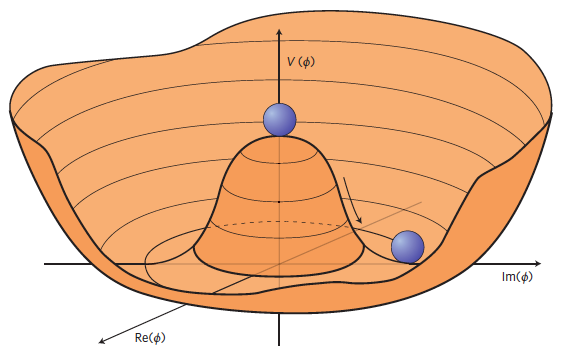
\includegraphics[width=0.7\linewidth]{figs/higgspotential.png}
\caption{The Higgs potential..}
\label{figs:higgspotential}
\end{center}
\end{figure}

Using the Higgs Lagrangian
\begin{eqnarray}
\mathrm{\cal(L) = (D_{\mu} \Phi )^{\dagger}(D_{\mu} \Phi ) -V( \Phi )}\\
(D_{\mu}\Phi) = (\partial_{\mu}+i g \sigma^{\alpha} W_{\mu}^{\alpha}/2 +i g^{'} Y B_{\mu}/2)\Phi
\end{eqnarray}  
we can extract the masses of the W and Z bosons as

\begin{eqnarray}
M_{W}^2 = \frac{g^{2}v^{2}}{4}\\
M_{Z}^2 = \frac{(g^{'2}+g^{2})v^{2}}{4}
\end{eqnarray}  

One new particle is predicted, a massive chargeless spin 0 particle called the Higgs boson.  
A particle consistent with the Higgs boson has been discovered in 2012 at the LHC.  
%https://cds.cern.ch/record/1638469/plots

  
\section{Beyond the Standard Model}
The SM is possibly the most successful theory in physics, but also one that is ultimately incomplete.  
We know that there are physical phenomena that the SM does not predict.  
The presence of dark matter and dark energy in the universe~\cite{Bennett:2003ba} is not currently explained by the SM.  
Given that dark matter and energy account for approximately 95\% of the universe, this is not a small issue.  
The SM does not explain the observation of neutrino oscillations~\cite{An:2012eh}, which implies that neutrinos have mass.  
The SM also does not naturally explain the relative values of fundamental constants such as why the weak force is $10^{33}$ times as strong as gravity.  
This issue is known as the hierarchy problem, and it is assumed that a complete theory would have a natural explanation for the seemingly random values of these constants.  

It is essential for a complete understanding of the universe that we probe beyond the standard model (BSM) theories that provide solutions to these issues.  
Theories involving compact extra dimensions~\cite{PhysRevD.64.035002} for example provide a natural explanation to the hierarchy problem.  
In these theories forces propegate in higher dimensions that are compactified.   
In this theory, the propagation of SM massive fields in higher dimensions leads to discrete modes, which are detectable as new massive particles.  
The propagation of the SM W or Z leads to excited modes that are referred to as the $\wpr$ and $\zpr$.
A novel way to look for BSM physics then is to attempt the creation and detection of massive states such as these bosons. 
In this thesis we discuss one such search for a W' boson.  

The W' boson is a particle predicted by many BSM theories such as Little Higgs~\cite{doi:10.1146/annurev.nucl.55.090704.151502}, 
Composite Higgs models~\cite{Vecchi:2013bja}, and Noncommuting Extended Technicolor~\cite{Chivukula:1995gu}.  





\chapter{Experimental Setup}
\label{sec:ExpSetup}
\chaptermark{Experimental Setup}
One way to search for BSM physics is to produce new particles directly.  
For this, we collide lighter particles at a high energy.  
The energy released in the collision can manifest in more massive particles\footnote{In SUSY there will usually be two} via mass-energy equivalence (E=m$\mathrm{c^2}$).
The collision may create one or more of these new particles, and from it's decay products an experimenter can reconstruct the properties of the new BSM massive state 
and study the properties (mass, decay width, spin, SM couplings etc.).  

For the measurements presented in this thesis, we collide high energy proton beams,  
which are designed to produce a high collision energy in comparison to fixed-target or electron-positron collisions.    
   
\section{Luminosity and Cross Section}
\label{sec:LumiXsec}
To understand how many occurrences of any physical process to expect in a set of collisions, we need to define at a minimum the concepts of luminosity, L, and cross section, $\sigma$.

The cross section of a process is a measure of the probability that a collision will produce the particles of interest.  
The phrase cross section refers to the physical cross section of a classical target and is thus measured in units of area.  
In a high energy collision, the cross section no longer refers to the physical dimensions of the target, and can be calculated directly from Feynman diagrams.  
The areas associated with these cross sections is very small and is measured in barns (b), which is $10^{-28} m^2$.  
BSM physics signatures have cross sections that are generally on the order of picobarns (pb) or femptobarns (fb).  
The process cross section is highly dependent of the energy of the collision and is why it is very important to have large, high energy accelerators for the discovery of new physics.  
The cross section of some SM processes are shown in Figure \ref{figs:SMxsecs}.


\begin{figure}
\begin{center}
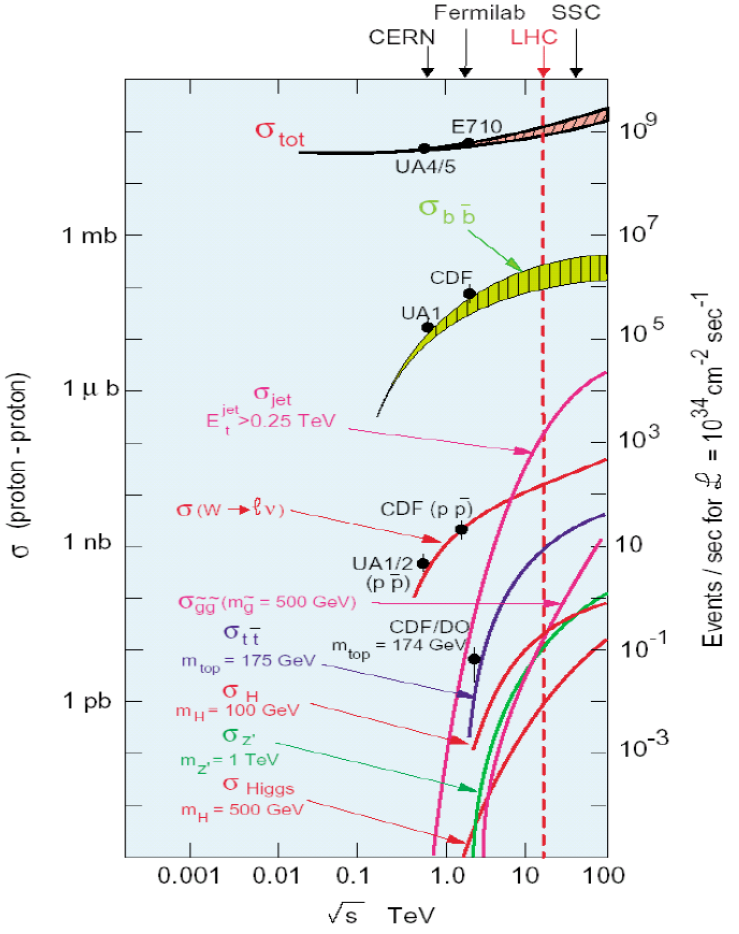
\includegraphics[width=0.7\linewidth]{figs/SMxsecs.png}
\caption{Standard model cross sections as a function of collision energy.}
\label{figs:SMxsecs}
\end{center}
\end{figure}


  
Luminosity is a measure of the intensity of the colliding beams and is the number of collisions expected per unit time per unit area.  
To look for BSM physics, we need to collect an ensemble of useful collisions (events), and thus higher luminosity leads to a larger 
ensemble, and consequently higher statistical precision of the measurement .  
Additionally, collecting data over time leads to a larger ensemble, so the time-integrated luminosity is a more useful variable to describe the total amount of data collected, 
which is reported in $\fbinv$.  Given in relevant collider properties, the luminosity can be defined as~\cite{Bayatian:922757}: 
\begin{eqnarray}
\mathrm{L = \frac{\gamma f k_{B} N_{p}^{2}}{4 \pi \epsilon \beta^{*}} F}
\end{eqnarray}  
where $\gamma$ is the Lorentz factor,  f is the frequency of revolution, $k_{B}$ is the number of bunches in the beam, $N_{p}$ is the number of protons per bunch, 
$\epsilon$ is the transverse emittance, $\beta^{*}$ is the betatron function, and F is a reduction factor based on the crossing angle.  

With these two concepts we can extract the predicted number of events, $N_{\mathrm{i}}$, for a given process i: 
\begin{eqnarray}
N_{\mathrm{i}} = \int L \mathrm{d}t \times \sigma_{\mathrm{i}} 
\label{eqn:Nevents}
\end{eqnarray}  

\section{The LHC}
The Large Hadron Collider (LHC) is a particle accelerator designed to reach collisions energies far surpassing any previous design.  
The LHC is a synchrotron that accelerates protons to 99.999997\% the speed of light.  
These protons beams are then collided at a center-of-mass energy ($\sqrt{s}$) of 8 $\TeV$.  
The accelerator segments and detectors at the LHC are shown in Figure~\ref{figs:lhc}.

% http://home.web.cern.ch/about/accelerators
% http://cds.cern.ch/record/1165534/files/CERN-Brochure-2009-003-Eng.pdf

A proton at the LHC starts out as hydrogen gas within the injector of LINAC 2 linear accelerator.  
The atoms are ionized using an electric field, stripping the electron.  
The resulting proton is accelerated using an oscillating electric field.  
The protons are accelerated in a straight line to an energy of 50~$\MeV$, or 31\% the speed of light.  

At this energy, linear acceleration is not practical, and the protons enter the Proton Synchrotron Booster (PSB).  The PSB is composed of four 157 m 
circumference superimposed synchrotrons that accelerate the protons using electric fields that are synchronized to the revolution frequency of the beams.  
The protons are kept on the circular accelerator with a magnetic field directed into the plane formed by the accelerator ring, which increases in strength as the protons gain energy.  
After the acceleration from the booster, the protons are at en energy of 1.4~$\GeV$, or 92\% the speed of light.

After the PSB, the protons enter the Proton Synchrotron (PS), a 628 m circumference synchrotron, which accelerates the protons to 25~$\GeV$, or 99.93\% the speed of light.  
After the PS, the protons enter the Super Proton Synchrotron (SPS), a 7 km circumference synchrotron, which accelerates the protons to 450~$\GeV$, or 99.9998\% the speed of light.

Finally, the beams enter the LHC.  This is the final synchrotron ring, with a circumference of 27 km.  
After the SPS, the protons are inserted into the LHC in one of two evacuated tunnels depending on which direction around the ring the beam is to travel.  

The LHC uses 1232 dipole magnets to keep the protons in the ring as they accelerate. which provide an 8.3 T field over their length.  
In order to deliver such a field, the magnets use superconducting niobium-titanium cables.  
These cables are cooled by superfluid helium to -271.3 C in order to achieve this superconductivity.  
During each revolution the energy of each proton in the LHC ring increases by 5 MeV.  
After being fully accelerated in the LHC, the protons are at an energy of 4~$\TeV$, or 99.999997 \%the speed of light.

The proton beams are then directed together for collisions in four positions around the ring.  
Each beam in the LHC ring contains 2808 bunches of protons, and each bunch contains 110 billion protons. 
These bunches need to be collimated in order to maximize collision frequency, which is accomplished by the use of 392 focusing quadrupole magnets.   
Each of these collision points houses its own detector, ALICE (A Large Ion Collider Experiment), ATLAS (A Toroidal LHC Apparatus), 
CMS (Compact Muon Solenoid), and LHCb (Large Hadron Collider beauty).  
The ALICE detector is primarily used for experiments involving heavy ion collisions that expand the current 
understanding of concepts such as the quark-gluon plasma and quark confinement   
LHCb is specialized for physics involving b quarks, such as measuring CP violation parameters from b-hadron interactions.  

CMS and ATLAS are large general purpose detectors.  
These detectors are used for many different types of physics searches, and are the two detectors responsible for the Higgs boson discovery.  
For the purposes of this thesis we will be concentrating on the CMS detector
  


\begin{figure}
\begin{center}
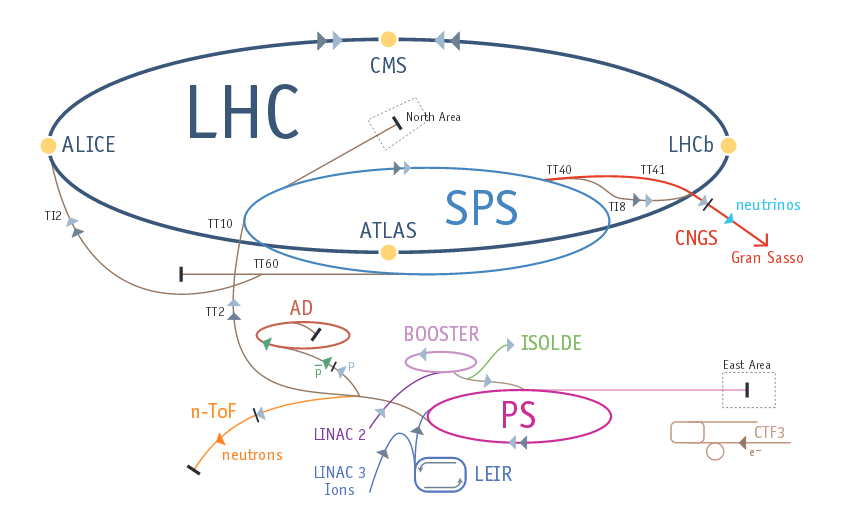
\includegraphics[width=1.0\linewidth]{figs/lhc.png}
\caption{A diagram of the LHC~\cite{lhcbrochure}.}
\label{figs:lhc}
\end{center}
\end{figure}
%http://cds.cern.ch/record/1092437/files/CERN-Brochure-2008-001-Eng.pdf

\section{CMS detector}
Here we will detail the basics of the CMS detector subsystems, for a more complete description, see Reference \cite{Bayatian:922757}.
The purpose of the CMS detector is to measure properties of particles that are created in a collision such as the energy and trajectory. 
The detector needs to collect enough information so that particles can be reconstructed and classified.  
Generally, we can reconstruct most physics signatures by analyzing electrons, muons, photon, charged hadrons, and neutral hadrons. 
The CMS detector has dedicated algorithms and systems that are specifically designed to identify each of these categories.  In order to reconstruct these particles, we impose a uniform axial magnetic field throughout the inner detector with the use of a superconducting magnet. 

The trajectory of charged particles is important for extracting information such as charge and momentum.  
The process of reconstructing the trajectory of these  particles is called tracking.  
Near the interaction point tracks are very dense, and tracking becomes very difficult.  
In this region we use a fine array of silicon pixels that register a charge particles position based on charge deposited in the device.  
Additional measurements are made by a second series of silicon detectors called the Silicon Strip Tracker. 
Using a series of these position measurements, we can fit a charged particle track.  

Energy can be measured by the use of calorimeter systems.  
A calorimeter is a detector designed such that a particle will deposit all of its energy within its volume in the form of photons, 
which can be detected to extract a measure of the total energy. 
These systems are subdivided into the Electromagnetic Calorimeter (ECAL) and Hadronic Calorimeter (HCAL).  
The ECAL uses scintillation crystals to detect particles that interact primarily with the electromagnetic force such as electrons and photons.  
Hadrons pass through the ECAL with minimal loss and deposit energy in the HCAL, which uses layers of absorber and scintillator to first 
create a shower of secondary particles, and then measure the total energy of these secondary particles.  

The detection of muons requires a specially designed system that lies outside of the ECAL, HCAL, and magnet.  
Muons pass through the ECAL and HCAL without losing a substantial fraction of their energy.  
To reconstruct the trajectory of muons, we use several different systems both inside and outside the magnet.

See Figure~\ref{figs:CMSdiagram1} for a diagram of the full detector, and Figure~\ref{figs:CMSdiagram} for a cross-sectional view of the detector subsystems.

\begin{figure}
\begin{center}
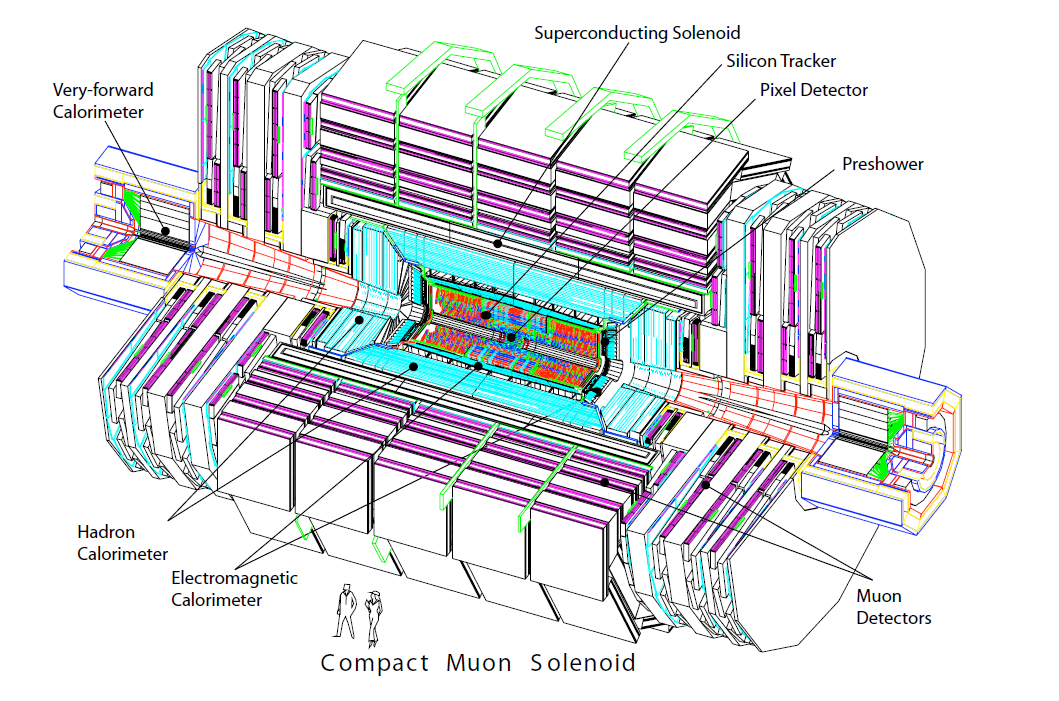
\includegraphics[width=1.0\linewidth]{figs/CMSdiagram1.png}
\caption{A diagram of the full CMS detector.}
\label{figs:CMSdiagram1}
\end{center}
\end{figure}

\begin{figure}
\begin{center}
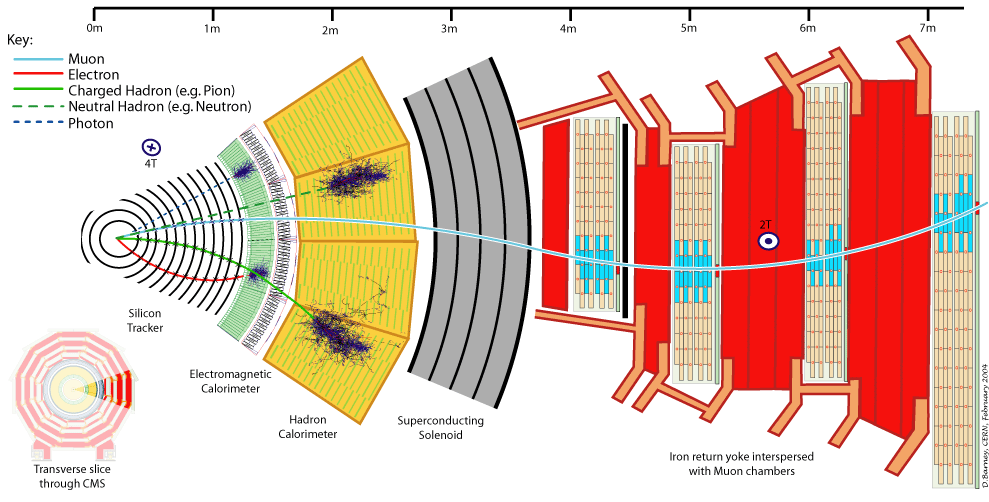
\includegraphics[width=1.0\linewidth]{figs/CMSdiagram.png}
\caption{A cross-sectional view of the CMS detector.}
\label{figs:CMSdiagram}
\end{center}
\end{figure}



\subsection{Pixel Tracker}
The closest detector system to the interaction point is the silicon pixel tracking system (see Figure \ref{figs:CMSpixel}).   .  
This system extends from a radius of 4 cm to 11 cm in the barrel, and is designed to track charged particles in a very dense environment.  
This is achieved with three arrays of two dimensional silicon pixels placed at a radii of 4.4 cm, 7.3 cm, and 10.2 cm, as well as two endcap disks for a total of 65 million pixels.  
When a charged particle traverses one of the 100 $\mum$ $\times$ 150 $\mum$ pixels, it imparts enough energy to the silicon to eject an electron.  
The electrons and their corresponding hole are detected on the pixel surface as a signal.  
This signal allows us to extract a position measurement for the charged particle.  

The entire system exists in a magnetic field, so the trajectory of the electrons and holes are deflected in the r,$\phi$ plane before detection.  
The angle of this Lorentz drift is 23$\textdegrees$, which causes the electron-hole pairs to be detected over a wide region covering multiple pixels.  
This effect improves the spacial resolution to 10 $\mum$ in r-$\phi$ space due to the fact that the charge center can be reconstructed by more measurements, 
whereas the z resolution is 20 $\mum$ due to the fact that there is no magnetic deflection in this direction. 
The pixel detectors in the endcap disks are angled at 20$\textdegrees$ in a turbine-like design to take advantage of this effect.  

  

\begin{figure}
\begin{center}
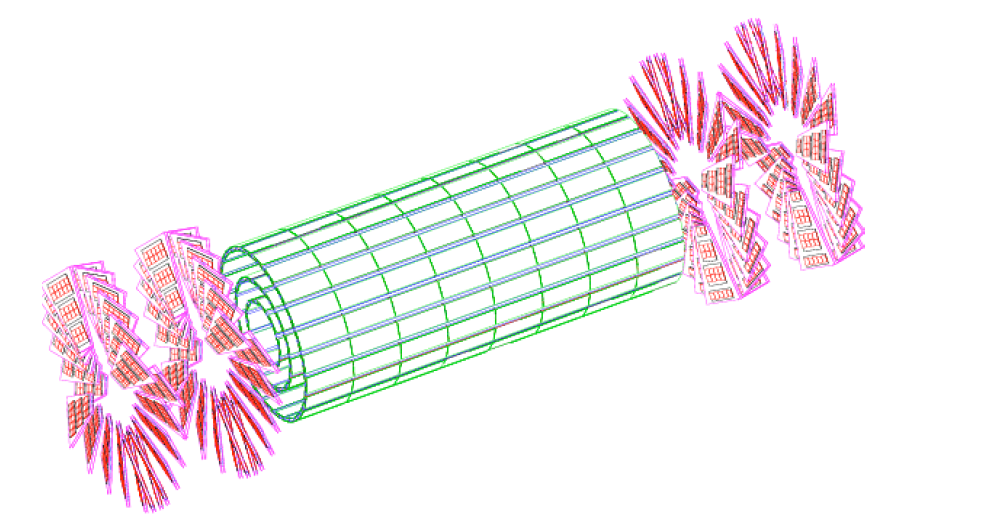
\includegraphics[width=1.0\linewidth]{figs/CMSpixel.png}
\caption{A diagram of the pixel detector.}
\label{figs:CMSpixel}
\end{center}
\end{figure}
  
\subsection{Silicon Strip Tracker}
Outside of the silicon pixel tracker (see Figure \ref{figs:CMStracker}) out to a radius of 130 cm in the barrel lies the silicon strip tracking system.  

The system in segmented into the inner barrel, outer barrel, inner disk, and endcap segments.  
The inner barrel segment (20 cm $<$ r $<$ 55 cm) uses four arrays of 10 cm $\times$ 80 $\mum$ silicon microstrips .  
The outer barrel (55 cm  $<$ r $<$ 130 cm) uses six arrays of large pitch 25 cm $\times$ 180 $\mum$ silicon microstrips.  

The endcap silicon strip detector consists of nine disks from 120 cm  $<$ z $<$ 280 cm.  
The inner disk segment contains three smaller disks that connect the inner barrel and endcap segments.  

\begin{figure}
\begin{center}
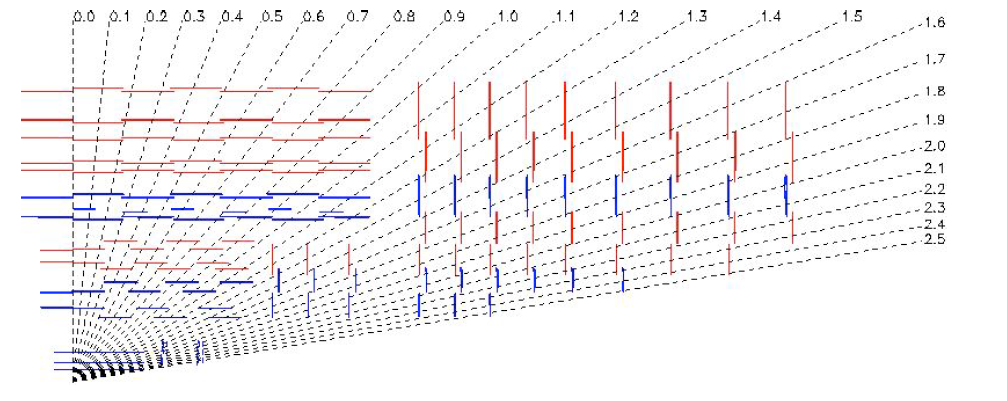
\includegraphics[width=1.0\linewidth]{figs/CMStracker.png}
\caption{A diagram of the silicon tracking system.}
\label{figs:CMStracker}
\end{center}
\end{figure}
  


%\subsection{Preshower Calorimeter}
\subsection{Electromagnetic Calorimeter}
The ECAL (see Figure~\ref{figs:CMSecal}) is designed to provide energy information for electrons and photons.  
These particles will typically deposit all of their energy within the detector, which is detectable as photons. 

To do this, the ECAL uses 61200 lead tungstate ($\mathrm{PbWO_4}$) scintillation crystals in the barrel and 7324 in each endcap.  
Lead tungstate is chosen as a scintillation material because it has a short radiation length (0.89 cm), fast response (25 ns for 80\% of light), and can 
withstand harsh radiation environments (10 Mrad).
The light emitted is around 30 photons per $\MeV$ for the energy of the particle of interest, which is somewhat low.  
Therefore, the ECAL uses avalanche photodiodes in the barrel and voltage phototriodes in the endcap segments to amplify the signal upon readout.  

The endcap regions of the ECAL include a preshower detector that is used to distinguish high energy photons from decaying pions.  
A pion decaying to two closely spaced photons can mimic one high energy photon to the 2.2 cm wide ECAL crystals.  
The preshower is able to distinguish these events with a finer granularity (2 mm) silicon strip detector.   
 
\begin{figure}
\begin{center}
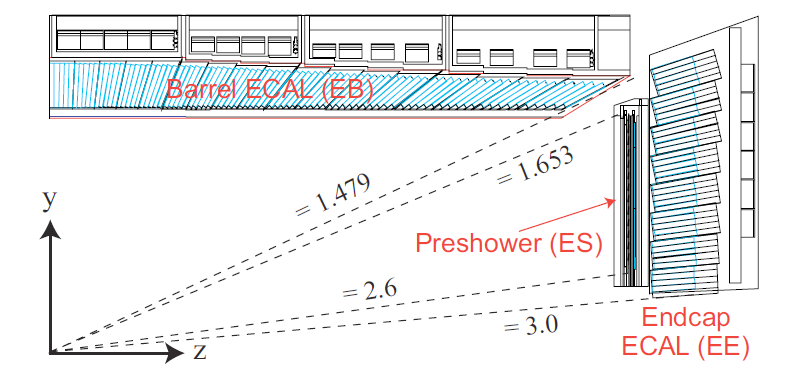
\includegraphics[width=1.0\linewidth]{figs/CMSecal.png}
\caption{A diagram of the ECAL system.}
\label{figs:CMSecal}
\end{center}
\end{figure}
  





\subsection{Hadronic Calorimeter}
The HCAL (see Figure~\ref{figs:CMShcal}) is designed to give the energy of charged and neutral hadrons, which generally lose very little energy in the ECAL.  
The HCAL is segmented into the inner barrel (inside the magnet), outer barrel (outside the magnet), endcap, and forward (close to the beamline).  

The HCAL uses alternating layers of absorber and scintillator to calculate the energy of these hadrons.  
The absorber creates a cascade of secondary particles that emit photons in the scintillator which can then be detected and summed to reconstruct the energy of the initial hadron.  
The photons emitted in the scintillator are carried to the photodetectors by optical waveguides.  
The HCAL uses hybrid photodiodes to detect the scintillation light and provide a signal that can be used to extract the total energy of the hadron.  

\begin{figure}
\begin{center}
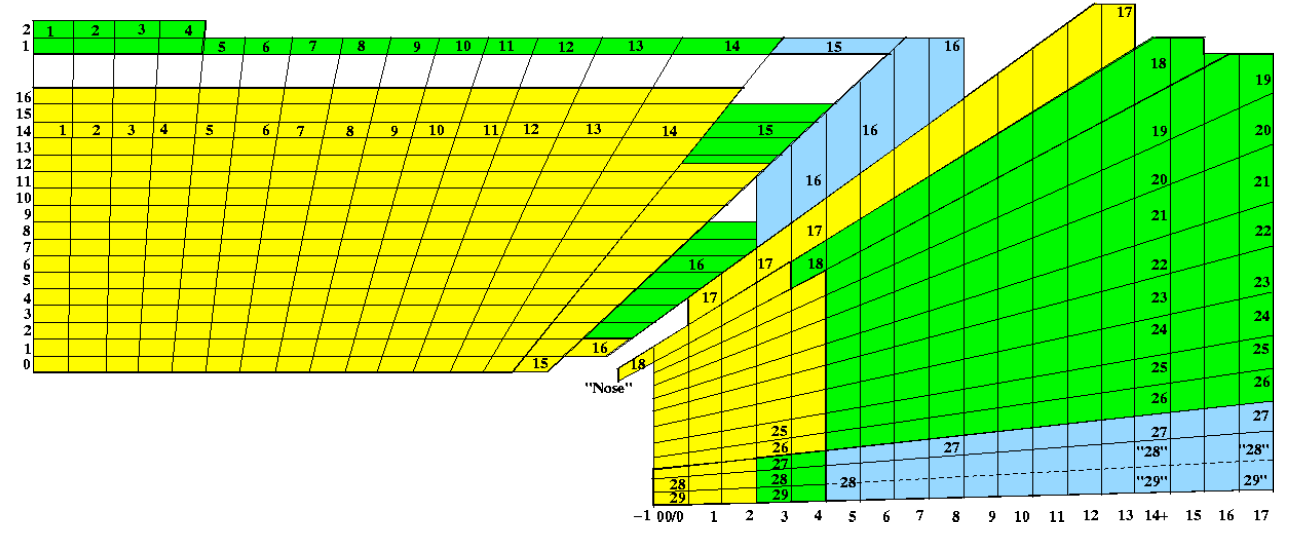
\includegraphics[width=1.0\linewidth]{figs/CMShcal.png}
\caption{A diagram of the HCAL system.}
\label{figs:CMShcal}
\end{center}
\end{figure}
  
\subsection{Magnet}
A charged particle moving perpendicular to a magnetic field follows a helical trajectory.  
The curvature of this helix is dependent on the momentum of the particle, and the handedness is dependent on the charge.  
Therefore, by immersing the tracking volume in an axial magnetic field we can get an accurate measurement of these properties.  
The stronger the magnetic field, the more precise these measurements can be for a high energy particle due to the more distinct curvature.  
To produce this field, CMS employs the largest superconducting magnet ever built.  

The design goal for the magnet is to be able to reproduce high momentum muons.  
The benchmark used for this is to have a momentum resolution of $\Delta$p/p $\leq$ 10\% at a muon momentum of 1 $\TeV$.  
To achieve this, we employ a solenoid with a length of 12.9 m and bore of 5.9 m.  
The coils of this solenoid are superconducting niobium-titanium, which produce a uniform 3.8 T magnetic field in the interior. 
The coils are wound in four layers, for a total of 2168 turns that carry 19.5 kA of current.    

The magnet additionally provides structural support to withstand the weight of the CMS detector as well as the magnetic force exerted from it's own magnetic field.  

\subsection{Muon System}
The reconstruction of muons and electrons starts at the inner silicon tracking system.  
Whereas electrons deposit their energy in the ECAL, a muon will traverse the ECAL and HCAL without significant interaction because a muon is around 200 times as massive.  
Muons are of interest to the Higgs discovery as well as BSM physics, 
and an accurate determination of the muon energy is also required for determination of the total event energy and missing energy.  
Therefore, the CMS detector has a large system purely designed to reconstruct muons, which lies outside all other detector systems at CMS.  

The muon system is comprised of a gaseous detectors interleaved with iron.  
The iron is saturated with the return field of the magnet, which creates a magnetic field at one half of the internal field strength and oriented in the opposite direction.  
The three layers of this ``return yoke" system bends muons to get an accurate measure of the momentum outside of the magnet.  

The trajectory of the muons is reconstructed with three types of gaseous detectors.  
The detectors work on the same basic principle, where an incoming muon ionizes the gas creating an electron-hole pair.  
The electron is detected by the anode, and the hole is detected by a cathode.  
A coincidence of these two measurements gives a measure of the position and time that a muon traversed the detector.  
With a series of these measurements, a trajectory can be fit, and physical quantities of interest can be reconstructed.  

In the barrel region ($|\eta|$ $<$ 1.2), drift tubes are used because the neutron flux and magnetic field are low.  
A drift tube is a detector consisting of a gas filled tube with an anode wire.  
The ionized electron from the gas volume travels to the anode wire, and a measurement of position is made.  
The detection of this electron registers the position along the wire (z coordinate).  
The r-$\phi$ coordinate within the drift tube cross sectional can be calculated by using the drift time of the ionized electrons to the anode.  

In the endcap region, where the magnetic field and neutron flux are high, cathode strip chambers are used.  
Cathode strip chambers are trapezoidal in shape with six gas gaps for ionization.  
These gas gaps each have one plane of cathode strips pointing radially outward and one plane of anode wires oriented perpendicular to the cathode.  

In both the barrel and endcap regions, resistive plate chambers are used.  
These detectors are composed of two parallel resistive plates separated by a gas gap.  
The design goal of the resistive plate chambers is to complement the cathode strip chambers and drift tubes to give two independent measurements of position.  
Additionally, resistive plate chambers offer very quick and accurate time resolution.  This offers a 
quick approximation of the muon momentum which is useful for the trigger system and matching a muon track to a bunch crossing.  

The muon system and inner tracker both contribute to the trajectory measurement of a muon.  
In terms of momentum resolution, the inner tracker offers much better sensitivity up to around 200 $\GeV$.  
After 200 $\GeV$, the muon system starts to significantly improve the momentum measurement.

Figure \ref{figs:CMSmuon} shows a diagram of the muon system.  
\begin{figure}
\begin{center}
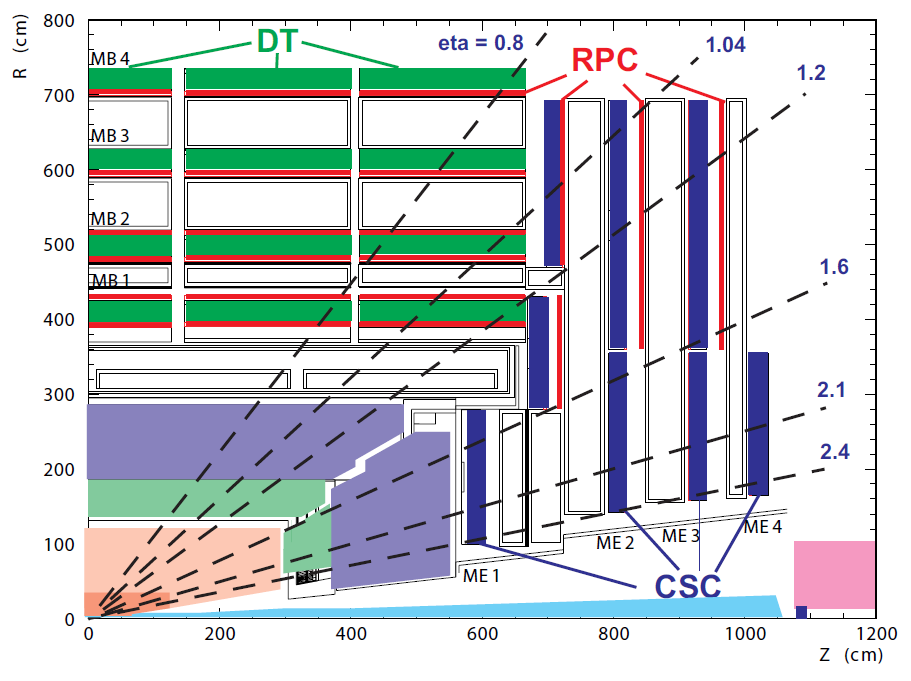
\includegraphics[width=1.0\linewidth]{figs/CMSmuon.png}
\caption{A diagram of the muon system.}
\label{figs:CMSmuon}
\end{center}
\end{figure}

\subsection{Trigger}
The LHC delivers around 1 billion proton-proton collisions per second.  
However, because of the current computing limitations, the CMS detector system can only write around 100 collisions per second as data.  
Therefore, a trigger system is developed to distinguish the most potentially interesting physics signatures.  

The L1 trigger takes information from the calorimeter and muon systems and their correlations.  
When one of these detectors produces a signal, the information takes 3.2 $\mus$ to reach the L1 processing area and return to the detector.  
The L1 processing time for the information for a maximum of 1 $\mus$ where the decision is made to keep the event to search for potential physics signatures.  
The L1 has various algorithms designed to keep ``trigger primitives", which can be objects such as high $\pt$ muons, electrons, jets or full event information like total energy or $\MET$.  
The L1 trigger only saves on average of 1 out of every 1000 events.  

After the L1 trigger, the trigger primitive events are processed by the high level trigger (HLT).  
The HLT again saves only 1 out of 1000 of these events.  
The processing time for the HLT algorithm is longer than the L1 system, and to extract the potentially exciting physics objects the algorithm performs partial event reconstruction.  
An event that enters the HLT algorithm is first analyzed based on the output of the calorimeters and muon system, then pixel tracking is performed, then finally full tracking.  
An event that passes the L1 and HLT is then put into storage for analysis.  

%\subsection{Computing Grid}




\chapter{Introduction to the $\wpr$ Search}

\label{sec:introduction}

Many beyond the Standard Model (BSM) theories predict new massive
gauge bosons.  This note presents a search for a heavy partner of
the Standard Model (SM) W gauge boson, generally referred to as the
$\wpr$ (see Chapter~\ref{sec:BSMtheory}).  
We focus on the $\wpr \to \tbbar$ decay mode motivated by the ability to lower QCD multijet background in this channel when compared to light flavor hadronic decay modes. 


The primary signal under investigation is a $\wpr$ particle in which the interaction with quarks 
is defined by the following Lagrangian,
\begin{eqnarray}
{\cal L} = \frac{V_{q_iq_j}}{2\sqrt{2}} g_w \overline{q}_i\gamma_\mu 
\bigl( a^R_{q_iq_j} (1+{\gamma}^5) + a^L_{q_iq_j}
(1-{\gamma}^5)\bigr) {\wpr} q_j + \mathrm{H.c.} \,,
\label{eqn:Lag}
\end{eqnarray}
This is the most general, lowest-dimensional, model-independent
effective Lagrangian for the $\wpr$ boson.  Here $a_{qi,qj}^{L}$,
$a_{qi,qj}^{R}$ are the left- and right-handed couplings of $\wpr$ to quarks.
For a SM-like $\wpr$, $a_{qi,qj}^{L}$=1, $a_{qi,qj}^{R}=0$.


Searches for a high mass $\wpr$ resonance have been performed at the
Tevatron \cite{PhysRevLett.100.211803,Abazov2011145} and at CMS \cite{CMS-PAS-B2G-12-010,CMS-PAS-EXO-12-060,CMS-PAS-EXO-12-025} and ATLAS \cite{PhysRevLett.109.081801} at the LHC.  
Currently, the most stringent limits on $\wpr$ cross-sections exclude a right-handed $\wpr$ particle with mass below 2.05$~\TeV$ at the 95\% C.L. In this analysis we do not consider \wpr\
  lighter than $\sim$~1.3~$\TeV$ since there are stringent limits on $\wpr$ production at these masses.  

We present a search for $\wpr \to \tbbar$ followed by the
fully hadronic decay chain $\mathrm{t \to W+b}$ followed by $\mathrm{W \to hadrons}$.
This differs from \cite{CMS-PAS-B2G-12-010} since the final state is
comprised of only jets.  In our kinematic regime of interest ($\mathrm{M_{\wpr}
\gtrsim 1.3~\TeV}$) the top quark is quite energetic, and due to its Lorentz
boost, the angular separation between its immediate decay products will
be small.  The jets resulting from the hadronization of the b quark
and the light quarks from W boson from the top decay usually overlap, resulting in one
`fat' jet.  This search uses special techniques to identify the
substructure of this top jet, and further selection based on
substructure information as well as b-tagging strongly suppresses the
QCD background.

The search uses $19.7~\fbinv$ of 8$~\TeV$ data collected from
the CMS experiment in 2012.


\chapter{Analysis Strategy}
\label{sec:analysisStrategy}

%The primary focus of this analysis is a high mass resonance ($>1.3$~\TeV) decaying to $\tbbar$. At higher energies, the top decay products merge into a single jet. We 
%consider the case of a top decaying in the fully hadronic decay chain $t \to W+b$ followed by $W \to$ hadrons. These high energy final states lead to an inefficient 
%determination of the limits on production of $M_{\wpr}$ with masses below  $1.3~\TeV$, which are not included in the analysis.  

The focus of this analysis are heavy resonances decaying into
$\tbbar$.  Thus the $\wpr \to \tbbar$ decay results in a mostly
dijet topology, with the b and top jets being  predominantly back-to-back. 
% Events that have this topology are referred to as ``type
% b+1'' referring to the completely merged top candidate as a ``type 1''
% top and the b candidate jet in the opposite hemisphere.  
% The event topology
% is similar to reference \cite{7tevZprime}, however this analysis does
% not include the ``type 1+2'' topology, due to the negligible signal
% efficiency in the kinematic region of interest.  The type b+1 analysis
% is then a dijet search (one jet in each hemisphere).

After requiring a high transverse momentum, 
the primary sources of background are QCD multijet and SM $\ttbar$ 
production due to the high abundance of QCD present by requiring a dijet topology and the high $\ttbar$ production contribution fraction that remains after top jet discrimination. 

Of these two main sources, QCD multijet production is dominant and is estimated by a data driven technique similar 
to \cite{7tevZprime}.  We
invert certain substructure cuts used to identify top jets
to define sideband regions; we keep the cut on the mass of the
top jet to avoid the kinematic bias in forming the invariant mass
distribution of the top-b candidate.  One sideband region is used
to measure the average b-tagging rate, which is then applied to
pre-b-tag data to obtain the QCD estimate.  The other sidebands are
then used to check the performance of the QCD estimation in data.

The SM $\ttbar$ contribution is estimated from Monte Carlo (MC) simulation.
We also subtract the pre-tagged $\ttbar$ from the pre-tagged data sample when
measuring the average b-tagging rate.  The measurement
of the average b-tagging rate is then independent of $\ttbar$, and the 
$\ttbar$ contribution is added at the end as a separate background
component.
The contribution of the single top production to the background was
found to be negligible.

% &&& need to put the study proving this into the appendix

The data and background components are then used as
templates by the Bayesian statistical procedure 
to set the exclusion limits on $\wpr$.  This procedure uses a binned likelihood to calculate limits for the signal cross-section 
in the $\wpr \to \tbbar$ branching fraction.  
We use the limit setting framework ``Theta'' \cite{theta}, which calculates exclusion limits using a shape based approach.

\chapter{Data Sample and Event Selection}
\label{sec:datasampleAndSelection}
The data sample used for this analysis corresponds to 19.7$\pm0.5~\fbinv$ of integrated 
luminosity collected in 2012 at $\sqrt{s} = 8~\TeV$.  See Table \ref{table:datasets} for a summary of the datasets used in the analysis.
Generation of Standard Model $\ttbar$ and single top events is performed by Powheg.  The Monte Carlo simulation samples used for background estimation can be found in table \ref{table:datasets}.

\begin{table}
\begin{center}
\bf{Jet Datasets}
\begin{tabular}{|p{0.7\linewidth}|c|}
\hline
\bf{Dataset} & \bf{Luminosity ($\pbinv$)} \\
\hline
/Jet/Run2012A-22Jan2013-v1/AOD & $888$ \\
/JetHT/Run2012B-22Jan2013-v1/AOD & $4403$ \\
/JetHT/Run2012C-22Jan2013-v1/AOD & $7052$ \\
/JetHT/Run2012D-22Jan2013-v1/AOD & $7414$ \\
\hline
Total Analyzed Luminosity & $19757$ \\
\hline
\end{tabular}
\bf{Monte Carlo Datasets} \\
\begin{tabular}{|p{0.7\linewidth}|c|}
\hline
\bf{Dataset} & \bf{Cross-section(pb)} \\
\hline
TT\_Mtt-700to1000\_CT10\_TuneZ2star\_8TeV-powheg-tauola & $245.8$ (NNLO)\\
TT\_Mtt-1000toInf\_CT10\_TuneZ2star\_8TeV-powheg-tauola & $245.8$ (NNLO)\\
T\_t-channel\_TuneZ2star\_8TeV-powheg-tauola & $56.4$ (NNLO)\\
Tbar\_t-channel\_TuneZ2star\_8TeV-powheg-tauola & $30.7$ (NNLO)\\
Tbar\_tW-channel-DR\_TuneZ2star\_8TeV-powheg-tauola & $11.1$ (NNLO)\\
T\_tW-channel-DR\_TuneZ2star\_8TeV-powheg-tauola & $11.1$ (NNLO)\\
T\_s-channel\_TuneZ2star\_8TeV-powheg-tauola & $3.79$ (NNLO)\\
Tbar\_s-channel\_TuneZ2star\_8TeV-powheg-tauola & $1.76$ (NNLO)\\
QCD\_Pt-300to470\_TuneZ2star\_8TeV\_pythia6 & $1759.6$ \\
QCD\_Pt-470to600\_TuneZ2star\_8TeV\_pythia6 & $113.9$ \\
QCD\_Pt-600to800\_TuneZ2star\_8TeV\_pythia6 & $27.0$ \\
QCD\_Pt-800to1000\_TuneZ2star\_8TeV\_pythia6 & $3.57$ \\
QCD\_Pt-1000to1400\_TuneZ2star\_8TeV\_pythia6 & $0.738$ \\
QCD\_Pt-1400to1800\_TuneZ2star\_8TeV\_pythia6 & $0.0335$ \\
\hline

\end{tabular}
\end{center}
\caption{Primary datasets and Monte Carlo samples used. Including the corresponding integrated luminosity or cross-section of each dataset \cite{Czakon:2013goa,Kidonakis:2012db}.}
\label{table:datasets}
\end{table}

\section{Signal Samples}
\label{sec:signal}
The Lagrangian presented in equation \ref{eqn:Lag} has been implemented in CompHEP \cite{CompHEP} and used for event generation.  The mass of the top 
quark was set to 172.5~$\GeV$.  
Pythia was used for hadronization. The CTEQ6M parton distribution functions were selected and the QCD scale was set to the $\wpr$ invariant mass.  The width of 
the $\wpr$ resonance and cross-sections were obtained from CompHEP numerical calculations.  The generation was performed using the 2 $\rightarrow$ 4 
process $\wpr \rightarrow$ t ; t $\rightarrow$ Wb ; W $\rightarrow$ $q_{i}q_{j}$, where $q_{i}$ and $q_{j}$ represent quarks.  
W decays including b quarks are not considered due to the negligible branching fraction.  The process 
preserves all spin correlations between production and decay.

The $\wpr$ generation can be performed using three different couplings. 
\begin{itemize}
\item {\bf $\wpr_{R}$} - The purely right-handed $\wpr$ where $a_{qi,qj}^{L}$=0 , $a_{qi,qj}^{R}$=1 
\item {\bf $\wpr_{L}$} - The purely left-handed $\wpr$ where $a_{qi,qj}^{L}$=1 , $a_{qi,qj}^{R}$=0 
\item {\bf $\wpr_{LR}$} - The mixed-coupling $\wpr$ where $a_{qi,qj}^{L}$=1 , $a_{qi,qj}^{R}$=1 
\end{itemize}

Because of the SM-like couplings of $\wpr_{L}$ and $\wpr_{LR}$, we must consider the 
interference between SM single top and signal.  The $\wpr_{R}$ Monte Carlo samples were generated without SM single top.  The right-handed $\wpr$ samples used in this analysis are given in table
\ref{table:signalsets}.  The cross-sections listed here are leading order.  The cross-sections 
used in the main analysis are scaled to next-to leading order with a multiplicative k factor of 1.2
which is extracted from \cite{kfactor}.  The left-handed and mixed-coupling $\wpr$ samples used 
in this analysis are given in table \ref{table:signalsetsleft} and \ref{table:signalsetsmixed} respectively.
In order to have sufficient statistical precision in the signal region, these samples have a loose generator 
level $\pt$ cut of 200$~\GeV$ set on the b jet from the $\wpr$ decay.  The effect of this pre-selection is investigated in section \ref{sec:GenBptCut}.

\begin{table}
\begin{center}
\bf{Right-Handed Signal Samples}
\begin{tabular}{|p{0.46\linewidth}|c|c|}
\hline
\bf{Dataset} & \bf{$\Gamma_{\wpr} (\GeV)$} & \bf{(LO) Cross-Section (pb)} \\
\hline
SingletopWprimeTToHad\_M-1300\_right\_TuneZ2star\_8TeV-comphep & 43.7 & 0.4852 \\
\hline
SingletopWprimeTToHad\_M-1500\_right\_TuneZ2star\_8TeV-comphep  & 50.0 & 0.2198 \\
\hline
SingletopWprimeTToHad\_M-1700\_right\_TuneZ2star\_8TeV-comphep  & 57.3 & 0.1038 \\
\hline
SingletopWprimeTToHad\_M-1900\_right\_TuneZ2star\_8TeV-comphep  & 64.1 & 0.0507 \\
\hline
SingletopWprimeTToHad\_M-2100\_right\_TuneZ2star\_8TeV-comphep  & 70.9 & 0.0254 \\
\hline
SingletopWprimeTToHad\_M-2300\_right\_TuneZ2star\_8TeV-comphep  & 77.6 & 0.0131 \\
\hline
SingletopWprimeTToHad\_M-2700\_right\_TuneZ2star\_8TeV-comphep  & 91.2 & 0.0039 \\
\hline
\end{tabular}
\end{center}
\caption{Signal samples used in the analysis.  Quoted cross-section and $\Gamma_{\wpr}$ were obtained from the CompHEP generator. A k factor of 1.2 is implemented on the quoted cross-sections.}
\label{table:signalsets}
\end{table}


\begin{table}
\begin{center}
\bf{Left-Handed Signal Samples}
\scalebox{0.75}{
\begin{tabular}{|p{0.46\linewidth}|c|c|c|}
\hline
\bf{Dataset} & \bf{$\Gamma_{\wpr} (\GeV)$} & \bf{(LO) Cross-Section (pb)} & \bf{Selection Efficiency} \\
\hline
SingletopWprimeTToHad\_M-1300\_left\_TuneZ2star\_8TeV-comphep & 43.7 & 0.4248 & 0.157 \\
\hline
SingletopWprimeTToHad\_M-1500\_left\_TuneZ2star\_8TeV-comphep  & 50.0 & 0.2622 & 0.104 \\
\hline
SingletopWprimeTToHad\_M-1700\_left\_TuneZ2star\_8TeV-comphep  & 57.3 & 0.1669 & 0.0679 \\
\hline
SingletopWprimeTToHad\_M-1900\_left\_TuneZ2star\_8TeV-comphep  & 64.1 & 0.1237 & 0.0507 \\
\hline
SingletopWprimeTToHad\_M-2100\_left\_TuneZ2star\_8TeV-comphep  & 70.9 & 0.1047 & 0.0429 \\
\hline
SingletopWprimeTToHad\_M-2300\_left\_TuneZ2star\_8TeV-comphep  & 77.6 & 0.0971 & 0.0397 \\
\hline
SingletopWprimeTToHad\_M-2700\_left\_TuneZ2star\_8TeV-comphep  & 91.2 & 0.0933 & 0.0379 \\
\hline
\end{tabular}
}
\end{center}
\caption{Left-Handed signal samples used in the analysis.  Quoted cross-section and $\Gamma_{\wpr}$ were obtained from the CompHEP generator.  A k factor of 1.2 is implemented on the quoted cross-sections.  The cross sections listed here take into account the generator level b jet $\pt$ cut, and represent the visible cross section.  The efficiency of this cut is provided under the column labeled Selection Efficiency.}
\label{table:signalsetsleft}
\end{table}

\begin{table}
\begin{center}
\bf{Mixed Signal Samples}
\scalebox{0.75}{
\begin{tabular}{|p{0.46\linewidth}|c|c|c|}
\hline
\bf{Dataset} & \bf{$\Gamma_{\wpr} (\GeV)$} & \bf{(LO) Cross-Section (pb)} & \bf{Selection Efficiency} \\
\hline
SingletopWprimeTToHad\_M-1300\_mixed\_TuneZ2star\_8TeV-comphep & 87.4 & 0.9327 & 0.290 \\
\hline
SingletopWprimeTToHad\_M-1500\_mixed\_TuneZ2star\_8TeV-comphep & 101.0 & 0.4743 & 0.172 \\
\hline
SingletopWprimeTToHad\_M-1700\_mixed\_TuneZ2star\_8TeV-comphep & 114.6 & 0.2700 & 0.105 \\
\hline
SingletopWprimeTToHad\_M-1900\_mixed\_TuneZ2star\_8TeV-comphep & 128.2 & 0.1776 & 0.0711 \\
\hline
SingletopWprimeTToHad\_M-2100\_mixed\_TuneZ2star\_8TeV-comphep & 141.7 & 0.1334 & 0.0540 \\
\hline
SingletopWprimeTToHad\_M-2300\_mixed\_TuneZ2star\_8TeV-comphep & 155.3 & 0.1128 & 0.0458 \\
\hline
SingletopWprimeTToHad\_M-2700\_mixed\_TuneZ2star\_8TeV-comphep & 182.4 & 0.0986 & 0.0400 \\
\hline
\end{tabular}
}
\end{center}
\caption{Mixed-Coupling signal samples used in the analysis.  Quoted cross-section and $\Gamma_{\wpr}$ were obtained from the CompHEP generator.  A k factor of 1.2 is implemented on the quoted cross-sections.  The cross sections listed here take into account the generator level b jet $\pt$ cut, and represent the visible cross section.  The efficiency of this cut is provided under the column labeled Selection Efficiency.}
\label{table:signalsetsmixed}
\end{table}


\section{Trigger Selection}
\label{sec:trigger}
Due to our interest in highly boosted jets, our data was taken using the \texttt{HLT\_HT750} trigger, which requires the event to have $\mathrm{H_t}$ of at least 750 $\GeV$. 
The trigger efficiency is measured in data and Monte Carlo by investigating the looser \texttt{HLT\_HT550} trigger.  The selection used for this measurement includes a loose kinematic selection.  We require two jets 
with $\pt > 300$ $\GeV$ and the cut described in Section \ref{sec:deltarapidity}.
The denominator is defined as passing this selection and the \texttt{HLT\_HT550} trigger, whereas the numerator is required to pass the selection and both the \texttt{HLT\_HT550} and \texttt{HLT\_HT750} trigger.  
The efficiency is shown in Figure \ref{figs:Trigger_Comparison_Ht} and is parameterized as a function of summed leading and sub-leading jet $\pt$.  The extracted trigger efficiency is used to weight 
the Monte Carlo samples used in the analysis to account for the loss in efficiency in the turn-on.  We do not observe perfect agreement in data and Monte Carlo, 
so we use the trigger efficiency derived from data to weight our Monte Carlo samples.

\begin{figure}[htcb]
\centering
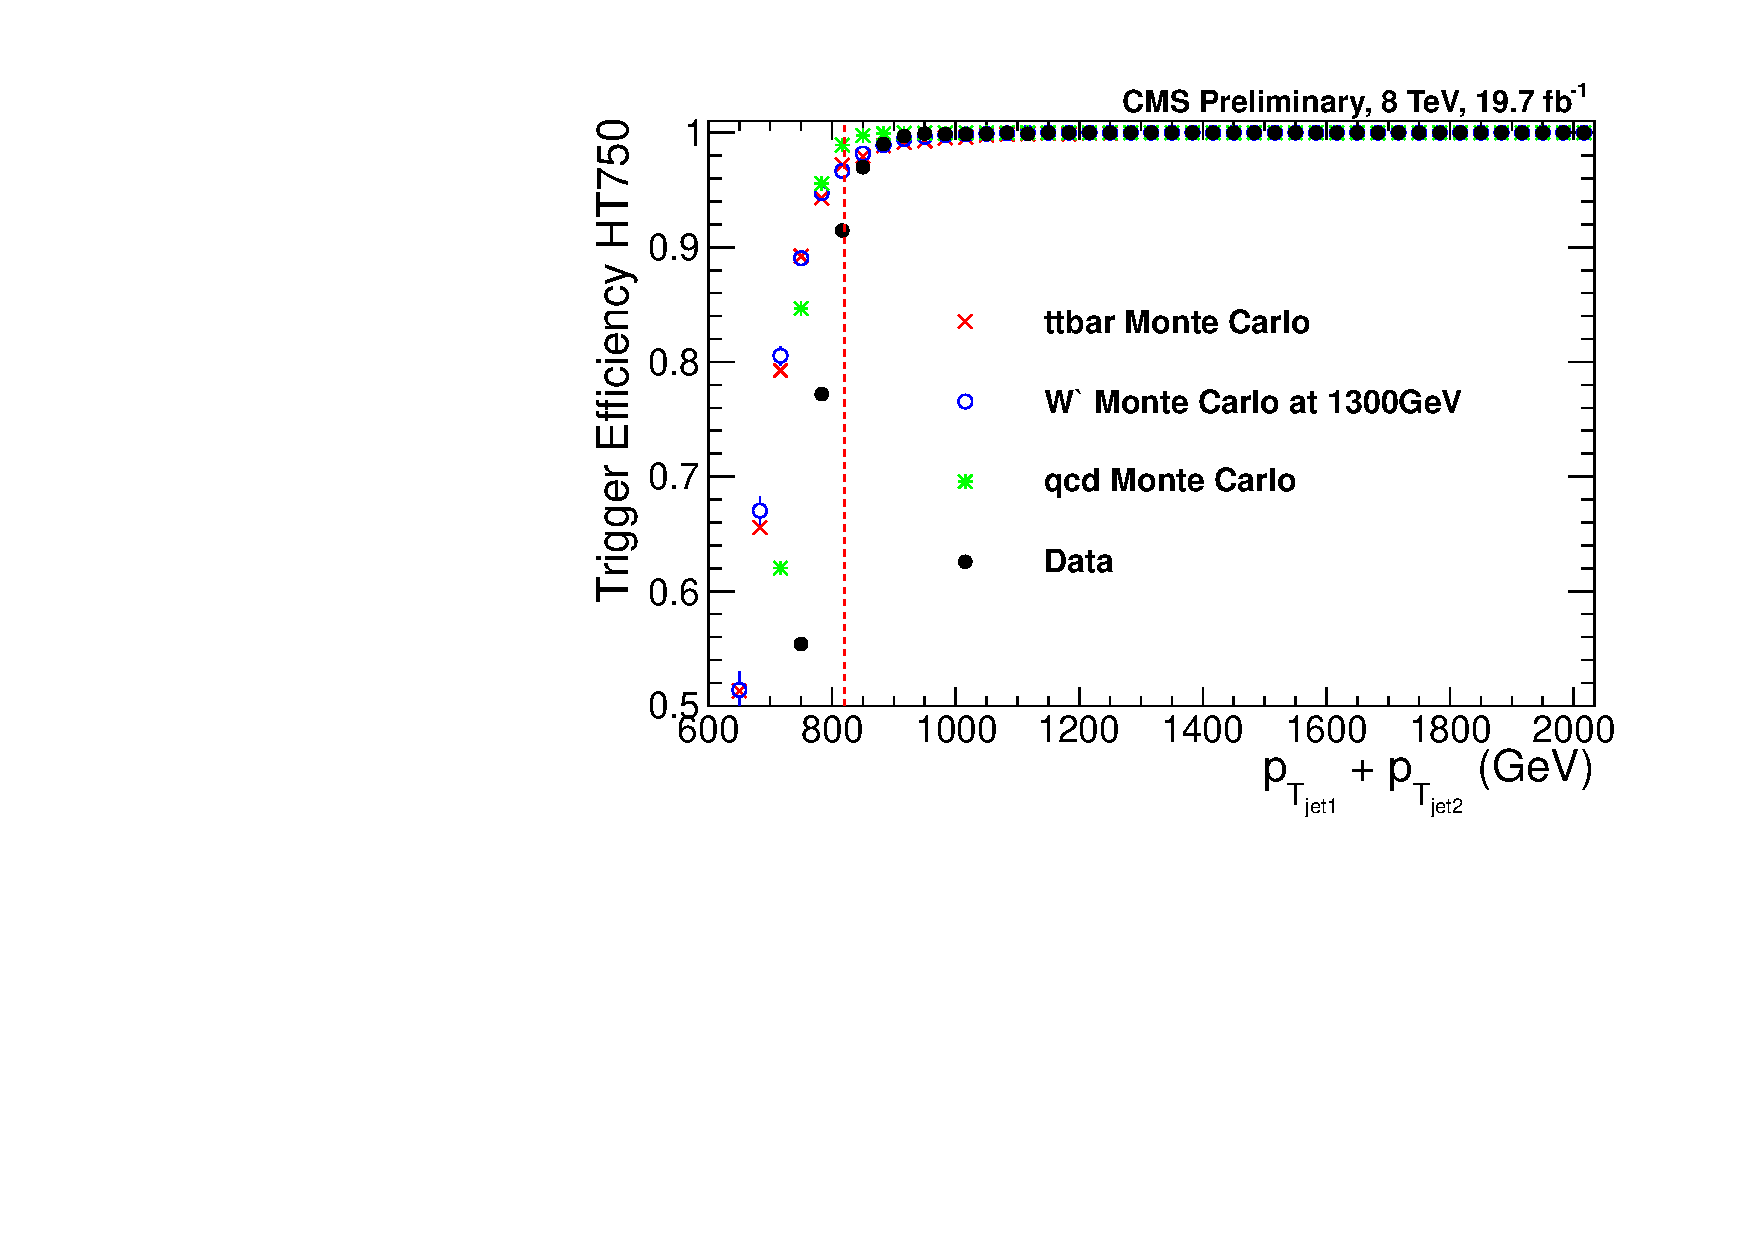
\includegraphics[width=0.9\textwidth]{AN-13-004/figs/Trigger_Comparison_Htdijet.pdf}
\caption{Trigger efficiency of \texttt{HLT\_HT750} measured as a function of the summed $\pt$ of the leading and sub-leading jets.  The red dashed line indicates the minimum for the analysis, 
at which point the trigger is nearly fully efficient.}
\label{figs:Trigger_Comparison_Ht}
\end{figure}

\section{Signal Characteristics}
\label{sec:sigchar}
\label{sec:GenBptCut}
The $\wpr$ boson of interest is very massive, and produces highly boosted top quarks.  The decay products of these top quarks become more collimated as the boost 
increases.  When the top decays hadronically, we observe one merged jet over the two distinct jets that would be detected at a lower boost.  This jet has a 
large characteristic radius and a distinct substructure.  This high energy jet merging is investigated in Figure \ref{figs:topmerge}.  Here, the `top candidate' 
is just the leading jet in the event.  It is also required to be hemispherically separated from a Monte Carlo truth b jet.  This jet is generally a merged W boson at low $\pt$ and a merged top at high $\pt$.
The `W candidate' (used for the bottom plots) is assembled from the pair of generator level non-b quarks that are close to the W mass (within 2.0~$\GeV$).  
The central feature of this analysis is using this jet merging to discriminate signal from background.

\begin{figure}[htcb]
\centering
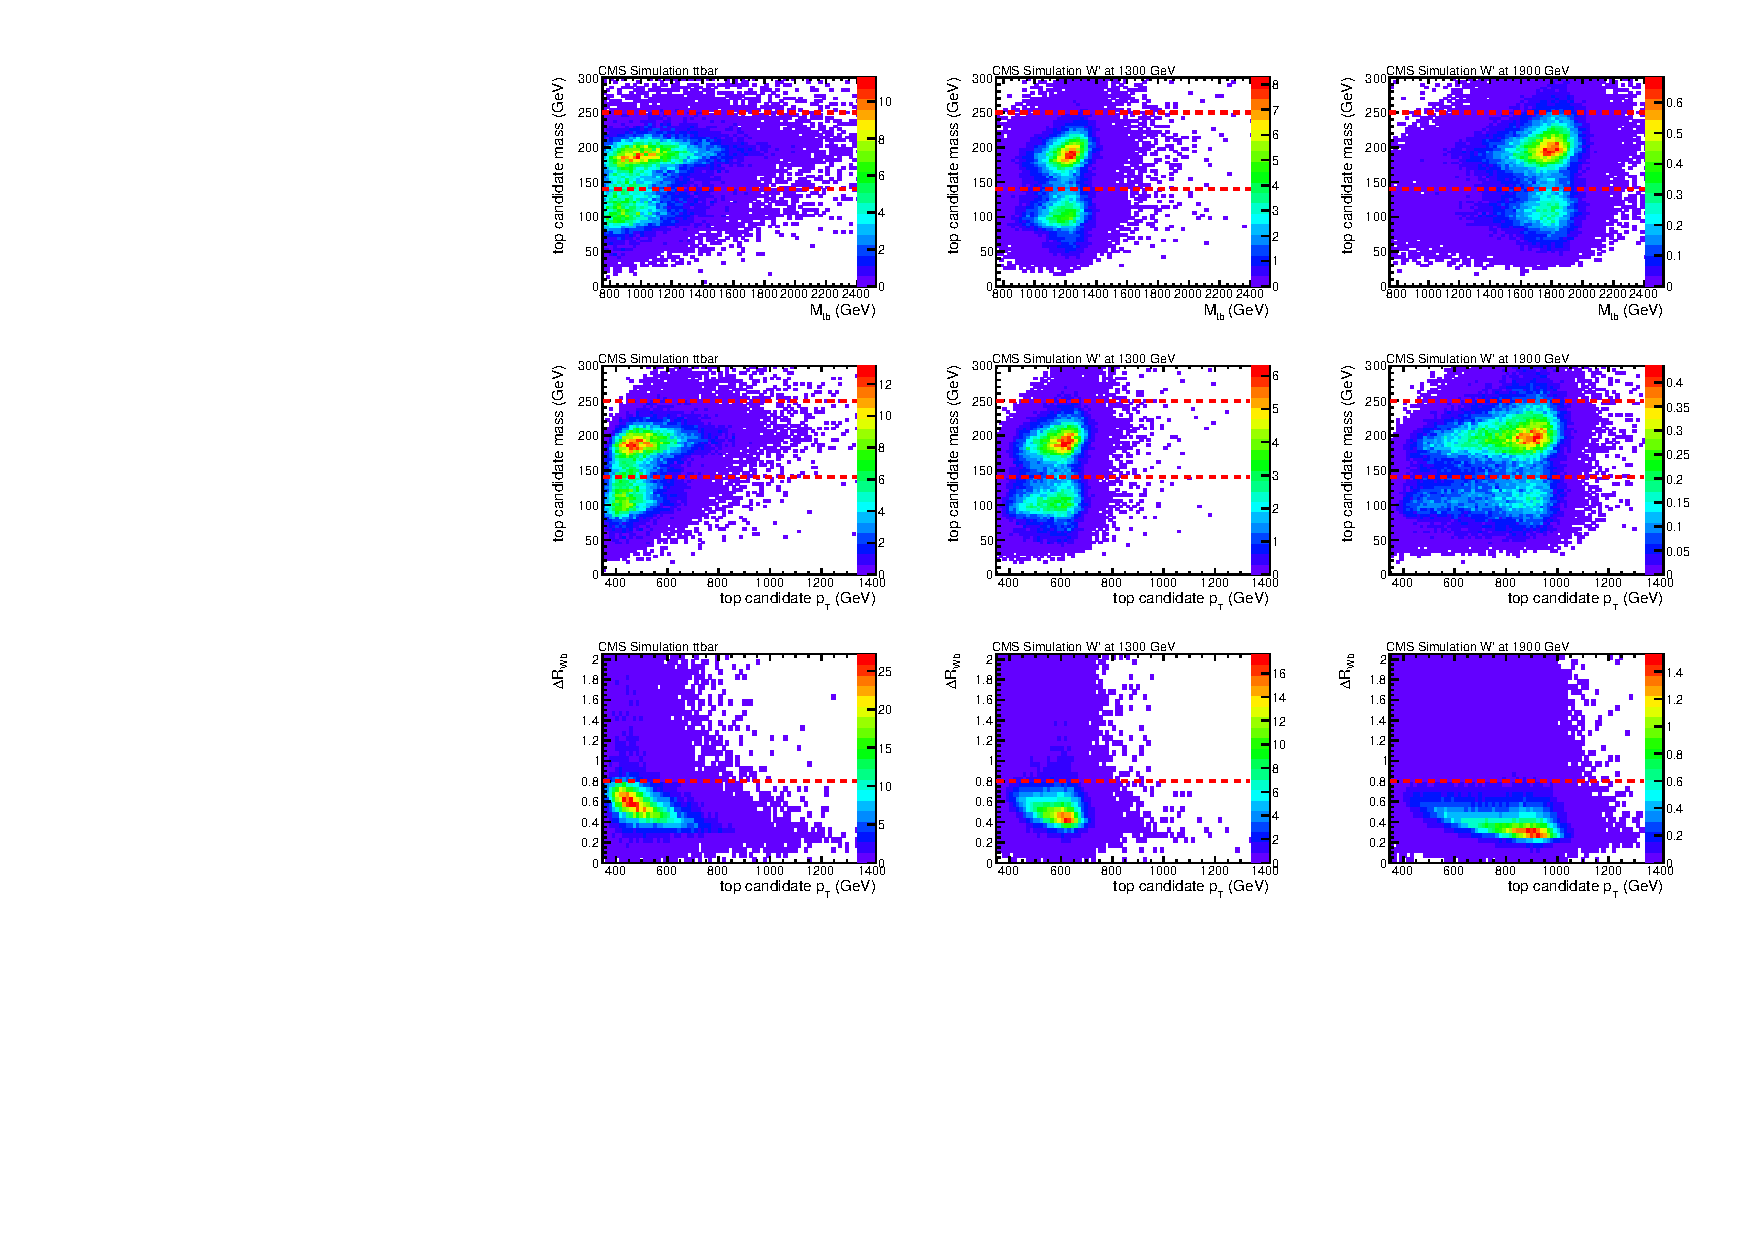
\includegraphics[width=0.9\textwidth]{AN-13-004/figs/topmerge.pdf}
\caption{Investigation of top merging within Monte Carlo samples of interest.  $\ttbar$ (left) $\wpr_R$ Monte Carlo at 1300$\GeV$ (middle) $\wpr_R$ Monte Carlo at 1900$\GeV$ (right).  The red lines on the top and middle plots indicate the top candidate mass cut in the full selection (see Section \ref{sec:toptagging}).  The red line on the bottom plots indicate the characteristic jet radius used to investigate fully merged top jets (see Section \ref{sec:reconstruction}).}
\label{figs:topmerge}
\end{figure}

We place a generator level $\pt$ cut on the b quark from the $\wpr$ decay in the left-handed and mixed-coupling $\wpr$ samples (see Section \ref{sec:signal}).  
To investigate the effect of this pre-selection, we look at the effect of an even tighter cut.  
Figure \ref{figs:genptcut} shows the ratio of generator level b $\pt$ cuts.  
The denominator requires a generation level pt cut of 200 $\GeV$ and the numerator requires a generation level pt cut of 230 $\GeV$.  
This ratio is parameterized in the $\pt$ of the CA8 jet that the generation particle is matched to ($\mathrm{\Delta R  < 0.5}$ is used for matching).
The turn on of this tighter cut is well below the analysis level cut of 370$~\GeV$.  Thus, the effect of the generation level b $\pt$ cut 
on selections requiring the analysis level $\pt$ cut is negligible.  

\begin{figure}[Htcb]
\centering
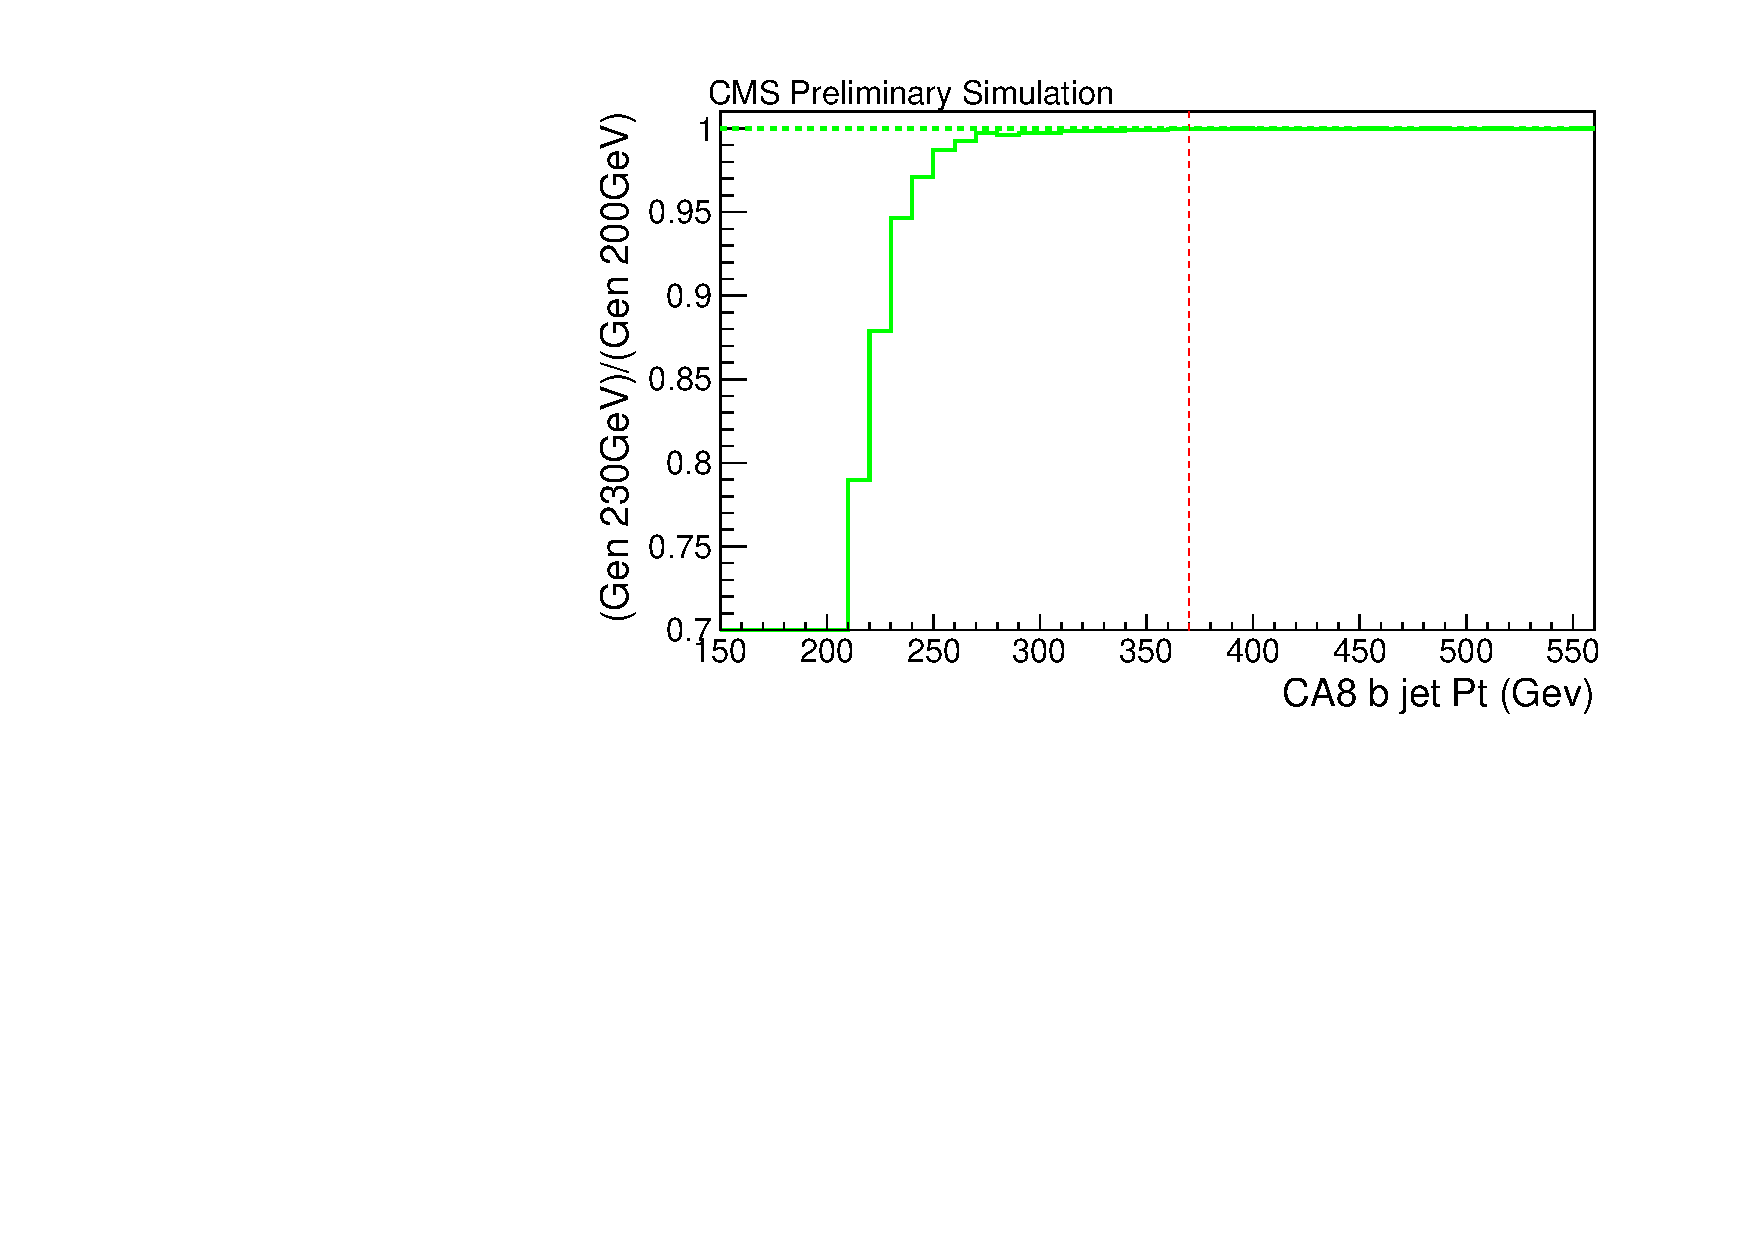
\includegraphics[width=1.0\textwidth]{AN-13-004/figs/bjetptcut.pdf}
\caption{Ratio of CA8 $\pt$ using the generation level b pt cut of 230$~\GeV$ and 200$~\GeV$.  The red line is the analysis level $\pt$ cut of 370$~\GeV$.  The sample used for this study is $W`_{LR}$ at 1300$~\GeV$}
\label{figs:genptcut}
\end{figure}



\section{Jet Reconstruction}
\label{sec:reconstruction}
All data is reconstructed using CMSSW 5.3.x, and uses jet energy corrections from \verb!FT_53_V21_AN5! \cite{CMS-DP-2013-033}.  The Particle Flow reconstruction algorithm is used 
to reconstruct all data and Monte Carlo samples used for the analysis.  This algorithm uses information from all sub-detectors 
to categorize particles as muons, electrons, photons as well as charged and 
neutral hadrons.  Charged hadrons identified as pileup are removed from the inputs to the jet clustering algorithms by Charged Hadron Subtraction (CHS).
Pileup vertices are identified as vertices that have a lower $\pt$ than the primary vertex.  Isolated charged leptons are removed,
and neutral pileup components are removed with a residual area-based method.  For more detail, see \cite{7tevZprime}.  
The PF candidates are then used to create 'Particle Flow jets' as follows.  Jet clustering is performed 
with a sequential recombination algorithm which compiles jets by merging the minimum of 
$\mathrm{d_{ij} = min(k_{Ti}^{2m},k_{Tj}^{2m})\Delta _{ij}/R}$ where $\mathrm{\Delta _{ij} = \sqrt{(y_i-y_j)^2 + (\phi _i-\phi _j)^2}}$.
  We use the Cambridge-Aachen (CA) \cite{CAcambridge,CAaachen} algorithm implemented by FastJet 3 \cite{fastjet1,fastjet2}, 
which assigns a value of $\mathrm{m = 0}$, and thus is not weighted by $\pt$.  An R value 
of 0.8 is used for the analysis.  The CA algorithm has been shown to be more efficient than the 
the $\mathrm{k_{T}}$ and the anti-$\mathrm{k_{T}}$ algorithms for finding hard subjets \cite{catop_cms}.

%The corrections for the CA $R=0.8$ jets are derived from the
%anti-$k_{\mathrm T}$ $R=0.7$ jet algorithm. 
We use anti-$\mathrm{k_{T}}$ jet energy corrections for all jets in the analysis. 
The jet energy corrections derived are adequate for the CA $\mathrm{R=0.8}$ jet algorithm for the jet momenta
considered here as can be seen from 7~$\TeV$ studies in simulation comparing AK5 and CA8 jets \cite{7tevZprime}.  
We use the 2012 prescription for jet energy corrections\cite{JEC2012}.  We apply AK7 
Particle Flow with charged hadron subtraction 
(AK7PFchs) jet energy corrections for all data and Monte Carlo samples.

\section{Event Pre-selection}
\label{sec:pre-selection}
The following pre-selection is applied:

\begin{itemize}
\item The event must have a good primary vertex as computed by a deterministic annealing filter (DAF)
($\vert z_\text{Primary Vertex}\vert < 24$ cm, $N_\text{DOF} > 6$).
\item Two jets with $|y| < 2.4$
\item Only two jets with $\pt > 150~\GeV$
\item Leading Jet $\pt > 450~\GeV$ \& Sub-leading Jet $\pt > 370~\GeV$
\item Loose Particle Flow jet identification \cite{jetid} is applied
\item Leading and sub-leading jet are separated by $|\Delta y| < 1.6$
	\begin{itemize}
	\item This cut is described in Section \ref{sec:deltarapidity}
	\end{itemize}
\item Beam background events are removed using the following requirements:
        \begin{itemize}
        \item In events with at least 10 tracks, a minimum of 25\% of
          these tracks must be high purity tracks.
        \end{itemize}
\end{itemize}


The requirement that there are only two jets with $\pt > 150~\GeV$ is useful for vetoing "three-prong" trijet events, which could impact the kinematics of the top-W candidate invariant mass 
distribution and bias the background estimate. 

\section{$\ttbar$ $\pt$ Re-weighting}
\label{sec:ttptrw}
In order to correct for known differences in the top $\pt$ spectrum between data and $\ttbar$ Monte Carlo, we re-weight Monte Carlo using the Generator level $\pt$ of the top and anti-top with the recommended prescription.  
With $\mathrm{p_{T_{t}}}$ and $\mathrm{p_{T_{\overline{t}}}}$ being the generator $\pt$ of the top and anti-top respectively, the scale factor applied to each event in the $\ttbar$ Monte Carlo expectation is:
\begin{eqnarray}
SF =\sqrt{e^{0.156-.00137p_{T_{t}}} \times e^{0.156-.00137p_{T_{\overline{t}}}}}
\end{eqnarray}
Although this procedure was not designed for the kinematic range in our analysis, we prefer to use the prescription as it is more consistent with our measurement of the $\ttbar$ normalization (see Section \ref{sec:ttbarsideband}).


\section{Pileup Correction}
\label{sec:pileup}
We re-weight our Monte Carlo samples to account for differences due to pileup using the recommended procedure.  
To create a scale factor for number of primary vertices, we use Monte Carlo truth to extract the number of pileup interactions.  
Then we compare this to the mean number of interactions per crossing from data.  
This is extracted using the pileup distribution from the rereco datasets listed in table \ref{table:datasets}.  
For this calculation we use the suggested minbias cross-section of 69.4 mb.  The scale factor is then 
the data distribution divided by the distribution in Monte Carlo and is applied to the signal and $\ttbar$ Monte Carlo samples to improve 
data to Monte Carlo agreement.
Figure \ref{figs:npvweight} shows the distribution of reconstructed primary vertices in Data, $\ttbar$,
and signal Monte Carlo before and after the re-weighting has been applied. The pileup correction has very little effect on the eventual $\mathrm{M_{tb}}$ full selection, as 
seen in Figure \ref{figs:pileup3}, for $\wpr_R$ signal Monte Carlo at the 1900$~\GeV$ mass point. Similarly, there is little effect 
$\ttbar$ Monte Carlo as can be seen in Figure \ref{figs:pileup3ttbar}.  
A study has been conducted to investigate the effect of the suggested systematic uncertainty of 5\% on the  as can be seen in Chapter \ref{sec:systematics}.  
Figure \ref{figs:PUplots} shows the number of primary vertices in data and signal Monte Carlo with respect to discrimination variables used to separate signal from background.

\begin{figure}[Htcb]
\begin{center}
\subfigure{\label{figs:sub_data}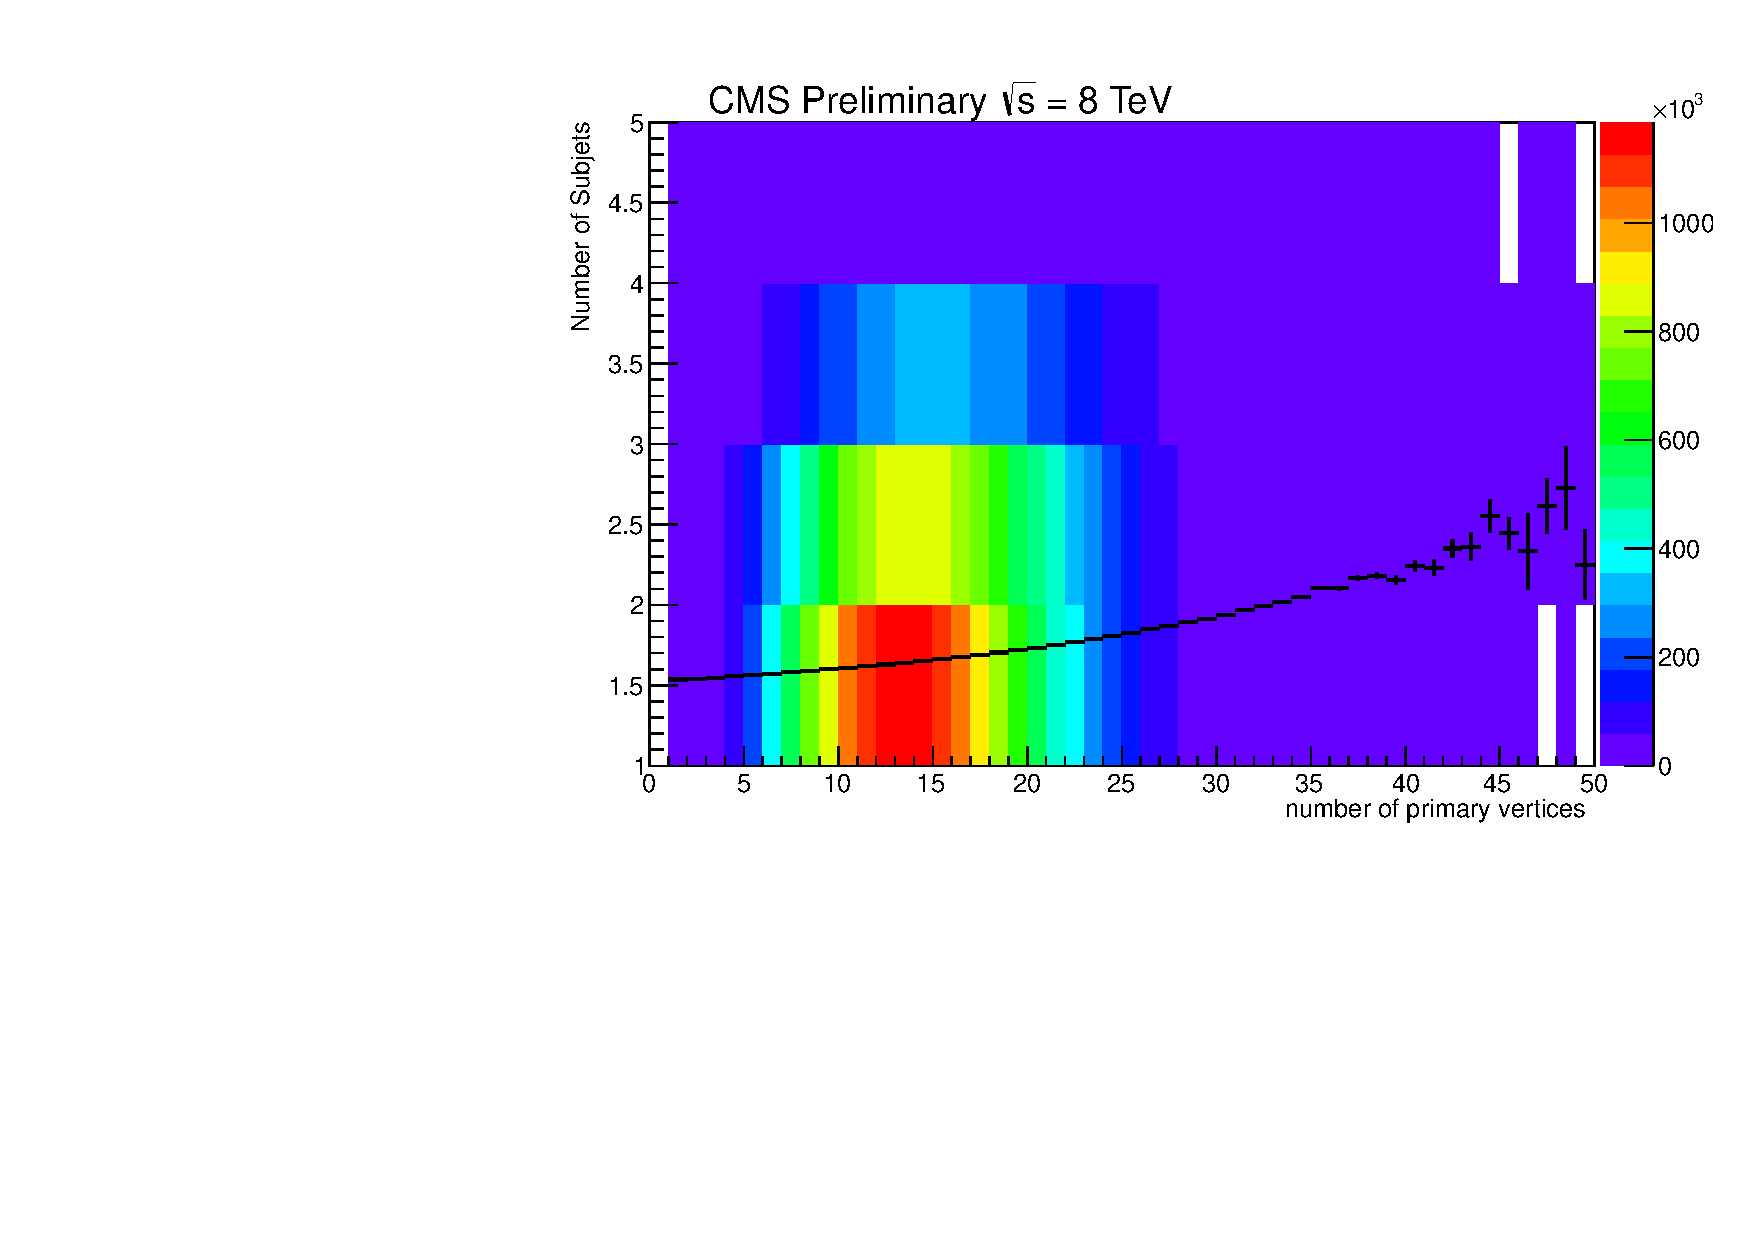
\includegraphics[width=0.4\textwidth]{AN-13-004/figs/sub_data.pdf}}
\subfigure{\label{figs:sub_signal}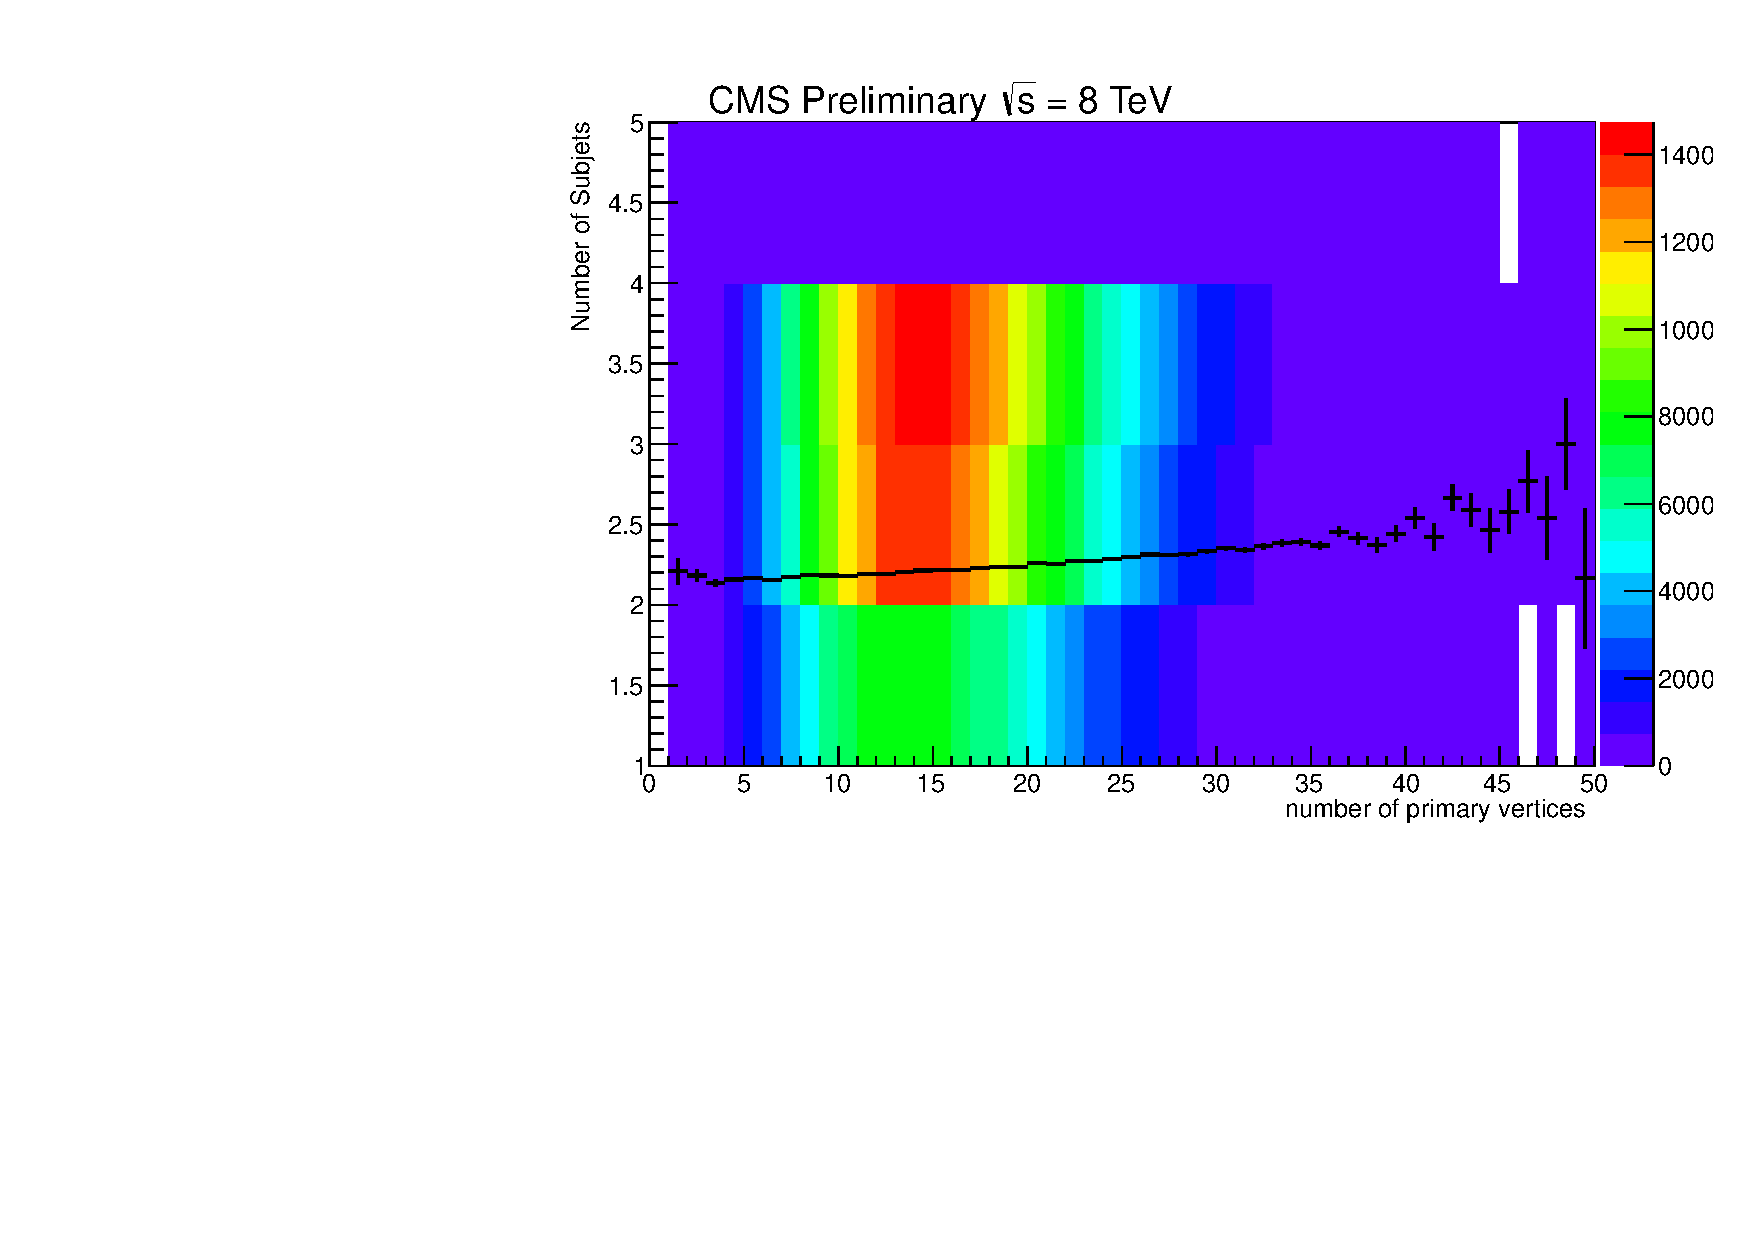
\includegraphics[width=0.4\textwidth]{AN-13-004/figs/sub_signal.pdf}}\\
\subfigure{\label{figs:min_data}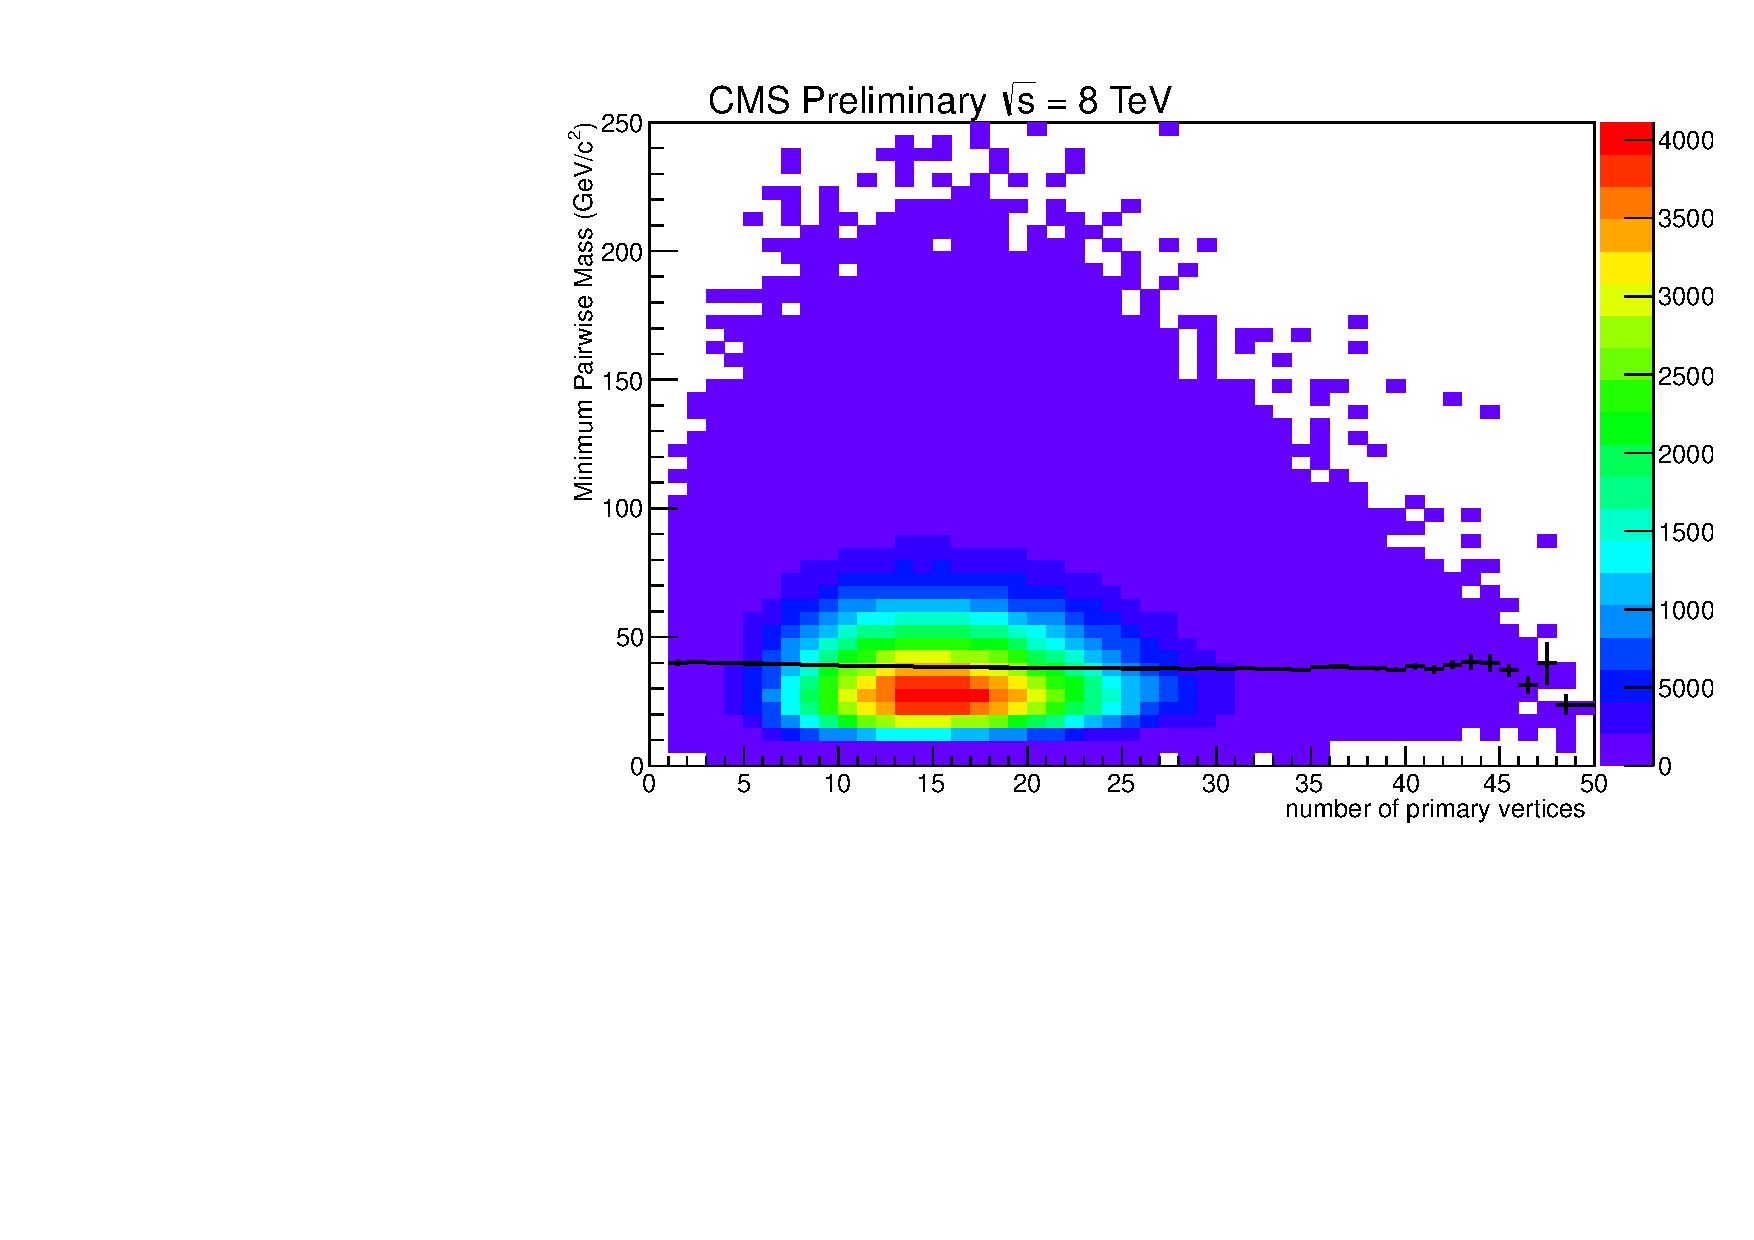
\includegraphics[width=0.4\textwidth]{AN-13-004/figs/min_data.pdf}}
\subfigure{\label{figs:min_signal}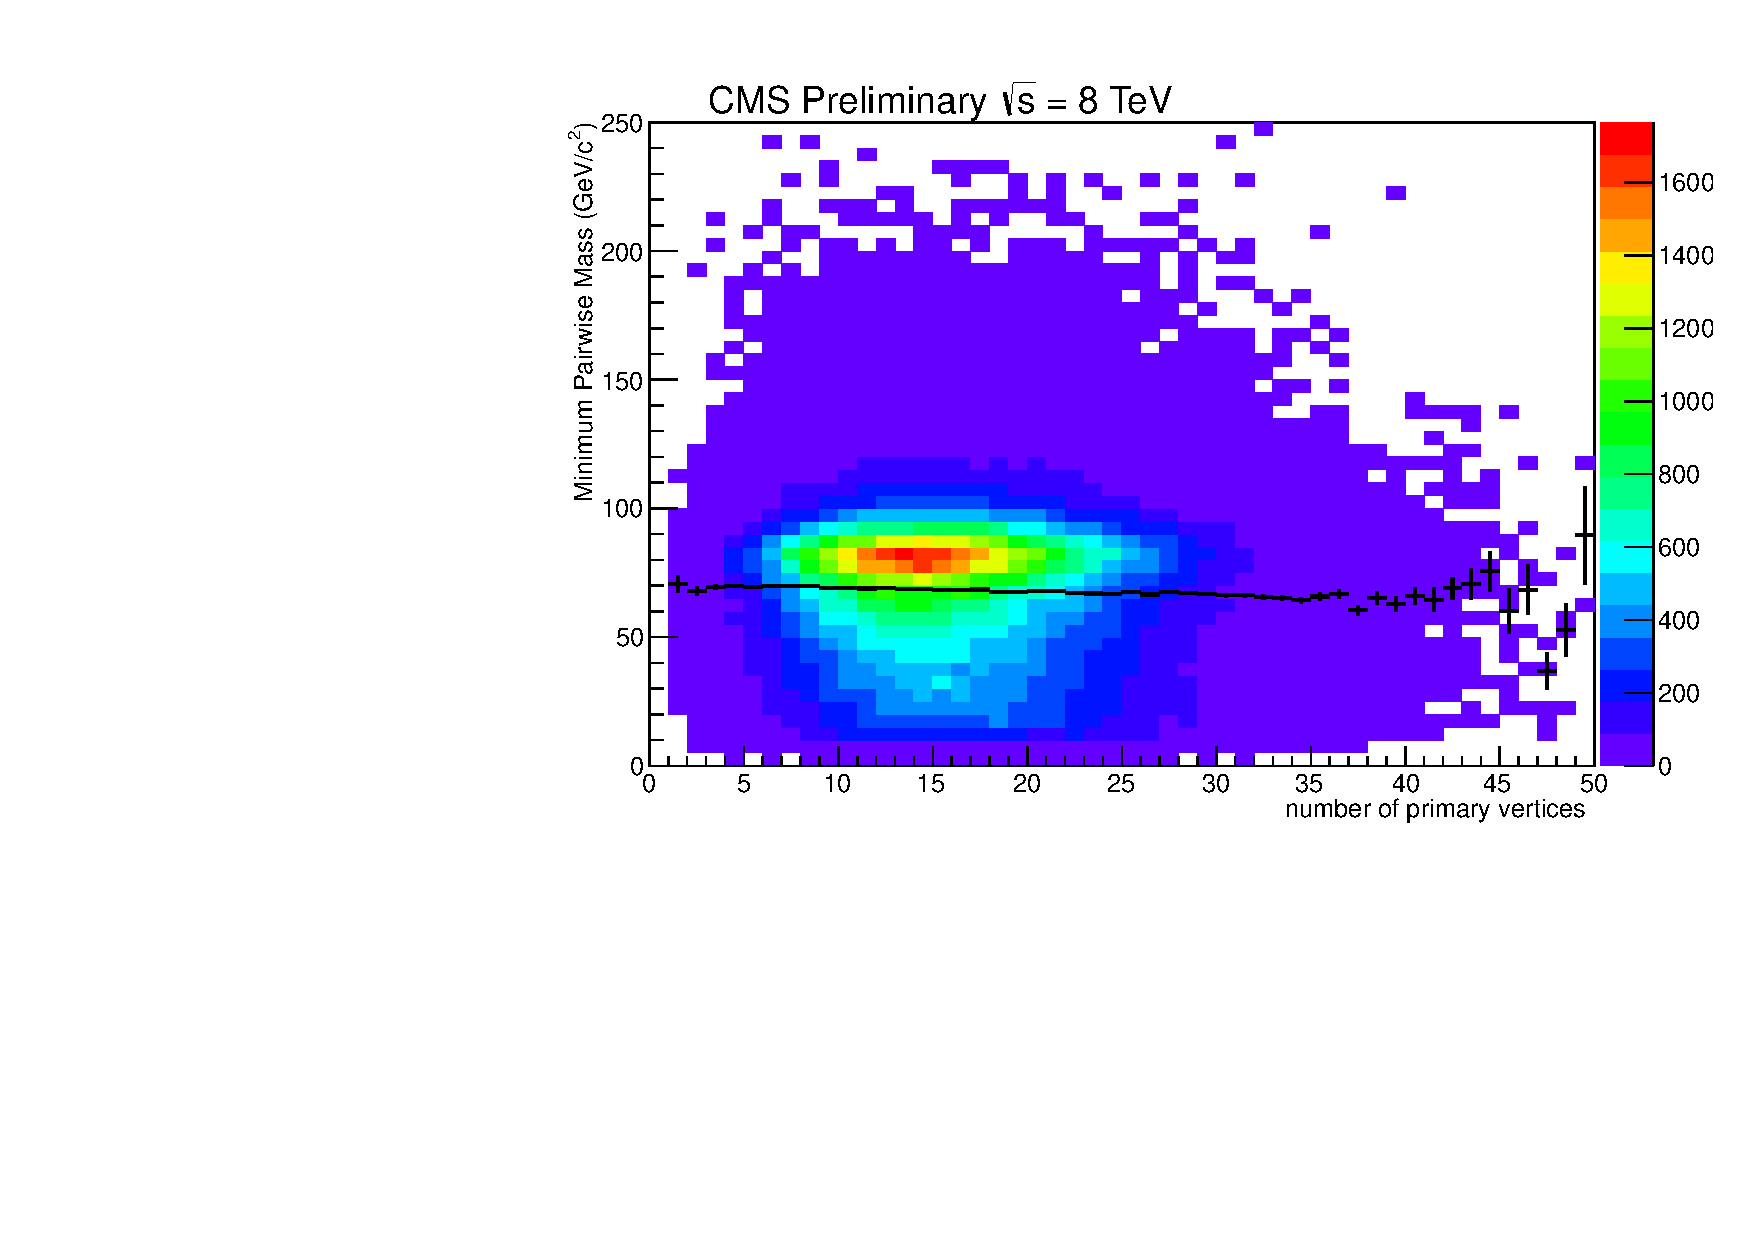
\includegraphics[width=0.4\textwidth]{AN-13-004/figs/min_signal.pdf}}\\
\subfigure{\label{figs:top_data}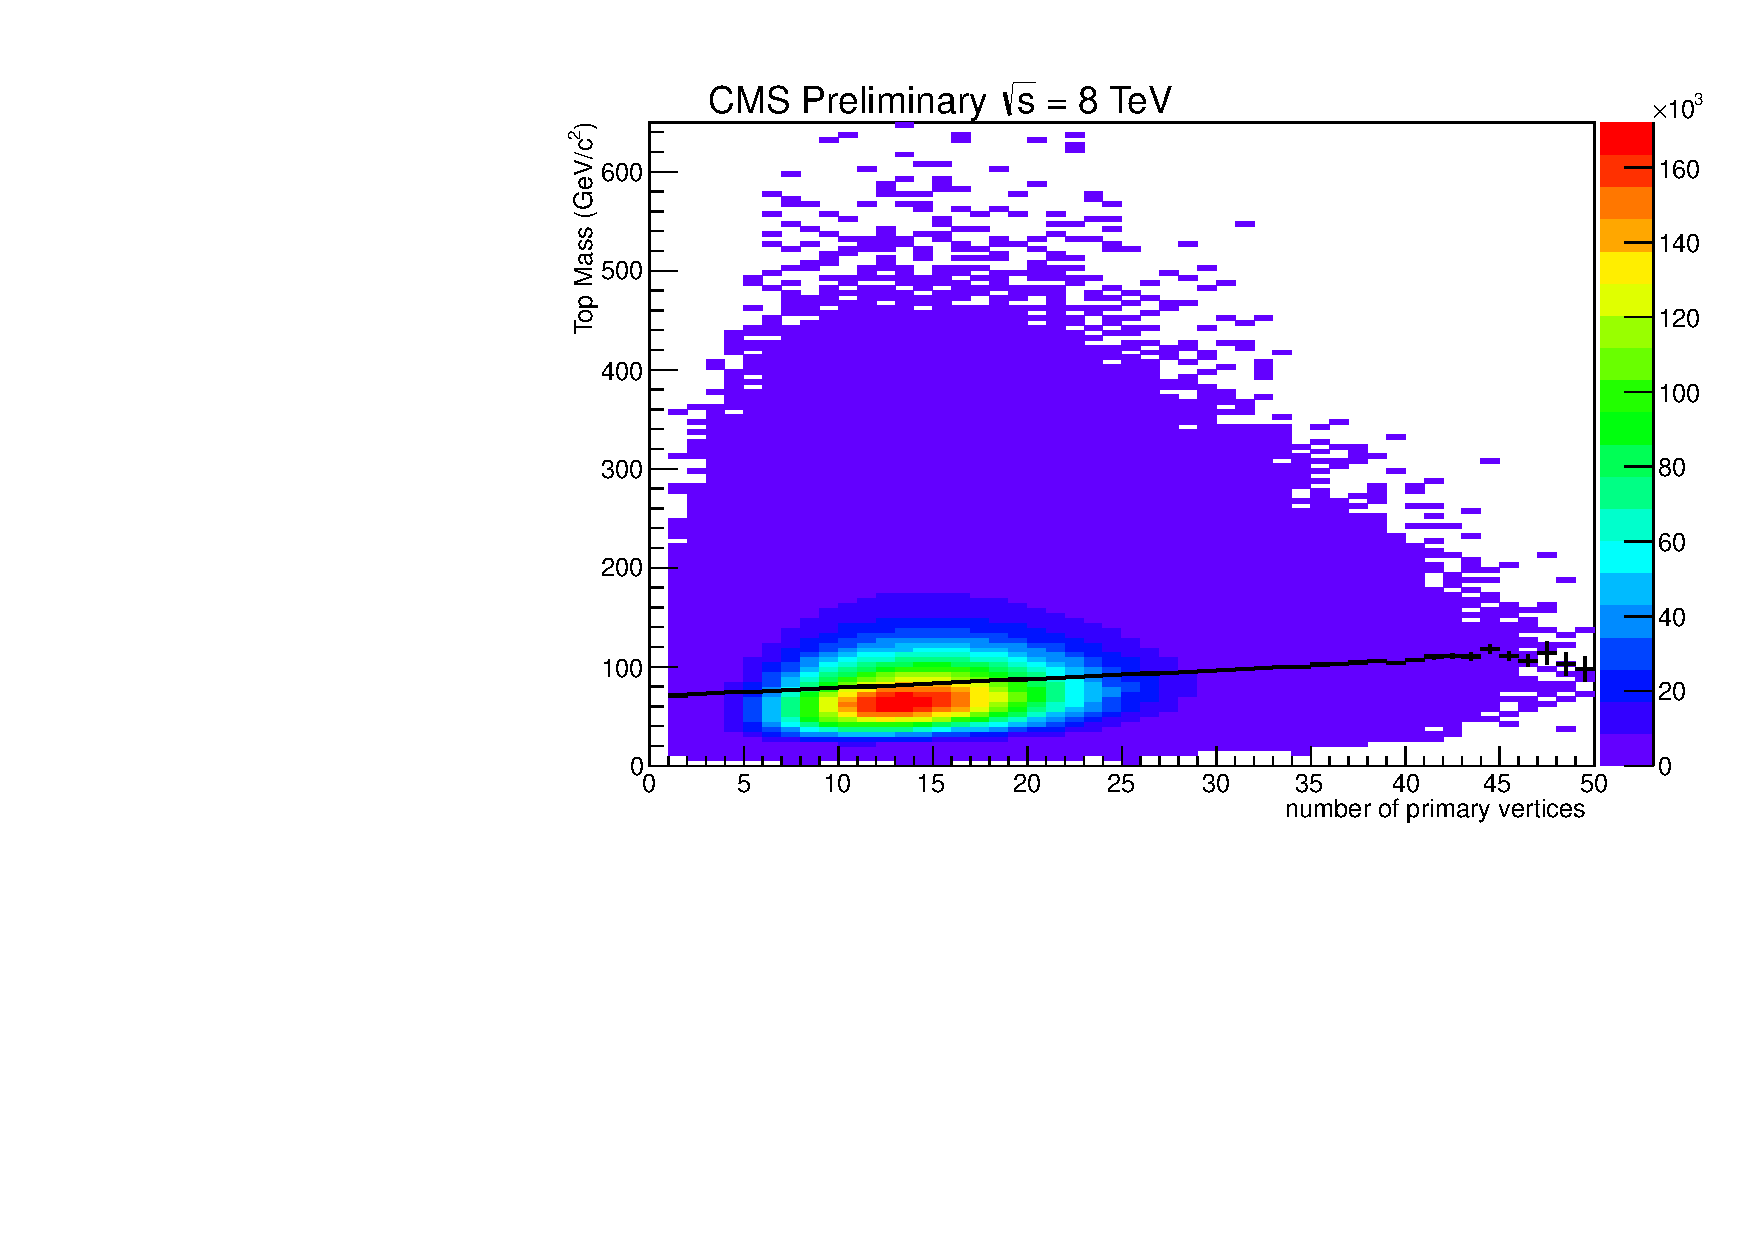
\includegraphics[width=0.4\textwidth]{AN-13-004/figs/top_data.pdf}}
\subfigure{\label{figs:top_signal}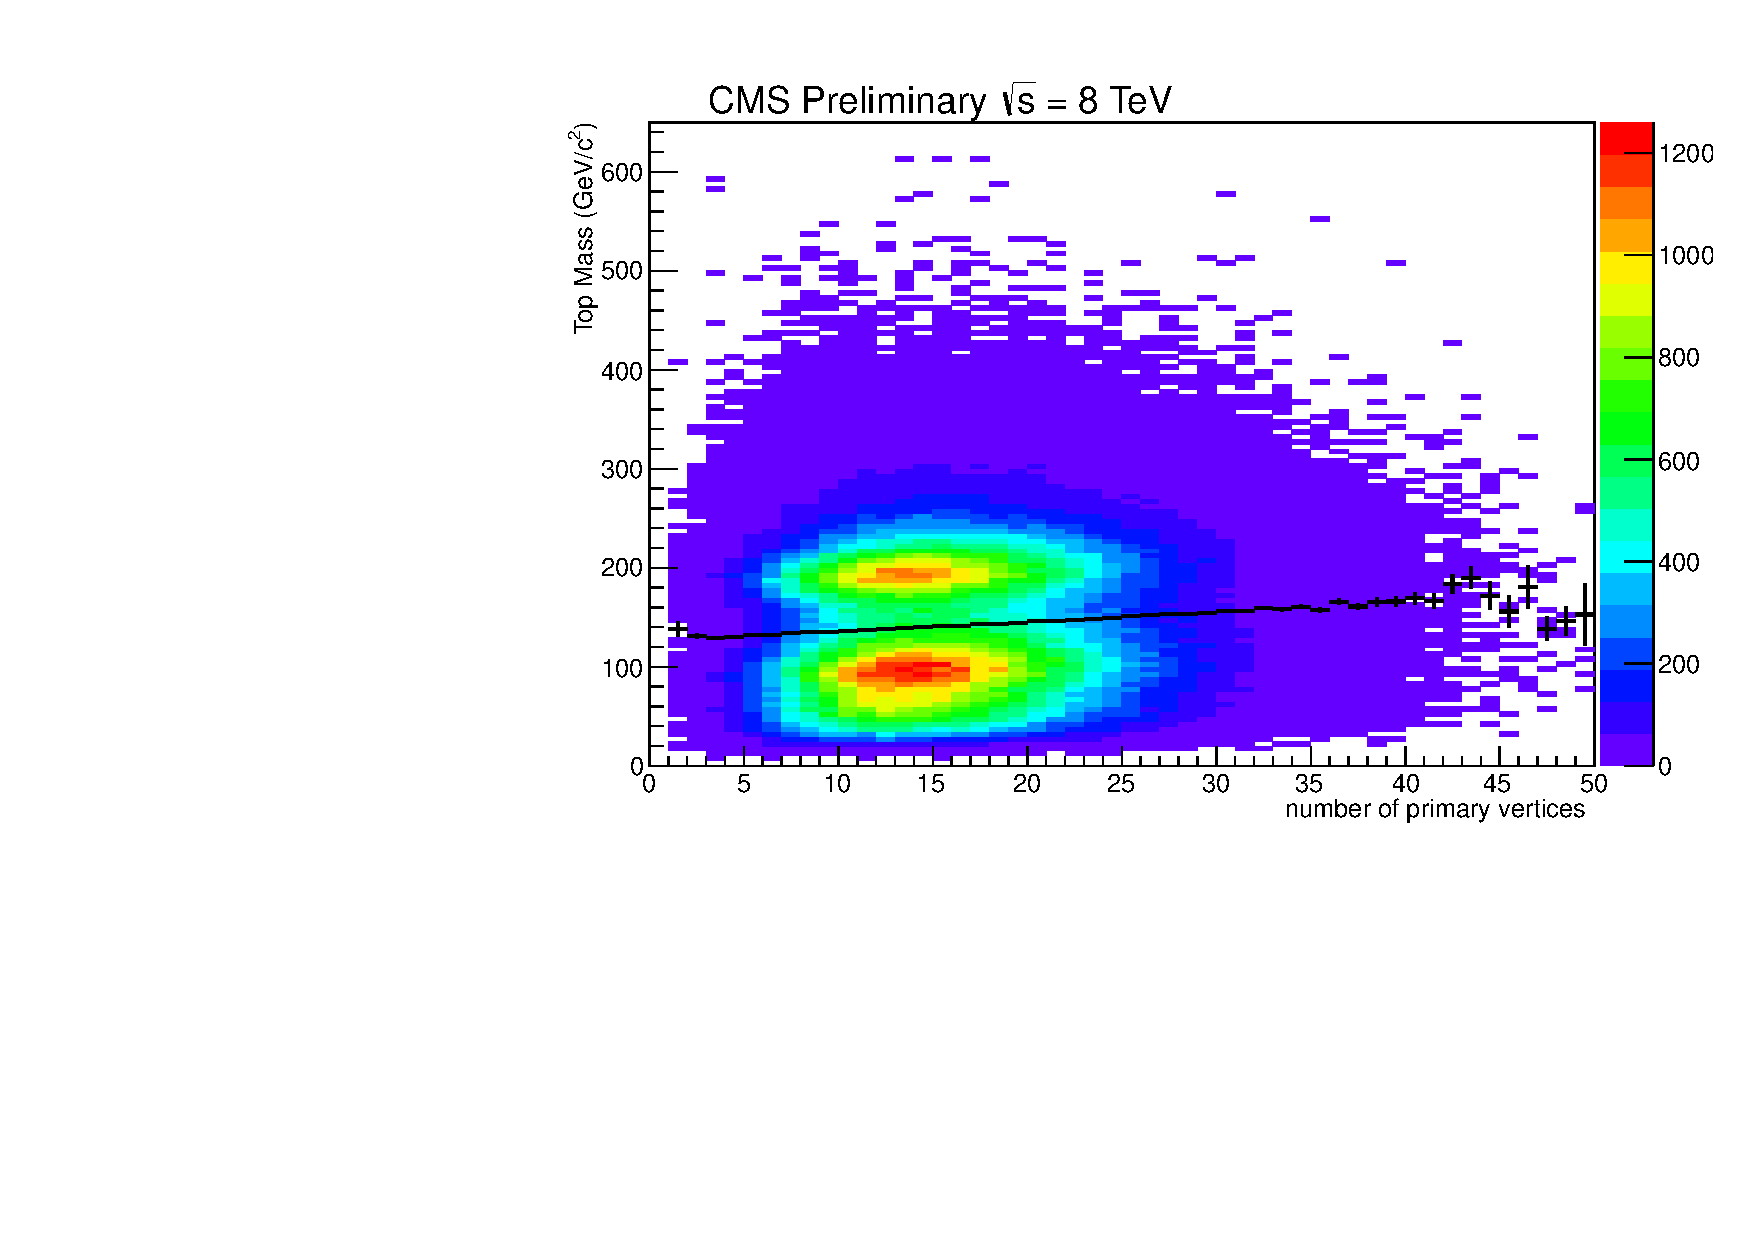
\includegraphics[width=0.4\textwidth]{AN-13-004/figs/top_signal.pdf}}\\
\subfigure{\label{figs:tag_data}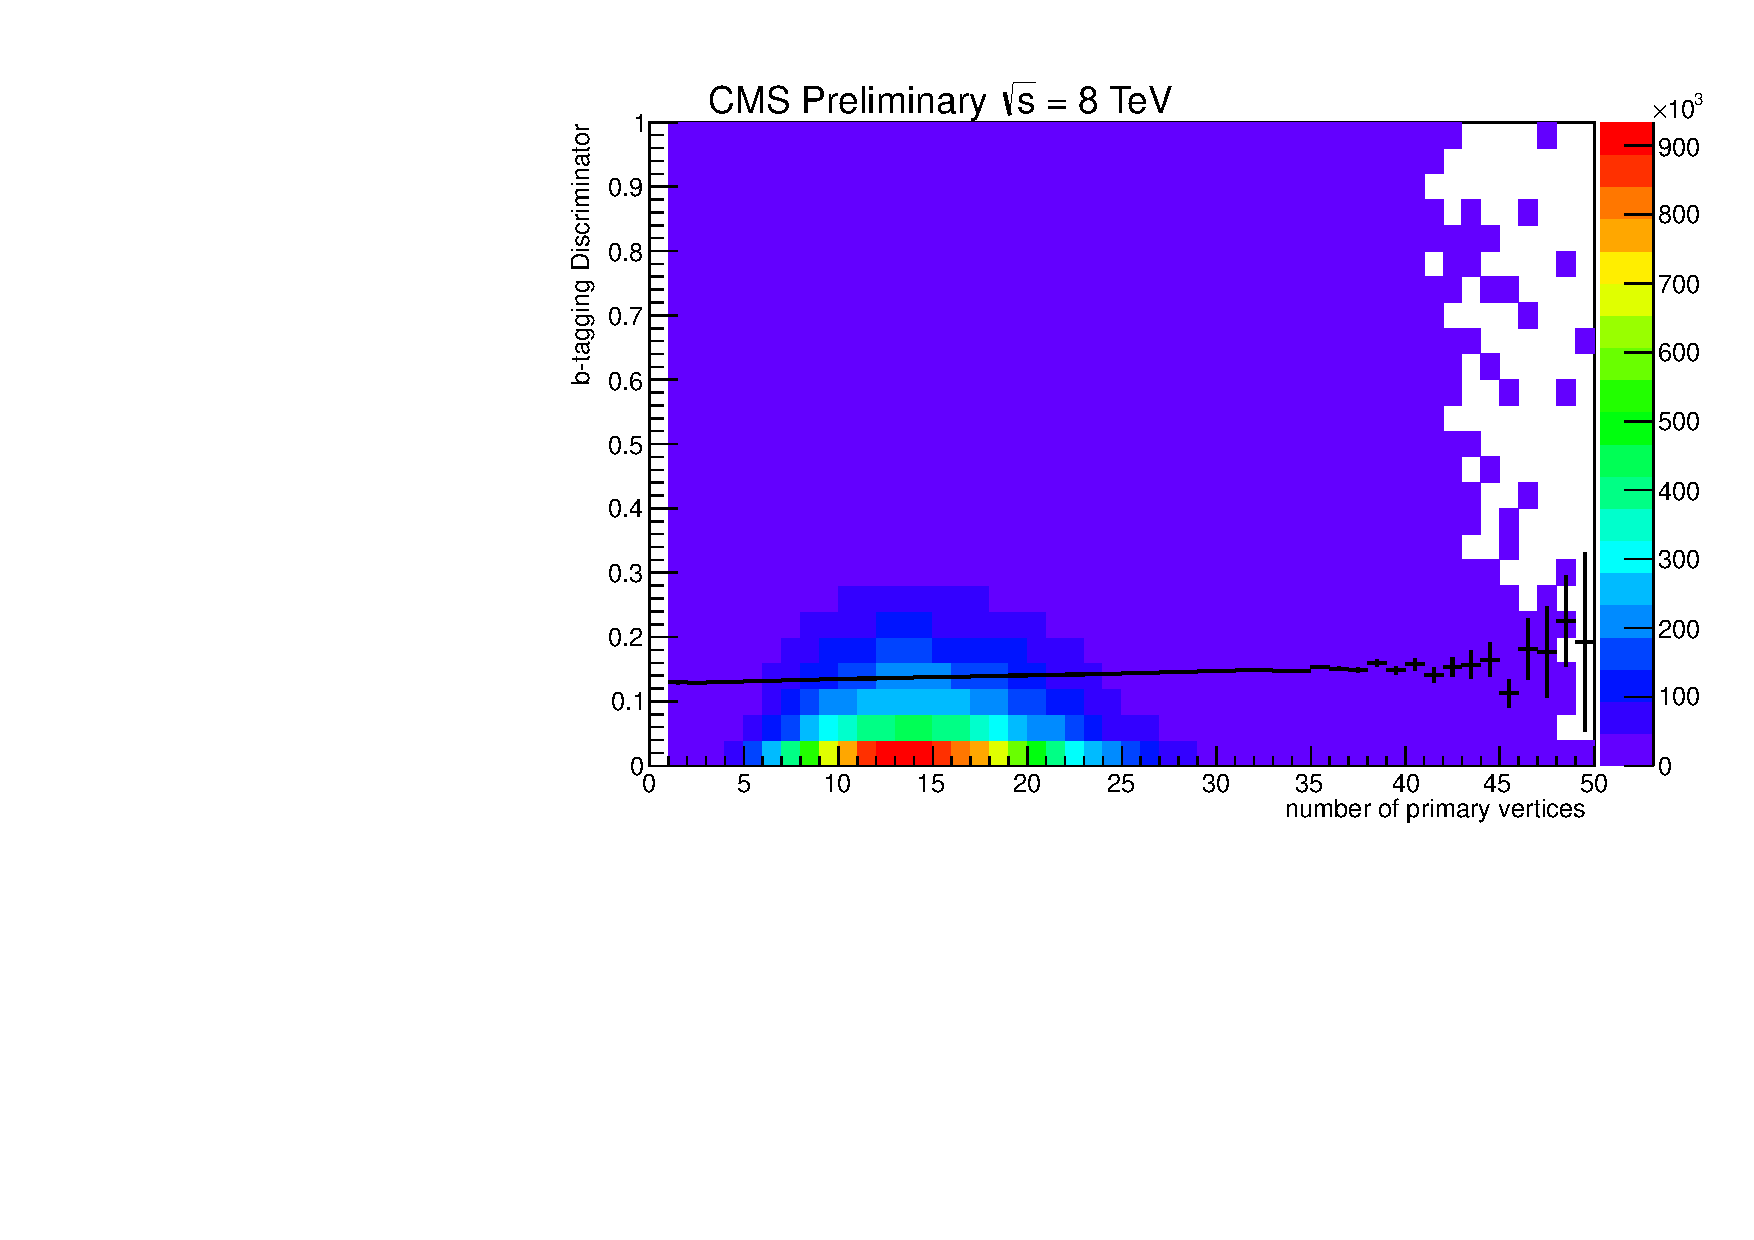
\includegraphics[width=0.4\textwidth]{AN-13-004/figs/tag_data.pdf}}
\subfigure{\label{figs:tag_signal}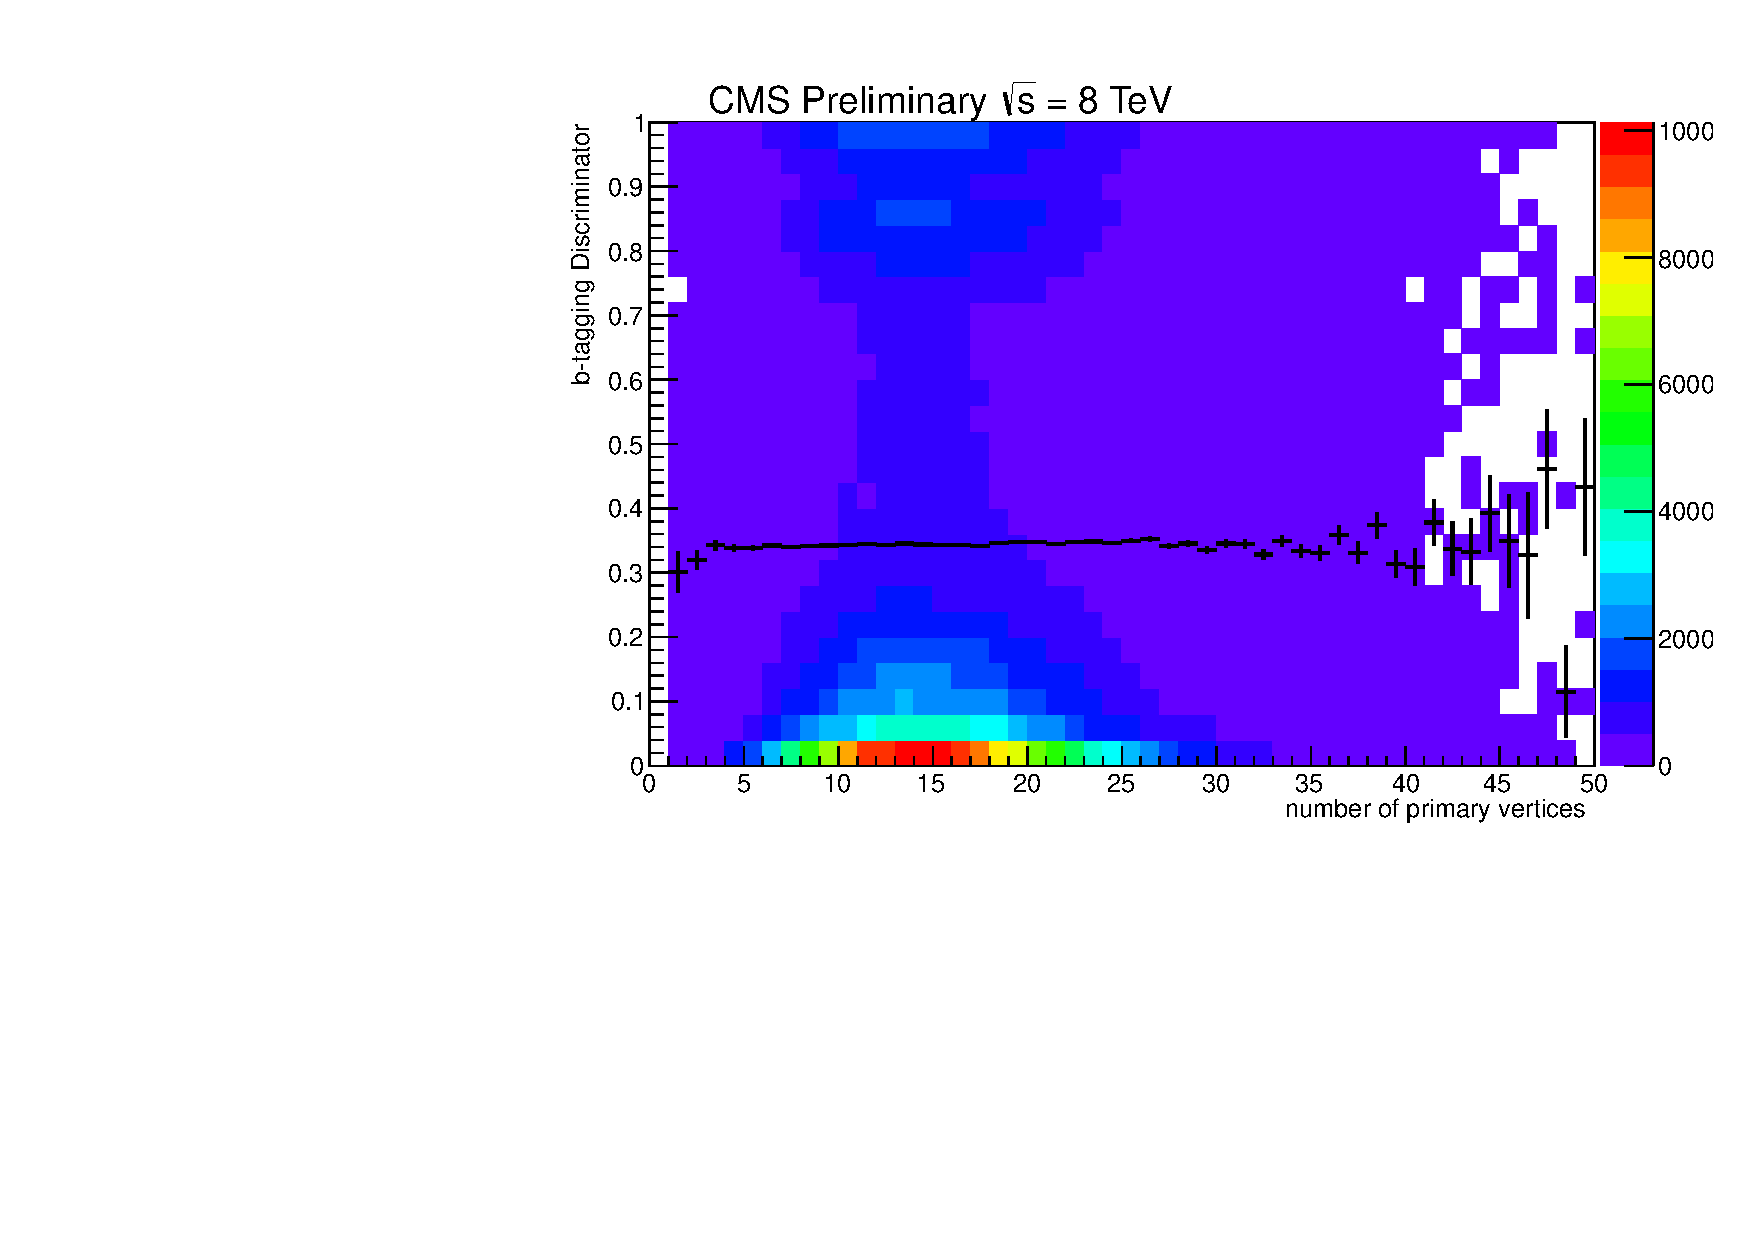
\includegraphics[width=0.4\textwidth]{AN-13-004/figs/tag_signal.pdf}}
\caption{
Number of primary vertices in data and signal Monte Carlo vs
(a) Number of Subjets  
(b) Minimum Pairwise Mass
(c) Top Mass
(c) CSV b discriminant 
}
\label{figs:PUplots}
\end{center}
\end{figure}


\begin{figure}
\begin{center}
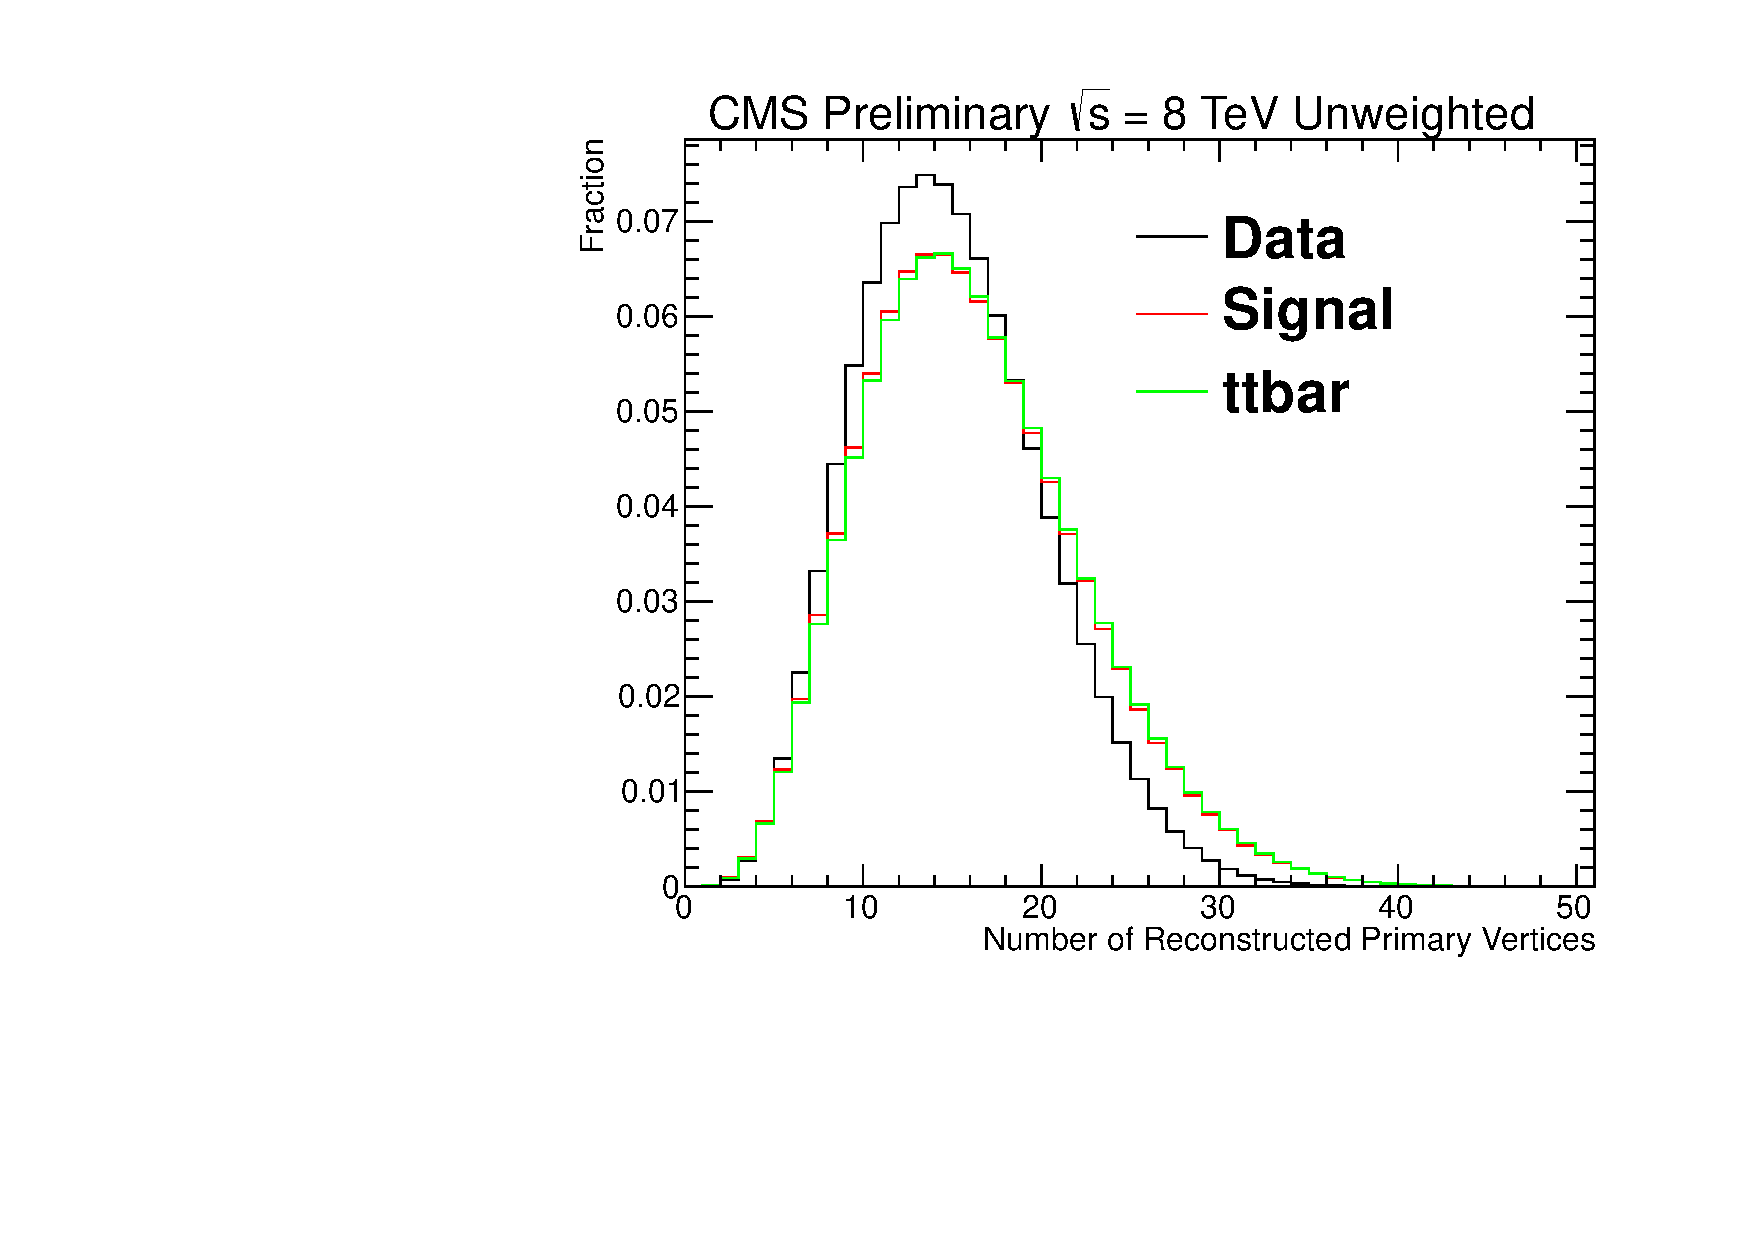
\includegraphics[width=0.7\linewidth]{AN-13-004/figs/npvuw.pdf}\\
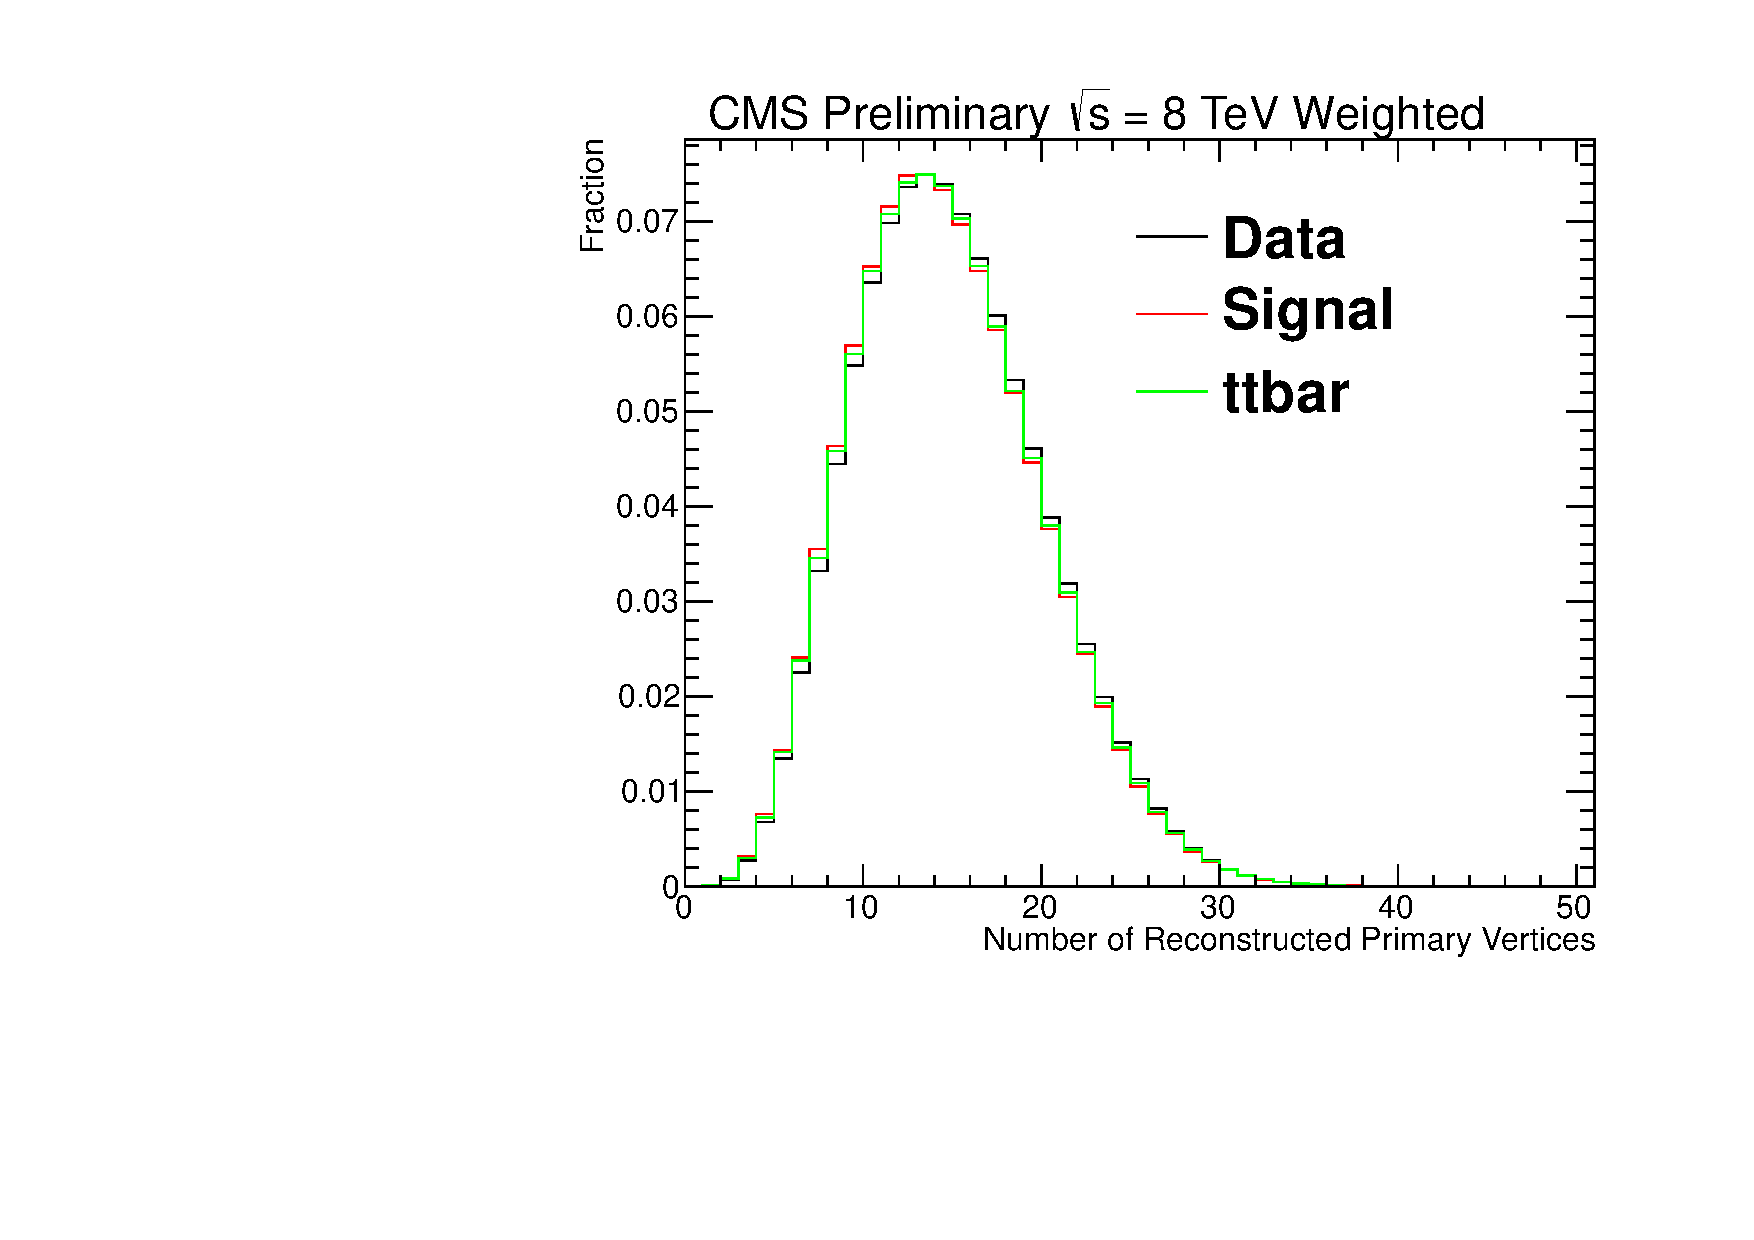
\includegraphics[width=0.7\linewidth]{AN-13-004/figs/npvw.pdf}
\end{center}
\caption{Number of reconstructed primary vertices before pileup re-weighting (top) and after pileup re-weighting (bottom).  Here, no analysis cuts have been applied and the signal mass point is 1900$~\GeV$}
\label{figs:npvweight}
\end{figure}

\begin{figure}[htcb]
\centering
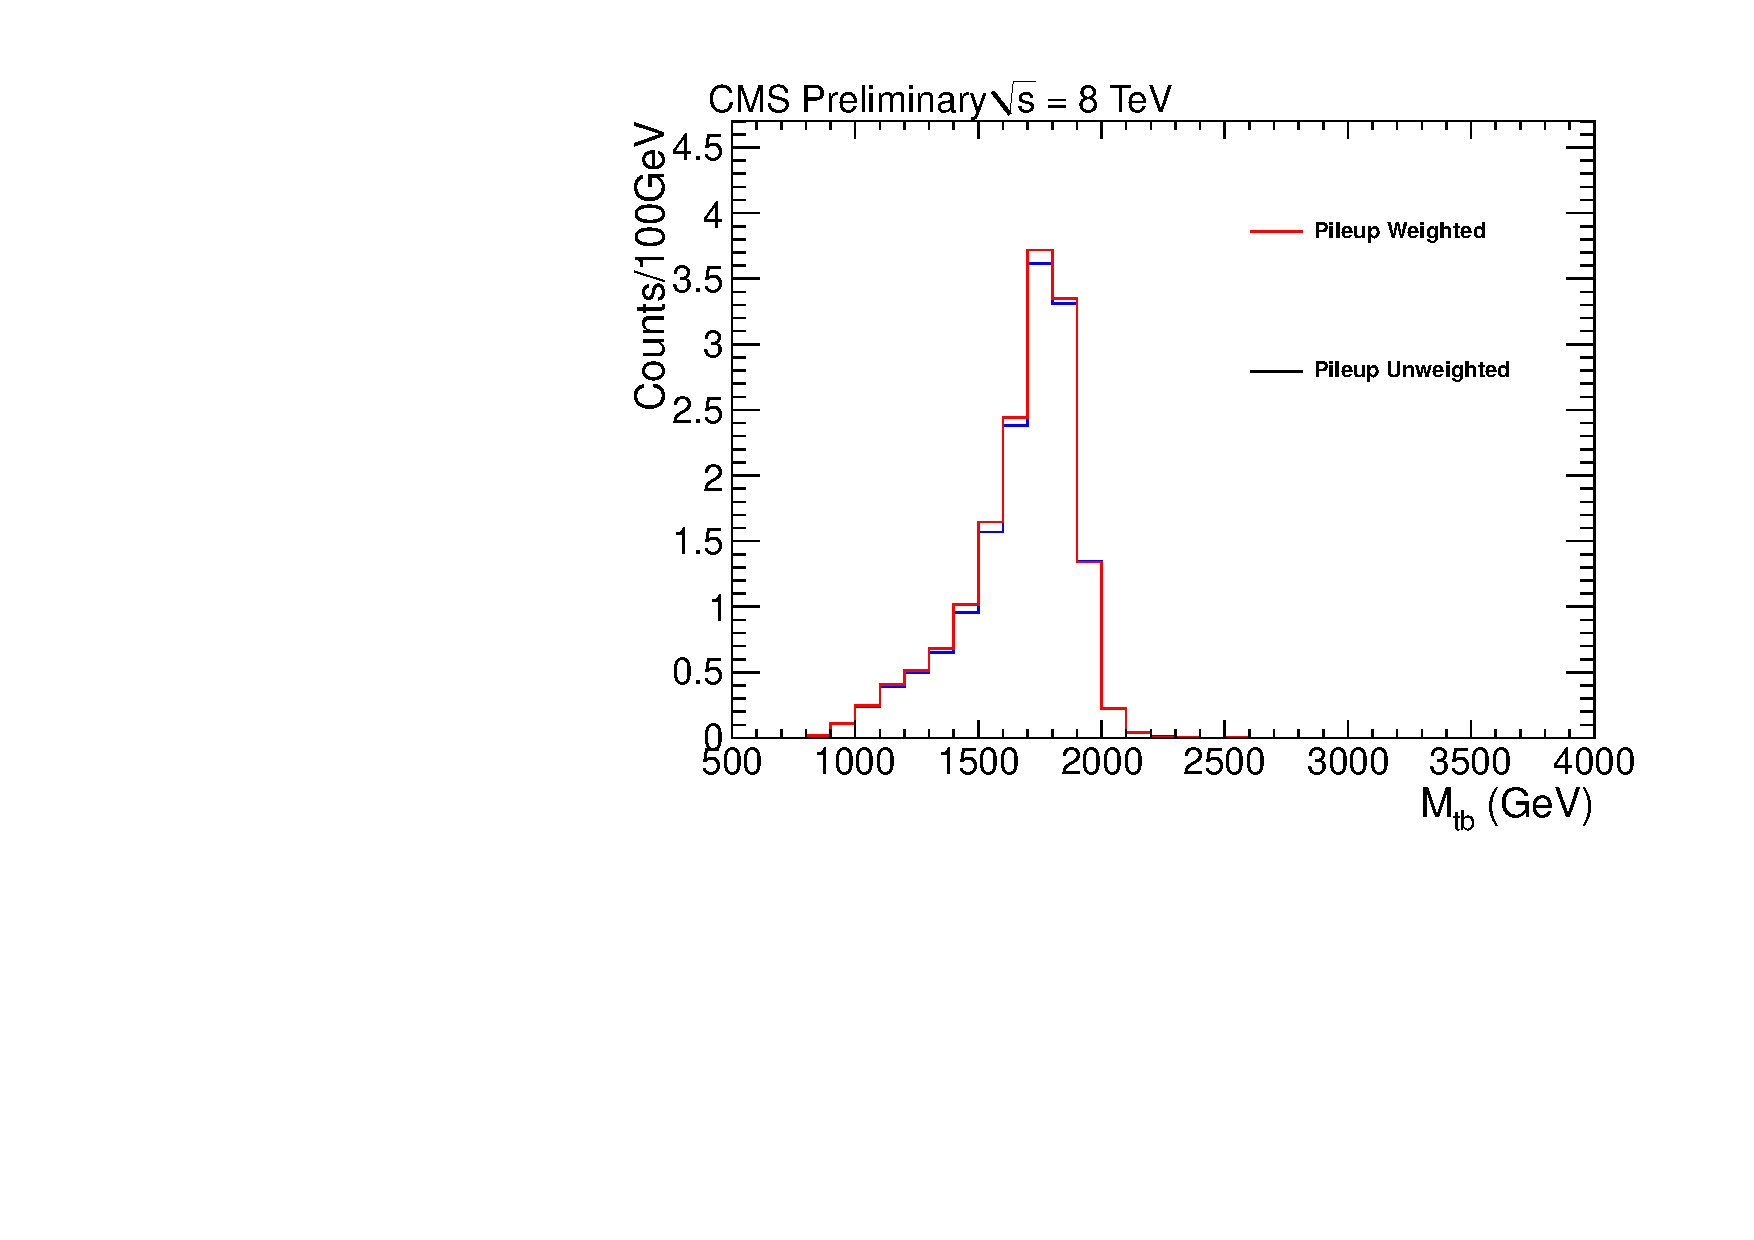
\includegraphics[width=0.9\textwidth]{AN-13-004/figs/Signal_M1900_PileupComp.pdf}
\caption{Effect of pileup-re-weighting on the Signal Monte Carlo.}
\label{figs:pileup3}
\end{figure}

\begin{figure}[htcb]
\centering
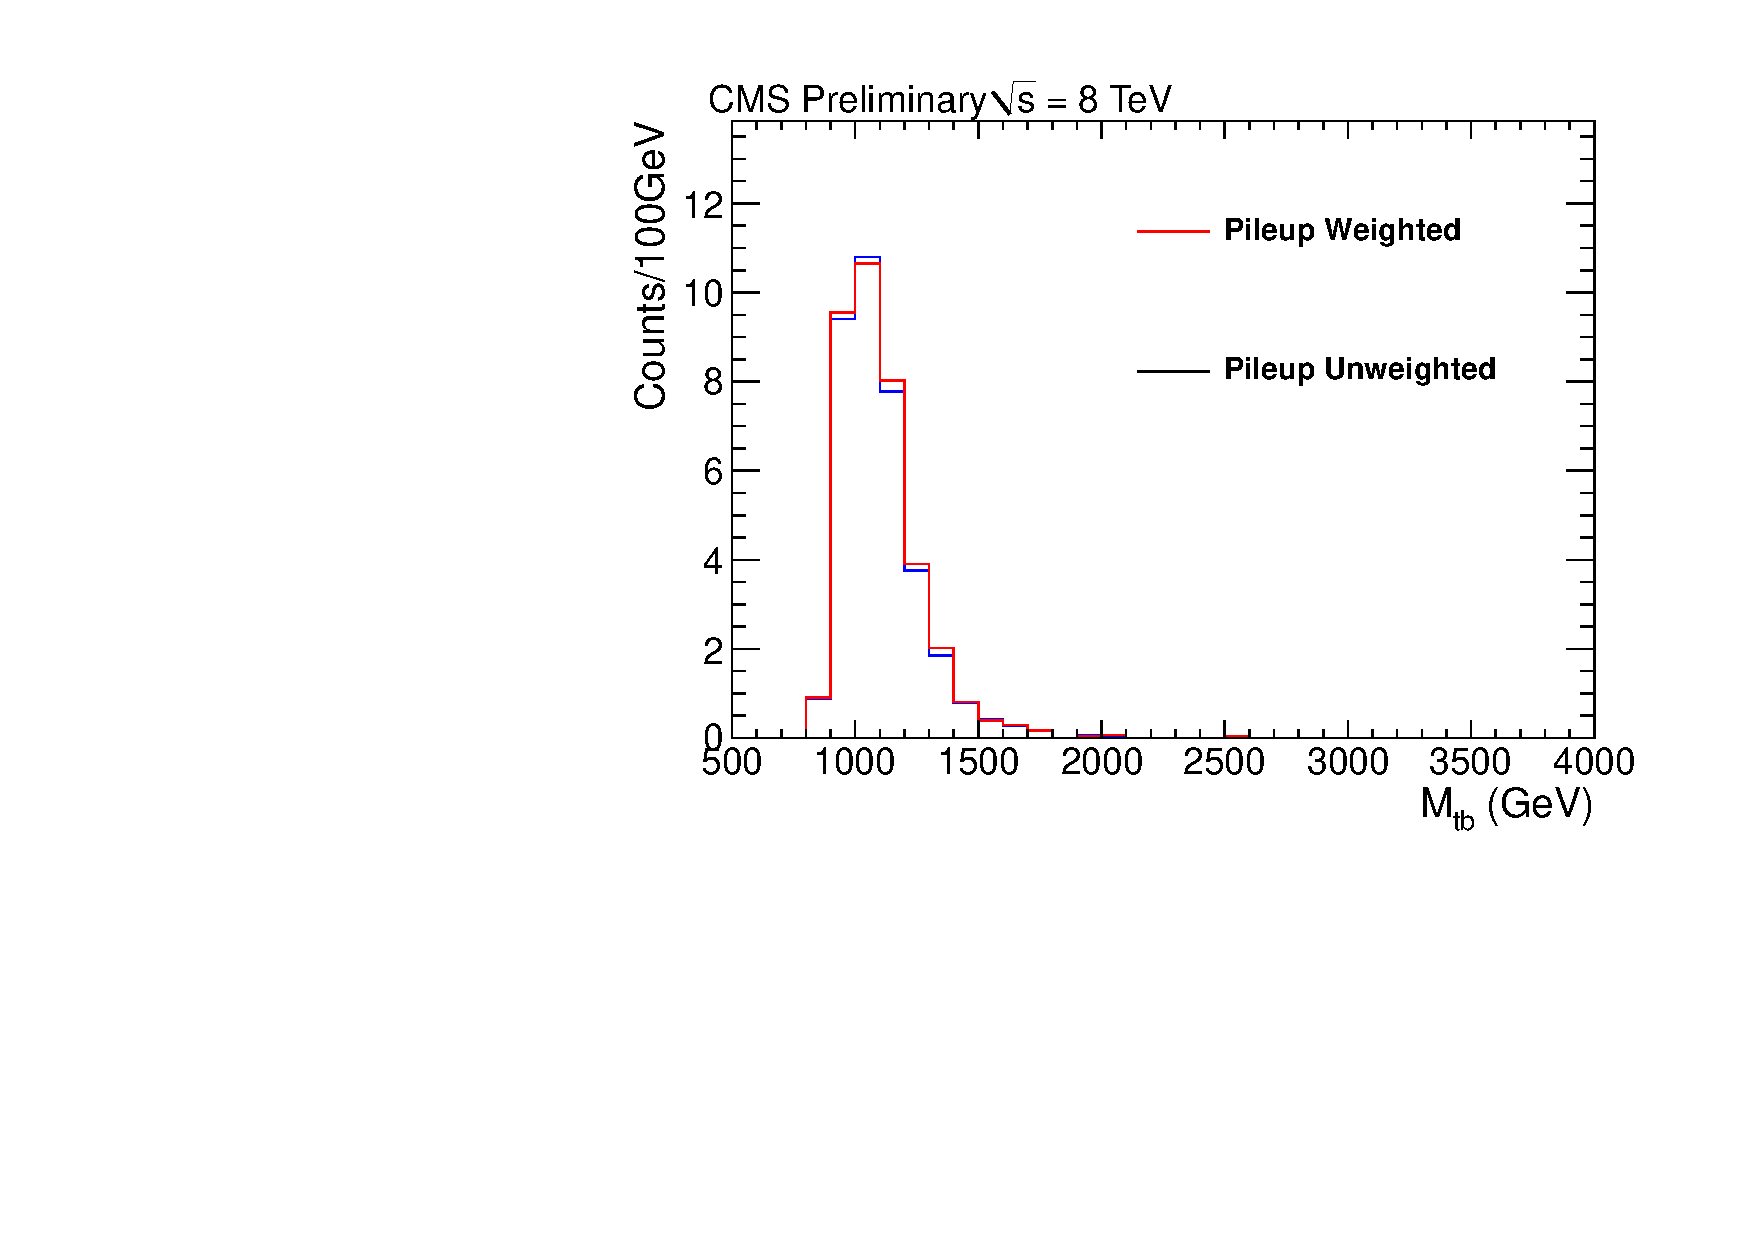
\includegraphics[width=0.9\textwidth]{AN-13-004/figs/TTbar_PileupComp.pdf}
\caption{Effect of pileup-re-weighting on the $\ttbar$ Monte Carlo.}
\label{figs:pileup3ttbar}
\end{figure}



\section{Combined CMS Top Tagging Algorithm}
\label{sec:toptagging}
\label{sec:subjetSF}

The CMS top tagging algorithm takes CA jets with $R = 0.8$ as input.  
The algorithm first attempts to decompose the CA jet into two primary subjets, and then 
performs a secondary decomposition to attempt to split the subjets into secondary subjets \cite{JME13007}.
In this process, particles with low $\pt$ or a large angular distance from the jet center are omitted.
The top tagging algorithm is based on the following cuts

\begin{itemize}
\item {\bf Jet Mass}  $\mathrm{\boldmath 140~\GeV < m_{\text{jet}} < 250~\GeV}$ - The mass of the CA jet is required to be consistent with the top quark mass. 
\item {\bf Number of Subjets}  $\mathrm{\boldmath N_{\text{subjets}} > 2}$ - The number of subjets found by the algorithm must be at least 3.
\item {\bf Minimum Pairwise Mass} $\mathrm{\boldmath m_{\text{min}} > 50~\GeV}$  - The three highest $\pt$ subjets are
taken pairwise, and each pair's invariant mass is calculated. $m_{\text{min}}$ is the mass of the pair with the lowest invariant mass. The minimum pairwise mass must be close to the W mass.   
\end{itemize}
Figure \ref{figs:CutCompP} shows the comparison of Signal and QCD Monte Carlo for the above top tagging selection. Here, the N-subjettiness and subjet b-tagging cuts are not applied.

\begin{figure}[htb]
\centering
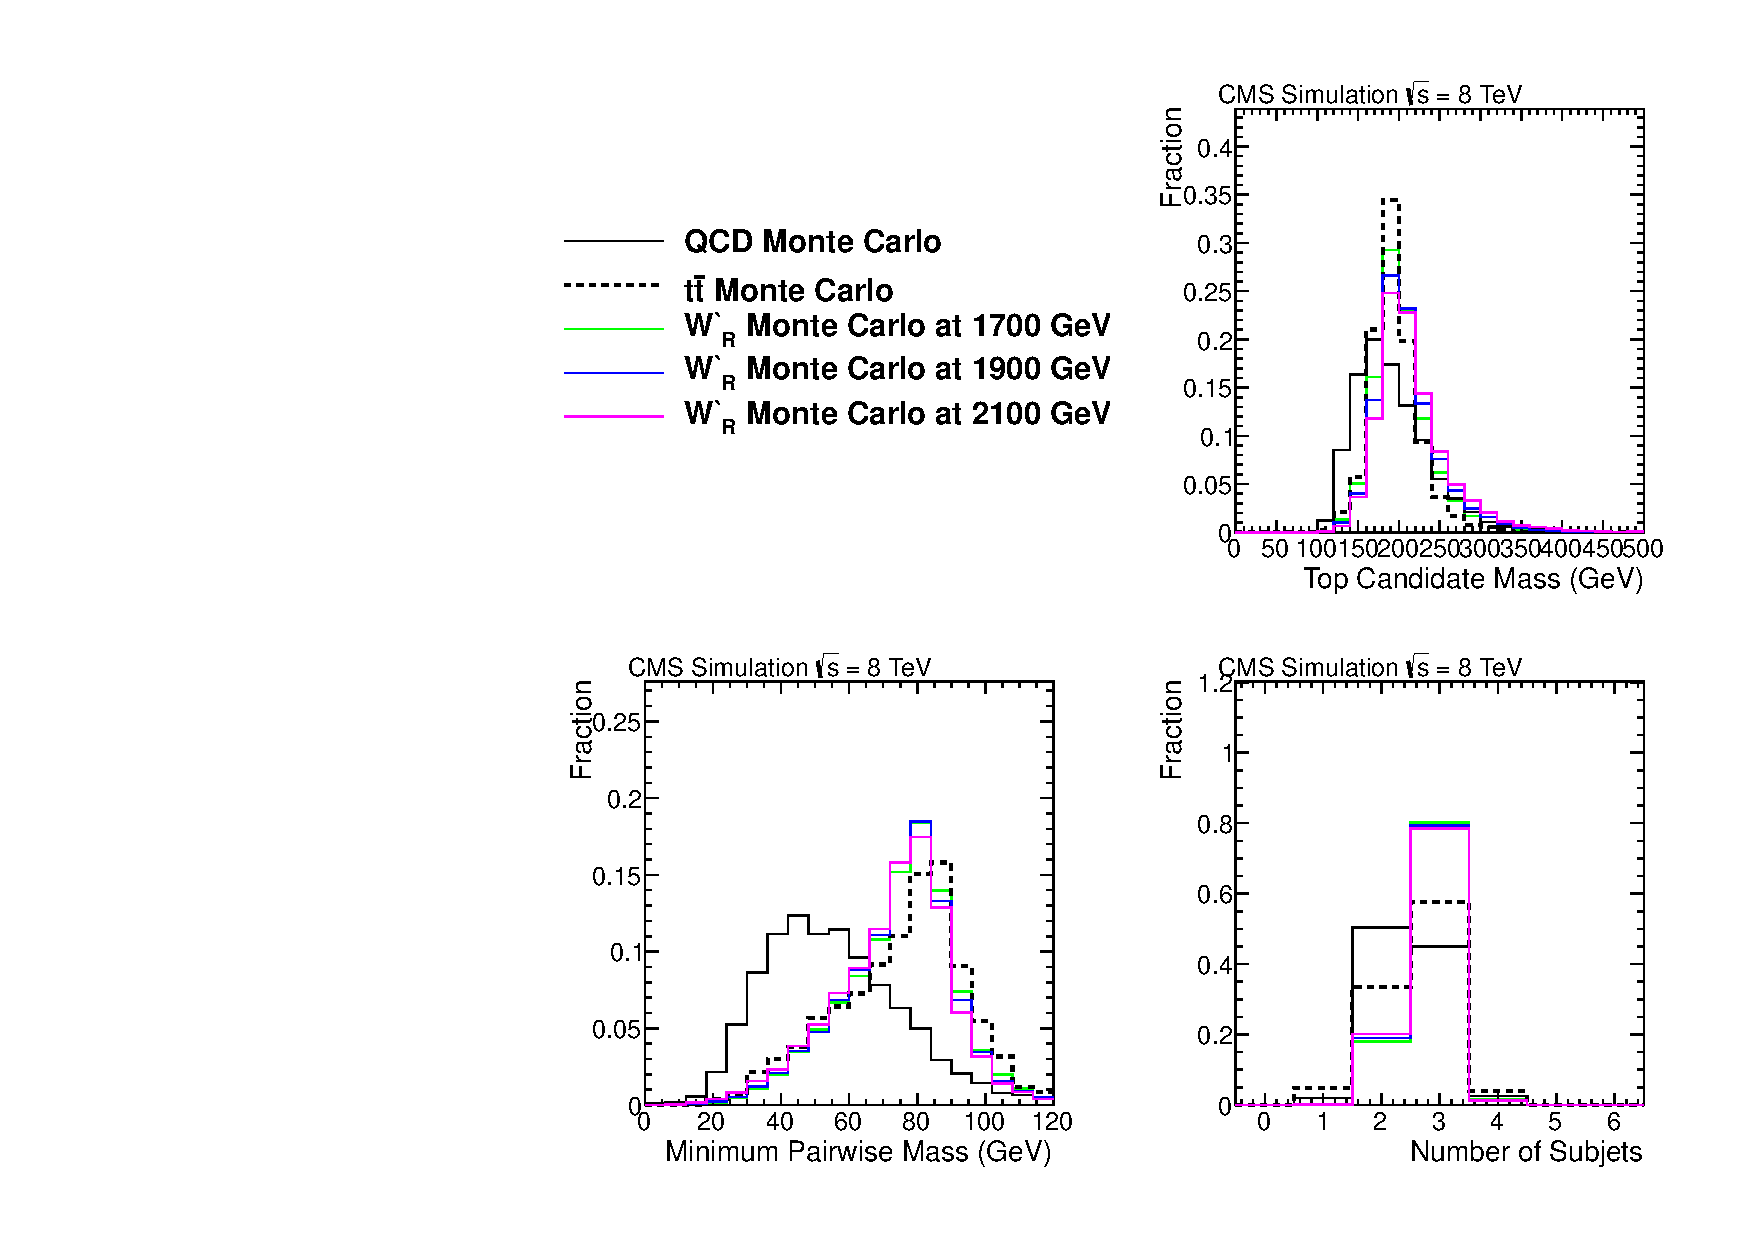
\includegraphics[width=1.0\textwidth]{AN-13-004/figs/CutCompqcdandsignal}
\caption{Comparison of the top Jet Mass, Number of Subjets, and Minimum Pairwise Mass in Signal and QCD Monte Carlo.  The cms top tagging selection is applied 
with the exception of the variable being plotted.}
\label{figs:CutCompP}
\end{figure}

The N-subjettiness algorithm can be used for boosted top jet identification \cite{Thaler:2011gf}.  N-subjettiness defines $\tau_N$ variables as follows 
\begin{eqnarray}
	\tau_{N} = \frac{1}{d_0}\sum_{i}p_{T_i}min\{\Delta R_{1,i},\Delta R_{2,i},...,\Delta R_{N,i}\}
\end{eqnarray}
where $\Delta R_{J,i}$ is between the subjet candidate and a constituent particle.  $d_0$ is a normalization factor 
\begin{eqnarray}
	d_0 = \sum_i p_{T_i} R_0
\end{eqnarray}
where $R_0$ is the characteristic jet radius used by the jet clustering algorithm.  For this analysis we use the one pass kt method of subjet axes minimization.  $\tau_N$ is a measure of how consistent the jet energy is with originating from N subjets. 
Additional discrimination power when using N-subjettiness variables is achieved by cutting on the ratio of two of these variables.   
Figure \ref{figs:NsubCOMP} shows $\tau_3/\tau_2$ comparison using signal and QCD Monte Carlo samples.  We use the standard operating point of $\tau_3/\tau_2 < 0.55$  \cite{JME13007} in the full selection.

\begin{figure}[htcb]
\begin{center}
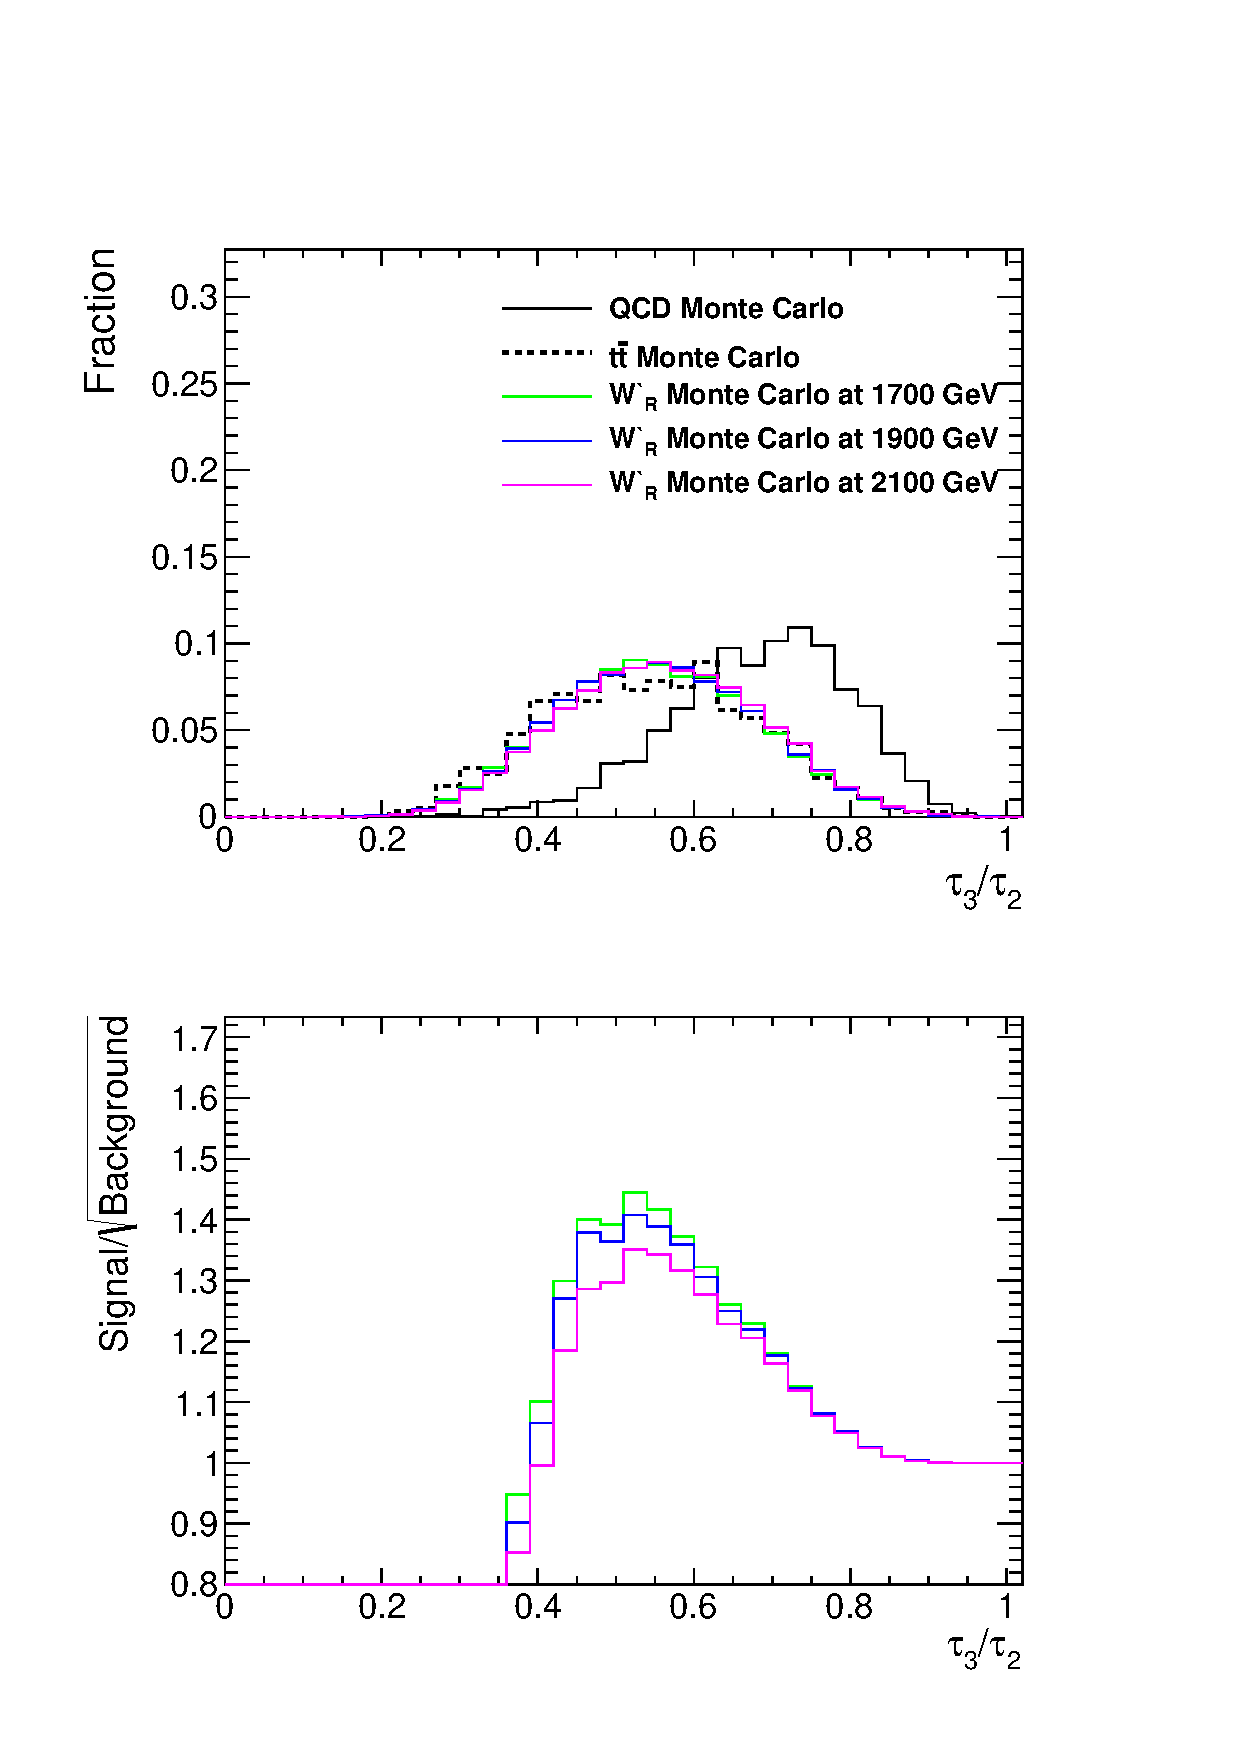
\includegraphics[width=0.7\textwidth]{AN-13-004/figs/tau32Compqcdandsignal.pdf}
\caption{
$\tau_3/\tau_2$ distributions in Signal and QCD Monte Carlo samples (top).  Plot of Signal/$\sqrt{\text{Background}}$ (bottom), derived from the top plot.
}
\label{figs:NsubCOMP}
\end{center}
\end{figure}

The use of b-tagging algorithms on subjets is described in \cite{CMS-PAS-BTV-13-001}.  We apply the Combined Secondary Vertex b-tagging algorithm 
to all of the subjets found by the CA declustering sequence described 
above.  The optimal discrimination variable when using subjet b-tagging is the maximum discriminant out of the three or four subjets found.  
Figure \ref{figs:BtagCOMP} shows the maximum subjet CSV b discriminant comparison using signal and QCD Monte Carlo samples.  We use the standard CSV working point $SJ_{\text{CSVMAX}} > 0.679$.

\begin{figure}[htcb]
\begin{center}
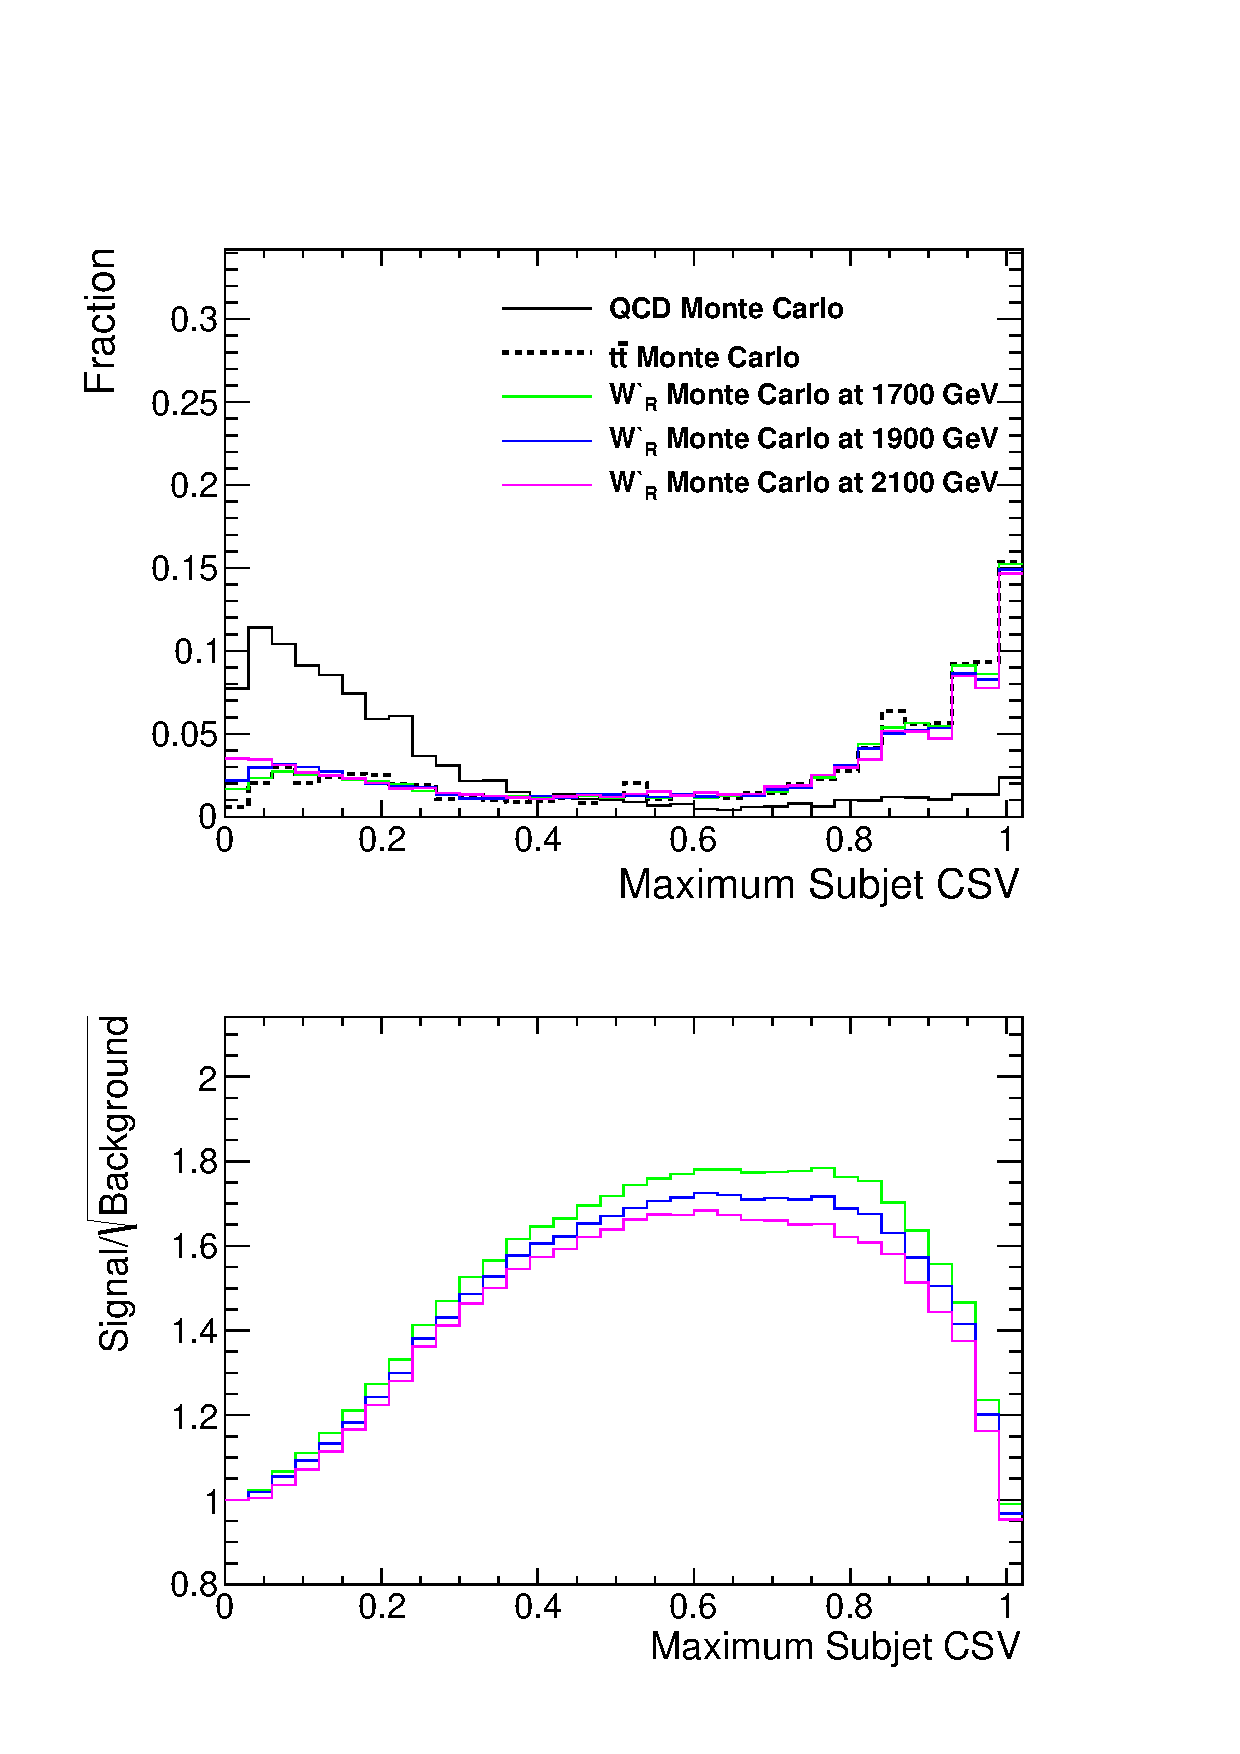
\includegraphics[width=0.7\textwidth]{AN-13-004/figs/bmaxCompqcdandsignal.pdf}
\caption{
Maximum subjet CSV distributions in Signal and QCD Monte Carlo samples (top).  Plot of Signal/$\sqrt{\text{Background}}$ (bottom), derived from the top plot. 
}
\label{figs:BtagCOMP}
\end{center}
\end{figure}

Substructure variables in the signal region have known differences in data and Monte Carlo \cite{JME13007}.  
We use the top tagging scale factor with the addition of subjet b-tagging and N-subjettiness discrimination that is extracted 
from efficiency comparisons of data and Monte Carlo in a highly pure semileptonic $\ttbar$ sample.   
The scale factor for this effect is 1.04 and is applied to the signal Monte Carlo samples used in the main analysis.  
There is a 13\% uncertainty on this scale factor which is purely statistical, as the study is dominated by statistical uncertainty.  
The scale factor is obtained from the plots shown in Figure \ref{figs:type1_topmasspowheg}.

\begin{figure}
\begin{center}
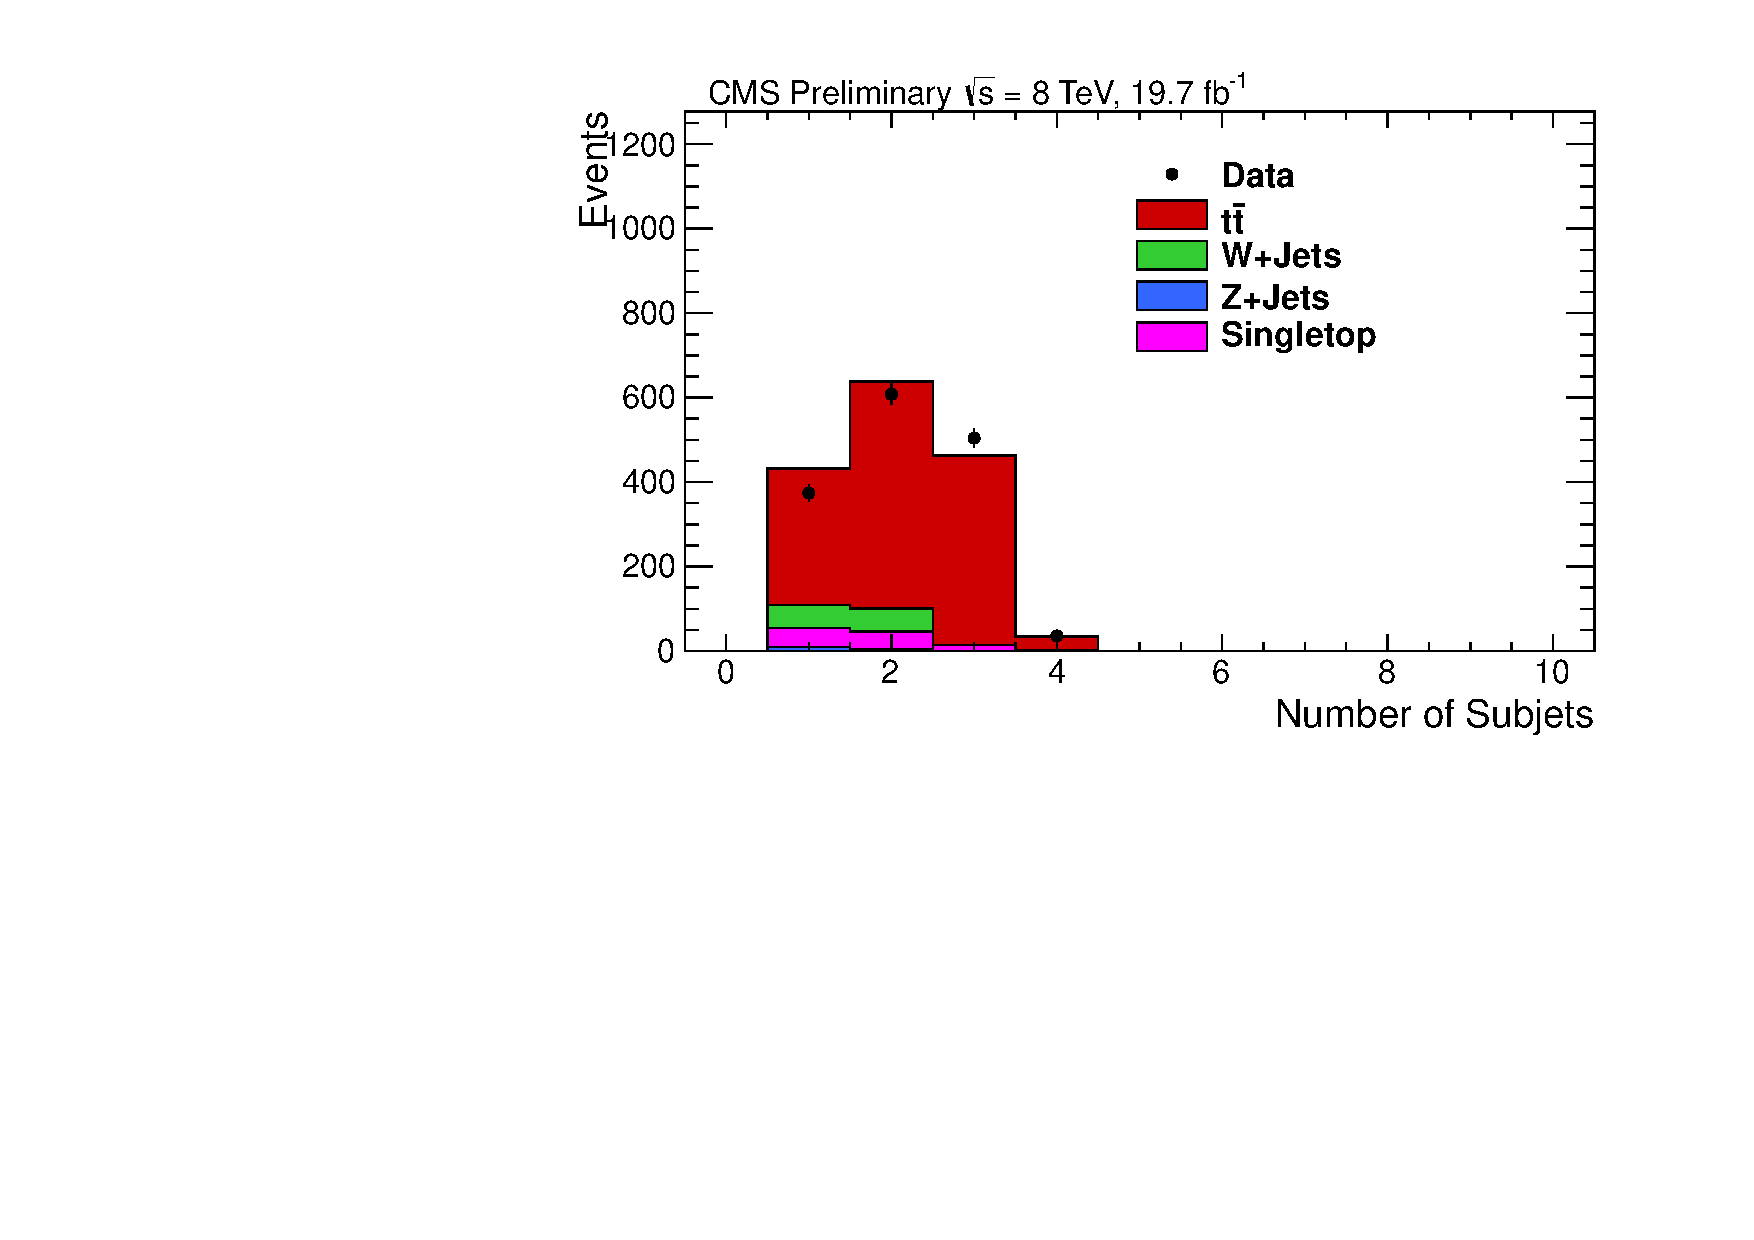
\includegraphics[width=0.45\linewidth]{AN-13-004/figs/semiLepMass_t1Nsubjets_POWHEG_TTWeight.pdf}
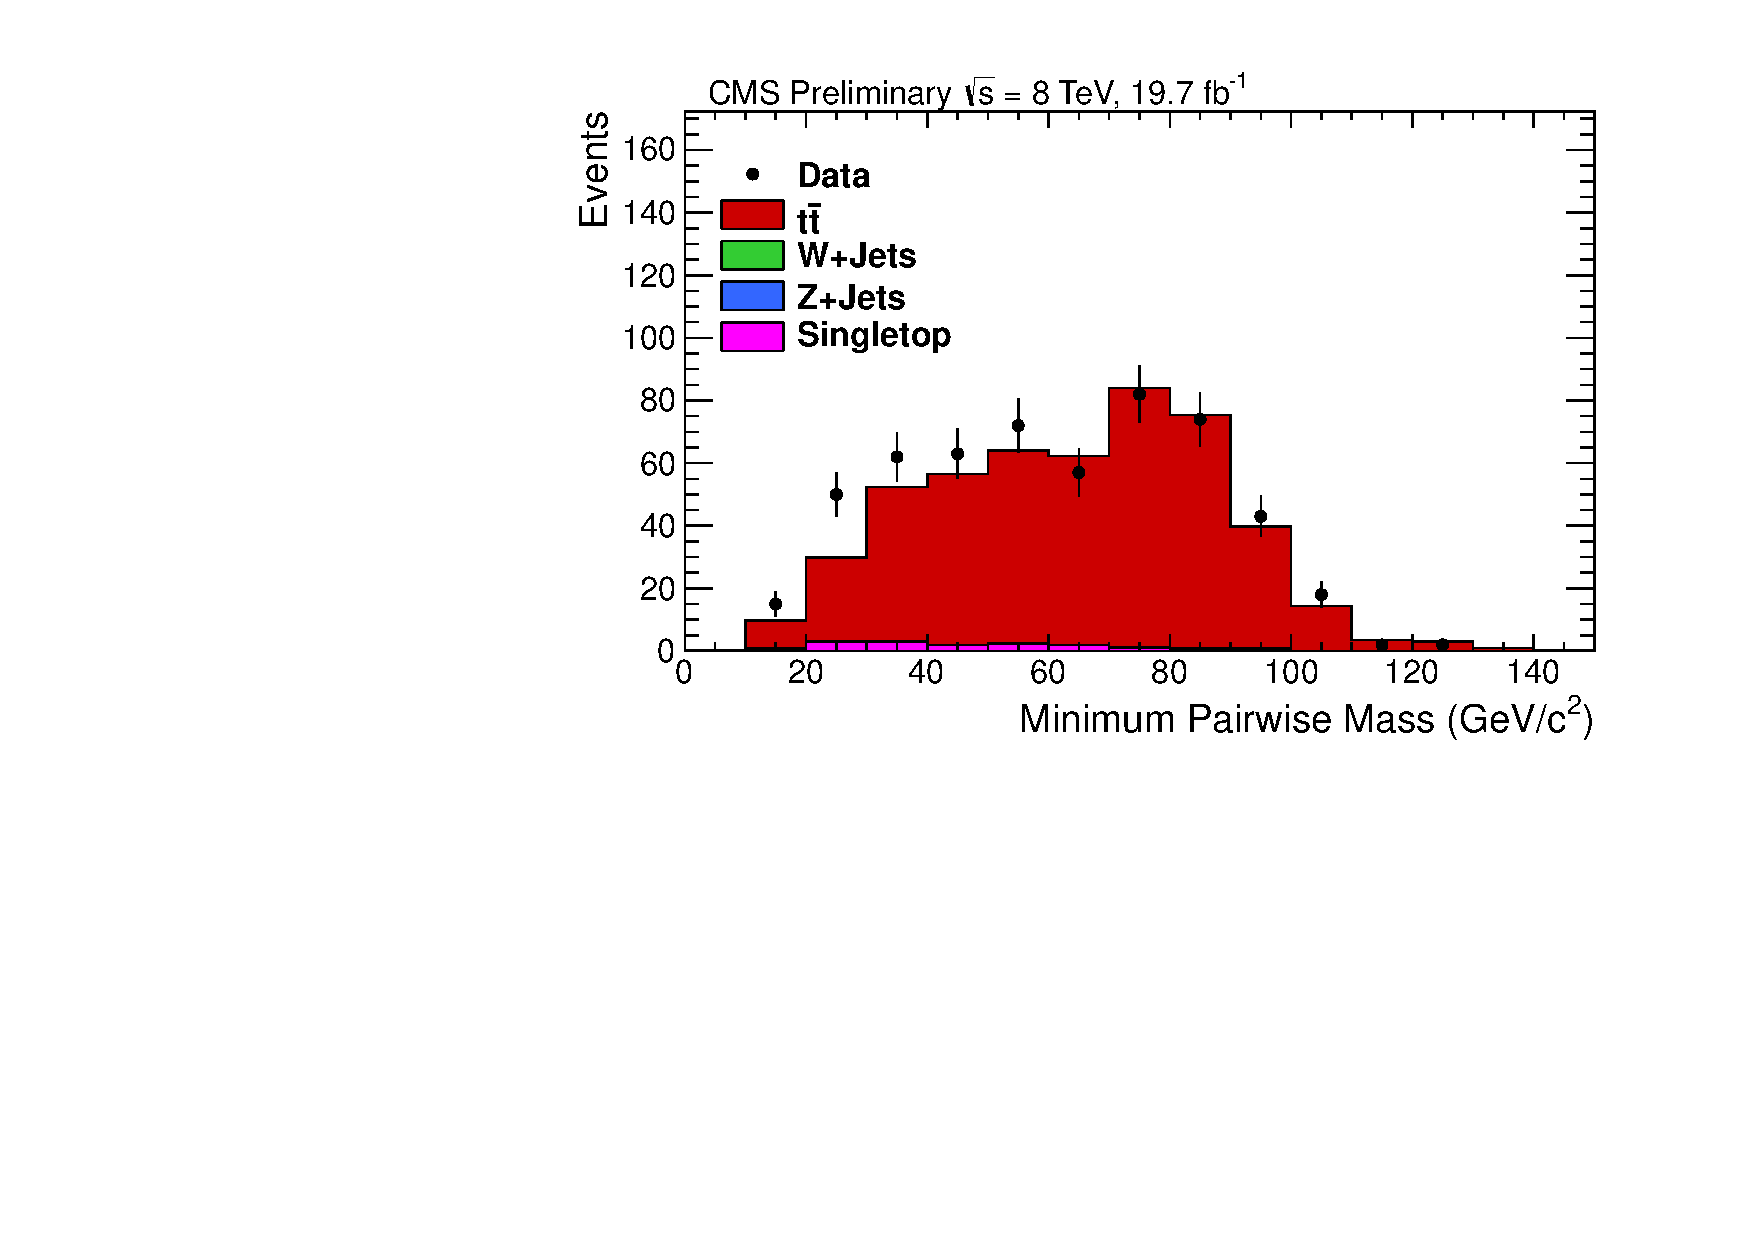
\includegraphics[width=0.45\linewidth]{AN-13-004/figs/semiLepMass_t1MinimumPairwiseMass_POWHEG_TTWeight.pdf}\\
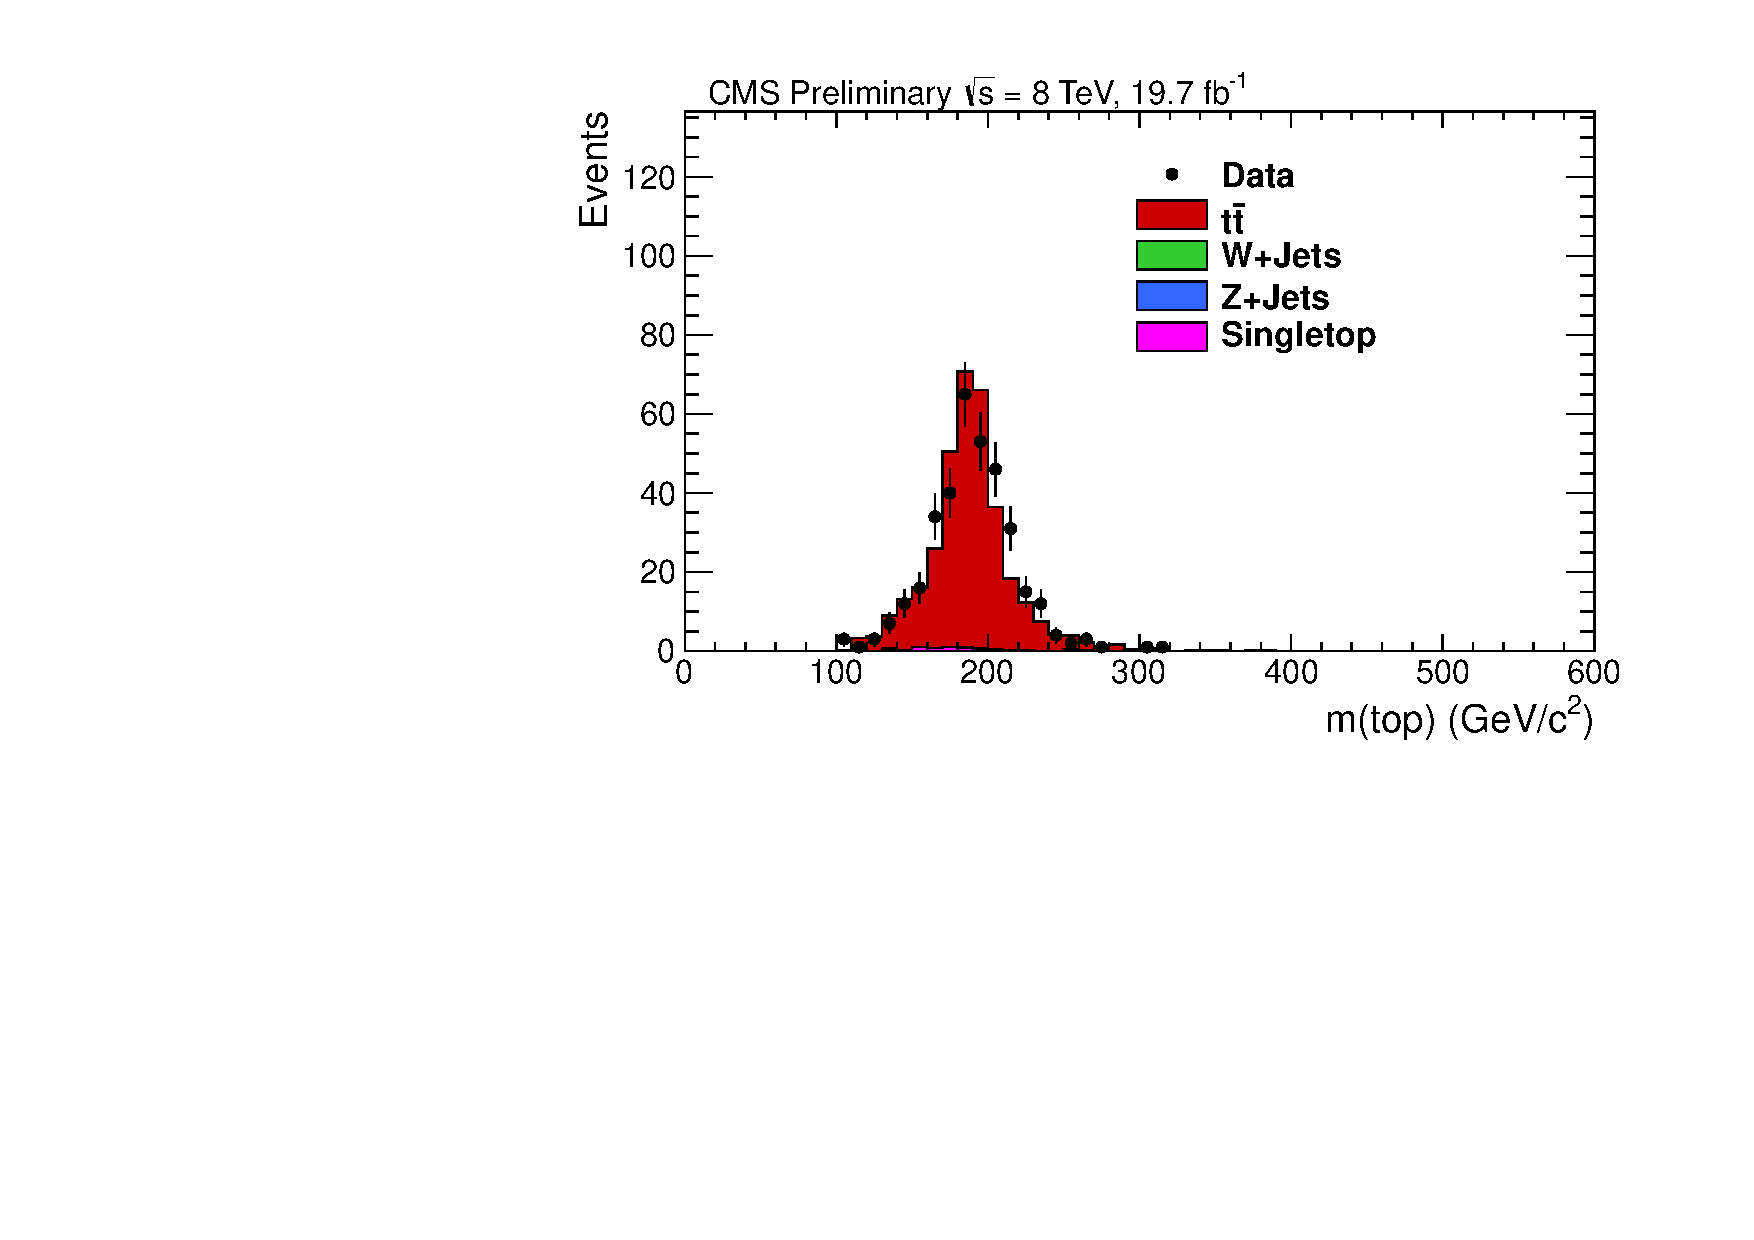
\includegraphics[width=0.45\linewidth]{AN-13-004/figs/semiLepMass_t1TopMass_POWHEG_TTWeight.pdf}
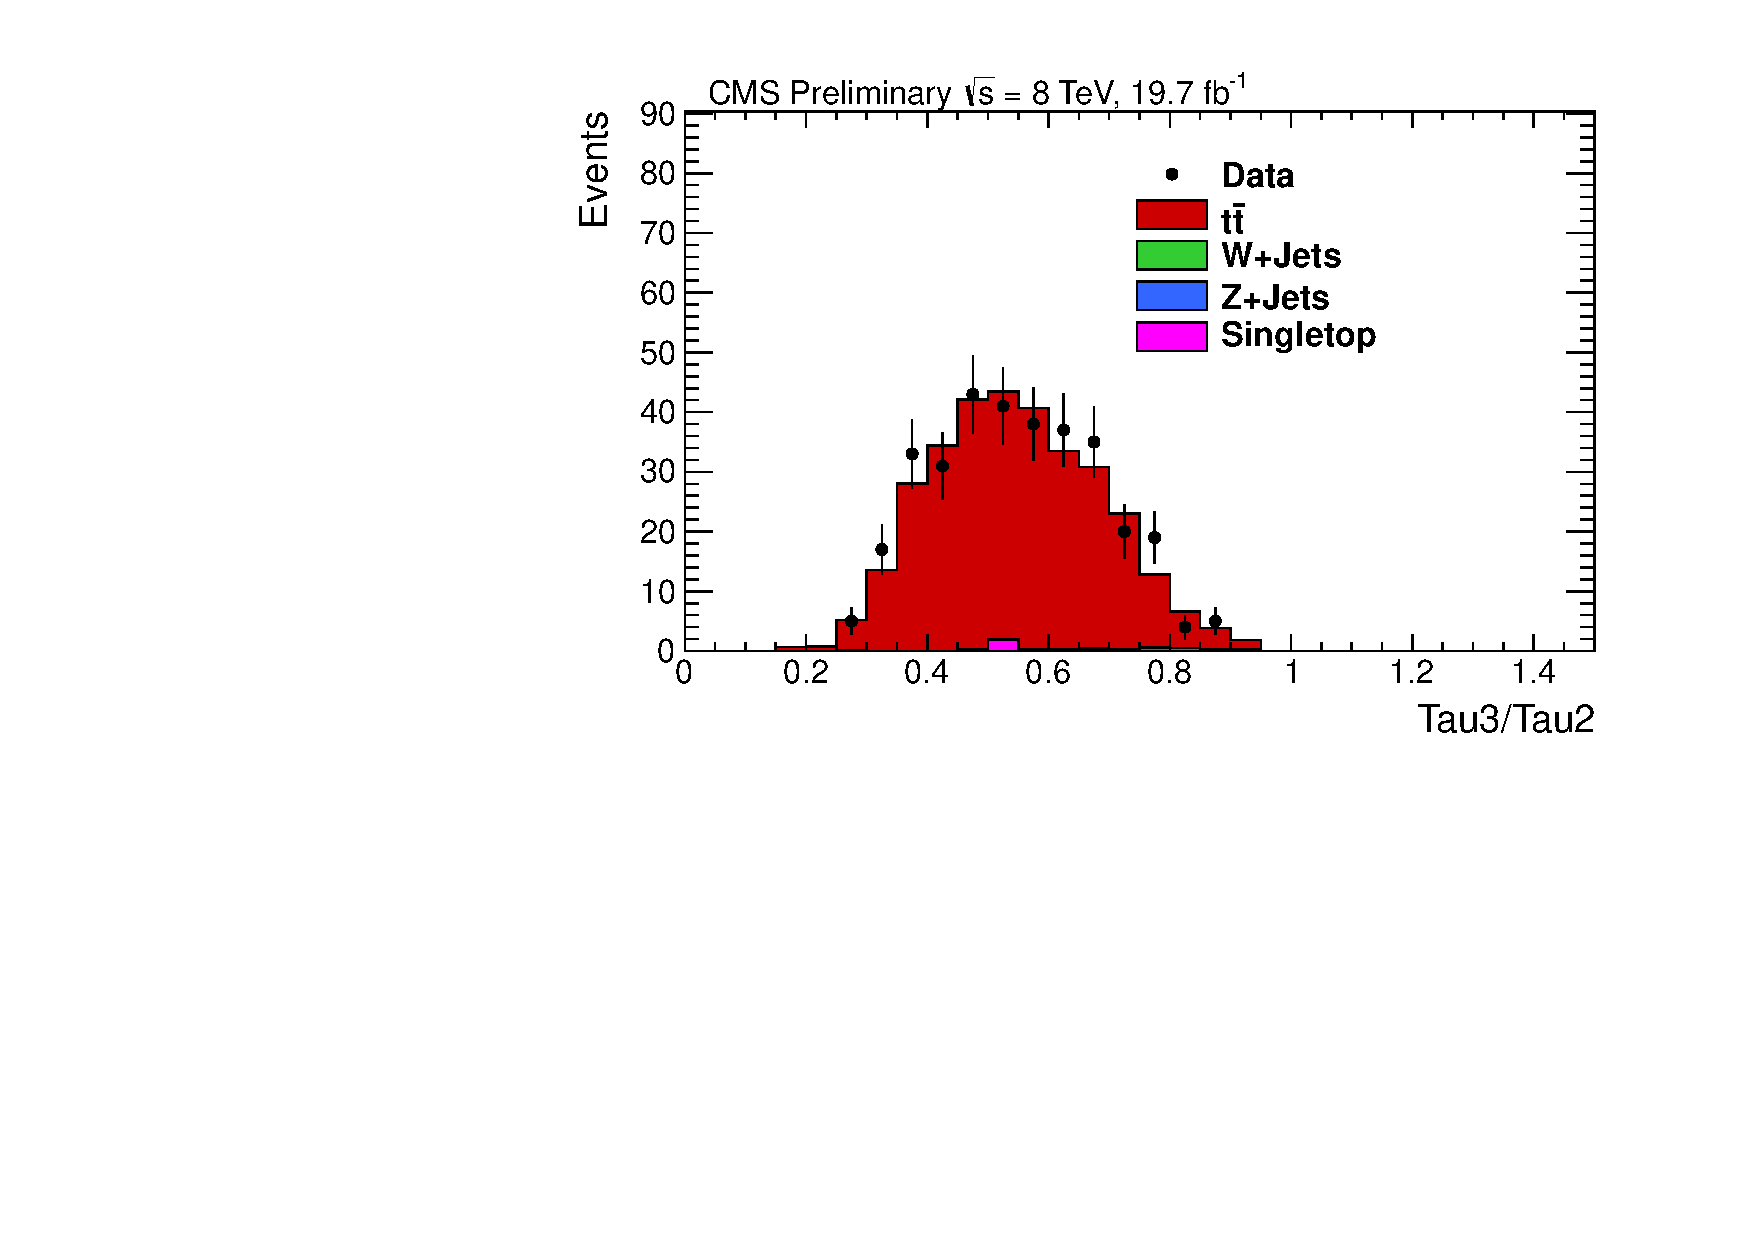
\includegraphics[width=0.45\linewidth]{AN-13-004/figs/semiLepMass_t1Tau32_POWHEG_TTWeight.pdf}\\
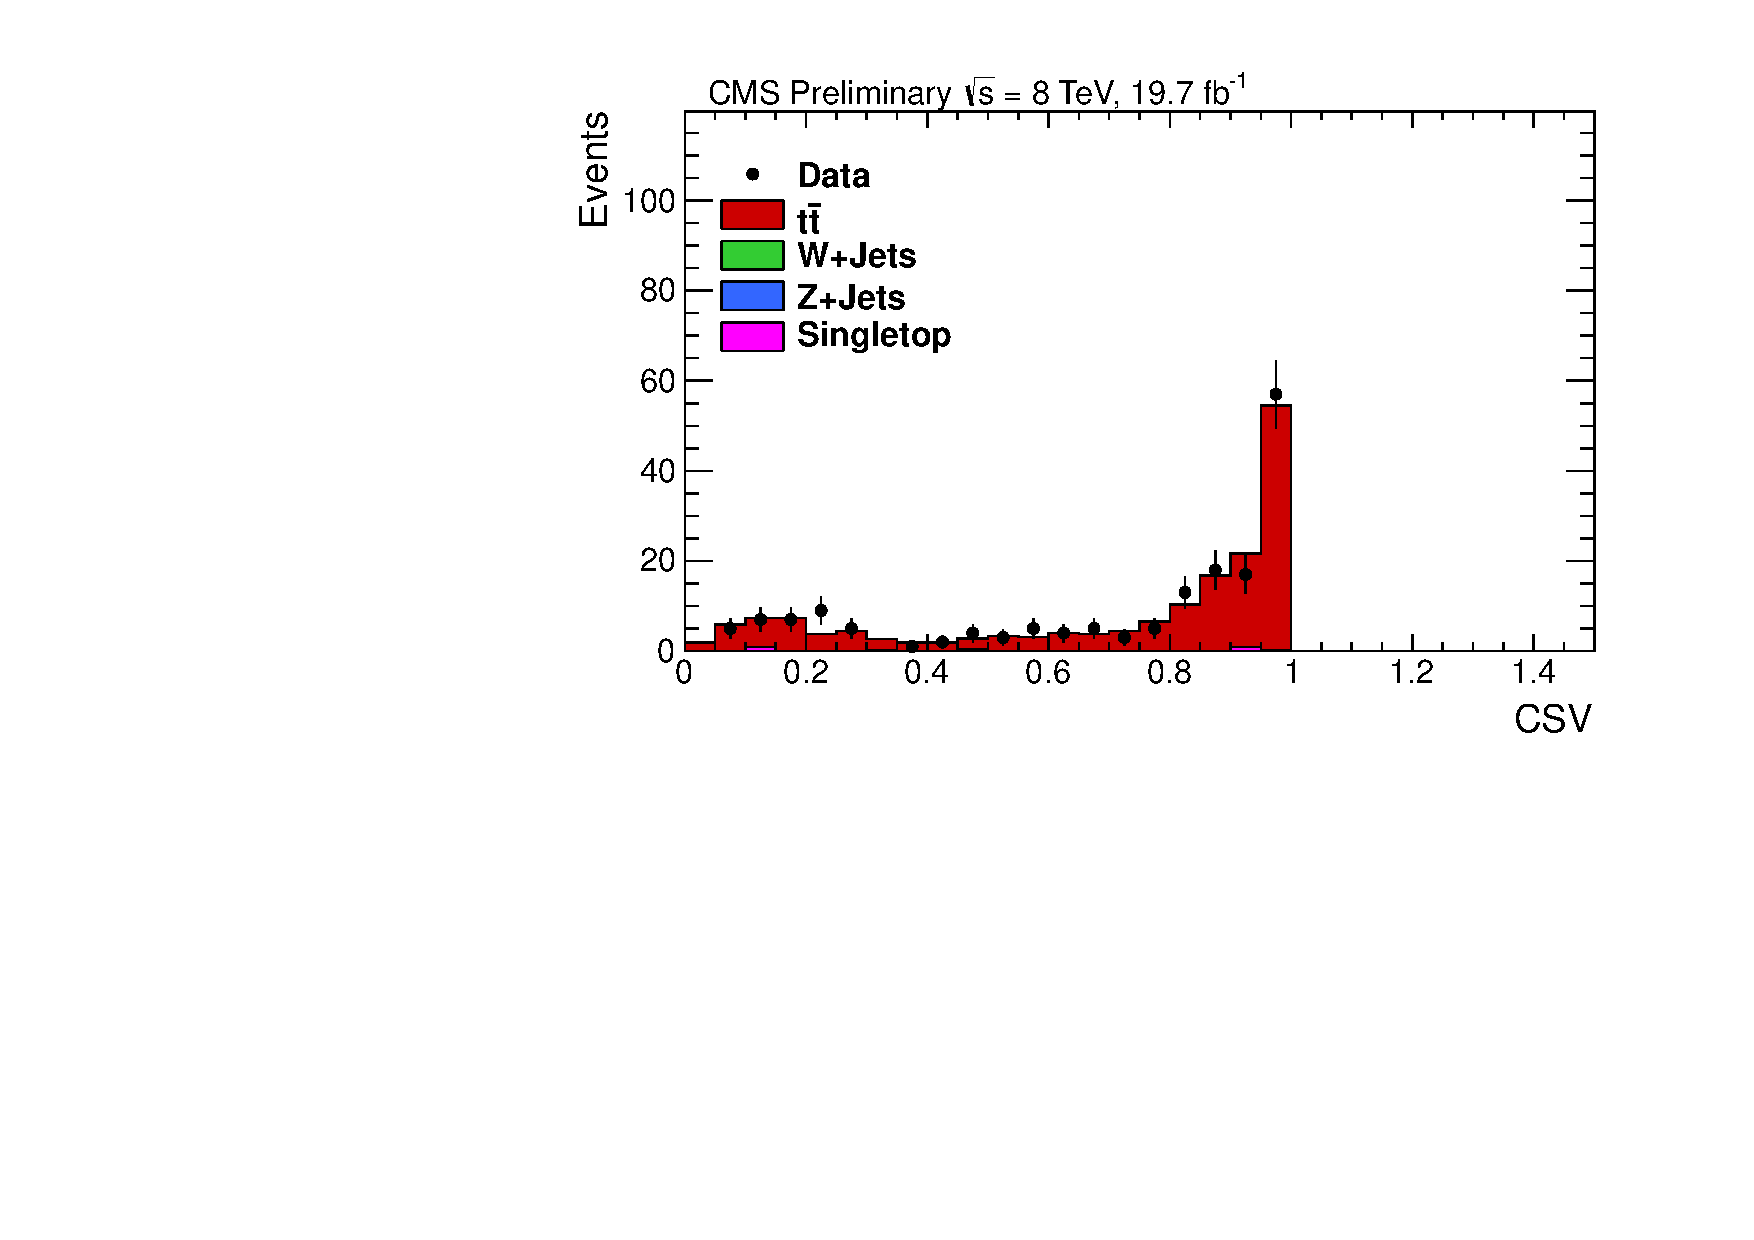
\includegraphics[width=0.45\linewidth]{AN-13-004/figs/semiLepMass_t1BMax_POWHEG_TTWeight.pdf}
\end{center}
\caption{ a.)Number of subjets, b.)minimum pairwise subjet mass, c.)jet mass, d.)$\tau_{3}/\tau_{2}$, and  e.)maximum subjet CSV for fully-merged top candidates
  found in the semileptonic $\ttbar$ sample, used to evaluate the top-tagging efficiency SF.  These Figures are extracted using the Powheg $\ttbar$ Monte Carlo Sample. }%  The shaded regions represent the total uncertainty on the background model.}
\label{figs:type1_topmasspowheg}
\end{figure}

\section{Delta Rapidity Cut}
\label{sec:deltarapidity}
At high $M_{\tbbar}$, jets that originate from QCD multijet production are widely separated in rapidity (high $\Delta y$).
However the jets originating from a high mass $\tbbar$ resonance do not exhibit such pronounced separation.  The effect is not pronounced over the entire 
$M_{\tbbar}$ spectrum, but for high values of $M_{\tbbar}$ the analysis can achieve greater separation of signal and background.  We therefore place a cut on $|\Delta y| < 1.6$ 
for the full selection.  The value for this cut was chosen by investigating the Signal/$\sqrt{\text{Background}}$ distribution in events that have $M_{\tbbar}>2000~\GeV$.  
Because it is not as effective over the entire $M_{\tbbar}$ range, the value is set slightly off the peak to minimize loss of signal efficiency.
%The value of 1.6 was determined by optimizing $S/\sqrt{B}$ where $S$ is the number of events in the signal region and $B$ is the number of events attributed to background in the region of interest for each signal mass point.  The cut value was chosen based on maximizing the expected counting experiment limit described in Section \ref{sec:countingexperiment}.  
Figure \ref{figs:CutComp} shows the comparison of $|\Delta y|$ for high $M_{\tbbar}$ in signal and QCD MC.  
Here, the N-subjettiness and subjet b-tagging cuts are not applied.
% Additionally, the lowest $\pt$ QCD MC sample has poor statistics for the high $M_{tb}$ region and is not included in this figure.

\begin{figure}[htb]
\centering
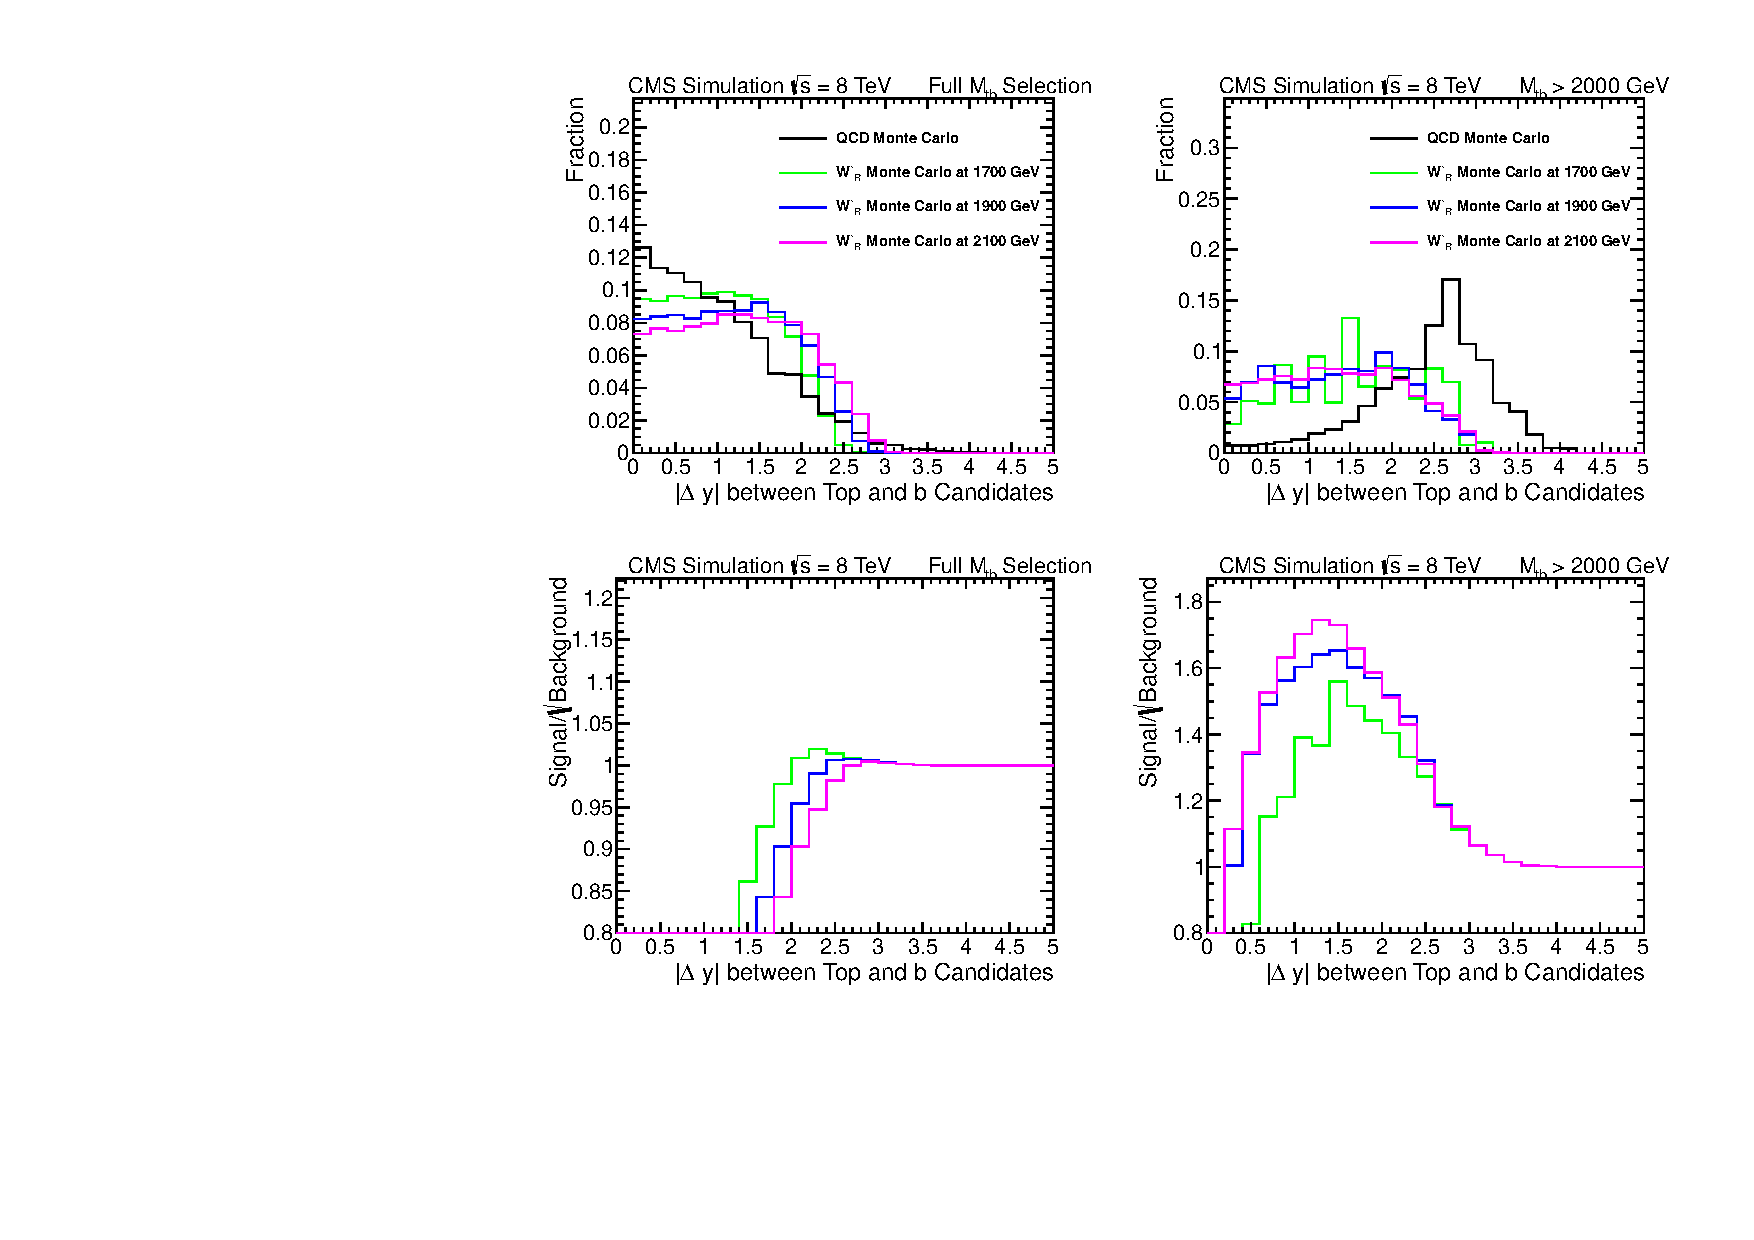
\includegraphics[width=1.0\textwidth]{AN-13-004/figs/drapCompqcdandsignal}
\caption{Comparison of $|\Delta y|$ in signal and QCD Monte Carlo for the full selection and only events with $M_{\tbbar} > 2000~\GeV$}
\label{figs:CutComp}
\end{figure}



\section{b-jet Identification}
\label{sec:btagging}
To enhance the sensitivity of the analysis, the Combined Secondary Vertex (CSV) b-tagging algorithm is applied to the subleading jet. We use the standard operating point CSVM (CSV $>$ 0.679).
%after optimizing S/$\sqrt{B}$ using all 8TeV supported b-tagging algorithms and operating points.  
Due to the fact that our signal content 
contains only $\tbbar$ and the only Monte Carlo used in background estimation is $\ttbar$, the Monte Carlo to data scale factor used in the analysis for b-tagging 
is the b-tagging Scale Factor for b quarks ($SF_b$).  We use the suggested scale factor parameterized in $\pt$ with the following functional form for 
b candidate jet $\pt < 800~\GeV$

\begin{eqnarray}
SF_b = 0.938887 + 0.00017124\times \pt - 2.76366 \times 10^{-07} \times \pt^2 
\end{eqnarray}
Any b candidate jet with $\pt > 800~\GeV$ is weighted with $SF_b$ evaluated at 800$~\GeV$.  The parameterized $SF_b$ is the 
suggested EPS13 prescription \cite{CMS-PAS-BTV-13-001} from the b-tagging POG generated from measurements in both muon-jet and ttbar data representing 20$~\fbinv$ of integrated 
luminosity. The uncertainty associated with this scale factor parameterization is described in Chapter \ref{sec:systematics}.  b-tagging operating points 
and scale factors have been validated for use with anti-kt jets with a R value of 0.5 (AK5 jets).  In our kinematic regime it is assumed that the change in cone size 
will have a small effect. We apply an additional $2\%$ systematic uncertainty to the signal Monte Carlo samples used in the analysis. This is a conservative estimate of the uncertainty, validated by the following study: 

For the $2700~\GeV$ signal sample, we 
included both AK5 and CA8 jets in the event selection.  All jets considered were required to be in our pt range ($\pt > 350~\GeV$).  We attempt to match a CA8 jet to 
the corresponding AK5 jet using a constraint on $\eta$ and $\phi$ ($\Delta$R $< 0.3$ ).  The results were 579041 CA8 jets pass pt cut,
of these, 567155 pass the $\eta$ , $\phi$ matching to AK5 jets.  Of the matched jets, $96.9\%$ record the same value for the CSVM cut (pass or fail). In addition, 
the ratio of b-tagging efficiencies for both AK5 and CA8 were found to be within a $2\%$ deviation (see Figure \ref{figs:btageff}).  To rule out a bias based on the 
known differences in pt for CA8 and AK5 jets, the efficiencies and uncertainties were extracted from plots using only the pt of the CA8 jet.  
The fit on the b-tagging efficiency ratio for CA8 and AK5 jets can be interpreted as an upper bound on the uncertainty due to this effect.
We also checked this process for $1300~\GeV$ and $1900~\GeV$ signal samples and found results consistent with this $2\%$ error. 
We have verified this systematic uncertainty with the BTV group, and it is approved for use in our analysis.

\begin{figure}[htcb]
\centering
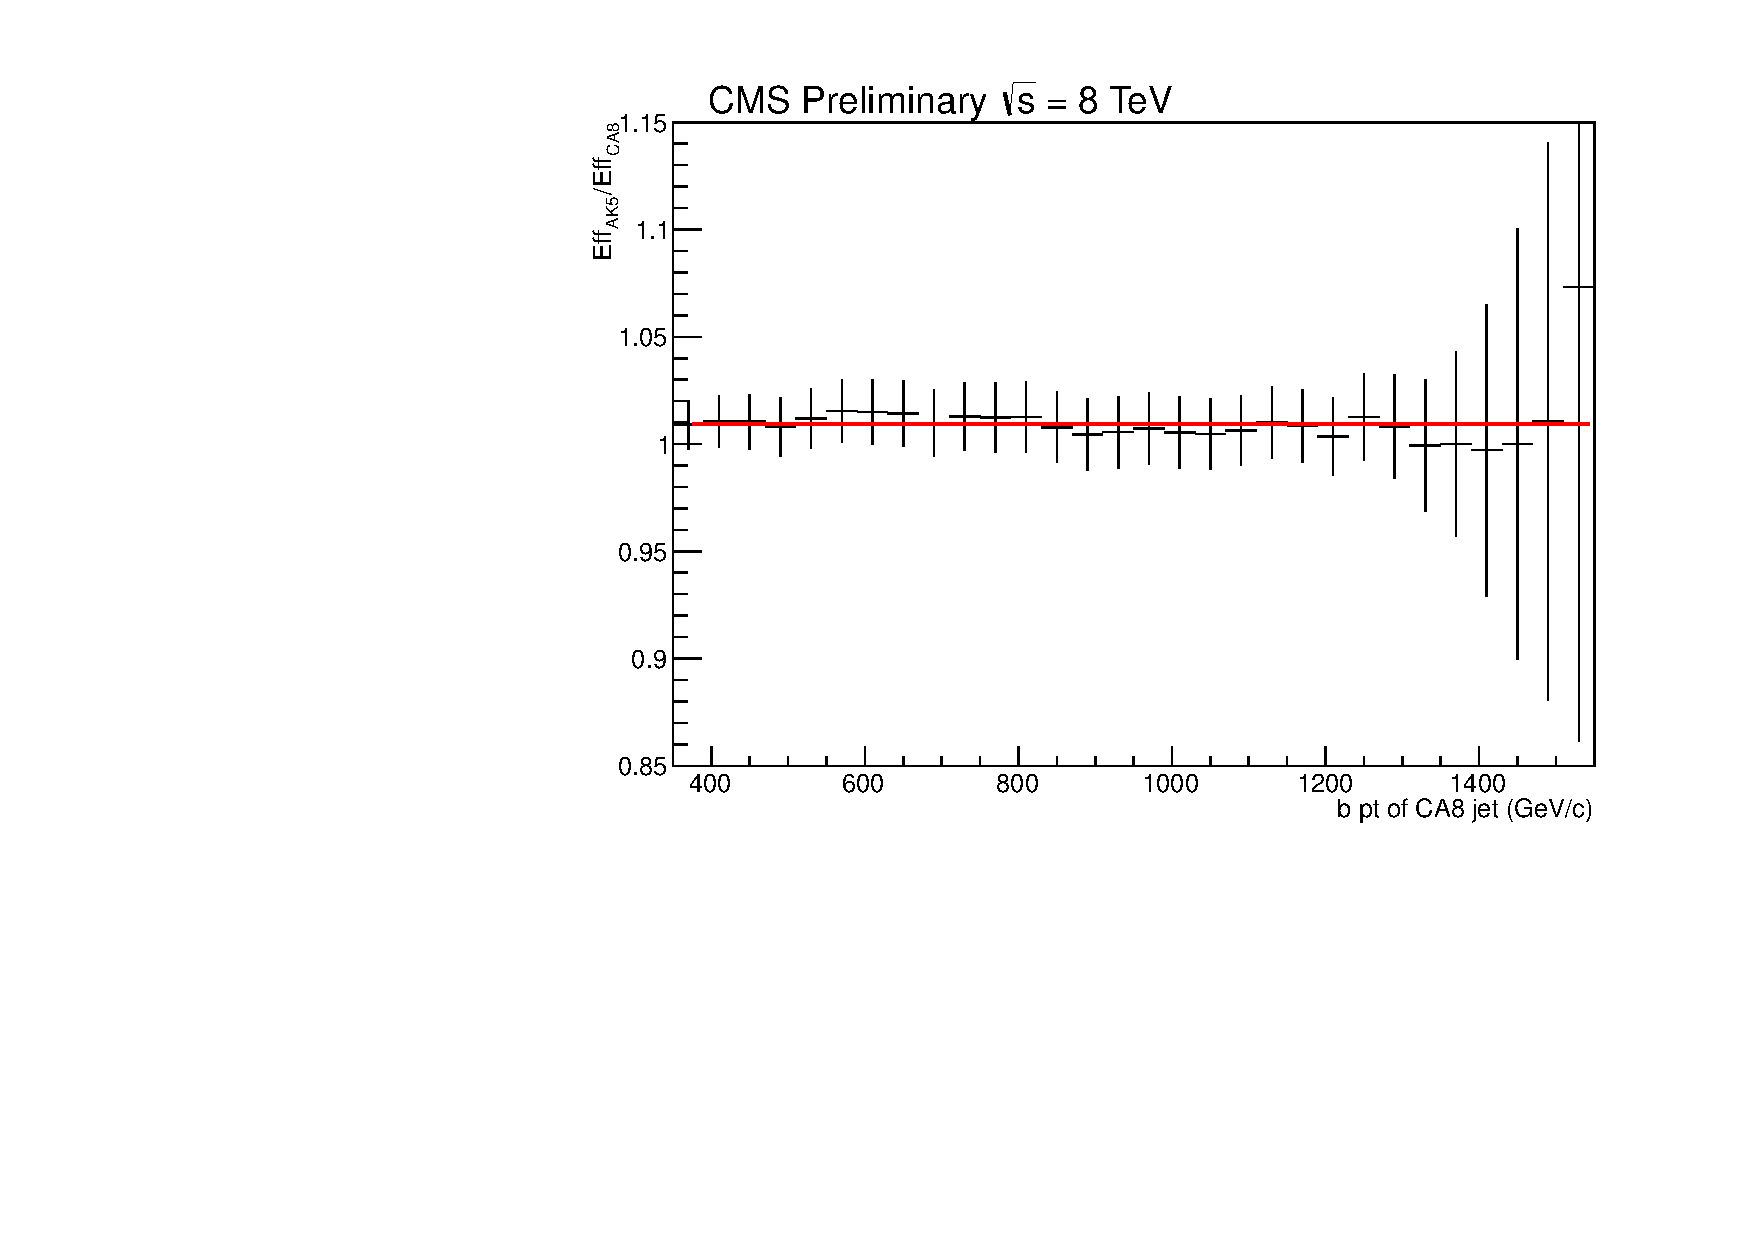
\includegraphics[width=0.9\textwidth]{AN-13-004/figs/EfficiencyCompCAptr32700.pdf}
\caption{Ratio of the AK5 b-tagging rate to the CA8 b-tagging rate. Fitting this to a constant gives us a value of 1.0098 $\pm$ 0.0031.  This can 
be considered an upper limit on the uncertainty for the change in $SF_b$ for CA8 jets}

\label{figs:btageff}
\end{figure}

After the full top tagging selection is complete, there is a substantial fraction of $\ttbar$ in the full selection.
Additionally, there is a large uncertainty in the $\ttbar$ Monte Carlo contribution, so discriminating signal from $\ttbar$ becomes important.  
In $\wpr$ signal Monte Carlo, the sub-leading b candidate jet is usually a true b jet, but in $\ttbar$ this jet is commonly a merged W or top jet. 
To this effect, the b candidate jet is required to have a mass $M_b < 70~\GeV$ in the full selection.  The value for this cut is set near the peak of the Signal/$\sqrt{\text{Background}}$ distribution (see Figure \ref{figs:BmassCOMP}).


\begin{figure}[htcb]
\begin{center}
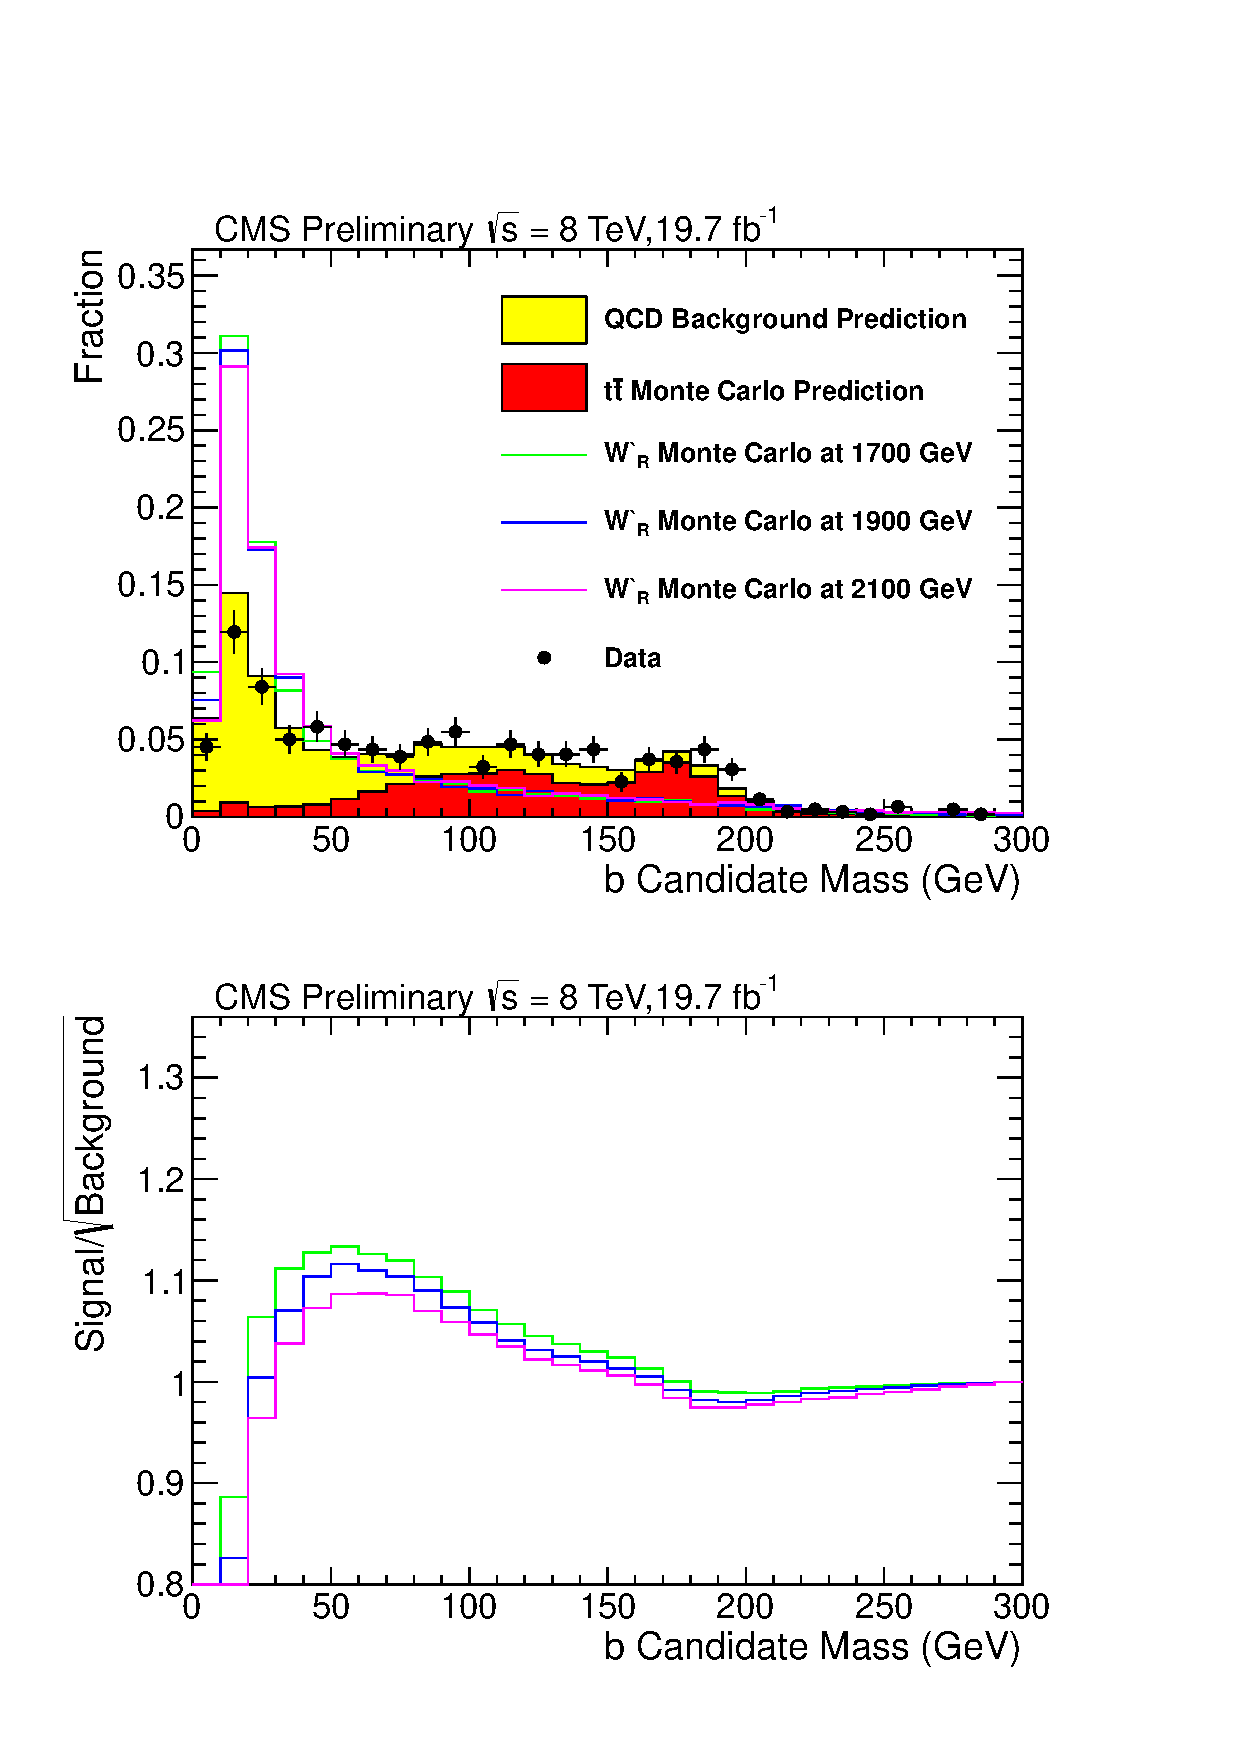
\includegraphics[width=0.7\textwidth]{AN-13-004/figs/bmassdatatosigwithdata.pdf}
\caption{
b candidate mass distributions in data, background, and signal.  Plot of Signal/$\sqrt{\text{Background}}$ (bottom), derived from the top plot. 
This plot includes the full top tagging selection using the background estimation procedure outlined in Chapter \ref{sec:backgroundEstimation}.
}
\label{figs:BmassCOMP}
\end{center}
\end{figure}


\section{Reconstruction of W' Invariant Mass}
\label{sec:fullselection}
The full selection for the reconstruction of the $\wpr$ invariant mass then includes the following offline cuts.
\begin{itemize}
\item One jet with $\pt > 450~\GeV$ identified with the CMS top tagging algorithm as well as subjet b-tagging and N-subjettiness discrimination.
\item One jet with $\pt > 370~\GeV$ with a CSVM b tag and mass$ < 70~\GeV$
\item $|\Delta \phi| > \pi/2$ between the two jets
\item $|\Delta y|$ between the two jets $<$ 1.6 
\end{itemize}
The cutflow for this selection in data, $\ttbar$ Monte Carlo, and right-handed $\wpr$ signal Monte Carlo can be found in Table \ref{table:Cutflow}.
Figure \ref{figs:GCFS} shows this full selection in signal Monte Carlo for various $\wpr$ masses.  



\begin{sidewaystable}
\begin{center}
\begin{small}

\scalebox{0.7}{
\begin{tabular}{c||cccccccccc}
\multicolumn{7}{c}{Number of Selected Events} \\
\hline\hline
\bf{Sample} & \bf{$2 jets$} & \bf{$\pt$} & \bf{$|\Delta y|$} & \bf{$M_{top}$} & \bf{$Nsubjets$} &  \bf{$Minmass$}  & $SJ_{\text{CSVMAX}}$  & $\tau_3/\tau_2$ & $M_{b}$ & \bf{$CSV$}\\
\hline
Data & 13854873$\pm$3722 & 4305244$\pm$2075 & 3376771$\pm$1838 & 992949$\pm$996 & 557489$\pm$747 & 318520$\pm$564 & 50642$\pm$225 & 7200$\pm$85 & 4463$\pm$67 & 277$\pm$17\\
QCD & --- & --- & --- & --- & --- & --- & --- & --- & --- & 248$\pm$4\\
ttbar & 12185$\pm$27.3 & 4718$\pm$17.9 & 4220$\pm$16.9 & 3217$\pm$14.4 & 2742$\pm$13.3 & 2508$\pm$12.6 & 1689$\pm$10.0 & 1024$\pm$7.8 & 178$\pm$3.6 & 37$\pm$1.4\\
M($W`_{R}$) = 1900 & 806$\pm$1.4 & 739$\pm$1.3 & 553$\pm$1.2 & 429$\pm$1.0 & 340$\pm$0.9 & 304$\pm$0.9 & 170$\pm$0.6 & 88$\pm$0.4 & 68$\pm$0.4 & 16$\pm$0.2\\
M($W`_{R}$) = 2100 & 401$\pm$0.7 & 372$\pm$0.7 & 268$\pm$0.6 & 209$\pm$0.5 & 163$\pm$0.4 & 143$\pm$0.4 & 76$\pm$0.3 & 38$\pm$0.2 & 29$\pm$0.2 & 6$\pm$0.1\\
M($W`_{L}$) = 1900 & 796$\pm$2.4 & 703$\pm$2.3 & 531$\pm$2.0 & 414$\pm$1.8 & 312$\pm$1.6 & 274$\pm$1.5 & 138$\pm$1.0 & 58$\pm$0.6 & 44$\pm$0.6 & 10$\pm$0.3\\
M($W`_{L}$) = 2100 & 430$\pm$1.6 & 364$\pm$1.5 & 268$\pm$1.3 & 205$\pm$1.1 & 152$\pm$1.0 & 130$\pm$0.9 & 63$\pm$0.6 & 27$\pm$0.4 & 20$\pm$0.3 & 4$\pm$0.2\\
\end{tabular}
}
\caption{The number of selected events after successive selections as scaled to an integrated luminosity of 19.7~$\fbinv$.  Table reads left to right where the current column implies the previous selection.  The quoted uncertainty is statistical only.  QCD background expectation is only recorded for the full selection, as the average b-tagging rate takes into account the QCD background b fraction increase from b-tagging and subjet b-tagging.  
The first column additionally represents the hemispherical $\delta \phi$ selection between the leading jets.  
The column labeled $\pt$ represents the $\pt$ selection placed on both leading jets.  The signal events are normalized to theory cross-section.}
\label{table:Cutflow}
\end{small}
\end{center}
\end{sidewaystable}




%\begin{sidewaystable}
%\begin{center}
%\begin{small}
%\begin{tabular}{cccccccccc}
%\multicolumn{7}{c}{Data Cutflow} \\
%\hline\hline
%\bf{2 jets} & \bf{$\pt$} & \bf{$|\Delta y|$} & \bf{$M_{top}$} & \bf{$Nsubjets$} &  \bf{$Minmass$} & \bf{$CSV$}  & $\tau_3/\tau_2$ & $M_{b}$ & $SJ_{\text{CSVMAX}}$\\
%\hline
%71.10\% & 22.04\% & 17.28\% & 5.08\% & 2.85\% & 1.63\% & 0.09\% & 0.01\% & 0.007\% & 0.001\%\\
%\end{tabular}
%\caption{Cutflow for Data. Table reads left to right where the current column implies the previous cuts}
%\vspace{1cm}

%\begin{tabular}{cccccccccc}
%\multicolumn{7}{c}{$\ttbar$ Cutflow} \\
%\hline\hline
%\bf{2 jets} & \bf{$\pt$} & \bf{$|\Delta y|$} & \bf{$M_{top}$} & \bf{$Nsubjets$} &  \bf{$Minmass$} & \bf{$CSV$}  & $\tau_3/\tau_2$ & $M_{b}$ & $SJ_{\text{CSVMAX}}$\\
%\bf{2 jets $\pt > 150$} & \bf{Jet1 $\pt > 450$ ; Jet2 $\pt > 370$} & %\bf{$|\Delta y| < 1.6$} & \bf{$140 < M_{top} < 250$} & \bf{$Nsubjets > 2$} &  %\bf{$Minmass > 50$} & \bf{$CSV > 0.679$} & $\tau_3/\tau_2 <0.55$ & $Jet2 Mass < 70$ & $SJ_{\text{CSVMAX}} > 0.679$  \\
%\hline
%26.50\% & 0.91\% & 0.82\% & 0.62\% & 0.52\% & 0.47\% & 0.12\% & 0.06\% & 0.009\% & 0.007\%\\
%\end{tabular}
%\caption{Cutflow for TTbar Monte Carlo. Table reads left to right where the current column implies the previous cuts}
%\vspace{1cm}

%\begin{tabular}{c|cccccccccc}
%\multicolumn{8}{c}{Signal Cutflow} \\
%\hline\hline
%\bf{$M_{\wpr}$} & \bf{2 jets $\pt > 150$} & \bf{Jet1 $\pt > 450$ ; Jet2 $\pt > 370$} & \bf{$|\Delta y| < 1.6$} & \bf{$140 < M_{top} < 250$} & \bf{$Nsubjets > 2$} &  \bf{$Minmass > 50$} & \bf{$CSV > 0.679$} & $\tau_3/\tau_2 <0.55$ & $Jet2 Mass < 70$ & $SJ_{\text{CSVMAX}} > 0.679$ \\
%\bf{$M_{\wpr}$} & \bf{2 jets} & \bf{$\pt$} & \bf{$|\Delta y|$} & \bf{$M_{top}$} & \bf{$Nsubjets$} &  \bf{$Minmass$} & \bf{$CSV$}  & $\tau_3/\tau_2$ & $M_{b}$ & $SJ_{\text{CSVMAX}}$\\
%\hline
%1300 & 77.86\% & 44.33\% & 42.09\% & 27.24\% & 22.55\% & 20.31\% & 7.19\%& 3.79\%& 3.08\%& 2.16\%\\
%1500 & 78.25\% & 52.64\% & 45.20\% & 32.66\% & 26.69\% & 24.15\% & 7.42\%& 3.74\%& 2.95\%& 2.02\%\\
%1700 & 78.01\% & 57.37\% & 45.44\% & 34.47\% & 27.59\% & 24.92\% & 6.67\%& 3.22\%& 2.49\%& 1.68\%\\
%1900 & 77.20\% & 59.36\% & 44.40\% & 34.51\% & 27.19\% & 24.26\% & 5.74\%& 2.72\%& 2.06\%& 1.34\%\\
%2100 & 76.04\% & 59.72\% & 42.95\% & 33.56\% & 26.05\% & 22.70\% & 4.87\%& 2.20\%& 1.63\%& 1.02\%\\
%2300 & 74.20\% & 58.37\% & 40.87\% & 31.80\% & 24.63\% & 20.70\% & 4.14\%& 1.87\%& 1.37\%& 0.84\%\\
%2700 & 69.36\% & 51.81\% & 35.51\% & 27.13\% & 21.51\% & 16.32\% & 3.06\%& 1.34\%& 0.99\%& 0.61\%\\
%3100 & 63.12\% & 40.89\% & 28.57\% & 21.23\% & 17.34\% & 12.28\% & 2.54\%& 1.15\%& 0.86\%& 0.55\%\\
%\end{tabular}
%\caption{Cutflow for Right-Handed $\wpr$ signal Monte Carlo. Table reads left to right where the current column implies the previous cuts}
%\label{table:Cutflows}
%\end{small}
%\end{center}
%\end{sidewaystable}

\begin{figure}[htcb]
\begin{center}
\subfigure{\label{figs:GCFSright}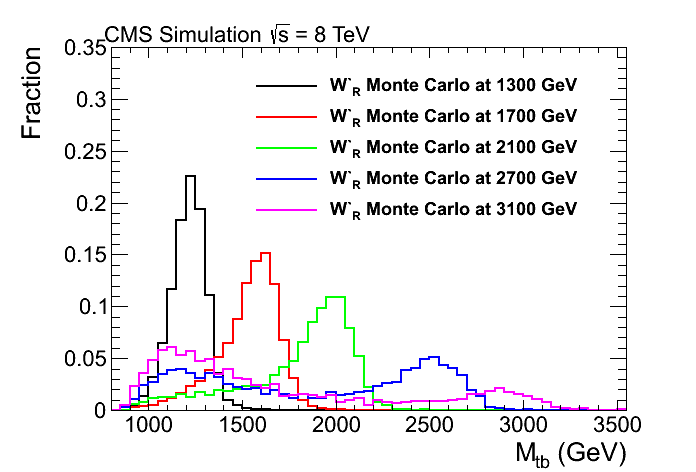
\includegraphics[width=0.45\textwidth]{AN-13-004/figs/SignalMCFScomparison}}\\
\subfigure{\label{figs:GCFSleft}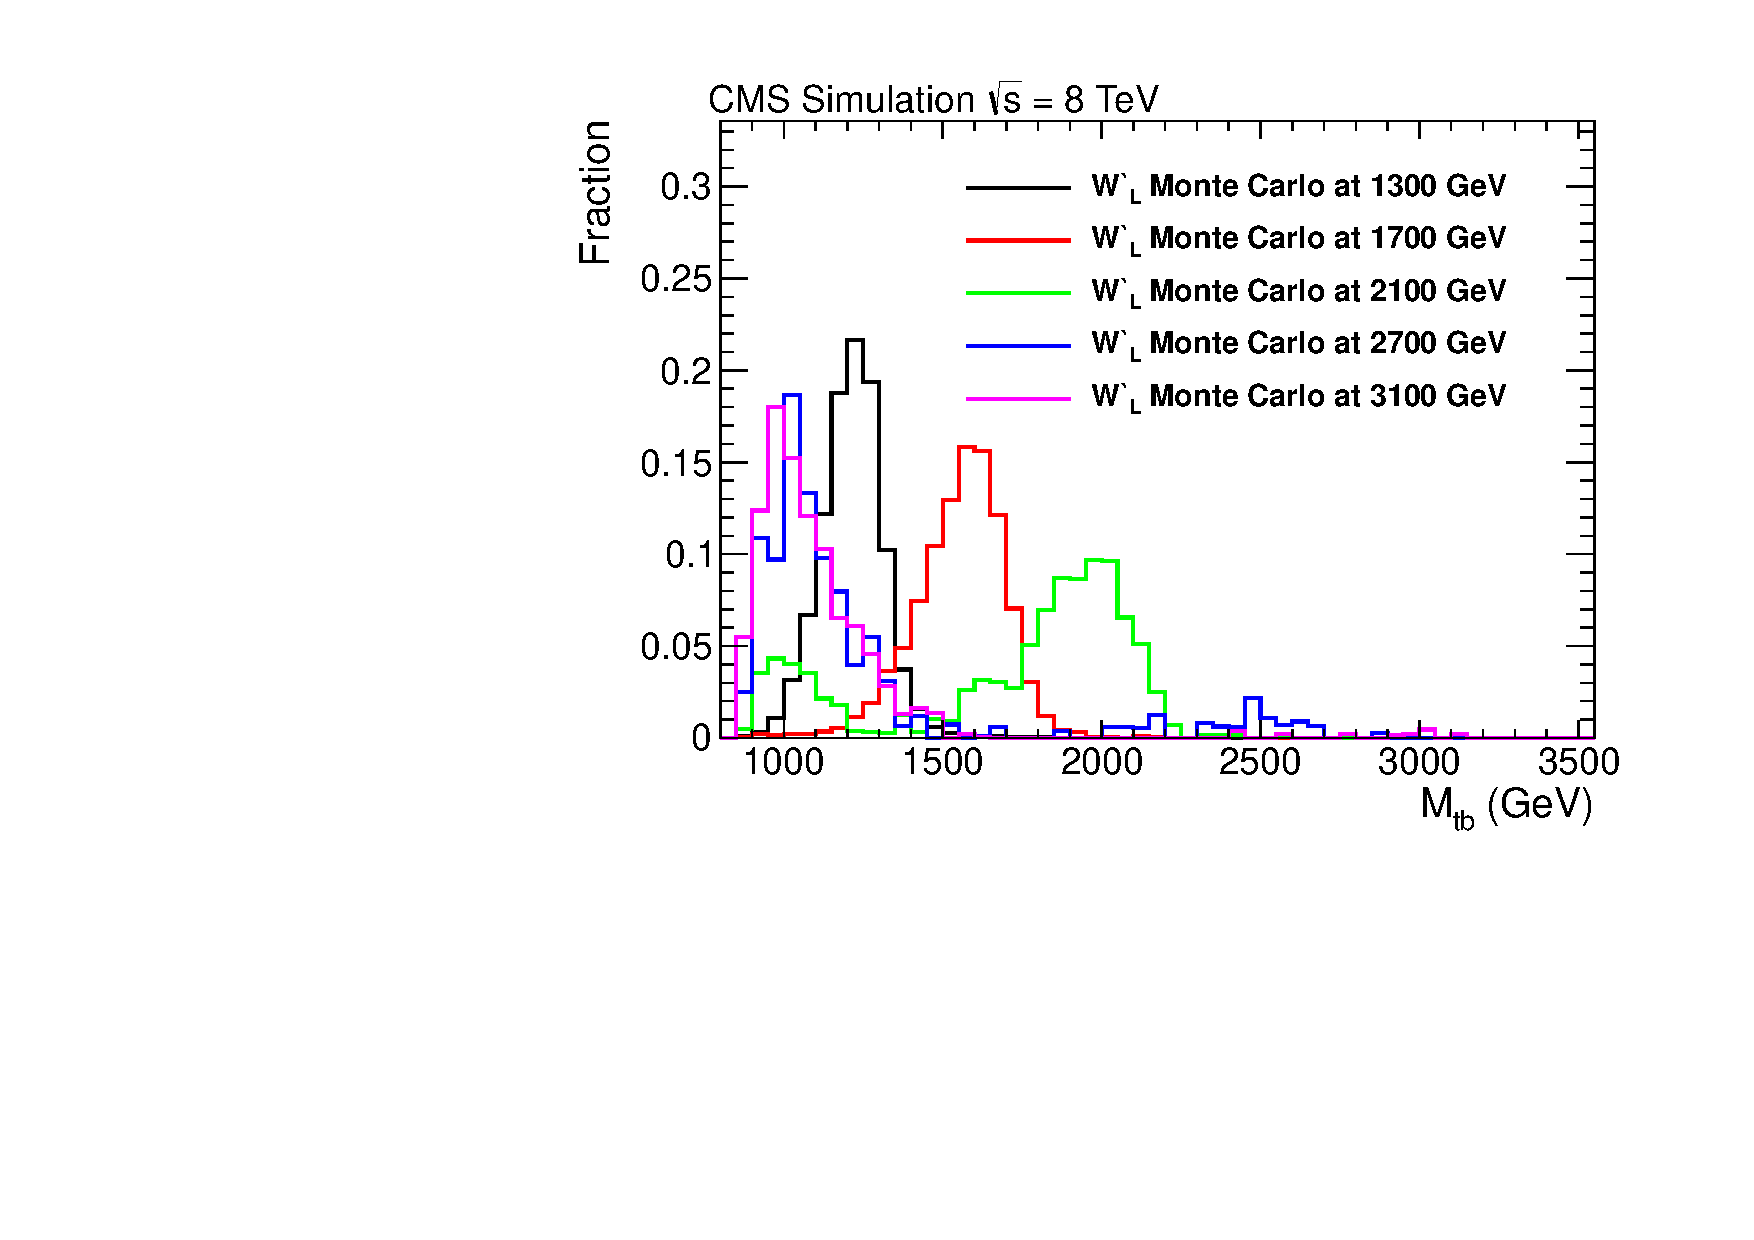
\includegraphics[width=0.45\textwidth]{AN-13-004/figs/SignalLeftMCFScomparison.pdf}}
\subfigure{\label{figs:GCFSmixed}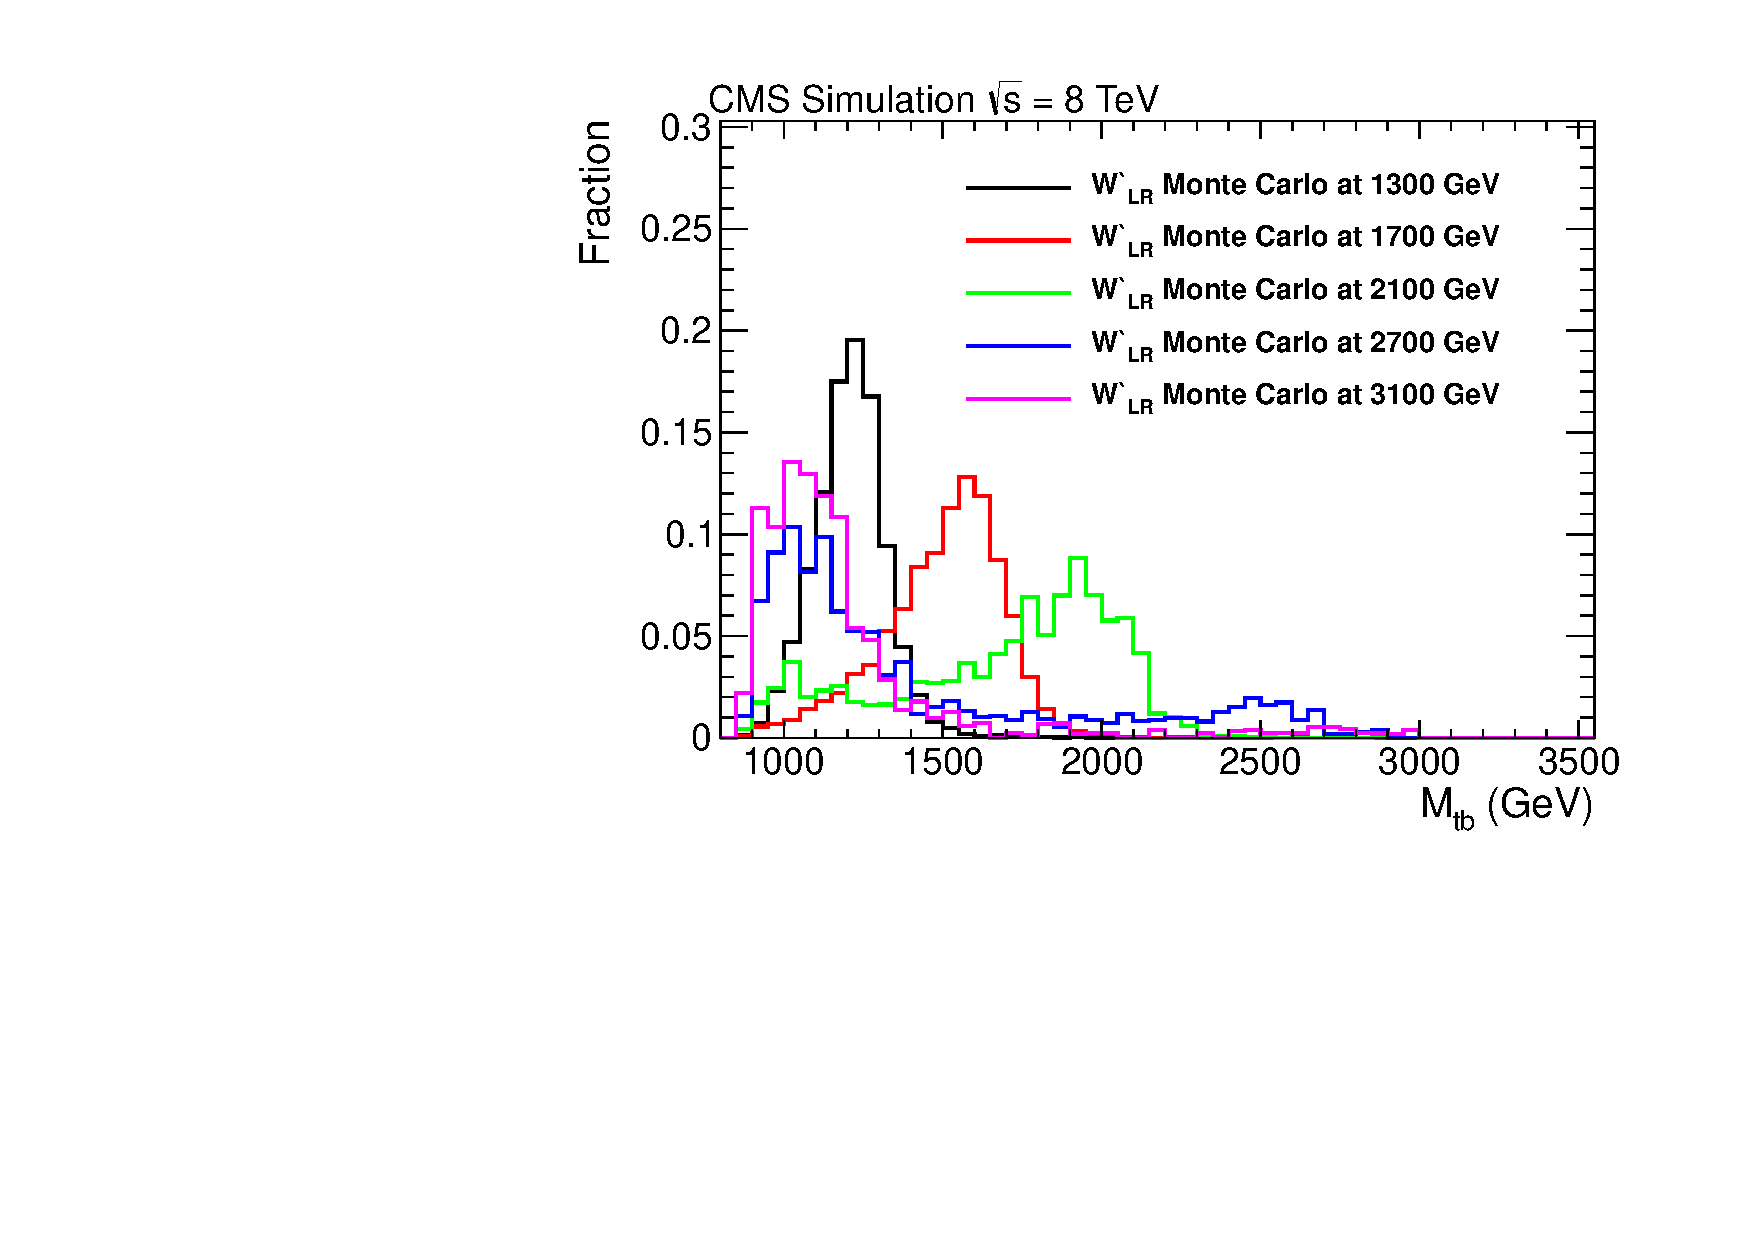
\includegraphics[width=0.45\textwidth]{AN-13-004/figs/SignalMixedMCFScomparison.pdf}}
\caption{
Full selection applied to $W`_{R}$ (top) $W`_{L}$ (bottom-left) and $W`_{LR}$ (bottom-right).  The bimodal structure seen in the $M_{tb}$ spectrum for high $\wpr$ mass is a feature common to high-mass large-width resonances and represents the superposition of a $\wpr$ resonance and a rapidly falling parton distribution function. 
}
\label{figs:GCFS}
\end{center}
\end{figure}

%\begin{figure}[htcb]
%\centering
%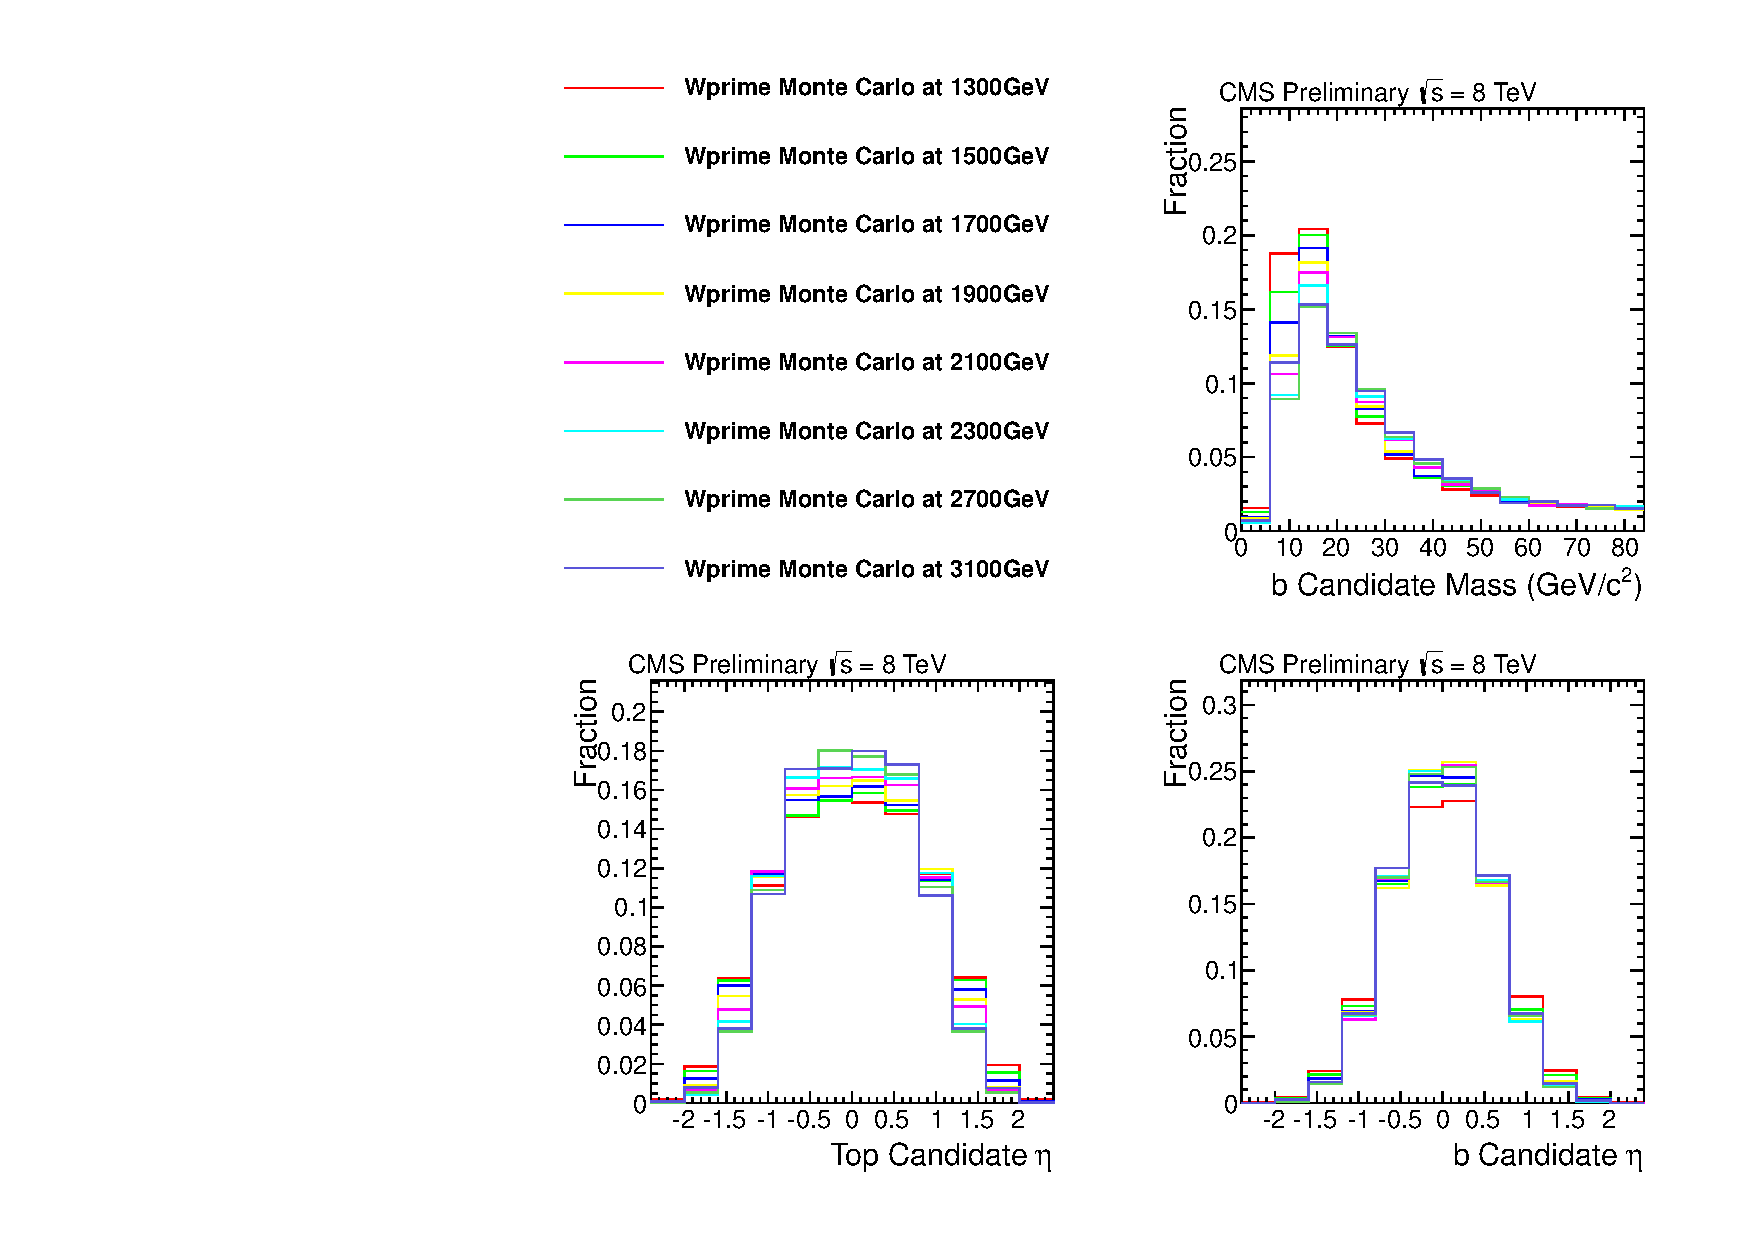
\includegraphics[width=0.9\textwidth]{AN-13-004/figs/KinPlots_Signal1}
%\caption{Full selection in right-handed $\wpr$ signal Monte Carlo kinematic distributions}
%\label{figs:kinplotssignal1}
%\end{figure}

%\begin{figure}[htcb]
%\centering
%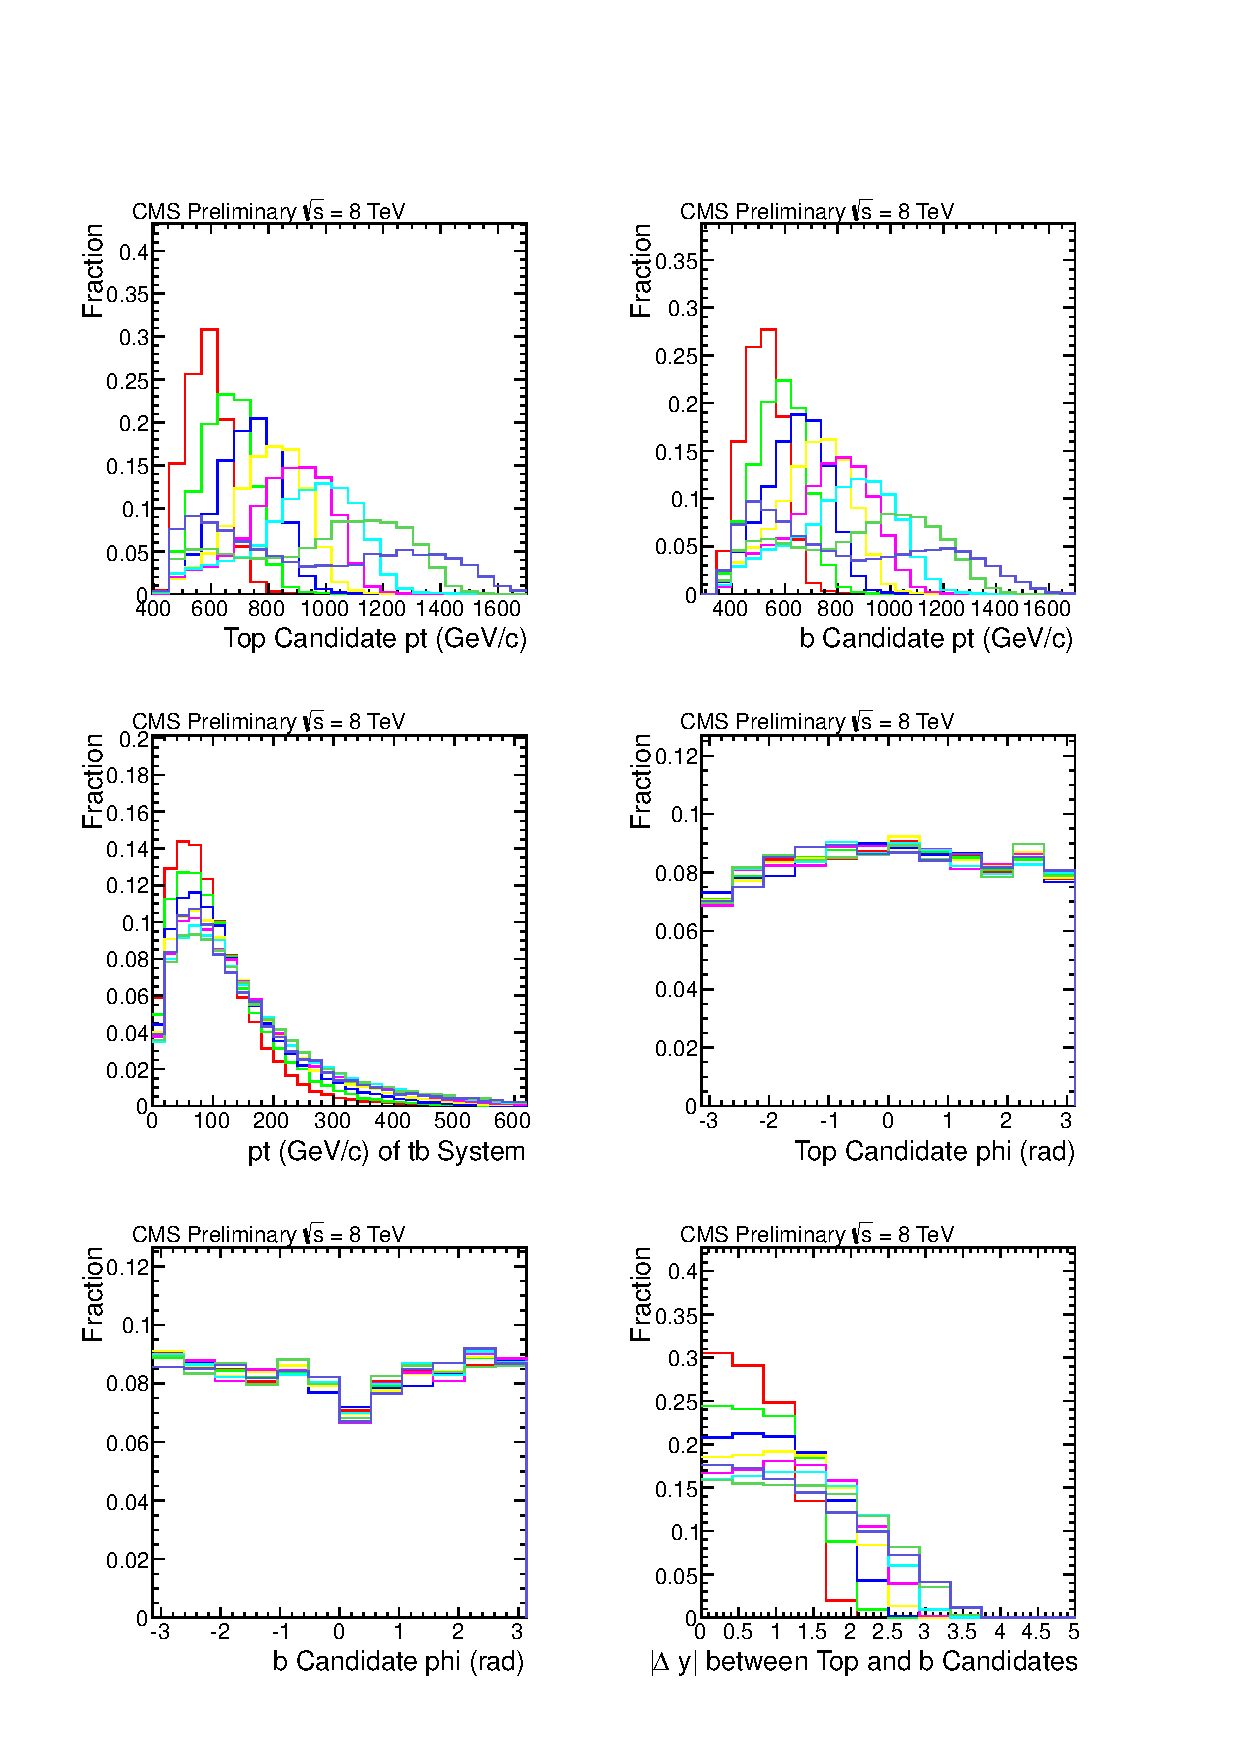
\includegraphics[width=0.9\textwidth]{AN-13-004/figs/KinPlots_Signal2}
%\caption{Full selection in right-handed $\wpr$ signal Monte Carlo kinematic distributions}
%\label{figs:kinplotssignal2}
%\end{figure}
\clearpage

\clearpage
\newpage
\chapter{Background Estimation}
\label{sec:backgroundEstimation}
An essential part of the analysis is the data driven estimation of the QCD background.  
The background estimate relies on extracting the average b-tagging rate of a QCD jet in our signal region.  
We extract this rate by making use of the following sideband.
\section{Substructure Sideband}
\label{sec:sideband}
We define the substructure sideband as events passing all signal region cuts but explicitly 
failing the top jet substructure cut on the number of subjets.  Additionally, to ensure similar parton flavor distributions in the signal region and sideband (Figure \ref{figs:partonflav}), 
we also include subjet CSV discrimination. The top jet sideband is defined as:
\begin{eqnarray}
	140  <  m_{\text{jet}}  <  250 \GeV \\
	N_{\text{subjets}}  \leq  2 \\
	SJ_{\text{CSVMAX}} \geq 0.679 
\end{eqnarray}
The Minimum Pairwise Mass variable described in Section \ref{sec:toptagging} is not defined in this choice of sideband.

\section{QCD Background Estimation}
\label{sec:qcdBackgroundEstimationProcedure}
\label{sec:tagrateparameterization}
The estimation of QCD background is performed by extracting the probability to tag a b jet in the sideband. 
The primary assumption used in background estimation is that the average b-tagging probability 
for QCD multijets in the signal region is nearly identical to the sideband. Figure \ref{figs:partonflav}  shows the parton flavor distribution for signal region and sideband in QCD MC, the
 nearly identical composition can be considered motivation for the previous assumption.

To extract a QCD background estimate, we weight the events that pass the full selection in the signal region before the b-tagging requirement is applied by 
the average b-tagging probability (measured in the top jet sideband).  This gives us an accurate expectation of the QCD background in the signal region.
The b-tagging rate is defined as the inverse ratio of the number of b candidate jets, 
defined as $\pt > 370~\GeV$ jets in the hemisphere opposite the top jet to the number of b candidate jets that are b-tagged.  
%This ratio is shown if Figure \ref{figs:partonflav} in bins of parton flavor for signal region and sideband as extracted from QCD Monte Carlo.    

\begin{figure}[htbp]
\begin{center}
\subfigure{\label{figs:partonflavCOMP}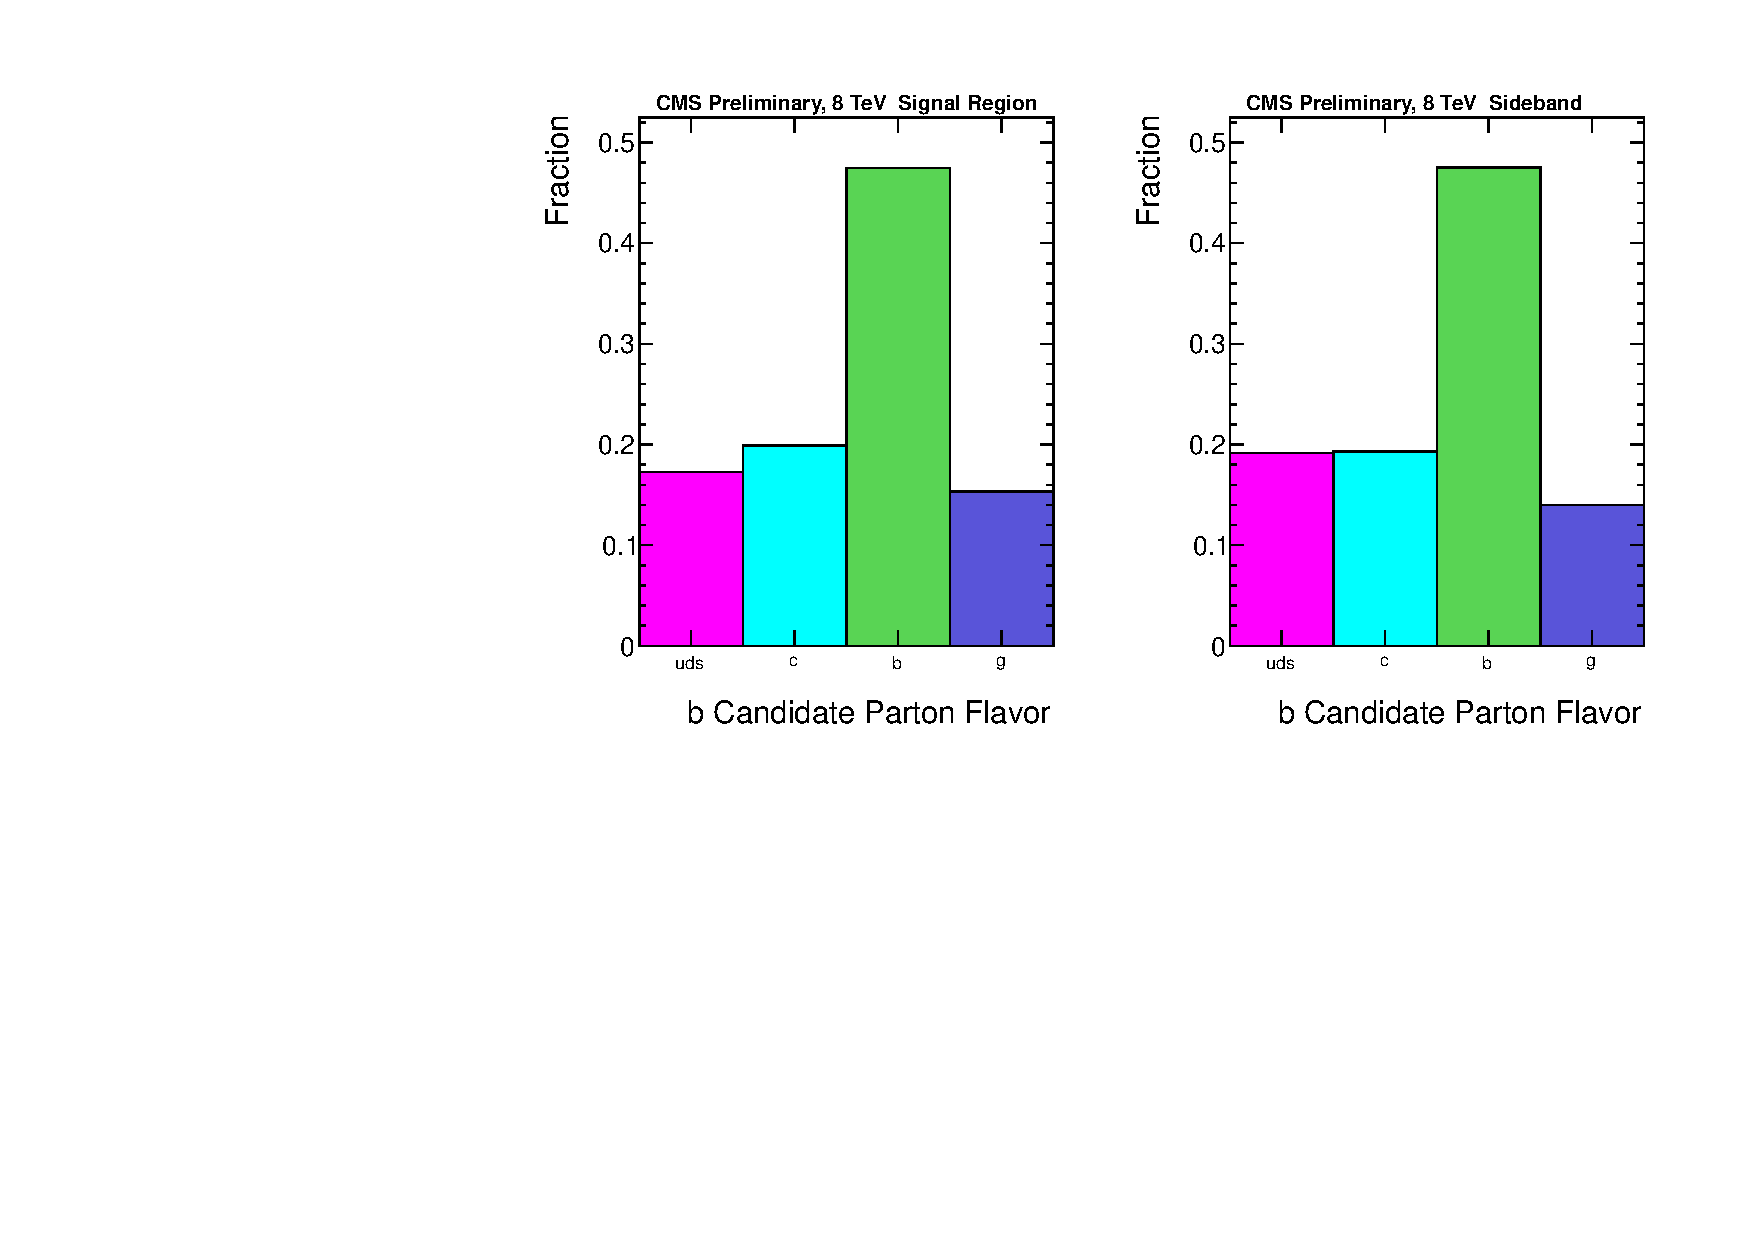
\includegraphics[width=1.0\textwidth]{AN-13-004/figs/partonflavCOMP}}\\ 
\caption{
Comparison of jet parton flavor composition from the signal region and sideband.
%(b) Comparison of average b-tagging rate as a function of jet parton flavor from the signal region and sideband.  
}
\label{figs:partonflav}
\end{center}
\end{figure}

The parameterization of the average b-tagging rate is two dimensional and considers both the $|\eta|$ and $\pt$ of the b candidate jets.  
We break down data into three distinct regions in $|\eta|$. 


\begin{itemize}
	\item \text{Low } $(0.0 < |\eta| \leq 0.5)$
	\item \text{Transition } $(0.5 < |\eta| \leq 1.15)$ 
	\item \text{High } $(1.15 < |\eta| \leq 2.4)$ 
\end{itemize}

The regions in $|\eta|$ are then individually parameterized in $\pt$ to produce the average b-tagging rate.  We perform this parameterization 
of the b-tagging rate in an attempt to constrain the kinematic correlations inherent in b-tagging.

To smooth out the binning of the average b-tagging rate, a study of functional fits was conducted for the average b-tagging rate (see Figure \ref{figs:BKGFITCOMP}).
We chose the bifurcated polynomial fit based on observed representation of the data.  The fitting function is as follows

\begin{eqnarray}
f(x) =
\begin{cases}
p_0+p_1x+p_2(x-\text{a})^2, & \text{if x} < \text{a} \\
p_0+p_1x+p_3(x-\text{a})^2, & \text{if x}\geq\text{a}
\end{cases}
\end{eqnarray}

Here, the parameters $p_0$ through $p_3$ are inputs to the fitting algorithm, and x is the $\pt$ of the b candidate jet.  The parameter a is the bifurcation point, and is chosen manually for each region in $\eta$.
It is chosen to be 500$~\GeV$, 500$~\GeV$, and 550$~\GeV$ for the low, transition, and high $\eta$ regions respectively.
This piecewise function allows for two characteristic ranges to fit a polynomial, which makes a good fit for the different functional forms of the average b-tagging rate regions that we use.

The errors on the average b-tagging rate are then extracted using the full covariance matrix as obtained from output of the fitting 
algorithm.   
Additionally, we assign a systematic uncertainty to cover the choice of the fit function (see Chapter \ref{sec:systematics}) based on several alternative functional forms.
Figure \ref{figs:tagsandprobes8TeV} shows the tags (numerator) and probes (denominator) of the tagging rate.
Figure \ref{figs:tagrateetafit} shows the three fitted average b-tagging rates parameterized in $\pt$.  

%\section{Treatment of QCD Background Events with Double Top Tags}
%\label{sec:dubtags}
%As mentioned in Section \ref{sec:analysisStrategy}, the analysis uses  hemispherically separated dijets as top and b candidates.  
%Because it is not obvious which candidate will be the leading jet, both are considered.  If the event registers a count in either of these configurations, the other is not considered to prevent double counting.  
%However, the QCD background estimate is based on the probability of recording a count and thus the cut to prevent double counting should not be applied when filling the QCD background.  
%This type of event occurs when both the leading and sub leading jet are top tagged, and both jets are considered for b-tagging.  
%Note that this does not impact the treatment of ttbar, and these events are simply of rare QCD origin (see Section \ref{sec:ttSubtraction}). 
%An event that records two counts in the background estimation has the physical meaning that the event has two chances to tag a b jet.

\section{$\ttbar$ Subtraction}
\label{sec:ttSubtraction}
\label{sec:bsttSubtraction}
The $\ttbar$ contribution to background is computed from Monte Carlo that passes the full selection. To avoid double-counting, we must remove $\ttbar$ from our QCD estimate. 
In creating the b-tagging rate, the $\ttbar$ contribution to the numerator and denominator is subtracted away using $\ttbar$ Monte Carlo. 
Additionally, we account for the $\ttbar$ contamination of the QCD background estimate by applying 
the average b-tagging rate to $\ttbar$ Monte Carlo in the same way as data.  This is a measure of $\ttbar$ that is expected to fall 
through the QCD background estimate and is subtracted away. 

%We can similarly consider the possible effect of the single-top contribution to this tag rate. 
%However, due to the very low background from single-top, we find that we do not need to modify the average b-tagging rate. 
%Table \ref{table:singletop} shows a comparison of the various contribution to the average b-tagging rate.  
%Theoretically, the signal could also be present in the 
%pre tagged and post tagged sample, which could bias the background estimation.  However, in practice it is seen that this effect is a fraction of a 
%percent and is thus much smaller than the uncertainty placed on the background estimation.

\begin{table}
\begin{center}
\begin{tabular}{|c||c|c|c|} 
\hline
  & $\eta_1$ & $\eta_2$ & $\eta_3$ \\
\hline
\hline
pretag QCD & 15922 ($99.77\%$) & 14396 ($99.79\%$) & 5494 ($99.81\%$)\\
tagged QCD & 924 ($99.17\%$) & 847 ($99.16\%$) & 285 ($99.54\%$)\\
pretag $\ttbar$ & 37 ($0.23\%$) & 31 ($0.21\%$) & 11 ($0.19\%$)\\
tagged $\ttbar$ & 8 ($0.83\%$) & 7 ($0.84\%$) & 1 ($0.46\%$)\\
pretag signal at 1300$\GeV$ & 108 ($0.67\%$) & 77 ($0.53\%$) & 17 ($0.30\%$)\\
tagged signal at 1300$\GeV$ & 37 ($3.94\%$) & 24 ($2.87\%$) & 4 ($1.44\%$)\\
pretag signal at 1500$\GeV$ & 62 ($0.39\%$) & 39 ($0.27\%$) & 8 ($0.14\%$)\\
tagged signal at 1500$\GeV$ & 17 ($1.86\%$) & 11 ($1.28\%$) & 2 ($0.67\%$)\\
pretag signal at 1700$\GeV$ & 31 ($0.19\%$) & 19 ($0.13\%$) & 3 ($0.06\%$)\\
tagged signal at 1700$\GeV$ & 8 ($0.82\%$) & 4 ($0.53\%$) & 1 ($0.25\%$)\\
pretag signal at 1900$\GeV$ & 15 ($0.09\%$) & 9 ($0.06\%$) & 1 ($0.02\%$)\\
tagged signal at 1900$\GeV$ & 3 ($0.31\%$) & 2 ($0.20\%$) & 0 ($0.07\%$)\\
pretag signal at 2100$\GeV$ & 7 ($0.04\%$) & 4 ($0.03\%$) & 0 ($0.01\%$)\\
tagged signal at 2100$\GeV$ & 1 ($0.13\%$) & 1 ($0.09\%$) & 0 ($0.03\%$)\\
\hline
\end{tabular}
\end{center}
\caption{Number of tagged and pretagged events for each background sample and percent contribution to overall average b-tagging rates.  Additionally, signal samples are investigated.  
The percents indicated are out of the total QCD + $\ttbar$ expectation and the signal samples are scaled to theory cross-section.}
\label{table:singletop}
\end{table}

\begin{figure}[htcb]
\centering
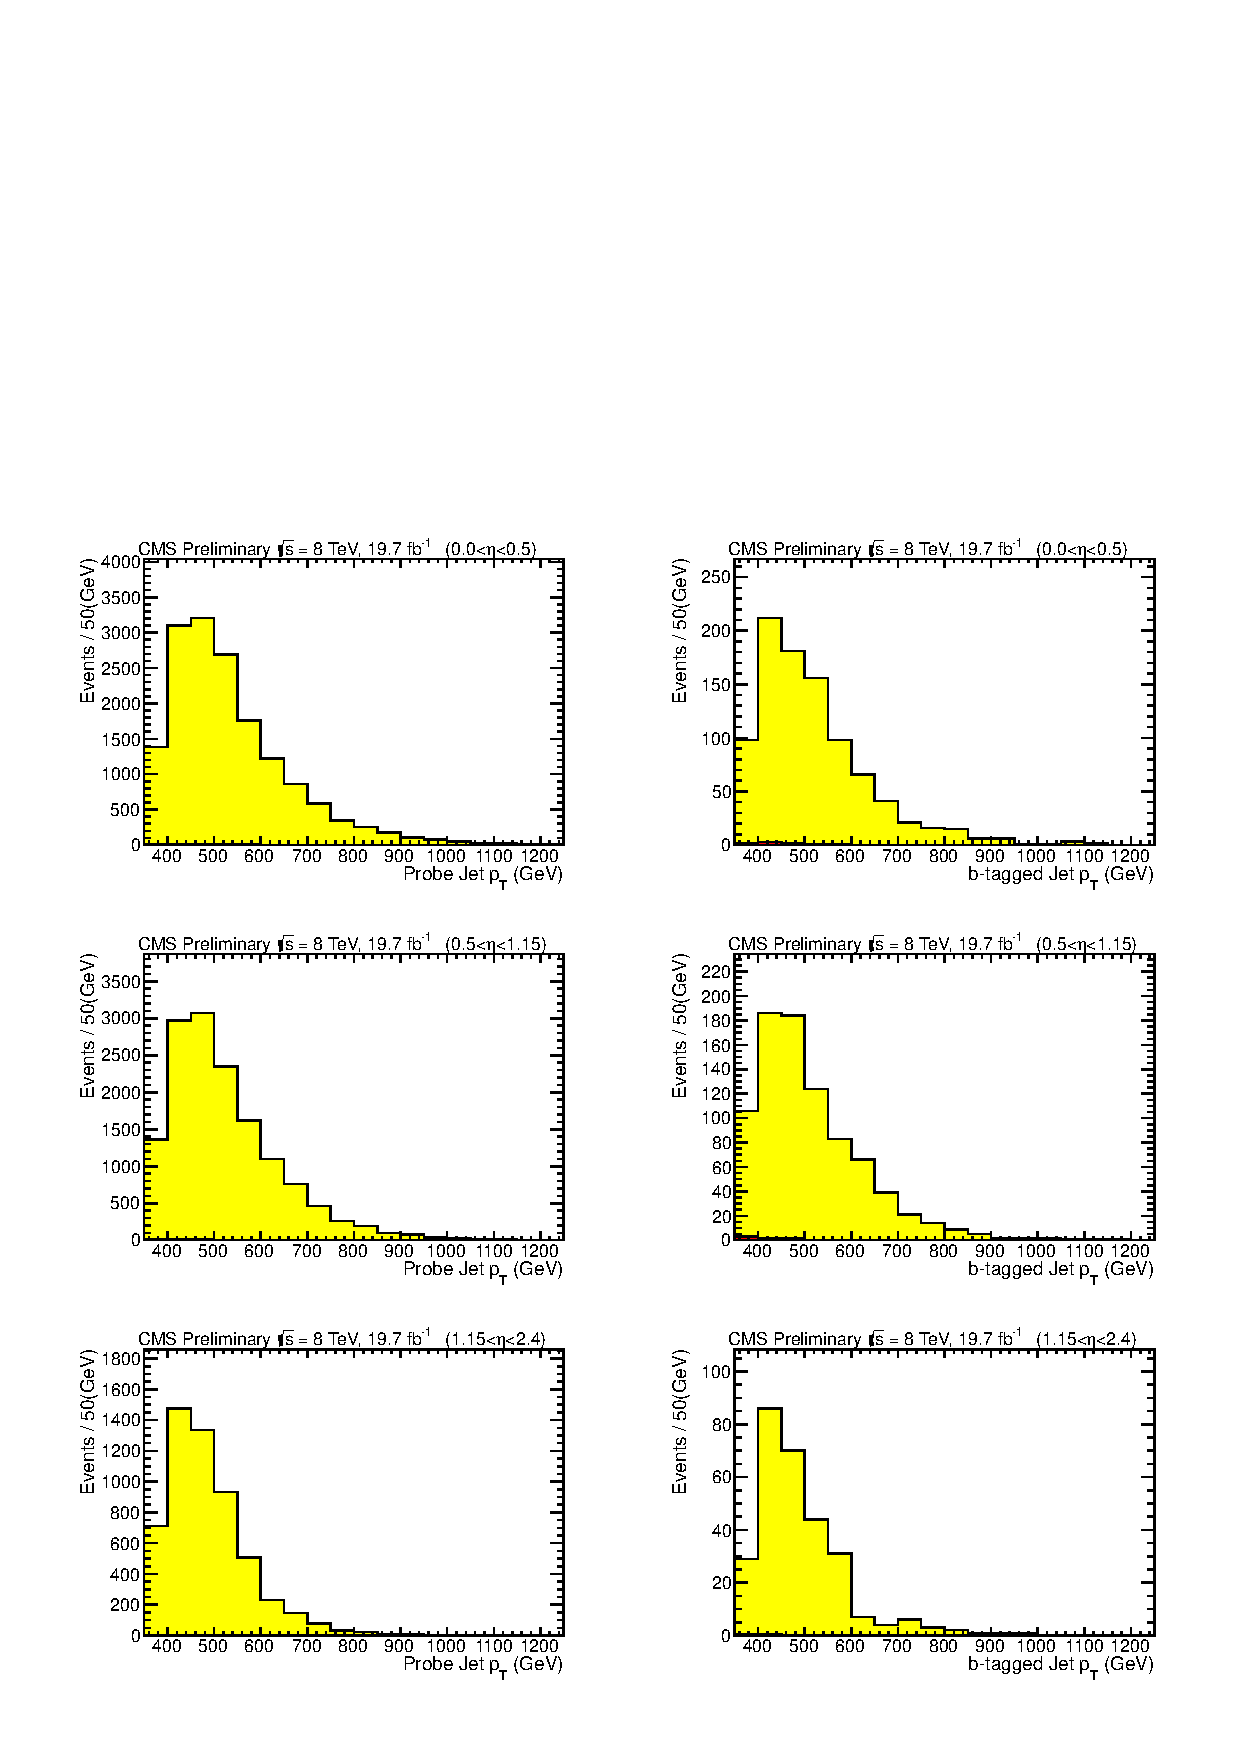
\includegraphics[width=1.0\textwidth]{AN-13-004/figs/tagsandprobes}
\caption{The tags and probes used for the average b-tagging rate in each of the three regions in $|\eta|$ .  Here, tags are the numerator and probes are the denominator of the average b-tagging rate}
\label{figs:tagsandprobes8TeV}
\end{figure}

\begin{figure}[htcb]
\begin{center}
\subfigure{\label{figs:tagrateeta1fit}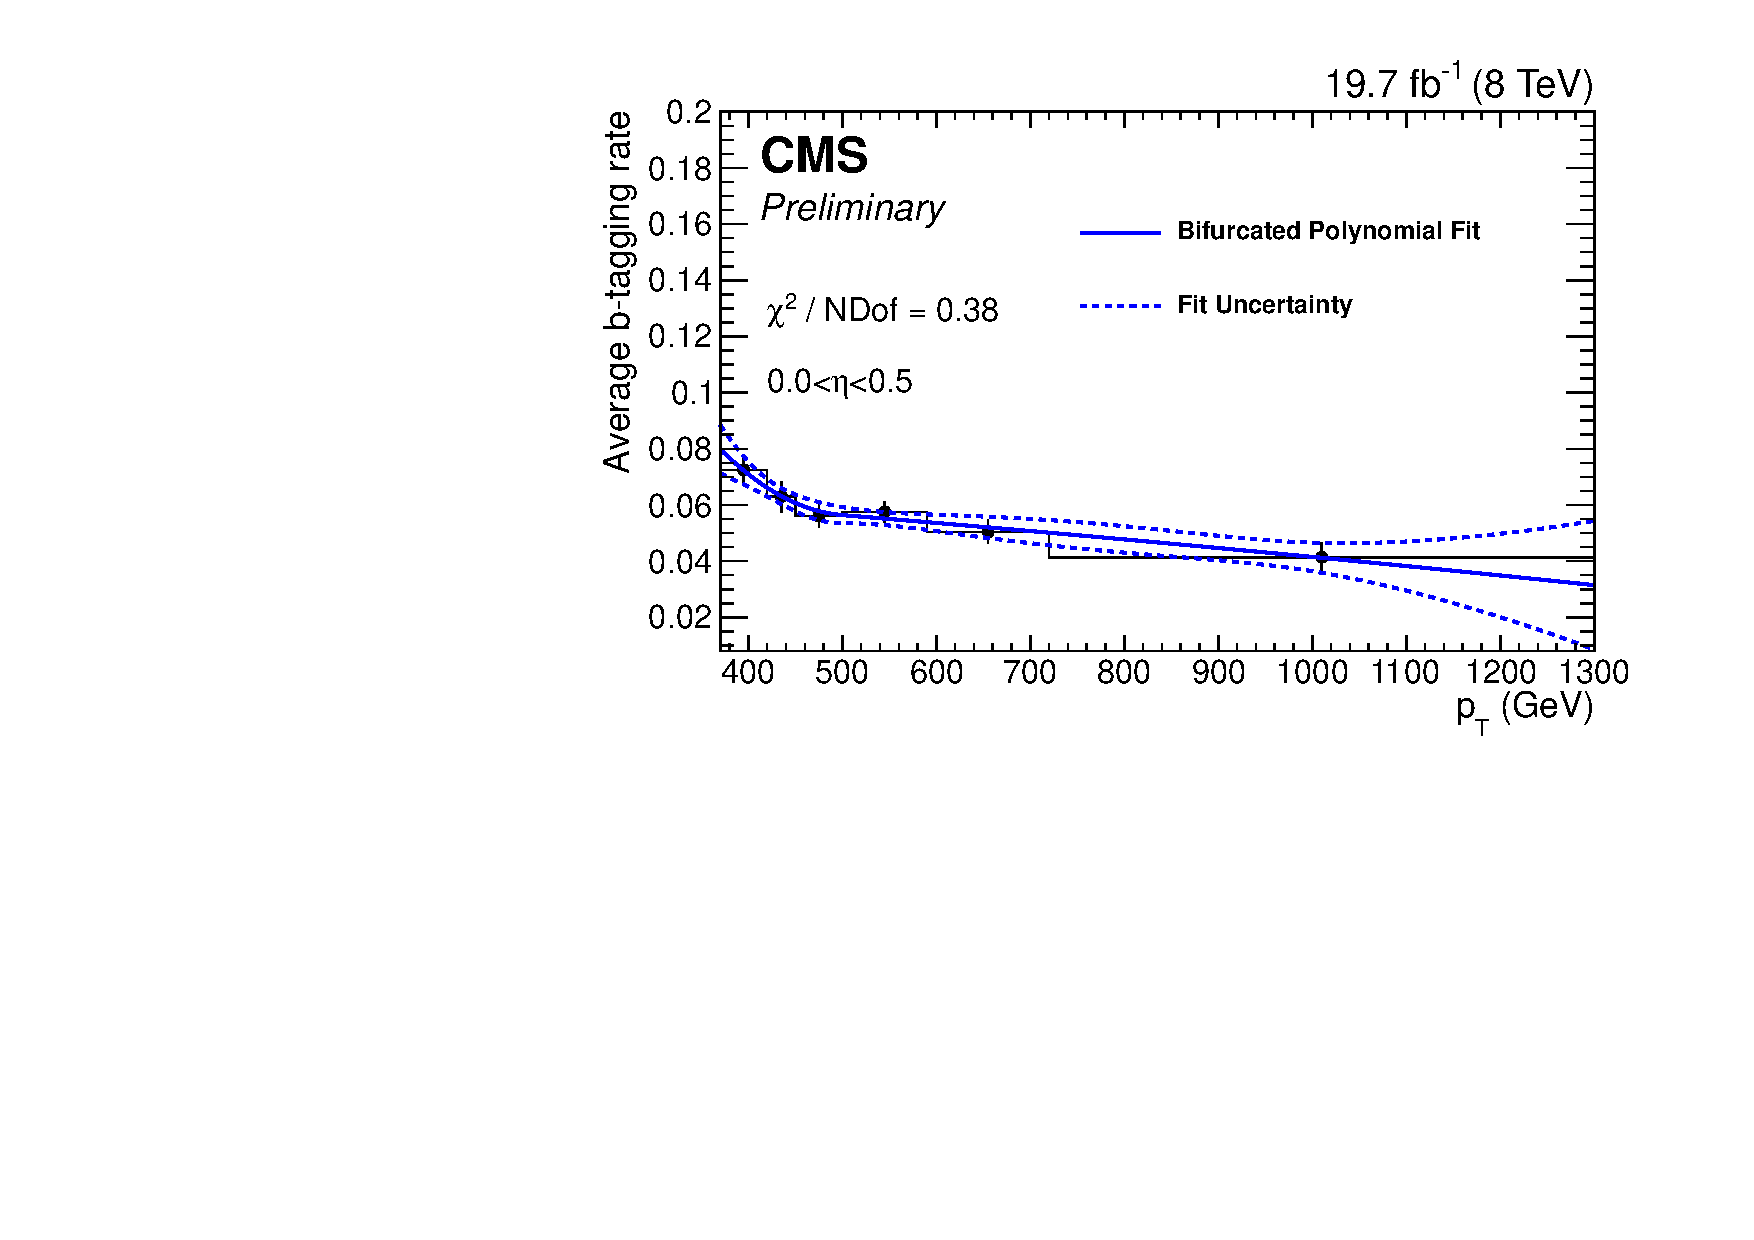
\includegraphics[width=0.7\textwidth]{AN-13-004/figs/tagrateeta1fitBP.pdf}}\\
\subfigure{\label{figs:tagrateeta2fit}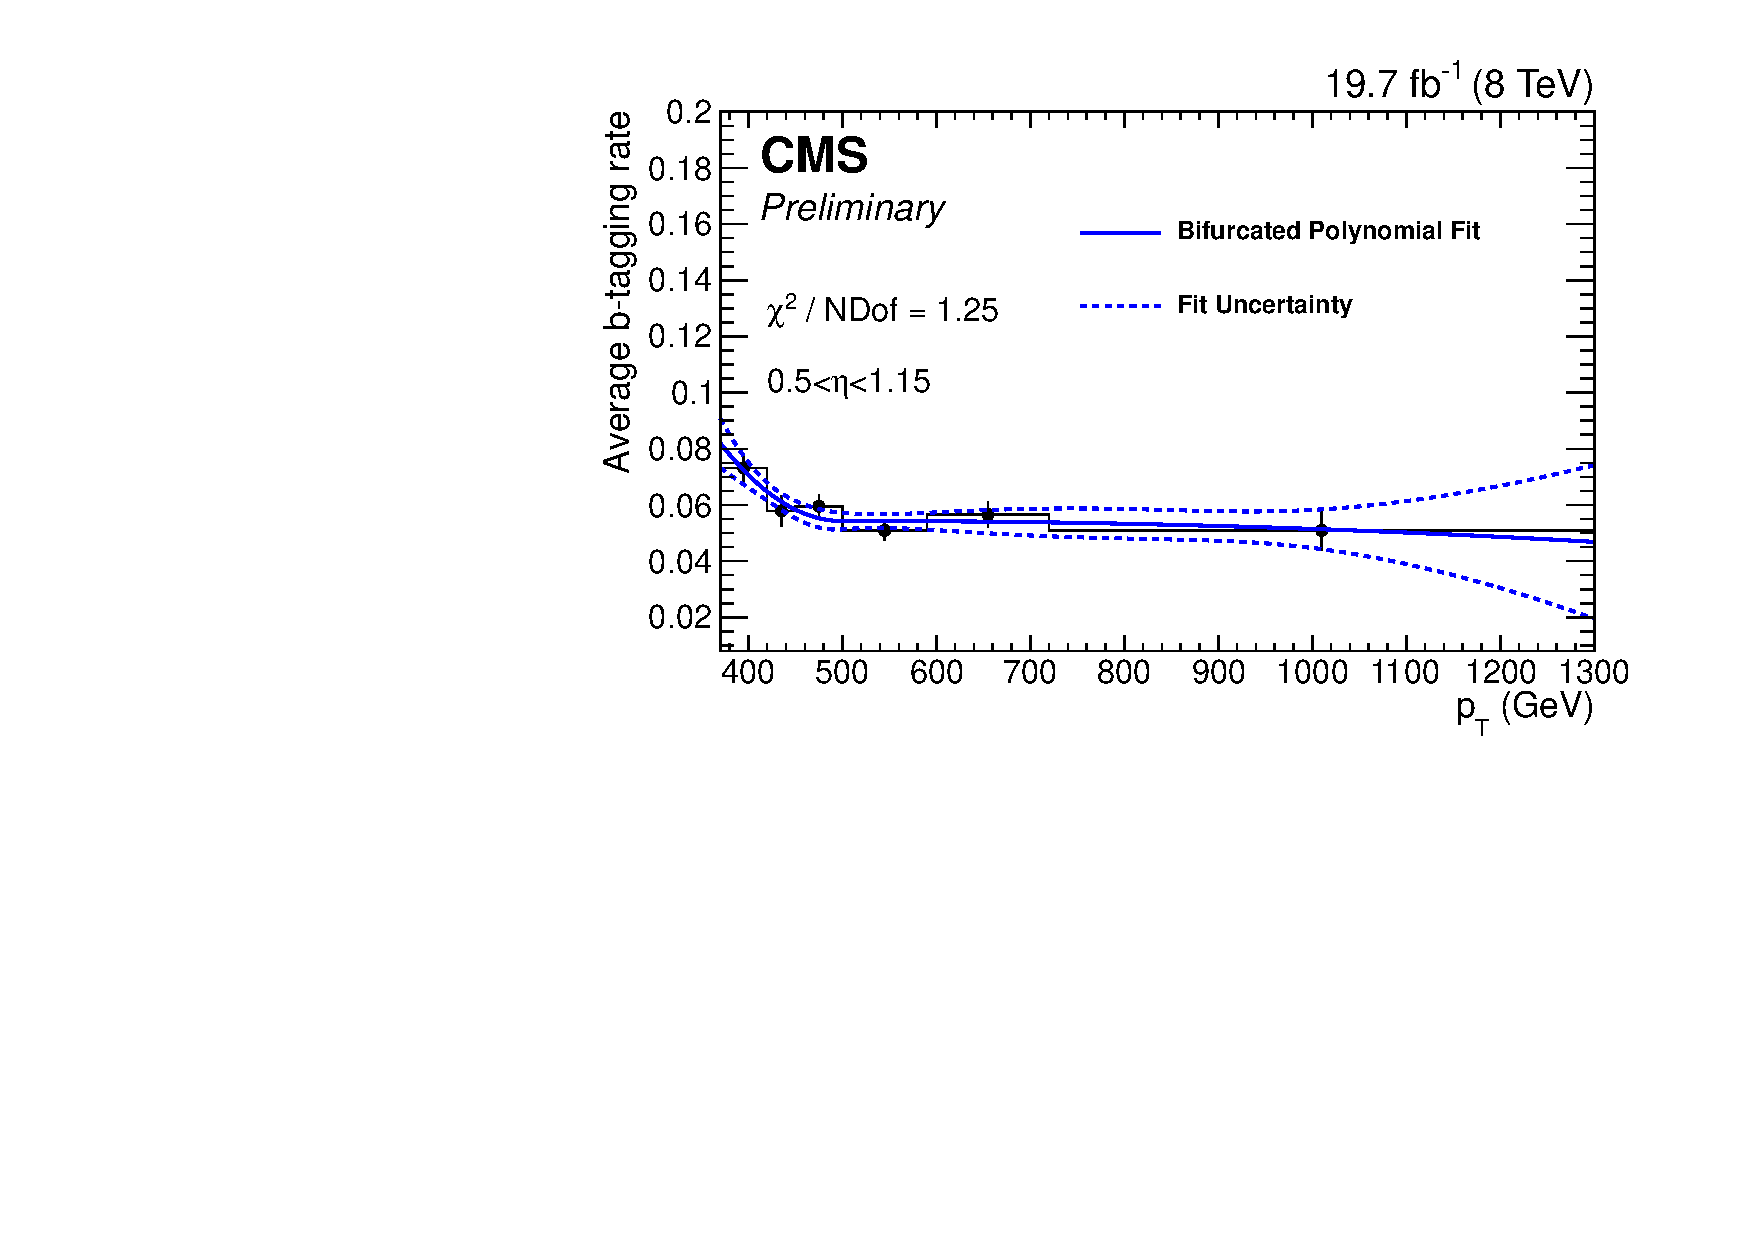
\includegraphics[width=0.7\textwidth]{AN-13-004/figs/tagrateeta2fitBP.pdf}}\\
\subfigure{\label{figs:tagrateeta3fit}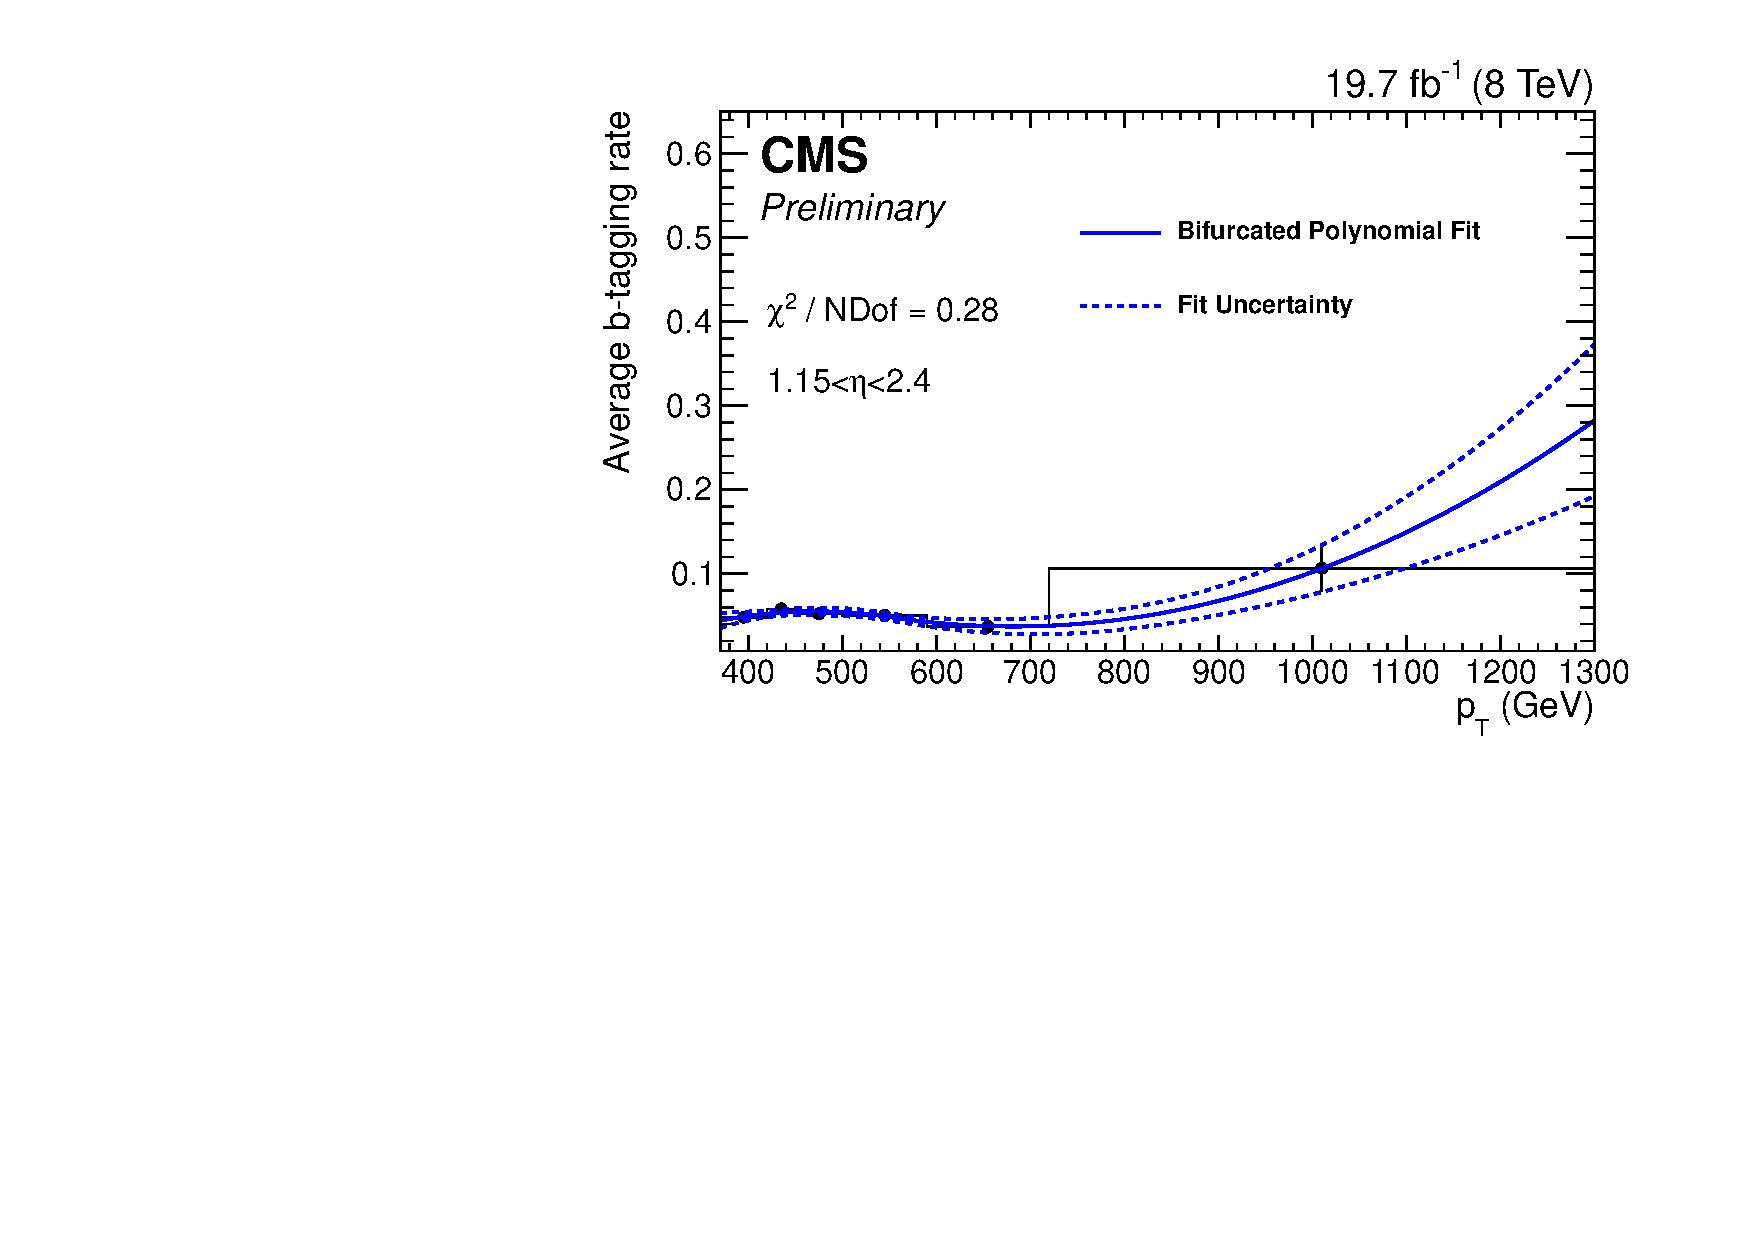
\includegraphics[width=0.7\textwidth]{AN-13-004/figs/tagrateeta3fitBP.pdf}}
\caption{
$\pt$ parameterized average b-tagging rate from
(a) Low $\eta$ region  
(b) Transition $\eta$ region 
(c) High $\eta$ region. 
  The average b-tagging rate is shown in black, the polynomial fit is shown in blue, and the propagated errors from the fit are shown as a blue dashed line.}
\label{figs:tagrateetafit}
\end{center}
\end{figure}

%\section{QCD Closure}
%As a closure test, the background estimation is performed on the QCD Monte Carlo samples listed in Table \ref{table:datasetsQCD}.  

%\begin{table}
%\begin{center}
%\begin{tabular}{|p{0.7\linewidth}|r|} 
%\hline
%\bf{Sample} & \bf{Cross-Section} \\
%\hline
%/QCD\_Pt-300to470\_TuneZ2star\_8TeV\_pythia6/Summer12-PU\_S7\_START52\_V9-v1/AODSIM & 1759.6 \\
%/QCD\_Pt-470to600\_TuneZ2star\_8TeV\_pythia6/Summer12-PU\_S7\_START52\_V9-v1/AODSIM & 113.9 \\
%/QCD\_Pt-600to800\_TuneZ2star\_8TeV\_pythia6/Summer12-PU\_S7\_START52\_V9-v1/AODSIM & 27.0 \\
%/QCD\_Pt-800to1000\_TuneZ2star\_8TeV\_pythia6/Summer12-PU\_S7\_START52\_V9-v1/AODSIM & 3.57 \\
%/QCD\_Pt-1000to1400\_TuneZ2star\_8TeV\_pythia6/Summer12-PU\_S7\_START52\_V9-v1/AODSIM & 0.738 \\
%/QCD\_Pt-1400to1800\_TuneZ2star\_8TeV\_pythia6/Summer12-PU\_S7\_START52\_V9-v1/AODSIM & 0.0335 \\
%\hline
%\end{tabular}
%\end{center}
%\caption{QCD Monte Carlo Sample.}
%\label{table:datasetsQCD}
%\end{table}

%The extracted tagrates are shown in Figure\ref{figs:tagrateetafitQCD}.  
%Here, the tagrate was extracted with the procedure noted in Sections \ref{sec:qcdBackgroundEstimationProcedure} 
%and \ref{sec:tagrateparameterization}, as the $\ttbar$ contribution is not present here.  The closure test was performed by using the tagrates to weigh 
%pre b tagged jets within the relevant $|\eta|$ and $\pt$ regions with the tagrate as fitted with the bifurcated polynomial fit outlined in Section \ref{sec:tagrateparameterization}.  For this closure test, 
%the tagrates were extracted from the sideband using only even numbered events from the Monte Carlo and applied to only the odd numbered events in the signal region.  
%The results are shown in Figure\ref{figs:QCDClosure}.    
%The Monte Carlo here is scaled to the total number of events in our full selection in data, and the error bars represent 
%$\sqrt{N}$ where N is the bin content.  This procedure allows us to investigate the effect of any possible bias given the current integrated luminosity.  The QCD closure analysis performed on the full statistic QCD sample can be seen in 
%\ref{figs:QCDClosure1}.  
%The tagrate comparison of signal region and sideband is shown in Figure\ref{figs:tagrateetaQCD_withSR}

%\begin{figure}[htcb]
%\begin{center}
%\subfigure{\label{figs:tagrateeta1fitBPQCD}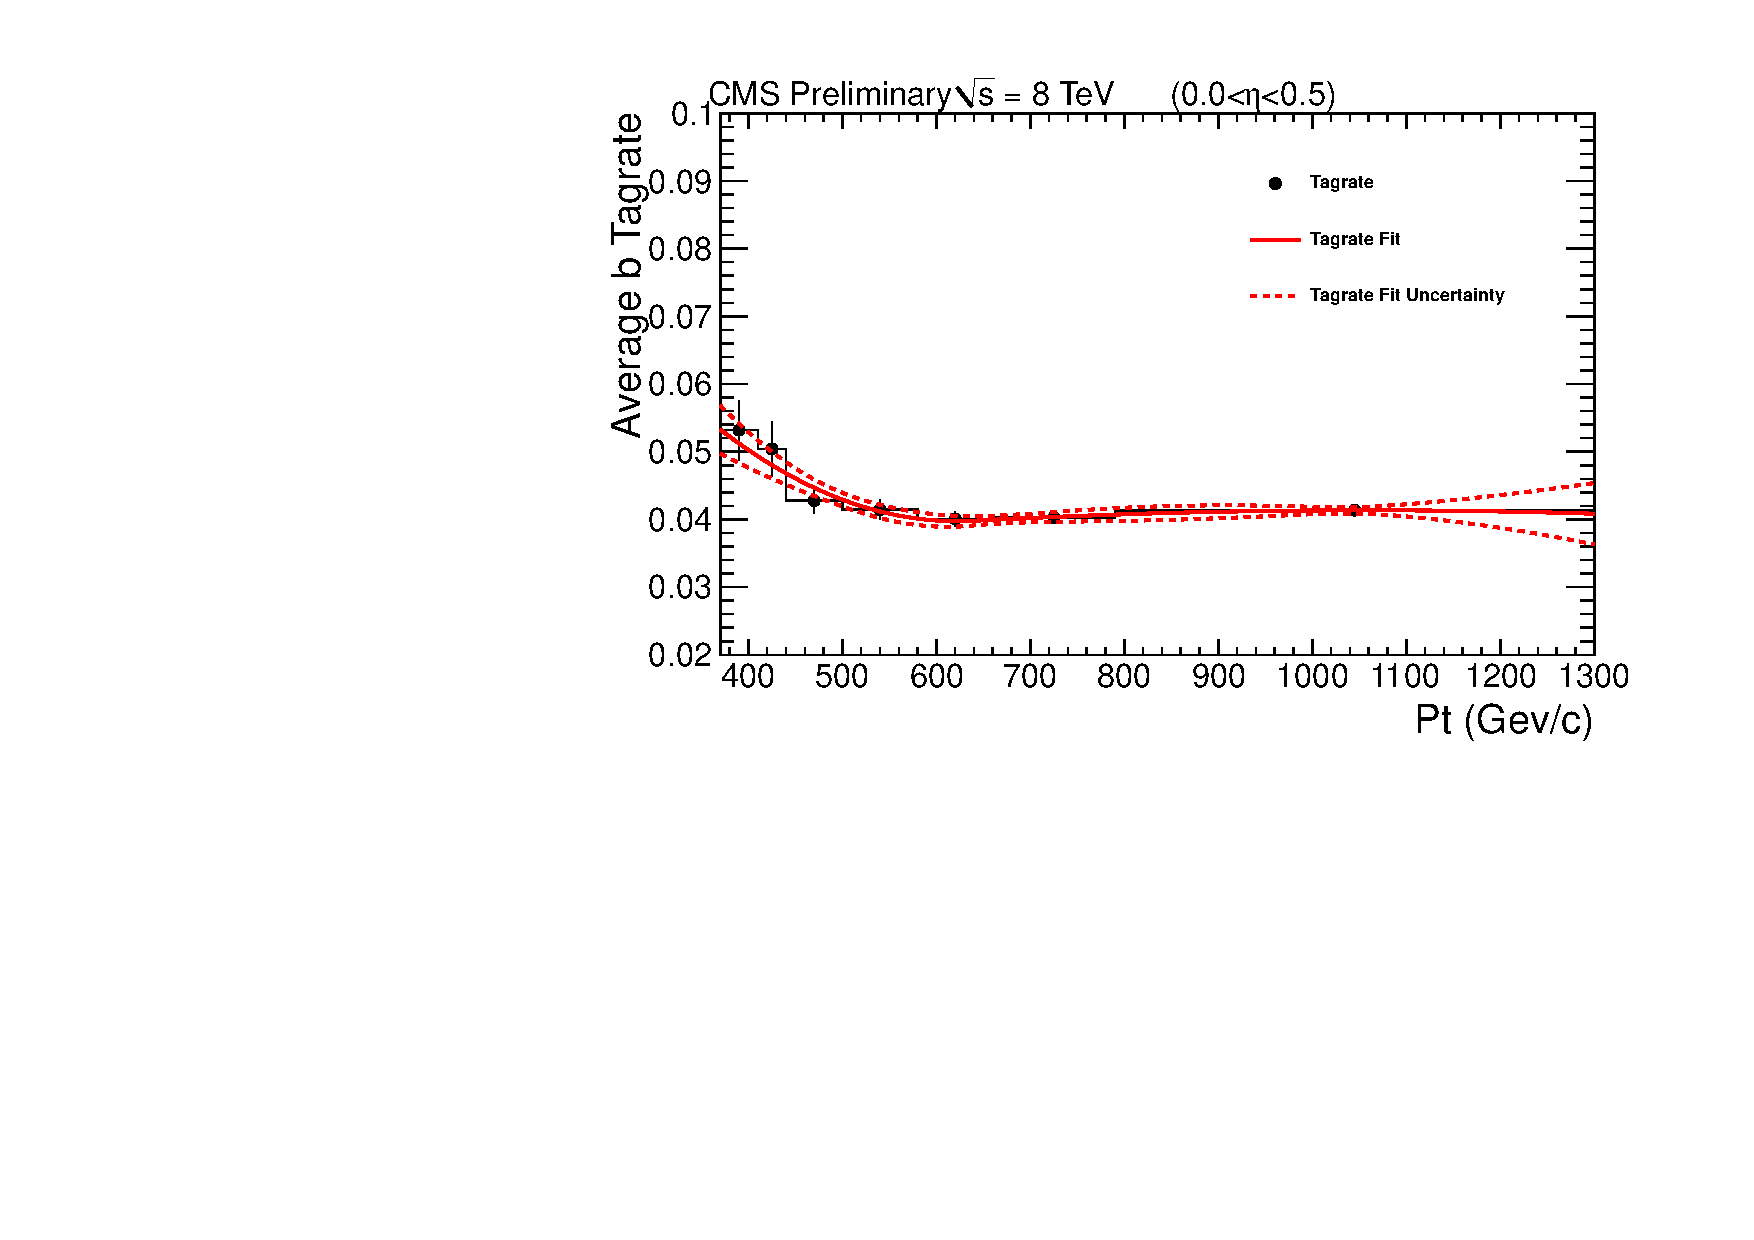
\includegraphics[width=0.75\textwidth]{AN-13-004/figs/tagrateeta1fitBPQCD.pdf}}\\
%\subfigure{\label{figs:tagrateeta2fitBPQCD}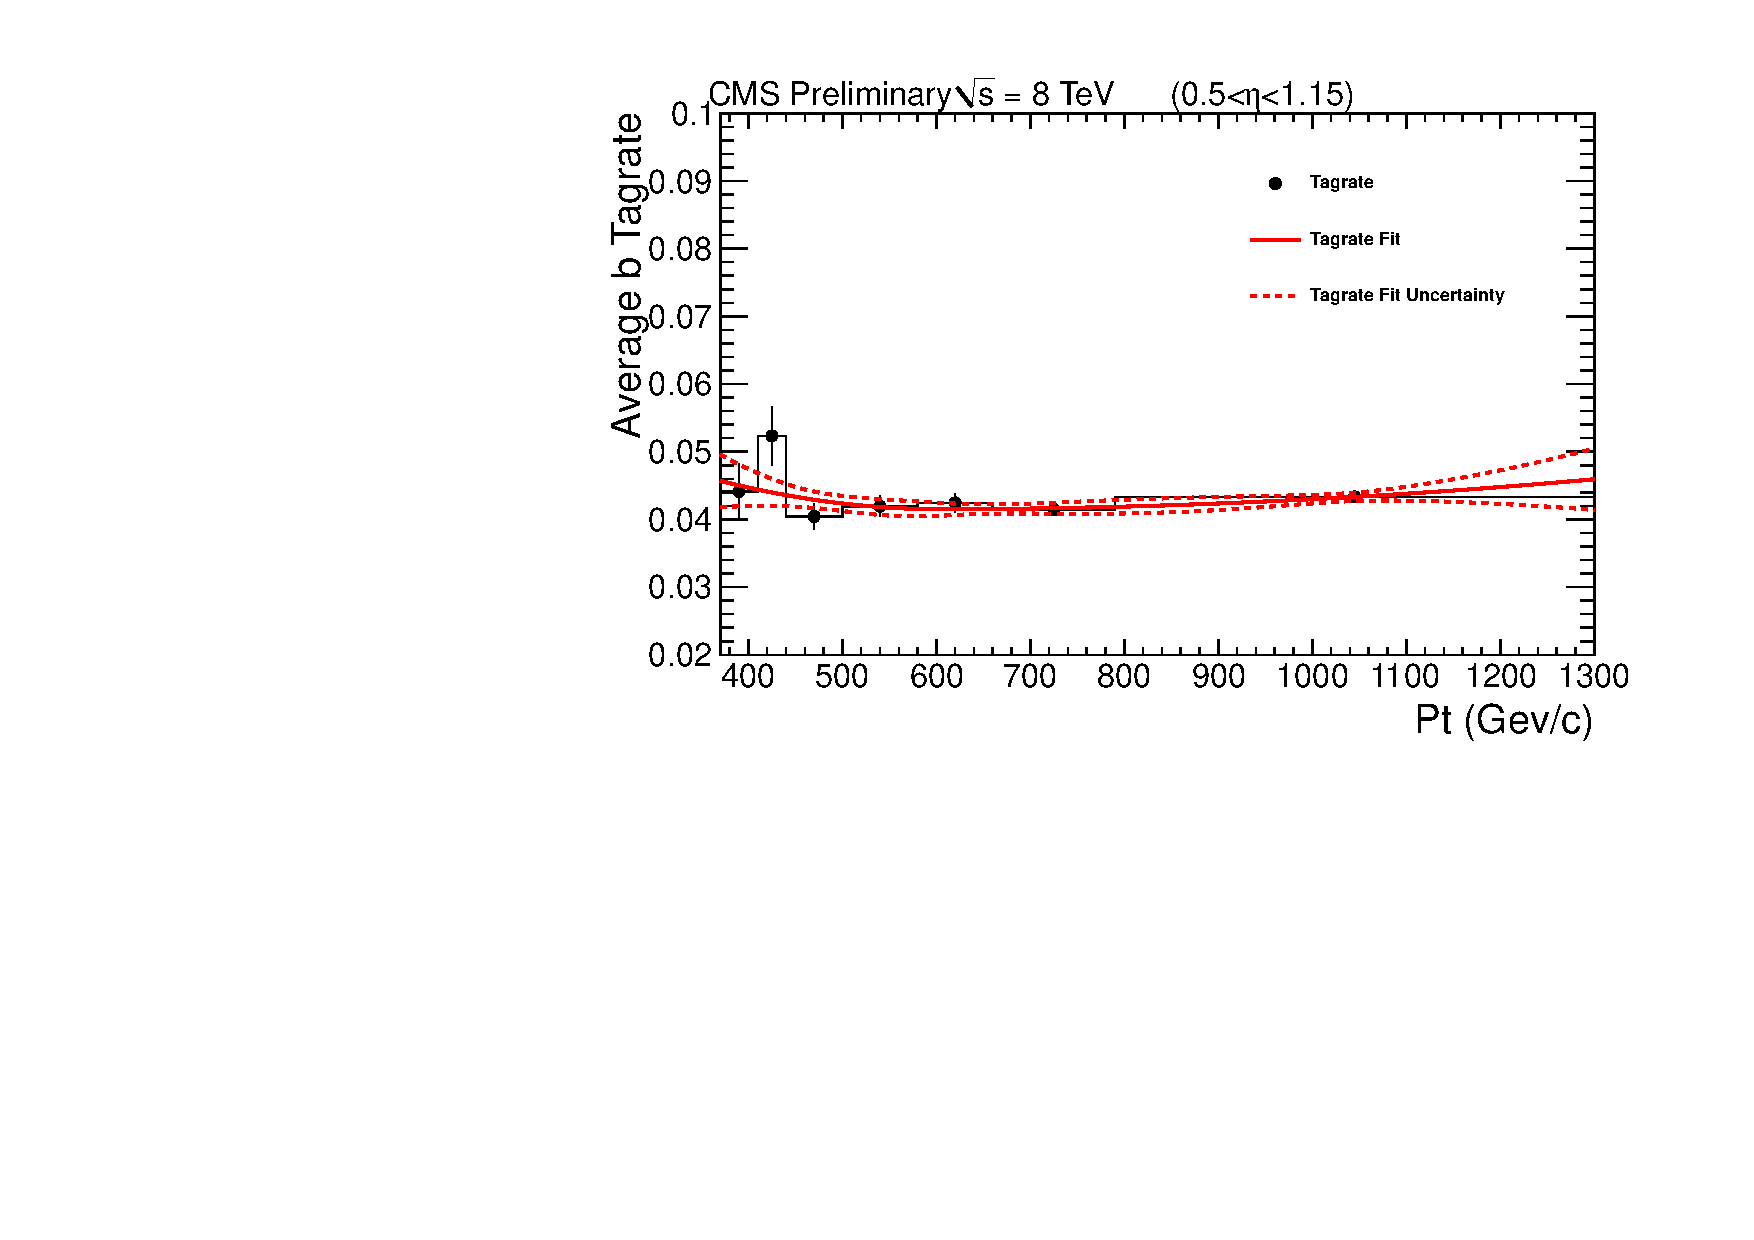
\includegraphics[width=0.75\textwidth]{AN-13-004/figs/tagrateeta2fitBPQCD.pdf}}\\
%\subfigure{\label{figs:tagrateeta3fitBPQCD}\includegraphics[width=0.75\textwidth]{AN-13-004/figs/tagrateeta3fitBPQCD.pdf}}
%\caption{
%QCD MC $\pt$ parameterized tagrate from
%(a) Low $\eta$ region  
%(b) Transition $\eta$ region 
%(c) High $\eta$ region 
%the average b-tagging rate is shown in black, the polynomial fit is shown in red, and the propagated errors from the fit are shown as a red dashed line.}
%\label{figs:tagrateetafitQCD}
%\end{center}
%\end{figure}

%\begin{figure}[htcb]
%\begin{center}
%\subfigure{\label{figs:tagrateeta1QCD_withSR}\includegraphics[width=0.75\textwidth]{AN-13-004/figs/tagrateeta1QCD_withSR}}\\
%\subfigure{\label{figs:tagrateeta2QCD_withSR}\includegraphics[width=0.75\textwidth]{AN-13-004/figs/tagrateeta2QCD_withSR}}\\
%\subfigure{\label{figs:tagrateeta3QCD_withSR}\includegraphics[width=0.75\textwidth]{AN-13-004/figs/tagrateeta3QCD_withSR}}
%\caption{
%QCD MC $\pt$ parameterized tagrate comparison to the signal region from
%(a) Low $\eta$ region  
%(b) Transition $\eta$ region 
%(c) High $\eta$ region 
%the average b-tagging rate from the Signal Region is shown in black, the average b-tagging rate from the Sideband is shown in red.}
%\label{figs:tagrateetaQCD_withSR}
%\end{center}
%\end{figure}

%\begin{figure}[htcb]
%\begin{center}
%\subfigure{\label{figs:MtbvsBkgQCDEO}\includegraphics[width=1.0\textwidth]{AN-13-004/figs/MtbvsBkgQCDEO.pdf}}\\
%\subfigure{\label{figs:MtbvsBkgsemilog_QCDEO}\includegraphics[width=1.0\textwidth]{AN-13-004/figs/MtbvsBkgsemilog_QCDEO.pdf}}
%\caption{
%QCD Monte Carlo background estimation closure test.  The background estimation is extracted from the tagrates shown in Figure\ref{figs:tagrateetafitQCD}.  The full selection is shown in black, 
%the background estimation is shown in yellow, and the errors from the background estimation are shown as a red dashed line.  Top and bottom plots are the same but on linear and log y-axis scale. }
%\label{figs:QCDClosure}
%\end{center}
%\end{figure}

\section{Sideband Closure}
\label{sec:secondsideband}
In order to investigate the applicability and versatility of the QCD background estimation in data, we apply the average b-tagging rate to sideband regions of our top tagging selection.  First, we define the following sideband:

\begin{itemize}
\item {\bf Jet Mass}  $\mathrm{\boldmath 140~\GeV < m_{\text{jet}} < 250~\GeV}$ 
\item {\bf Number of Subjets}  $\mathrm{\boldmath N_{\text{subjets}} > 2}$ 
\item {\bf Minimum Pairwise Mass} $\mathrm{\boldmath m_{\text{min}} \leq 50~\GeV}$ 
\item {\bf N-subjettiness} $\mathrm{\boldmath \tau_3/\tau_2 \geq 0.55}$ 
\item {\bf Subjet b-Tagging} $\mathrm{\boldmath SJ_{\text{CSVMAX}} \geq 0.679}$ 
\end{itemize}
This region lies outside of the signal region and sideband used for average b-tagging rate determination.  
The selection also has a very low yield of $\ttbar$, making it ideal for investigating the QCD background contribution.  
The average b-tagging rate used for this closure test is extracted from the same sideband as the signal region, and applied to pre-b-tagged events.  The closure test can be seen in Figure \ref{figs:NewMtbSB2}.

\begin{figure}[Htcb]
\centering
\subfigure{\label{figs:NewMtbSB21}\includegraphics[width=.9\textwidth]{AN-13-004/figs/NewMtbSB2.pdf}}\\
\subfigure{\label{figs:NewMtbSB22}\includegraphics[width=.9\textwidth]{AN-13-004/figs/NewMtbSB2semilog.pdf}}
\caption{A plot of $M_{tb}$ in the control region defined by inverting the minimum pairwise mass and N-subjettiness cuts used in the full selection.  The top and bottom plots are the same but with linear and log y-axis scale.}
\label{figs:NewMtbSB2}
\end{figure}

Additionally, we can define the following sideband 
\begin{itemize}
\item {\bf Jet Mass}  $\mathrm{\boldmath 140~\GeV < m_{\text{jet}} < 250~\GeV}$ 
\item {\bf Number of Subjets}  $\mathrm{\boldmath N_{\text{subjets}} > 2}$ 
\item {\bf Minimum Pairwise Mass} $\mathrm{\boldmath m_{\text{min}} > 50~\GeV}$ 
\item {\bf N-subjettiness} $\mathrm{\boldmath \tau_3/\tau_2 < 0.55}$ 
\item {\bf Subjet b-Tagging} $\mathrm{\boldmath SJ_{\text{CSVMAX}} \leq 0.679}$ 
\end{itemize}
The closure test can be seen in Figure \ref{figs:NewMtbSB3}.

\begin{figure}[Htcb]
\centering
\subfigure{\label{figs:NewMtbSB31}\includegraphics[width=.9\textwidth]{AN-13-004/figs/NewMtbSB3.pdf}}\\
\subfigure{\label{figs:NewMtbSB32}\includegraphics[width=.9\textwidth]{AN-13-004/figs/NewMtbSB3semilog.pdf}}
\caption{A plot of $M_{tb}$ in the control region defined by inverting the subjet b tagging cut used in the full selection.  The top and bottom plots are the same but with linear and log y-axis scale.}
\label{figs:NewMtbSB3}
\end{figure}

\section{Deriving the normalization of the SM $\ttbar$ production}
\label{sec:ttbarsideband}
In order to study the contribution from $\ttbar$ to tbe full background estimate, we turn to a sideband defined by inverting the b candidate mass requirement in the signal region.
This selection has an amplified $\ttbar$ fraction and is statistically independent from all other sidebands in the analysis.  
This makes the selection ideal for extracting the $\ttbar$ fraction in data.  
In order to extract this fraction, we compare the data-driven QCD background and $\ttbar$ Monte Carlo expectation to the selection in data.  

We perform a template fit to the invariant mass of the b 
candidate, using scaled $\ttbar$ Monte Carlo as one template, and the QCD background prediction as the other.  The fit allows
the QCD background template to move only within its errors, whereas the normalization on $\ttbar$ is unconstrained. 
The optimal parameterization for this fit is in a variable that has distinctly different shapes in $\ttbar$ and QCD.  
We therefore use the b candidate mass, which minimizes the correlation between the QCD and $\ttbar$ templates within the fit. The fit can be seen in Figure \ref{figs:ttbarfit}.  For this maximum likelihood fit we use the Theta package.

Additionally, the fit implements the $\ttbar$ subtraction in the QCD estimate by fitting un-subtracted QCD to the $\ttbar$ full selection.  The output of the fitter is then corrected by  
(1+S/F), where S/F is the ratio of the number of events in $\ttbar$ subtracted selection to the $\ttbar$ full selection. 

This study suggests after all scale factors applied in the analysis, the $\ttbar$ contribution needs to be amplified by $1.23 \pm 0.24$.  
This normalization is used for all $\ttbar$ distributions in the analysis, and the uncertainty is then the full normalization uncertainty for $\ttbar$.

\begin{figure}[htcb]
\centering
\includegraphics[width=1.0\textwidth]{AN-13-004/figs/ttbarfittingfromthetatmass}
\caption{b candidate mass as extracted from the b candidate mass inverted sideband.  Pre fraction fit (left) and post fraction fit (right).}
\label{figs:ttbarfit}
\end{figure}





\section{Data Results}
After closure of the background estimation procedure within control regions, 
we first apply the background estimate to a loose selection that contains all of the full selection cuts with the exception of subjet 
b-tagging and N-subjettiness.  The agreement using this selection can be seen in figure \ref{figs:CMSTTonlyMtbvsBkg1}.

\begin{figure}[htcb]
\begin{center}
\subfigure{\label{figs:CMSTTonlyMtbvsBkg_BifPoly_fit}\includegraphics[width=0.7\textwidth]{AN-13-004/figs/CMSTTonlyMtbvsBkg_BifPoly_fit.pdf}}\\
\subfigure{\label{figs:CMSTTonlyMtbvsBkgsemilog_BifPoly_fit}\includegraphics[width=0.7\textwidth]{AN-13-004/figs/CMSTTonlyMtbvsBkgsemilog_BifPoly_fit.pdf}}
\caption{
A plot of the full selection before N-subjettiness and subjet b-tagging discrimination.   
Here we investigate the data-background agreement in a loose selection before looking at the full top tagging selection.  Top and bottom plots are the same but with linear and log y-axis scale.}
\label{figs:CMSTTonlyMtbvsBkg1}
\end{center}
\end{figure}

After observing agreement is the loose selection, we investigate the full selection.  The final results are shown in Figure \ref{figs:MtbvsBkg1}.  We proceed to compute 
limits on the $\wpr$ cross-section.  Background estimation of selected relevant variables can be seen in 
Figures \ref{figs:kinplotsdata1} and \ref{figs:kinplotsdata2}.

\begin{figure}[htcb]
\begin{center}
\subfigure{\label{figs:MtbvsBkg_BifPoly_fit}\includegraphics[width=0.7\textwidth]{AN-13-004/figs/MtbvsBkg_BifPoly_fit.pdf}}\\
\subfigure{\label{figs:MtbvsBkgsemilog_BifPoly_fit}\includegraphics[width=0.7\textwidth]{AN-13-004/figs/MtbvsBkgsemilog_BifPoly_fit.pdf}}
\caption{
A plot of the full selection comparing data, signal and background.  
The single top contribution is not considered when setting limits.  
The normalization for the signal samples is set to a cross-section of 0.2 pb.  Top and bottom plots are the same but on linear and log y-axis scale.}
\label{figs:MtbvsBkg1}
\end{center}
\end{figure}

\begin{figure}[htcb]
\centering
\includegraphics[width=.7\textwidth]{AN-13-004/figs/KinPlots_Data1.pdf}
\caption{Background estimation of kinematic variables.  The error bars shown are from the three primary sources; uncertainty on the fit, choice of fit, $\ttbar$ normalization, and $\ttbar$ $Q^2$ uncertainty}
\label{figs:kinplotsdata1}
\end{figure}  
\clearpage

\begin{figure}[htcb]
\centering
\includegraphics[width=.7\textwidth]{AN-13-004/figs/KinPlots_Data2.pdf}
\caption{Background estimation of kinematic variables.  The error bars shown are from the three primary sources; uncertainty on the fit, choice of fit, $\ttbar$ normalization, and $\ttbar$ $Q^2$ uncertainty}
\label{figs:kinplotsdata2}
\end{figure}  
\clearpage


\clearpage
\newpage
\section{Systematic Uncertainties}
\label{sec:systematics}
Various systematics are taken into account, both 
on our expected signal and background estimate. Some systematic uncertainties will affect only the normalization of certain event rates, 
and are reported as overall normalization uncertainties. Other systematics affect the shapes of the reconstructed signal or backgrounds, as well as their normalization.  The
Systematic uncertainties that are used in the analysis are summarized in table \ref{table:nuisance}.% All systematic effects are listed in Table \ref{table:systeffects}.

%\begin{sidewaystable}
%\begin{center}
%\begin{small}
%\begin{tabular}{| c || c || c | c | c  c  c  c  c  c  c  c |}
%\hline
%& \textbf{Process:} & $t\overline{t}$ & QCD & & & & & & & &\\
%& \textbf{$W^\prime$ Mass Point:} & & & 1300 & 1500 & 1700 & 1900 & 2100 & 2300 & 2700 & 3100  \\
%\hline
%\textbf{Systematic} & \textbf{Variation ($\%$)} & \multicolumn{9}{c}{\textbf{Effect of Systematic} (\%)} \\ 
%\hline
%Luminosity & $\pm 4.4$ & 4.4 &  & 4.4 & 4.4 & 4.4 & 4.4 & 4.4 & 4.4 & 4.4 & 4.4 \\
%Subjet Scale Factor & $\pm 5$ & 5 &  & 5 & 5 & 5 & 5 & 5 & 5 & 5 & 5 \\
%$t\overline{t}$ cross-section & $\pm 50$ & 50 & & & & & & & & & \\
%b-tagging & see text & 7 & & 8 & 8 & 9 & 9 & 11 & 11 & 12 & 10  \\
%Trigger Efficiency & see text & 7 & & 1 & $<1$ & $<1$ & $<1$ & $<$1 & $<1$ & $<1$ & $<1$  \\
%Jet Energy Scale$^{up}_{down}$ & $\pm 5$ & $^{22}_{20}$ & & $^{7}_{11}$ & $^{1}_{4}$ & $^{1}_{2}$ & $^{12}_{0.1}$ & $^{4}_{1}$ & $^{4}_{1}$ & $^{4}_{1}$ & $^{0.5}_{3}$  \\
%QCD Systematic & see text & & 4 & & & & & & & &  \\
%\hline
%Number of Events& & 1042 & 17901 & 579 & 274 & 118 & 51 & 22 & 10 & 2 & 1 \\
%\hline
%\end{tabular}
%\caption{Effect of systematics listed in Section \ref{sec:systematics}, computed over the entire mass-range.  The b-tagging, Jet Energy Scale, and Trigger uncertainties have non negligible 
%shape based effects that must be taken into account. Note: the $2\%$ b-tagging systematic derived in Section \ref{sec:btagging} is included in the b-tagging line above.}
%\label{table:systeffects}
%\end{small}
%\end{center}
%\end{sidewaystable}

\subsection{Jet Energy Scale}
We evaluate the effect of uncertainty on the jet energy scale on samples derived from MC simulation.  
To do so, we vary the jet four-momentum up and down by the jet energy 
scale uncertainty, which we take to be $3\%$. We include $\pt$ and $\eta$ dependent corrections to the 
jet energies, as well as uncertainties from the difference in measured and simulated $W$ masses \cite{ZP8TeV}. 

Varying the jet momentum can cause a jet to fall below or rise above the $\pt$ cut in the analysis, thus shifting the invariant 
mass spectrum of the signal and reconstructed $\ttbar$ samples. Figure \ref{figs:ttbarJES} shows the systematic shapes from the 
jet energy scale on the $\ttbar$ distribution.  Jet Energy scale variation on signal MC is shown in Figure \ref{figs:signalJES} for 1300$~\GeV$,
 1900$~\GeV$, and 2300$~\GeV$ mass points.

\subsection{Trigger}
We include an uncertainty based on the measured trigger efficiency for all MC Samples. The trigger efficiency is discussed in Section \ref{sec:trigger}. 
To obtain shape systematics from this effect, we vary the trigger by half the trigger \textit{in}efficiency. The effects of this on the $t\overline{t}$ 
distribution is shown in Figure \ref{figs:ttbartrig}. Trigger weighting on signal MC is shown in Figure \ref{figs:signaltrig} for 1300$~\GeV$,
 1900$~\GeV$, and 2300$~\GeV$ mass points.  The uncertainty is low in the mass range of interest for limit setting.

\subsection{Jet Energy Resolution}
\label{sec:JER}
We apply a systematic due to the known differences in jet energy resolution in data and simulation.  We use $\eta$ dependent smearing (see \cite{ZP8TeV}) as recommended by the JER group.  
We apply this systematic uncertainty to the $t\overline{t}$ distribution 
(as seen in Figure \ref{figs:ttbarJER}).  Jet Energy Resolution variation on signal MC is shown in Figure \ref{figs:signalJER} for 1300$~\GeV$,
 1900$~\GeV$, and 2300$~\GeV$ mass points. 

\subsection{Jet Angular Resolution}
A smearing of $10\%$ is assumed on $\eta$ and $\phi$ and shape uncertainties are generated by considering smearing $10\%$ 
lower and higher. We apply this systematic uncertainty to the $\ttbar$ distribution (as seen in Figure \ref{figs:ttbarJAR} ). Jet Angular Resolution 
variation on signal MC is shown in Figure \ref{figs:signalJAR} for 1300$~\GeV$,
 1900$~\GeV$, and 2300$~\GeV$ mass points.  The effect is very small and thus not considered in setting limits.

\subsection{PDF Uncertainty}
The uncertainty in the parton distribution function used for MC sample generation is investigated.  We take the average of the $\pm$1$\sigma$ eigenvalue 
variation of the pdf master equations \cite{Bourilkov:2006cj} 
for the NNPDF, MSTW2008nnlo, and CT10 pdf sets to weight the signal and $\ttbar$ MC samples and investigate the impact on the full selection.  The PDF set 
that provides the maximum uncertainty is then used for the $\pm$1$\sigma$ PDF uncertainty.  For $\ttbar$ and signal this set is NNPDF. PDF 
variation on signal MC is shown in Figure \ref{figs:signalPDF} for 1300$~\GeV$,
 1900$~\GeV$, and 2300$~\GeV$ mass points.  PDF variation on $\ttbar$ MC is shown in Figure \ref{figs:ttbarPDF}.  The effect is very small and thus not considered in setting limits.

\subsection{Pileup}
A study of pileup uncertainty is conducted by varying the minimum bias cross-section by 5\% as a measure of systematic uncertainty.  The results 
can be seen in figure \ref{figs:signalPU}.  The effect is very small and thus not considered in setting limits.

\subsection{b-Tagging Scale Factor Uncertainty}
\label{sec:btagunc}
The uncertainty in the b-tagging scale factor described in Section \ref{sec:btagging} is applied based on the b candidate pt.  The binning and associated errors 
listed below are the suggested EPS13 prescription generated from measurements in both muon-jet and ttbar data representing 20$~\fbinv$ of integrated 
luminosity.  The absolute uncertainty on $\mathrm{SF_b}$ for a b candidate jet within the listed $\pt$ range is applied as shown in table \ref{table:btaggingerrors} 
for $\pt < 800~\GeV$.  B candidate jets with $\pt > 800~\GeV$ are assigned an uncertainty equal to twice the listed value for $600~\GeV < \pt < 800~\GeV$

\begin{table}
\begin{center}
\begin{tabular}{l|c} 
\hline\hline
\bf{$\pt$ range } & \bf{Absolute Error on $\mathrm{SF_b}$} \\
\hline\hline
$320~\GeV < \pt < 400~\GeV$ & 0.0313175 \\
$400~\GeV < \pt < 500~\GeV$ & 0.0415417 \\
$500~\GeV < \pt < 600~\GeV$ & 0.0740446 \\
$600~\GeV < \pt < 800~\GeV$ & 0.0596716 \\
\hline
\end{tabular}
\end{center}
\caption{Absolute Error applied to the b-tagging Scale Factor}
\label{table:btaggingerrors}
\end{table}


%\clearpage

\subsection{$\mathrm{Q^2}$ Scale Uncertainty}
We use additional $\ttbar$ samples generated with twice and half the nominal $\mathrm{Q^2}$ 
scale used in the $\ttbar$ samples listed in table \ref{table:datasets}.  These samples vary the renormalization and factorization scales to account for 
missing higher order corrections in our simulation.  Figure \ref{figs:q2scale} shows the shape based uncertainty due to this effect.

\begin{figure}[htcb]
\begin{center}
\includegraphics[width=0.7\textwidth]{AN-13-004/figs/TTbar_Q2Scale}
\caption{
$\mathrm{Q^2}$ systematic variation for $\ttbar$ MC 
}
\label{figs:q2scale}
\end{center}
\end{figure}

\subsection{$\ttbar$ $\pt$ Re-weighting}
The uncertainty related to the $\pt$ re-weighting scheme presented in Section \ref{sec:ttptrw} is taken as the difference between the weighted and unweighted $\ttbar$ spectrum.
%However, this scheme has both a normalization and shape based effect.  Due to the fact that we extract the $\ttbar$ normalization uncertainty (see Section \ref{sec:ttbarsideband}), 
%we normalize the up and down systematic to the nominal $\pt$ re-weighting and use this in limit setting.
This uncertainty can be seen in figure \ref{figs:ptreweight}.  This is the dominant uncertainty for $\ttbar$. 

\begin{figure}[htcb]
\begin{center}
\includegraphics[width=0.7\textwidth]{AN-13-004/figs/TTbar_PTReweighting}
\caption{
$\pt$ re-weighting systematic variation for $\ttbar$ MC 
}
\label{figs:ptreweight}
\end{center}
\end{figure}

\subsection{Normalization Uncertainties}
As mentioned in Section \ref{sec:ttbarsideband}, the uncertainty due to the overall normalization scale factor used for $\ttbar$ is extracted from data and is $19\%$.   

We must apply a $13\%$ uncertainty on the top tagging scale factor described in Section \ref{sec:subjetSF} to signal MC events due to uncertainty in the difference in subjet efficiency from data to MC.

As mentioned in Section \ref{sec:btagging}, we add a $2\%$ uncertainty to the signal estimates from the AK5 vs. CA8 scale factor on b-tagging efficiency. 

We also include a $2.6\%$ uncertainty in the luminosity for the signal MC \cite{CMS-PAS-LUM-13-001}. 


\clearpage
\subsection{Uncertainties related to the QCD Background Estimate}
We use the result of the fit to the average b-tagging rate (see Section \ref{sec:backgroundEstimation}) to weight 
pre b-tagged events in order to create the QCD background estimate.  Uncertainties in
the fitting algorithm and statistical uncertainties in the sideband
are taken into account (see figure \ref{figs:tagrateetafit}).
Statistical uncertainties in the pre b tagged signal region are also
taken into account.

\subsubsection{Choice of the functional form for the average b-tagging rate}
\label{sec:choiceoffit}
The functional form used is a bifurcated polynomial.
However there is a systematic uncertainty associated with this choice.
The uncertainties due to this effect are taken into account by
studying alternative functional forms seen in figure
\ref{figs:BKGFITCOMP}.  The background estimation from these
alternative fits are seen in figure \ref{figs:BKGCOMP}.  The
uncertainty due to the choice of fit is taken as the Mean Squared
Error of these alternative backgrounds bin by bin and can be seen in
figure \ref{figs:BKGERR}.  


\subsubsection{Two-dimensional  vs. three-dimensional parameterization of the average b-tagging rate}
\label{sec:paramerrors1}
Additionally, we place an uncertainty on the inability of the
background estimate to capture all kinematic correlations through the
parameterization of the average b-tagging rate in $\pt$ and $\eta$.
This uncertainty is calculated by investigating a parameterization in
$\pt$ $\eta$ and $\mathrm{M_{tb}}$.  We define $P_i$ as the average b-tagging
rate described in Section \ref{sec:backgroundEstimation} in one
$\eta$ bin and $P_{ij}$ as the average b-tagging rate if parameterized
with $\mathrm{M_{tb}}$ as well.  $P_{ij}$ can be seen in
figure \ref{figs:sb2deta}.  Each bin in $P_i$ can be thought of as a
column average over all $\mathrm{M_{tb}}$ bins per $\pt$ bin.  If $P_{ij}$ a
function of $\mathrm{M_{tb}}$ (index $j$) is not constant, then averaging over
$P_{ij}$ over $j$ while projecting onto $\mathrm{M_{tb}}$ axis to obtain the
QCD background estimate can result in a bias.  For more in-depth
discussion on this effect, please see Section \ref{sec:qcdpunc}.

We assess the approximate size of the uncertainty due to our choice of
parameterization by explicitly comparing the three-dimensional and
two-dimensional background estimates in the sideband.  Using these two
parameterizations, the uncertainty in the $\mathrm{M_{tb}}$ distribution due to
parameterization is approximately $\displaystyle\sum\limits_{j=0}^n
m_{ij}$($P_{ij}-P_i$) where $m_{ij}$ refers to the number of pretag
events for a bin in $\pt$ and $\mathrm{M_{tb}}$.  Fig. \ref{figs:PARAMERROR}
shows the uncertainty due to this effect. These uncertainties are
taken in quadrature to produce an overall uncertainty in the data
derived background estimate that is applied in a shape based manner in
the limit-setting macro.

\begin{sidewaystable}
\begin{center}
\bf{Rate Effects of Systematic Uncertainties}\\
\scalebox{0.5}{
\begin{tabular}{c||c|c|c|c|c|c|c|c|c|c|c}
\hline\hline
\bf{Sample} & \bf{CA btag SF}  & \bf{QCD total} & \bf{b-tagging}  & \bf{JES}  & \bf{Lumi}  & \bf{$\pt$ Reweight} & \bf{JER}  & \bf{$\mathrm{Q^2}$}  & \bf{Subjet SF}  & \bf{Trigger}  & \bf{$\ttbar$ Norm} \\
\hline\hline
qcd & --- & +9.05,-8.94 & --- & --- & --- & --- & --- & --- & --- & --- & ---\\
ttbar & --- & --- & +4.49,-4.49 & -0.42,+0.49 & +16.49,-15.27 & --- & +21.77,-14.96 & -74.04,+77.89 & --- & +0.30,-0.30 & +19.00,-15.97\\
1300 & +2.00,-1.96 & --- & +6.08,-6.08 & -0.27,+0.29 & +2.06,-3.85 & +2.60,-2.53 & --- & --- & +12.50,-11.11 & +0.06,-0.06 & ---\\
1500 & +2.00,-1.96 & --- & +6.48,-6.48 & -0.03,+0.17 & -0.29,-0.19 & +2.60,-2.53 & --- & --- & +12.50,-11.11 & +0.02,-0.02 & ---\\
1700 & +2.00,-1.96 & --- & +6.94,-6.94 & -0.02,+0.12 & -1.27,+1.17 & +2.60,-2.53 & --- & --- & +12.50,-11.11 & +0.01,-0.01 & ---\\
1900 & +2.00,-1.96 & --- & +8.12,-8.12 & -0.08,+0.02 & -1.76,+1.78 & +2.60,-2.53 & --- & --- & +12.50,-11.11 & +0.01,-0.01 & ---\\
2100 & +2.00,-1.96 & --- & +9.39,-9.39 & +0.06,-0.05 & -1.81,+1.61 & +2.60,-2.53 & --- & --- & +12.50,-11.11 & +0.01,-0.01 & ---\\
2300 & +2.00,-1.96 & --- & +10.01,-10.01 & +0.02,+0.09 & -1.76,+1.24 & +2.60,-2.53 & --- & --- & +12.50,-11.11 & +0.02,-0.02 & ---\\
2700 & +2.00,-1.96 & --- & +9.49,-9.49 & -0.25,+0.08 & -0.33,+0.47 & +2.60,-2.53 & --- & --- & +12.50,-11.11 & +0.04,-0.04 & ---\\
\hline
\end{tabular}
}
\end{center}
\caption{Rate effects of the systematic uncertainties as extracted from Theta.  The numbers listed under sample specify $\wpr_R$ signal MC mass.}
\label{table:nuisance}
\end{sidewaystable}


\begin{figure}[htcb]
\begin{center}
\includegraphics[width=0.4\textwidth]{AN-13-004/figs/Signal_M1300_PtScaling}
\includegraphics[width=0.4\textwidth]{AN-13-004/figs/Signal_M1900_PtScaling}
\includegraphics[width=0.4\textwidth]{AN-13-004/figs/Signal_M2300_PtScaling}
\caption{
Jet Energy Scale systematic variation for Right-handed $\wpr$ MC at the following mass points
(a) $M_{\wpr}$ = 1300$~\GeV$ 
(b) $M_{\wpr}$ = 1900$~\GeV$
(c) $M_{\wpr}$ = 2300$~\GeV$ 
}
\label{figs:signalJES}
\end{center}
\end{figure}

\begin{figure}[htcb]
\begin{center}
\includegraphics[width=0.7\textwidth]{AN-13-004/figs/TTbar_PtScaling}
\caption{Jet Energy Scale systematic variation for $\ttbar$ MC}
\label{figs:ttbarJES}
\end{center}
\end{figure}

\begin{figure}[htcb]
\begin{center}
\includegraphics[width=0.45\textwidth]{AN-13-004/figs/Signal_M1300_TriggerWeighting}
\includegraphics[width=0.45\textwidth]{AN-13-004/figs/Signal_M1900_TriggerWeighting}
\includegraphics[width=0.45\textwidth]{AN-13-004/figs/Signal_M2300_TriggerWeighting}
\caption{
Trigger Weighting systematic variation for Right-handed $\wpr$ MC at the following mass points
(a) $M_\wpr$ = 1300$~\GeV$ 
(b) $M_\wpr$ = 1900$~\GeV$
(c) $M_\wpr$ = 2300$~\GeV$ 
}
\label{figs:signaltrig}
\end{center}
\end{figure}

\begin{figure}[htcb]
\begin{center}
\includegraphics[width=0.7\textwidth]{AN-13-004/figs/TTbar_TriggerWeighting}
\caption{Trigger Weighting systematic variation for $\ttbar$ MC}
\label{figs:ttbartrig}
\end{center}
\end{figure}


\begin{figure}[htcb]
\begin{center}
\includegraphics[width=0.45\textwidth]{AN-13-004/figs/Signal_M1300_PtSmearing}
\includegraphics[width=0.45\textwidth]{AN-13-004/figs/Signal_M1900_PtSmearing}
\includegraphics[width=0.45\textwidth]{AN-13-004/figs/Signal_M2300_PtSmearing}
\caption{
Jet Energy Resolution systematic variation for Right-handed $\wpr$ MC at the following mass points
(a) $M_{\wpr}$ = 1300$~\GeV$ 
(b) $M_{\wpr}$ = 1900$~\GeV$
(c) $M_{\wpr}$ = 2300$~\GeV$ 
}
\label{figs:signalJER}
\end{center}
\end{figure}

\begin{figure}[htcb]
\begin{center}
\includegraphics[width=0.7\textwidth]{AN-13-004/figs/TTbar_PtSmearing}
\caption{Jet Energy Resolution systematic variation for $\ttbar$ MC}
\label{figs:ttbarJER}
\end{center}
\end{figure}

\begin{figure}[htcb]
\begin{center}
\includegraphics[width=0.45\textwidth]{AN-13-004/figs/Signal_M1300_EtaScaling}
\includegraphics[width=0.45\textwidth]{AN-13-004/figs/Signal_M1900_EtaScaling}
\includegraphics[width=0.45\textwidth]{AN-13-004/figs/Signal_M2300_EtaScaling}
\caption{
Jet Angular Resolution systematic variation for Right-handed $\wpr$ MC at the following mass points
(a) $M_\wpr$ = 1300$~\GeV$ 
(b) $M_\wpr$ = 1900$~\GeV$
(c) $M_\wpr$ = 2300$~\GeV$ 
}
\label{figs:signalJAR}
\end{center}
\end{figure}

\begin{figure}[htcb]
\begin{center}
\includegraphics[width=0.7\textwidth]{AN-13-004/figs/TTbar_EtaScaling}
\caption{Jet Angular Resolution systematic variation for $\ttbar$ MC}
\label{figs:ttbarJAR}
\end{center}
\end{figure}

\begin{figure}[htcb]
\begin{center}
\includegraphics[width=0.45\textwidth]{AN-13-004/figs/Signal_M1300_PdfScaleNNPDF23.pdf}
\includegraphics[width=0.45\textwidth]{AN-13-004/figs/Signal_M1900_PdfScaleNNPDF23.pdf}
\includegraphics[width=0.45\textwidth]{AN-13-004/figs/Signal_M2300_PdfScaleNNPDF23.pdf}
\caption{
PDF systematic variation for Right-handed $\wpr$ MC at the following mass points
(a) $M_\wpr$ = 1300$~\GeV$ 
(b) $M_\wpr$ = 1900$~\GeV$
(c) $M_\wpr$ = 2300$~\GeV$ 
}
\label{figs:signalPDF}
\end{center}
\end{figure}

\begin{figure}[htcb]
\begin{center}
\includegraphics[width=0.7\textwidth]{AN-13-004/figs/TTbar_PdfScaleNNPDF23.pdf}
\caption{PDF systematic variation for $\ttbar$ MC}
\label{figs:ttbarPDF}
\end{center}
\end{figure}

\begin{figure}[htcb]
\begin{center}
\includegraphics[width=0.45\textwidth]{AN-13-004/figs/Signal_M1300_PileupReweighting}
\includegraphics[width=0.45\textwidth]{AN-13-004/figs/Signal_M1900_PileupReweighting}
\includegraphics[width=0.45\textwidth]{AN-13-004/figs/Signal_M2300_PileupReweighting}
\caption{
Pileup systematic variation for Right-handed $\wpr$ MC at the following mass points
(a) $M_{\wpr}$ = 1300$~\GeV$ 
(b) $M_{\wpr}$ = 1900$~\GeV$
(c) $M_{\wpr}$ = 2300$~\GeV$ 
}
\label{figs:signalPU}
\end{center}
\end{figure}

%\begin{figure}[htcb]
%\begin{center}
%\includegraphics[width=0.7\textwidth]{AN-13-004/figs/TTbar_PileupReweighting}
%\caption{Pileup systematic variation for $\ttbar$ MC}
%\label{figs:ttbarPU}
%\end{center}
%\end{figure}

\begin{figure}[htcb]
\begin{center}
\includegraphics[width=0.7\textwidth]{AN-13-004/figs/BKGFITCOMPLOGE1.pdf}\\
\includegraphics[width=0.7\textwidth]{AN-13-004/figs/BKGFITCOMPLOGE2.pdf}\\
\includegraphics[width=0.7\textwidth]{AN-13-004/figs/BKGFITCOMPLOGE3.pdf}
\caption{
Alternative fit functions for the average b-tagging rate in $\eta$ regions
(a) Low
(b) Transition
(c) High
}
\label{figs:BKGFITCOMP}
\end{center}
\end{figure}

\begin{figure}[htcb]
\begin{center}
\includegraphics[width=0.7\textwidth]{AN-13-004/figs/BKGCOMP.pdf}\\
\includegraphics[width=0.7\textwidth]{AN-13-004/figs/BKGCOMPLOG.pdf}
\caption{
QCD background estimation from alternative fit functions seen in \ref{figs:BKGFITCOMP}. Top and bottom plots are the same but on linear and log y-axis scale.
}
\label{figs:BKGCOMP}
\end{center}
\end{figure}

\begin{figure}[htcb]
\begin{center}
\includegraphics[width=0.7\textwidth]{AN-13-004/figs/BKGFITERR.pdf}\\
\includegraphics[width=0.7\textwidth]{AN-13-004/figs/BKGFITERRLOG.pdf}
\caption{
Uncertainty on the choice of fit as extracted from the alternative background estimations seen in \ref{figs:BKGCOMP}. Top and bottom plots are the same but on linear and log y-axis scale.
}
\label{figs:BKGERR}
\end{center}
\end{figure}

\begin{figure}[htcb]
\begin{center}
\includegraphics[width=0.7\textwidth]{AN-13-004/figs/TagrateEta1SB2dSB1.pdf}
\includegraphics[width=0.7\textwidth]{AN-13-004/figs/TagrateEta2SB2dSB1.pdf}
\includegraphics[width=0.7\textwidth]{AN-13-004/figs/TagrateEta3SB2dSB1.pdf}
\caption{
Two dimensional parameterization of average b-tagging rate in $p_{T_{b}}$ and $\mathrm{M_{tb}}$.  The x axis binning is identical to the binning in Section \ref{sec:backgroundEstimation}.  
The y-axis is binned adaptively to approximate equivalent statistics over each y-axis bin per x axis bin. 
(a) Low $\eta$ Region
(b) Transition $\eta$ Region
(c) High $\eta$ Region
}
\label{figs:sb2deta}
\end{center}
\end{figure}

\begin{figure}[htcb]
\begin{center}
\includegraphics[width=0.7\textwidth]{AN-13-004/figs/Mtb2dvs1dBE}\\
\includegraphics[width=0.7\textwidth]{AN-13-004/figs/Mtb2dvs1dBEsemilog}
\caption{
Uncertainty on the parameterization choice. Top and bottom plots are the same but on linear and log y-axis scale.
}
\label{figs:PARAMERROR}
\end{center}
\end{figure}



\clearpage
\newpage
\chapter{Results}
\section{Limits}
\label{sec:stats}
We set limits on the production cross-section of 
the $\wpr_R$ boson. We compare the number 
of observed events to the number of events expected given the new physics model. We use the following formula:
\begin{eqnarray}
N_{\textrm{expected}} = \sigma_{\wpr_R} \times B_{\wpr_R \rightarrow tb;W \to hadrons} \times \varepsilon \times \emph{L}
\end{eqnarray}
where $\sigma_{\wpr_R}$ is the $\wpr_R$ cross-section, $B_{\wpr_R \rightarrow \tbbar;W \to hadrons}$ is the branching ratio 
$\wpr_R \to \tbbar$ with the W decay constrained to the hadronic branching fraction, $\varepsilon$ is the signal efficiency corrected by data-driven scale factors and $\emph{L}$ is the integrated luminosity of our dataset. 

We perform a shape analysis using the $\mathrm{M_{tb}}$ distribution.  We use a binned likelihood fit to compare the distribution from the $\wpr$ boson signal 
hypothesis with the Standard Model distribution produced by our background estimation procedure.  

\label{sec:Theta}
To set shape based limits, the Theta package \cite{theta} is used.  We use a Bayesian method to extract 95\% CL upper limits 
on the production of a right-handed $\wpr$ particle.  

A Poisson model is used in each bin of our analysis.  For each bin, the mean of the Poisson distribution is:
\begin{eqnarray}
\mu_i = \sum_k \beta_k \times T_{k,i}
\end{eqnarray}
here, k includes the signal and background models, and T represents the fraction of events expected for each process $k$ in bin $i$.

The likelihood function is then:
\begin{eqnarray}
L(\beta_k) = \prod^{N_{bins}}_i \frac{\mu_i \times e^{-\mu_i}}{N^{data}_i!}
\end{eqnarray}
Where $\mu_i$ is the mean of the Poisson distribution in bin $i$, given in terms of $T$, the number of events expected from the process $k$.

The Theta package performs pseudoexperiments to calculate 68\% and 95\% upper bounds on the limit bands.  
The pseudoexperiments take into account systematic effects as nuisance parameters.  These nuisance parameters 
are varied within their uncertainties and the posterior is refitted for each pseudoexperiment.  

The uncertainty in the jet energy scale, $Q^2$ scale, $\pt$ re-weighting, trigger, $SF_b$, QCD background uncertainties, and jet energy resolution are taken 
as shape based uncertainties, and the other sources of uncertainty are taken as overall normalizations.  

The limits from Theta are shown in Figure \ref{figs:thetalimit}.

\begin{table}
\begin{center}
\bf{Cross-Section Upper Limits}\\
\begin{tabular}{c||c|c|c|c}
\hline
\hline
\bf{$\mathrm{M_{\tbbar}}$} & \bf{observed}  & \bf{expected} & \bf{expected 1$\sigma$}  & \bf{expected 2$\sigma$} \\
\hline
\hline
1300 & 0.146 & 0.117 & 0.080,0.166 & 0.057,0.229\\
\hline
1500 & 0.059 & 0.078 & 0.056,0.112 & 0.040,0.163\\
\hline
1700 & 0.050 & 0.066 & 0.047,0.097 & 0.034,0.130\\
\hline
1900 & 0.055 & 0.062 & 0.043,0.091 & 0.032,0.126\\
\hline
2100 & 0.064 & 0.064 & 0.046,0.093 & 0.036,0.140\\
\hline
2300 & 0.073 & 0.069 & 0.052,0.098 & 0.042,0.147\\
\hline
2700 & 0.093 & 0.106 & 0.082,0.146 & 0.071,0.211\\
\hline
\end{tabular}
\end{center}
\caption{$\wpr_R$ cross-section upper limits for given $\mathrm{M_{\tbbar}}$ values.  Cross-section is in units of pb.}
\label{table:upperxsec}
\end{table}


\begin{figure}[htcb]
\centering
\includegraphics[width=1.0\textwidth]{AN-13-004/figs/limits_theta_Hadroniccomb_log.pdf}
\caption{The $\wpr_{R}$ boson 95\% C.L. production cross-section limits.  The expected (black) and observed (red) limits as well as $\wpr_{R}$ boson theoretical cross-section (blue) are plotted for comparison.  
The uncertainty in the expected limit band is shown in light ($\pm$1$\sigma$) and dark grey ($\pm$2$\sigma$).
These limits were extracted using the Theta limit setting framework.}
\label{figs:thetalimit}
\end{figure}



%\begin{figure}[htcb]
%\centering
%\includegraphics[width=1.0\textwidth]{AN-13-004/figs/forkevin_Jan_.pdf}
%\caption{Cross check of the Theta shape-based limits (Figure \ref{figs:thetalimit}) using the Higgs Combine tool.  The limits are extracted using a simple counting experiment.}
%\label{figs:limit}
%\end{figure}


\begin{sidewaystable}
\begin{center}
\bf{Nuisance Parameters}\\
\scalebox{0.5}{
\begin{tabular}{c||c|c|c|c|c|c|c|c|c|c|c}
\hline\hline
\bf{Sample} & \bf{JER} & \bf{JES} & \bf{QCD total} & \bf{b-tagging}  & \bf{$Q^2$}  & \bf{Trigger} & \bf{CA btag SF} & \bf{$\pt$ Re-weight}  & \bf{Lumi} & \bf{$\ttbar$ Norm} & \bf{Subjet SF}  \\
\hline\hline
wp1300 & 0.031 $\pm$ 1.186 & -0.722 $\pm$ 0.855 & -0.486 $\pm$ 0.657 & -0.030 $\pm$ 1.014 & -0.278 $\pm$ 1.337 & 0.002 $\pm$ 1.000 & 0.000 $\pm$ 1.006 & 0.183 $\pm$ 0.649 & 0.000 $\pm$ 1.000 & 0.105 $\pm$ 1.007 & 0.000 $\pm$ 1.001\\
wp1500 & 0.067 $\pm$ 1.111 & -0.905 $\pm$ 0.370 & -0.483 $\pm$ 0.532 & 0.197 $\pm$ 0.884 & 0.420 $\pm$ 0.840 & 0.006 $\pm$ 1.969 & 0.119 $\pm$ 1.683 & -0.133 $\pm$ 0.481 & 0.155 $\pm$ 1.428 & 0.116 $\pm$ 0.901 & -0.116 $\pm$ 0.934\\
wp1700 & 0.094 $\pm$ 1.168 & -0.727 $\pm$ 0.556 & -0.381 $\pm$ 0.523 & 0.058 $\pm$ 0.950 & 0.482 $\pm$ 1.097 & 0.070 $\pm$ 1.045 & 0.013 $\pm$ 1.700 & -0.051 $\pm$ 0.520 & 0.017 $\pm$ 1.462 & 0.173 $\pm$ 0.911 & 0.093 $\pm$ 0.971\\
wp1900 & 0.137 $\pm$ 1.795 & -0.501 $\pm$ 0.302 & -0.340 $\pm$ 0.540 & -0.013 $\pm$ 1.039 & 0.128 $\pm$ 0.285 & -0.004 $\pm$ 1.999 & 0.020 $\pm$ 1.981 & -0.043 $\pm$ 0.473 & 0.026 $\pm$ 1.968 & 0.109 $\pm$ 0.895 & 0.118 $\pm$ 1.136\\
wp2100 & 0.086 $\pm$ 1.333 & -0.617 $\pm$ 0.745 & -0.468 $\pm$ 0.524 & -0.011 $\pm$ 0.999 & 0.511 $\pm$ 0.947 & 0.000 $\pm$ 1.997 & -0.002 $\pm$ 1.981 & 0.030 $\pm$ 0.514 & -0.003 $\pm$ 1.967 & 0.125 $\pm$ 0.905 & -0.013 $\pm$ 1.129\\
wp2300 & 0.074 $\pm$ 1.079 & -0.685 $\pm$ 0.780 & -0.500 $\pm$ 0.714 & -0.016 $\pm$ 1.015 & 0.477 $\pm$ 0.714 & 0.000 $\pm$ 1.002 & 0.000 $\pm$ 1.980 & -0.001 $\pm$ 0.561 & 0.000 $\pm$ 1.964 & 0.131 $\pm$ 0.939 & 0.000 $\pm$ 1.090\\
wp2700 & 0.259 $\pm$ 1.349 & -0.643 $\pm$ 1.077 & -0.396 $\pm$ 0.550 & -0.054 $\pm$ 1.144 & 0.316 $\pm$ 0.824 & -0.004 $\pm$ 1.997 & 0.000 $\pm$ 1.994 & -0.029 $\pm$ 0.476 & 0.000 $\pm$ 1.991 & 0.103 $\pm$ 0.894 & 0.001 $\pm$ 1.793\\
\hline

\end{tabular}
}
\end{center}
\caption{Nuisance parameters after the fit.  This the nominal value found for the nuisance parameter after the fit in units of input sigma.The numbers listed under sample specify $\wpr_R$ signal MC mass.}
\label{table:nuisance}
\end{sidewaystable}


%\section{Crosscheck with Counting Experiment}
%\label{sec:countingexperiment}
%As a sanity check to the shape results, we also perform a simple cut and count experiment for 
%each $\wpr_R$ mass point. The resulting limits are consistent with the limits presented in the previous Section.

%We first pick out, by hand, the peak of the signal distribution and designate a window around it (these windows are documented in table \ref{table:countingtable}). We now apply 
%the same Bayesian technique we used to find shape based limits, but apply it to the entire mass window rather than bin by bin. 

%The counting experiment limits are shown for each mass points in Figure \ref{figs:limit}. Nuisance 
%parameters previously treated as shapes are now integrated and used a simple normalization: the error from an effect is 
%treated as the average change in number of events divided by the total events in that process.  


%\begin{table}
%\begin{center}
%\bf{Counting Experiment Windows}\\
%\begin{tabular}{|c||c|c|}
%\hline
%\bf{$\mathrm{M_{\tbbar}}$} & \bf{Lower}  & \bf{Upper} \\
%\hline
%1300 & 1150 & 1350\\
%\hline
%1500 & 1250 & 1550\\
%\hline
%1700 & 1350 & 1750\\
%\hline
%1900 & 1550 & 1950\\
%\hline
%2100 & 1700 & 2150\\
%\hline
%2300 & 1850 & 2350\\
%\hline
%2700 & 2200 & 2750\\
%\hline
%3100 & 2500 & 3200\\
%\hline
%\end{tabular}
%\end{center}
%\caption{windows used for the counting experiment }
%\label{table:countingtable}
%\end{table}


\section{Generalized Coupling Limits}
\label{sec:GCTheta}
To set limits on generic couplings, we use the procedure outlined in \cite{CMS-PAS-B2G-12-010}.  
The full selection for the left-handed and mixed-coupling samples (described in section \ref{sec:datasampleAndSelection}) can be seen in Figure \ref{figs:GCFS}.
For limit setting, we weight our templates (single top, $\wpr_R$, $\wpr_L$, $\wpr_{LR}$) using the following cross-sections respectively:
\begin{eqnarray}\label{eq:xsec}
{\sigma}_{SM} &=& {\sigma}_{\text{singletop}}\\\nonumber
{\sigma}_{R} &=& \left(\left(a^L_{ud} a^L_{tb}\right)^2 + \left(a^R_{ud} a^R_{tb}\right)^2 - \frac{1}{2}\left(\left(a^L_{ud} a^R_{tb}\right)^2 + \left(a^R_{ud} a^L_{tb}\right)^2\right) - a^L_{ud} a^L_{tb}\right){\sigma}_{\wpr_R}\\\nonumber
{\sigma}_{L} &=& \left(a^L_{ud} a^L_{tb}-\frac{1}{2}\left(\left(a^L_{ud} a^R_{tb}\right)^2 +\left(a^R_{ud} a^L_{tb}\right)^2\right)\right){\sigma}_{\wpr_L}\\\nonumber
{\sigma}_{LR} &=& \frac{1}{2}\left(\left(a^L_{ud} a^R_{tb}\right)^2 +\left(a^R_{ud} a^L_{tb}\right)^2\right){\sigma}_{\wpr_{LR}}\\\nonumber
\end{eqnarray}

%The cross-section for single top production for both SM and BSM given the couplings under investigation is given by

%\begin{eqnarray}\label{eq:xsec}
%{\sigma} &=& {\sigma}_{SM} + a^L_{ud}a^L_{tb}
%\left({\sigma}_L - {\sigma}_R - {\sigma}_{SM} \right)  \\ \nonumber
%         &+& \left(\left(a^L_{ud} a^L_{tb}\right)^2 
%          +        \left(a^R_{ud} a^R_{tb}\right)^2\right) {\sigma}_R \\ 
%         &+& \frac{1}{2}\left(\left(a^L_{ud} a^R_{tb}\right)^2 
%          +                   \left(a^R_{ud} a^L_{tb}\right)^2\right)
%\left( {\sigma}_{LR} - {\sigma}_L - {\sigma}_R  \right). 
%\nonumber
%\end{eqnarray}

Where $\sigma_{\wpr_{ij}}$ refers to the cross-section for right, left or mixed-coupling samples and $\sigma_{single top}$ is the 
standard model s-channel single top cross-section.
We assume $a_{ud} = a_{tb}$.  The templates are then summed and limits can be set 
using the resultant yield as the signal process for the given values of $a^L$ and $a^R$.
Because the left-handed and mixed-coupling samples cannot be separated from SM single top, we set limits on the couplings $a^L$ and $a^R$.
The Theta package is used for this computation and limits are calculated using combinations of the couplings from 0 to 1 in increments of 0.1.  Using these limits, we find where 
$M_{\wpr}$ cross-section limits align with theory prediction and plot these values in the $a^L$ and $a^R$ plane.  These points are where we can exclude the $a^L$ and $a^R$ coupling combinations 
for the standard model plus $\wpr$ hypothesis at the given $\wpr$ mass.  The results are shown in Figure \ref{figs:GCLim}.  For this procedure, no systematic uncertainty is considered for the single top contribution 
due to the fact that statistical uncertainty dominates in these templates (see Figure \ref{figs:ST}).  


%There is a known discrepancy in the generalized coupling samples that is apparent after 
%comparing the summed $\wpr_{R}$ and $\wpr_{L}$ $\mathrm{M_{tb}}$ spectrum to this spectrum in $\wpr_{LR}$.  
%These distributions should be identical, but show shape and normalization discrepancies.  
%The normalization effect is between 1\% and 12\% at the 1700$\GeV$ and 2700$\GeV$ mass points respectively.  The comparison can be seen in figure \ref{figs:Gencomp1}.

\begin{figure}[htcb]
\begin{center}
\subfigure{\label{figs:GC1}\includegraphics[width=0.7\textwidth]{AN-13-004/figs/contour_Hadronic_observed.pdf}}\\
\subfigure{\label{figs:GC2}\includegraphics[width=0.7\textwidth]{AN-13-004/figs/contour_Hadronic_expected.pdf}}
\caption{
Plots of $M_{\wpr}$ as a function of $a^L$ and $a^R$.  The z axis colors indicate $M_{\wpr}$ 
where the theoretical cross section intersects the observed or expected limit band.  The top (bottom) plot shows observed (expected) limits.
}
\label{figs:GCLim}
\end{center}
\end{figure}

\begin{figure}[htcb]
\begin{center}
\subfigure{\label{figs:ST1}\includegraphics[width=0.7\textwidth]{AN-13-004/figs/schanst.pdf}}
\caption{
Standard model s-channel single top production used for the generalized coupling analysis.
}
\label{figs:ST}
\end{center}
\end{figure}

\clearpage

\chapter{Combination}
\label{sec:combo}
To enhance the sensitivity of the measurement of the $\wpr$ cross-section upper limit as well as the limit set on coupling strengths, the fully-hadronic and 
semileptonic ($\wpr \to tb \to \ell\nu bb$) $\wpr$ decay channels hanve been combined.  
The analysis of the semileptonic channel is documented in \cite{Chatrchyan:2014koa}.  The fully-hadronic channel includes $\wpr$ signal generated from a 
mass of 1300 $\GeV$ to 3100 $\GeV$, whereas the semileptonic channel has mass points generated from 800 $\GeV$ to 3000 $\GeV$.  Therefore, the region of 
combined sensitivity ranges from $\wpr$ mass of 1300 $\GeV$ to 3000 $\GeV$.  Below this region, the semileptonic channel limits are quoted.  

There are points within the region of combined sensitivity where the signal sample exists for the semileptonic channel but not for the all-hadronic channel.  These 
intermediate mass points are reproduced using RooFit template morphing to interpolate the shape of the $M_{tb}$ spectrum.  
The generation level b $\pt$ selection placed on the left-handed and mixed coupling $\wpr$ samples is taken into account by interpolating the 
selection efficiency for the interpolated mass points.

In combining the analysis sensitivity, the uncertainty sources Jet Energy Scale, 
Jet Energy Resolution, b-tagging scale factor, and luminosity \ref{sec:systematics} are correlated, and the remaining are left uncorrelated.  
Different generators are used for the $\ttbar$ production Monte Carlo simulation, so the $Q^2$ scale and $\pt$ re-weighting uncertainties are not correlated.

The $\wpr_{R}$ combined cross-section upper limits are shown in figure \ref{figs:thetalimitcombo}.  Here, a $\wpr_{R}$ boson with mass less than 2.15 $\TeV$ is excluded at the 95\% C.L.  
Combined limits on the $\wpr$ coupling strengths is shown in figure \ref{figs:GCLimcombo}.

\begin{figure}[htcb]
\centering
\includegraphics[width=1.0\textwidth]{AN-13-004/figs/limits_theta_Leptonic_Hadroniccomb_log.pdf}
\caption{The $\wpr_{R}$ boson 95\% C.L. production cross-section limits for the combined semileptonic and all-hadronic channels.  The expected (solid-black) and observed (dashed-black) limits as well as $\wpr_{R}$ boson theoretical cross-section (dashed-blue) are plotted for comparison.  
The uncertainty in the expected limit band is shown in green ($\pm$1$\sigma$) and yellow ($\pm$2$\sigma$).  The left of the red dashed line shows limits purely from the semileptonic channel.  The right of the red dashed line shows limits using combined sensitivity from the semileptonic and all-hadronic channels. 
These limits were extracted using the Theta limit setting framework.}
\label{figs:thetalimitcombo}
\end{figure}

\begin{figure}[htcb]
\begin{center}
\subfigure{\label{figs:GC1}\includegraphics[width=0.7\textwidth]{AN-13-004/figs/contour_Hadronic_Leptonic_observed.pdf}}\\
\subfigure{\label{figs:GC2}\includegraphics[width=0.7\textwidth]{AN-13-004/figs/contour_Hadronic_Leptonic_expected.pdf}}
\caption{
Plots of $M_{\wpr}$ as a function of $a^L$ and $a^R$.  The z axis colors indicate $M_{\wpr}$ where the theoretical cross section intersects the observed or expected limit band.  The red coloration indicates combined sensitivity, green indicates that the limits are purely from the semileptonic channel.  The top (bottom) plot shows observed (expected) limits.
}
\label{figs:GCLimcombo}
\end{center}
\end{figure}


\clearpage

%\clearpage
\newpage
\section{Summary}
\label{sec:summary}
We have performed a search for new physics in the boosted $\tbbar$ all
hadronic final state.  The main feature of this topology is a top quark
whose decay products merge into a single jet. 

We take advantage of additional information provided by the top jet
substructure to increase the sensitivity of the analysis.  The main background for
the search is QCD multijet production, and is predicted by using the
average rate of b-tagging derived from the jet substructure sideband
region.  The other main source of background (SM $\ttbar$ production) is taken from 
the MC simulation and corrected by a data-driven scale factor.

Using 19.7$~\fbinv$ of integrated luminosity collected in 2012 by the
LHC, we exclude a right-handed $\wpr$ particle with invariant mass
below 2.02 $\TeV$.  Additionally, we exclude the left-handed and mixed-coupling $\wpr$ particles at 1.94 $\TeV$ and 2.14 $\TeV$ respectively.

The combined semileptonic and fully-hadronic channels increase the sensitivity of the cross-section limit.  
Using the conbined sensitivity of the two channels, we exclude a right-handed $\wpr$ particle with invariant mass below 2.15$~\TeV$  


\chapter{Introduction to the $\bs$ Search}
\label{sec:bsintroduction}

The focus of this analysis is a BSM predicted \cite{Tait:2000sh} excited b quark referred to as $\bs$.  
The decay mode considered in this analysis is $\bs \to $tW, as it is dominant in the $\bs$ mass region of interest.

$\bs$ production at the LHC takes place through the strong interaction.  The Lagrangian describing this interaction is as follows: 

\begin{eqnarray}
{\cal L}_{production} = \frac{g_s}{2\Lambda}G_{\mu\nu} \overline{b} \sigma^{\mu\nu} (\kappa^{b}_{L}P_L + \kappa^{b}_{R}P_R)\bs + H.c.
\label{eqn:Lag1}
\end{eqnarray}

$\bs \to $tW decay takes place through the weak interaction and is described through the following Lagrangian. 

\begin{eqnarray}
{\cal L}_{decay} = \frac{g_2}{\sqrt{2}}W^{+}_{\mu} \overline{t} \gamma^{\mu}(g_{L}P_L + g_{R}P_R)\bs + H.c.
\label{eqn:Lag2}
\end{eqnarray}

We consider three hypotheses for the right- and left-handed couplings.

\begin{eqnarray}
\text{left-handed: }\kappa^{b}_{L}=g_{L}=1 \text{ and } \kappa^{b}_{R}=g_{R}=0 \\
\text{right-handed: }\kappa^{b}_{L}=g_{L}=0 \text{ and } \kappa^{b}_{R}=g_{R}=1 \\
\text{vectorlike : }\kappa^{b}_{L}=g_{L}=1 \text{ and } \kappa^{b}_{R}=g_{R}=1 
\label{eqn:couplings}
\end{eqnarray}

Searches for the $\bs$ quark in the tW decay mode have been performed at the ATLAS detector at the LHC \cite{Aad:2013rna}.  
Using 19.7$\fbinv$ of integrated luminosity at 8$\TeV$, we exclude a left-handed $\bs$ quark couplings between 0.99$\TeV$ and 1.40$\TeV$  

Similar to the $\wpr$ search described in the previous chapters, the $\bs$ quark region of interest is high mass.  
Therefore, similar boosted techniques are used to identify the top quark decay products and reduce the QCD background.  
Additionally, similar methods are used to estimate the background due to the success of these methods in the $\wpr$ search.  

%As the $\bs$ region of interest covers masses in excess of $\sim1\TeV$, the top quark and W boson from the $\bs$ decay will be highly boosted.  
%Due to the Lorentz boost of the top quark and W boson, the decay products 
%merge, resulting in a dijet topology.  
%This analysis uses special techniques to identify the substructure of these merged jets in order to reduce the QCD multijet background contribution to 
%the full background estimate.

\chapter{Analysis Strategy}
\label{sec:bsanalysisStrategy}
Similar to the $\wpr$ search, the primary sources of background are QCD multijet and SM $\ttbar$ 
production.  

The QCD background component is estimated by a tagging rate based data driven technique similar 
to the $\wpr$ search (see section~\ref{sec:qcdBackgroundEstimationProcedure}).  We invert the W candidate mass requirement in order to define a control region with negligible signal contribution.  
This region is used to investigate the mistagging rate for the top tagging algorithm used in the analysis.  
This top-mistagging rate is then used to weight events in lieu of a top-tag in our full selection.  This allows for an estimation of the 
QCD background component with a low signal pollution component.  This procedure is first applied to a control region in order to  
investigate any potential bias, and is then applied to the signal region selection (see Section \ref{sec:bssideband}). 

The shape of the Standard Model $\ttbar$ production contribution is estimated from Monte Carlo simulation.  The normalization of this contribution is 
measured in a third control region that is enriched in $\ttbar$ production (see Section \ref{sec:bsttbarsideband}).

The data and background components are then used as templates by the Bayesian statistical procedure identical to the $\wpr$ search

\chapter{Data Sample and Event Selection}
\label{sec:bsdatasampleAndSelection}
The data sample used for this analysis corresponds to 19.7$\pm0.5~\fbinv$ of integrated 
luminosity collected in 2012 at $\sqrt{s} = 8~\TeV$.  See Table \ref{table:datasets} for a summary of the datasets used in the analysis.

\section{Signal Samples}
\label{sec:bssignal}


The $\bs$ generation is performed using two different coupling hypotheses. 
\begin{itemize}
\item {\bf $\bs_{R}$} - The purely right-handed $\bs$ where $\kappa_{L}^{b}=g_{L}=0$ , $\kappa_{R}^{b}=g_{R}=1$ 
\item {\bf $\bs_{L}$} - The purely left-handed $\bs$ where $\kappa_{L}^{b}=g_{L}=1$ , $\kappa_{R}^{b}=g_{R}=0$ 
\end{itemize}

The right- and left-handed $\bs$ samples used in this analysis are given in table
\ref{table:bssignalsetsright} and \ref{table:bssignalsetsleft} respectively. The vectorlike $\bs_{LR}$ signal 
template is created by summing the right- and left-handed templates after normalization to theory cross-section.

\begin{table}
\begin{center}
\bf{Right-Handed Signal Samples}
\begin{tabular}{|p{0.65\linewidth}|c|}
\hline
\bf{Dataset} &  \bf{Cross-Section (pb)} \\
\hline
Bstar\_fullHad\_right\_M-800\_TuneZ2star\_8TeV-madgraph & 1.36 \\
\hline
Bstar\_fullHad\_right\_M-900\_TuneZ2star\_8TeV-madgraph & 0.662 \\
\hline
Bstar\_fullHad\_right\_M-1000\_TuneZ2star\_8TeV-madgraph & 0.336 \\ 
\hline
Bstar\_fullHad\_right\_M-1100\_TuneZ2star\_8TeV-madgraph & 0.178 \\ 
\hline
Bstar\_fullHad\_right\_M-1200\_TuneZ2star\_8TeV-madgraph & 0.0966 \\
\hline
Bstar\_fullHad\_right\_M-1300\_TuneZ2star\_8TeV-madgraph & 0.0540 \\
\hline
Bstar\_fullHad\_right\_M-1400\_TuneZ2star\_8TeV-madgraph & 0.0310 \\
\hline
Bstar\_fullHad\_right\_M-1500\_TuneZ2star\_8TeV-madgraph & 0.0181 \\
\hline
Bstar\_fullHad\_right\_M-1600\_TuneZ2star\_8TeV-madgraph & 0.0108 \\
\hline
Bstar\_fullHad\_right\_M-1700\_TuneZ2star\_8TeV-madgraph & 0.00652 \\
\hline
Bstar\_fullHad\_right\_M-1800\_TuneZ2star\_8TeV-madgraph & 0.00399 \\
\hline
Bstar\_fullHad\_right\_M-1900\_TuneZ2star\_8TeV-madgraph & 0.00249 \\
\hline
Bstar\_fullHad\_right\_M-2000\_TuneZ2star\_8TeV-madgraph & 0.00156 \\
\hline

\end{tabular}
\end{center}
\caption{Right handed signal samples along with the cross sections used in the analysis.}
\label{table:bssignalsetsright}
\end{table}

\begin{table}
\begin{center}
\bf{Left-Handed Signal Samples}
\begin{tabular}{|p{0.65\linewidth}|c|}
\hline
\bf{Dataset} &  \bf{Cross-Section (pb)} \\
\hline
Bstar\_fullHad\_left\_M-800\_TuneZ2star\_8TeV-madgraph & 1.36 \\
\hline
Bstar\_fullHad\_left\_M-900\_TuneZ2star\_8TeV-madgraph & 0.662 \\
\hline
Bstar\_fullHad\_left\_M-1000\_TuneZ2star\_8TeV-madgraph & 0.336 \\ 
\hline
Bstar\_fullHad\_left\_M-1100\_TuneZ2star\_8TeV-madgraph & 0.178 \\ 
\hline
Bstar\_fullHad\_left\_M-1200\_TuneZ2star\_8TeV-madgraph & 0.0966 \\
\hline
Bstar\_fullHad\_left\_M-1300\_TuneZ2star\_8TeV-madgraph & 0.0540 \\
\hline
Bstar\_fullHad\_left\_M-1400\_TuneZ2star\_8TeV-madgraph & 0.0310 \\
\hline
Bstar\_fullHad\_left\_M-1500\_TuneZ2star\_8TeV-madgraph & 0.0181 \\
\hline
Bstar\_fullHad\_left\_M-1600\_TuneZ2star\_8TeV-madgraph & 0.0108 \\
\hline
Bstar\_fullHad\_left\_M-1700\_TuneZ2star\_8TeV-madgraph & 0.00652 \\
\hline
Bstar\_fullHad\_left\_M-1800\_TuneZ2star\_8TeV-madgraph & 0.00399 \\
\hline
Bstar\_fullHad\_left\_M-1900\_TuneZ2star\_8TeV-madgraph & 0.00249 \\
\hline
Bstar\_fullHad\_left\_M-2000\_TuneZ2star\_8TeV-madgraph & 0.00156 \\
\hline

\end{tabular}
\end{center}
\caption{Left handed signal samples along with the cross sections used in the analysis.}
\label{table:bssignalsetsleft}
\end{table}


\section{Trigger Selection}
\label{sec:bstrigger}
Similar to the $\wpr$ search, we use the \texttt{HLT\_HT750} trigger. 
The trigger efficiency is measured in data and Monte Carlo by investigating the looser \texttt{HLT\_HT550} trigger.  The selection used for this measurement includes a 
loose kinematic selection in which we require two jets with $\pt > 300$ $\GeV$.
The denominator is defined as passing this selection and the \texttt{HLT\_HT550} trigger, whereas the 
numerator is required to pass the selection and both the \texttt{HLT\_HT550} and \texttt{HLT\_HT750} trigger.  
The efficiency is shown in Figure \ref{figs:bsTrigger_Comparison_Ht} and is parameterized as a function of summed leading and sub-leading jet $\pt$.  The extracted trigger efficiency is used to weight 
the Monte Carlo samples used in the analysis to account for the loss in efficiency in the turn-on.  We do not observe perfect agreement in data and Monte Carlo, 
so we use the trigger efficiency derived from data to weight our Monte Carlo samples, and therefore use a conservative uncertainty on the efficiency measurement (see section \ref{sec:bssystematics}).  
The red dashed line in figure \ref{figs:bsTrigger_Comparison_Ht} indicates the minimum for the analysis, 
at which point the trigger is nearly fully efficient.

\begin{figure}[htcb]
\centering
\includegraphics[width=0.9\textwidth]{AN-14-049/figs/Trigger_Comparison_Htdijet.pdf}
\caption{Trigger efficiency of \texttt{HLT\_HT750} measured as a function of the summed $\pt$ of the leading and sub-leading jets.  }
\label{figs:bsTrigger_Comparison_Ht}
\end{figure}

%\section{Signal Characteristics}
%\label{sec:bssigchar}
%\label{sec:bsGenBptCut}
%The $\bs$ quark of interest is very massive, and produces highly boosted top quarks.  The decay products of these top quarks become more collimated as the boost 
%increases.  When the top decays hadronically, we observe one merged jet over the two distinct jets that would be detected at a lower boost.  This jet has a 
%large characteristic radius and a distinct substructure.  This high energy jet merging is investigated in Figure \ref{figs:bstopmerge}.  Here, the `top candidate' 
%is just the leading jet in the event.  It is also required to be hemispherically separated from a Monte Carlo truth b jet.  This jet is generally a merged W %boson at low $\pt$ and a merged top at high $\pt$.
%The `W candidate' (used for the bottom plots) is assembled from the pair of generator level non-b quarks that are close to the W mass (within 2.0$\GeV$).  
%The central feature of this analysis is using this jet merging to discriminate signal from background.

%\begin{figure}[htcb]
%\centering
%\includegraphics[width=0.9\textwidth]{AN-14-049/figs/topmerge.pdf}
%\caption{Investigation of top merging within Monte Carlo samples of interest.  $\ttbar$ (left) $\wpr_R$ Monte Carlo at 1300$\GeV$ (middle) $\wpr_R$ Monte Carlo %at 1900$\GeV$ (right).  The red lines on the top and middle plots indicate the top candidate mass cut in the full selection (see Section \ref{sec:bstoptagging}). % The red line on the bottom plots indicate the characteristic jet radius used to investigate fully merged top jets (see Section \ref{sec:bsreconstruction}).}
%\label{figs:bstopmerge}
%\end{figure}

%We place a generator level $\pt$ cut on the b quark from the $\wpr$ decay in the left-handed and mixed-coupling $\wpr$ samples (see Section \ref{sec:bssignal}).  
%To investigate the effect of this pre-selection, we look at the effect of an even tighter cut.  
%Figure \ref{figs:bsgenptcut} shows the ratio of generator level b $\pt$ cuts.  
%The denominator requires a generation level pt cut of 200 $\GeV$ and the numerator requires a generation level pt cut of 230 $\GeV$.  
%This ratio is parameterized in the $\pt$ of the CA8 jet that the generation particle is matched to ($\Delta R  < 0.5$ is used for matching).
%The turn on of this tighter cut is well below the analysis level cut of 370$~\GeV$.  Thus, the effect of the generation level b $\pt$ cut 
%on selections requiring the analysis level $\pt$ cut is negligible.  %

%\begin{figure}[Htcb]
%\centering
%\includegraphics[width=1.0\textwidth]{AN-14-049/figs/bjetptcut.pdf}
%\caption{Ratio of CA8 $\pt$ using the generation level b pt cut of 230$~\GeV$ and 200$~\GeV$.  The red line is the analysis level $\pt$ cut of 370$~\GeV$.  The sample used for this study is $W`_{LR}$ at 1300$~\GeV$}
%\label{figs:bsgenptcut}
%\end{figure}


\section{Event Pre-selection}
\label{sec:bspre-selection}
The following pre-selection is applied:

\begin{itemize}
\item The event must have a good primary vertex as computed by a deterministic annealing filter (DAF)
($\vert z_\text{Primary Vertex}\vert < 24$ cm, $N_\text{DOF} > 6$).
\item Two jets with $|y| < 2.4$
\item Exactly two jets with $\pt > 150~\GeV$
\item Leading Jet \& Sub-leading Jet $\pt > 425~\GeV$
\item Loose Particle Flow jet identification \cite{jetid} is applied
\item Beam background events are removed using the following requirements:
        \begin{itemize}
        \item In events with at least 10 tracks, a minimum of 25\% of
          these tracks must be high purity tracks.
        \end{itemize}
\end{itemize}

Here we do not include the $|\Delta y|$ discrimination used in the $\wpr$ search due to the fact that the expected 
$\bs$ mass exclusion point is lower, and this cut is highly energy dependent.  


%\section{$\ttbar$ $\pt$ Re-weighting}
%\label{sec:bsttptrw}
%In order to correct for known differences in the top $\pt$ spectrum between data and $\ttbar$ Monte Carlo, we re-weight Monte Carlo using the Generator level $\pt%$ of the top and anti-top with the recommended prescription.  
%With $p_{T_{t}}$ and $p_{T_{\overline{t}}}$ being the generator $\pt$ of the top and anti-top respectively, the scale factor applied to each event in the $\ttbar%$ Monte Carlo expectation is:%
%\begin{eqnarray}
%SF =\sqrt{e^{0.156-.00137p_{T_{t}}} \times e^{0.156-.00137p_{T_{\overline{t}}}}}
%\end{eqnarray}
%Although this procedure was not designed for the kinematic range in our analysis, we prefer to use the prescription as it is more consistent with our measurement of the $\ttbar$ normalization (see Section \ref{sec:bsttbarsideband}).


\section{Pileup Correction}
\label{sec:bspileup}
We re-weight our Monte Carlo samples to account for differences due to pileup using the recommended procedure (see Section~\ref{sec:pileup}).  
Figure \ref{figs:bsnpvweight} shows the distribution of reconstructed primary vertices in data, $\ttbar$,
and signal Monte Carlo before and after the re-weighting has been applied. The pileup correction has very little effect on the eventual $\mathrm{M_{tW}}$ 
full selection, as 
seen in Figure \ref{figs:bspileup3}, for $\bs_R$ signal Monte Carlo at the 1300$~\GeV$ mass point. Similarly, there is little effect 
$\ttbar$ Monte Carlo as can be seen in Figure \ref{figs:bspileup3ttbar}.  
A study has been conducted to investigate the effect of the suggested systematic uncertainty of 5\% on the minbias cross-section as can be seen in Section \ref{sec:bssystematics}.  


\begin{figure}
\begin{center}
\includegraphics[width=0.7\linewidth]{AN-14-049/figs/npvuw.pdf}\\
\includegraphics[width=0.7\linewidth]{AN-14-049/figs/npvw.pdf}
\end{center}
\caption{Number of reconstructed primary vertices before pileup re-weighting (top) and after pileup re-weighting (bottom).  Here, no analysis cuts have been applied and the signal is $\bs_R$ 1000$~\GeV$}
\label{figs:bsnpvweight}
\end{figure}

\begin{figure}[htcb]
\centering
\includegraphics[width=0.9\textwidth]{AN-14-049/figs/Signal_M1300_PileupComp.pdf}
\caption{Effect of pileup re-weighting on the right-handed $\bs$ Signal Monte Carlo.}
\label{figs:bspileup3}
\end{figure}

\begin{figure}[htcb]
\centering
\includegraphics[width=0.9\textwidth]{AN-14-049/figs/TTbar_PileupComp.pdf}
\caption{Effect of pileup re-weighting on the $\ttbar$ Monte Carlo.}
\label{figs:bspileup3ttbar}
\end{figure}



\section{Combined CMS Top Tagging Algorithm}
\label{sec:bstoptagging}
\label{sec:bssubjetSF}
The CMS top tagging algorithm is described in detail in Section~\ref{sec:toptagging}.
Figure \ref{figs:bsNsubCOMP} shows $\tau_3/\tau_2$ comparison using signal and QCD Monte Carlo samples.  We use the standard operating point of $\tau_3/\tau_2 < 0.55$ in the full selection.
Figure \ref{figs:bsBtagCOMP} shows the maximum subjet CSV b discriminant comparison using signal and QCD Monte Carlo samples.  We use the standard CSV working point $SJ_{CSVMAX} > 0.679$.

\begin{figure}[htcb]
\begin{center}
\includegraphics[width=0.7\textwidth]{AN-14-049/figs/tau32rightCompqcdandsignal.pdf}\\
\includegraphics[width=0.7\textwidth]{AN-14-049/figs/tau32rightSNRqcdandsignal.pdf}
\caption{
$\tau_3/\tau_2$ distributions in Signal and QCD Monte Carlo samples (top).  The selection here includes the full signal region with the exception of subjet b-tagging in order to preserve QCD Monte Carlo statistics.  Plot of Signal/$\sqrt{\text{Background}}$ (bottom), derived from the top plot.
}
\label{figs:bsNsubCOMP}
\end{center}
\end{figure}




\begin{figure}[htcb]
\begin{center}
\includegraphics[width=0.7\textwidth]{AN-14-049/figs/TopBDiscsjmaxCSVrightCompqcdandsignal.pdf}\\
\includegraphics[width=0.7\textwidth]{AN-14-049/figs/TopBDiscsjmaxCSVrightSNRqcdandsignal.pdf}
\caption{
Maximum subjet CSV distributions in Signal and QCD Monte Carlo samples (top).  Plot of Signal/$\sqrt{\text{Background}}$ (bottom), derived from the top plot. 
}
\label{figs:bsBtagCOMP}
\end{center}
\end{figure}


\section{W Jet Identification}
\label{sec:bswtagging}
The W boson daughter if the $\bs$ quark will also be boosted.  Just as the CMS top tagging algorithm discriminates signal from background 
using the merged top jet, the boosted W boson tagging discriminates signal from background by using a merged W jet.  For this we constrain the 
jet mass to the W boson range, and use the N-subjettiness algorithm.  To identify the two subjets of the W boson, the N-subjettiness variable used is 
$\tau_{2}/\tau_{1}$ due to the fact that the jet energy is more consistent with two subjets than one.
 
\begin{itemize}
\item {\bf Jet Mass}  $\mathrm{\boldmath 70~\GeV < m_{\text{jet}} < 100~\GeV}$ - The mass of the CA jet is required to be consistent with the W boson mass. 
\item {\bf N-subjettiness} $\mathrm{\boldmath \tau_{2}/\tau_{1} < 0.5}$  - The ratio of the N-subjettiness variables $\tau_{2}$ and $\tau_{1}$ should be low, as the W jet is more consistent with two subjets than one.
\end{itemize}

\section{Reconstruction of $\bs$ invariant mass}
\label{sec:bsfullselection}
The full selection for the reconstruction of the $\bs$ invariant mass then includes the following offline cuts.
\begin{itemize}
\item One jet with $\pt > 425~\GeV$ with the CMS top tagging algorithm as well as subjet b-tagging and N-subjettiness discrimination.
\item One jet with $\pt > 425~\GeV$ with a boosted W tag
\item $|\Delta \phi| > \pi/2$ between the two jets
\end{itemize}
After this selection, the b* invariant mass is reconstructed using the top-W candidate mass ($\mathrm{M_{tW}}$).
The cutflow for this selection in data, $\ttbar$ Monte Carlo, and $\bs$ signal Monte Carlo can be found in Table \ref{table:bsCutflow}.
Figure \ref{figs:bsGCFS} shows this full selection in signal Monte Carlo for various $\bs$ masses.  



\begin{sidewaystable}
\begin{center}
\begin{small}
\begin{tabular}{|c||c|c|c|c|c|c|c|c|c|c|}
\multicolumn{8}{c}{Cutflow} \\
\hline
\bf{Sample} & \bf{$\geq 2 jets$} & \bf{$exactly 2 jets$} & \bf{$\pt$} & \bf{$M_{top}$} & \bf{$Nsubjets$} &  \bf{$Minmass$}  & $\tau_3/\tau_2$  & $SJ_{CSVMAX}$  & \bf{$M_{W}$} & $\tau_2/\tau_1$ \\ 
\hline\hline
Data & 18868018 & 13854873 & 3545312 & 1047669 & 593104 & 337754 & 39409 & 7334 & 800 & 318\\ 
\hline
QCD & --- & --- & --- & --- & --- & --- & --- & --- & --- & 211\\ 
\hline
ttbar & 13214 & 10453 & 3533 & 2683 & 2338 & 2146 & 1295 & 934 & 174 & 129\\ 
\hline
M($b*_{R}$) = 800 & 3930 & 3334 & 388 & 233 & 196 & 175 & 99 & 67 & 40 & 33\\ 
\hline
M($b*_{R}$) = 900 & 4300 & 3782 & 854 & 445 & 385 & 345 & 212 & 149 & 106 & 91\\ 
\hline
M($b*_{R}$) = 1000 & 3136 & 2769 & 1407 & 789 & 681 & 614 & 381 & 276 & 217 & 183\\ 
\hline
M($b*_{R}$) = 1100 & 1976 & 1730 & 1191 & 732 & 631 & 572 & 350 & 251 & 192 & 161\\ 
\hline
M($b*_{R}$) = 1200 & 1183 & 1031 & 808 & 538 & 460 & 421 & 254 & 180 & 137 & 114\\ 
\hline
M($b*_{R}$) = 1300 & 705 & 607 & 507 & 357 & 304 & 280 & 166 & 116 & 88 & 73\\ 
\hline
M($b*_{R}$) = 1400 & 429 & 365 & 318 & 232 & 196 & 181 & 105 & 72 & 55 & 45\\ 
\hline
M($b*_{R}$) = 1500 & 255 & 216 & 193 & 145 & 121 & 112 & 64 & 43 & 33 & 27\\ 
\hline
M($b*_{R}$) = 1600 & 155 & 131 & 118 & 91 & 76 & 70 & 39 & 26 & 19 & 16\\ 
\hline
M($b*_{R}$) = 1700 & 97 & 80 & 74 & 57 & 47 & 43 & 24 & 16 & 12 & 9\\ 
\hline
M($b*_{R}$) = 1800 & 59 & 49 & 45 & 35 & 29 & 27 & 15 & 9 & 7 & 5\\ 
\hline
M($b*_{R}$) = 1900 & 37 & 30 & 28 & 22 & 18 & 17 & 9 & 6 & 4 & 3\\ 
\hline
M($b*_{R}$) = 2000 & 23 & 19 & 18 & 14 & 12 & 10 & 5 & 3 & 2 & 2\\ 
\hline
M($b*_{L}$) = 800 & 3855 & 3259 & 374 & 227 & 179 & 159 & 84 & 55 & 31 & 26\\ 
\hline
M($b*_{L}$) = 900 & 4223 & 3712 & 838 & 472 & 376 & 330 & 186 & 129 & 88 & 75\\ 
\hline
M($b*_{L}$) = 1000 & 3103 & 2744 & 1356 & 810 & 637 & 555 & 309 & 221 & 173 & 147\\ 
\hline
M($b*_{L}$) = 1100 & 1959 & 1722 & 1172 & 757 & 601 & 532 & 292 & 204 & 157 & 131\\ 
\hline
M($b*_{L}$) = 1200 & 1180 & 1028 & 797 & 548 & 436 & 389 & 210 & 144 & 109 & 91\\ 
\hline
M($b*_{L}$) = 1300 & 703 & 606 & 503 & 365 & 290 & 262 & 138 & 93 & 70 & 58\\ 
\hline
M($b*_{L}$) = 1400 & 423 & 361 & 313 & 235 & 187 & 170 & 87 & 58 & 44 & 36\\ 
\hline
M($b*_{L}$) = 1500 & 254 & 215 & 191 & 146 & 116 & 105 & 53 & 34 & 25 & 21\\ 
\hline
M($b*_{L}$) = 1600 & 155 & 130 & 117 & 92 & 73 & 66 & 33 & 20 & 15 & 12\\ 
\hline
M($b*_{L}$) = 1700 & 95 & 79 & 73 & 58 & 45 & 41 & 20 & 12 & 9 & 7\\ 
\hline
M($b*_{L}$) = 1800 & 59 & 49 & 45 & 36 & 28 & 25 & 12 & 7 & 5 & 4\\ 
\hline
M($b*_{L}$) = 1900 & 37 & 30 & 28 & 23 & 18 & 16 & 8 & 4 & 3 & 2\\ 
\hline
M($b*_{L}$) = 2000 & 23 & 19 & 18 & 14 & 11 & 10 & 5 & 3 & 2 & $<1$\\ 
\hline

\end{tabular}
\caption{Cutflow Table.  Table reads left to right where the current column implies the previous cuts.  QCD expectation is only recorded for the full selection, 
due to the fact that the background estimate is only valid after top tagging.  The first column implies the $\pt>150~\GeV$ preselection for any jet.  The second column additionally represents the delta phi selection between the leading jets.  
The column labeled $\pt$ represents the $\pt$ cut placed on both leading jets.}
\label{table:bsCutflow}
\end{small}
\end{center}
\end{sidewaystable}


\begin{figure}[htcb]
\begin{center}
\subfigure{\label{figs:bsGCFSright}\includegraphics[width=1.0\textwidth]{AN-14-049/figs/SignalMCFSrightcomparison.pdf}}\\
\subfigure{\label{figs:bsGCFSleft}\includegraphics[width=1.0\textwidth]{AN-14-049/figs/SignalMCFSleftcomparison.pdf}}
\caption{
Full selection applied to $\bs_{R}$ (top) and $\bs_{L}$ (bottom-left).
}
\label{figs:bsGCFS}
\end{center}
\end{figure}

\clearpage

\clearpage
\newpage
\chapter{Background Estimation}
\label{sec:bsbackgroundEstimation}
The primary sources of Standard Model background for this analysis are QCD multijet and $\ttbar$ production. 
The shape of the $\ttbar$ contribution to the background is taken from Monte Carlo, and the normalization is derived from data by using a $\ttbar$ rich control region.  The QCD multijet 
background contribution is derived from data by inverting the W candidate mass requirement for W-tagging.

\section{QCD Background Estimation}
\label{sec:bssideband}
\label{sec:bsqcdBackgroundEstimationProcedure}
In order to extract the QCD multijet background contribution, we determine the mistagging rate for the CMS top tagging algorithm (see Section \ref{sec:toptagging}).  
To measure this top mis-tagging rate, we turn to a control region based on inverting the W-tagging mass requirement.  We look in a W candidate mass window around of the signal region 
requirement ($30~\GeV < M_{jet} < 70~\GeV$ or $100~\GeV < M_{jet}$). 

After applying this selection, we take the inverse ratio of top candidate jets to top candidate jets that are top-tagged to define the top-mistagging rate.  
To keep the kinematics similar in the sideband and similar region when reconstructing $\mathrm{M_{tW}}$, the top candidate mass requirement is kept on the jets in both regions.  
To extract a QCD background estimate, we weight the events that pass the W-tagging requirements in the full selection by the top-mistagging rate.

The parameterization of the top-mistagging rate is two dimensional and considers both the $|\eta|$ and $\pt$ of the top candidate jets.  
We break down data into two distinct regions in $|\eta|$. 


\begin{itemize}
	\item \text{Low} $(0.0 < |\eta| \leq 1.0)$
	\item \text{High} $(1.0 < |\eta| \leq 2.4)$ 
\end{itemize}

The regions in $|\eta|$ are then individually parameterized in $\pt$ to produce the average top-mistagging rate.  We perform this parameterization 
of the top-mistagging rate in an attempt to constrain the kinematic correlations inherent in top-tagging.

To smooth out the binning of the average top-mistagging rate, a study of functional fits was conducted for the top-mistagging rate (see Figure \ref{figs:bsBKGFITCOMP}).
We use the same functional form for the top-mistagging rate fit as the average b-tagging rate in the $\wpr$ search (see Section~\ref{sec:qcdBackgroundEstimationProcedure})
with the bifurcation points set to be 640$~\GeV$ and 590$~\GeV$ for the low and high $\eta$ regions respectively.

The errors on the top-mistagging rate are then extracted using the full covariance matrix as obtained from output of the fitting 
algorithm.   
Additionally, we assign a systematic uncertainty to cover the choice of the fit function (see Section \ref{sec:bssystematics}) 
based on several alternative functional forms.
Figure \ref{figs:bstagsandprobes8TeV} shows the tags (numerator) and probes (denominator) of the top-mistagging rate.
Figure \ref{figs:bstagrateetafit} shows the two fitted top-mistagging rates parameterized in $\pt$.  

In the creation of the top-mistagging rate, $\ttbar$ is subtracted using the prescription outlined in Section~\ref{sec:ttSubtraction}
\begin{figure}[htcb]
\centering
\includegraphics[width=1.0\textwidth]{AN-14-049/figs/tagsandprobes}
\caption{The tags and probes used for the average top-mistagging rate for the two regions in $|\eta|$.  
Here, tags are the numerator and probes are the denominator of the average top-mistagging rate}
\label{figs:bstagsandprobes8TeV}
\end{figure}

\begin{figure}[htcb]
\begin{center}
\subfigure{\label{figs:bstagrateeta1fit}\includegraphics[width=0.75\textwidth]{AN-14-049/figs/tagrateeta1fitBP.pdf}}\\
\subfigure{\label{figs:bstagrateeta2fit}\includegraphics[width=0.75\textwidth]{AN-14-049/figs/tagrateeta2fitBP.pdf}}\\
\caption{
$\pt$ parameterized average top-mistagging rate from the low (top) and high (bottom) $\eta$ regions. 
the top-mistagging rate is shown in black, the polynomial fit is shown in blue, and the propagated errors from the fit are shown as a blue dashed line.}
\label{figs:bstagrateetafit}
\end{center}
\end{figure}



\begin{table}
\begin{center}
\bf{Background Composition}\\
\begin{tabular}{|c||c|c|}
\hline
\bf{region} & \bf{pre top-tag}  & \bf{post top-tag} \\
\hline
signal region QCD & 37801  & 211 \\
\hline
signal region $\ttbar$ & 457 & 129 \\
\hline
sideband region QCD & 176741 & 926 \\
\hline
sideband region $\ttbar$ & 1758 & 456 \\
\hline
\end{tabular}
\end{center}
\caption{expected QCD and $\ttbar$ yields in the signal region and sideband used for extracting the top-mistagging rate.  The QCD expected events are measured after $\ttbar$ subtraction.}
\label{table:bsbkgcomp}
\end{table}


\section{Top Candidate Mass Correction}
\label{sec:bsmodmass}
The application of the top-mistagging rate on the pre top-tagged sample provides a close approximation of the shape and normalization of the signal region.  
However, there is a known shape based discrepancy in the modeling of the top-candidate jet mass (see \cite{7tevZprime}). 
Before the number of subjets and minimum pairwise mass requirements, the QCD top candidate mass spectrum is a rapidly falling function, whereas after 
this selection the QCD top candidate mass spectrum is nearly flat.  To investigate this discrepancy, we take the top candidate mass 
spectrum from QCD Monte Carlo before and after the number of subjets, minimum pairwise mass, and N-subjettiness requirements.  
The ratio of these normalized templates gives an approximate correction for this effect (see Figure \ref{figs:bsmodmass}).  The uncertainty for this procedure is taken as half the correction.  
The correction and uncertainty are both interpolated to roughly correct for binning.  This correction can be seen for data in Figure \ref{figs:bsdatatmass}

The effect of this correction on the $M_{tW}$ and top candidate $\pt$ templates can be seen in figure \ref{figs:bsmodmasseffect}.

\begin{figure}[Htcb]
\centering
\subfigure{\label{figs:bsqcdtmass}\includegraphics[width=.7\textwidth]{AN-14-049/figs/QCDtmasscomp.pdf}}\\
\subfigure{\label{figs:bsmodmassplot}\includegraphics[width=.7\textwidth]{AN-14-049/figs/ModmassPlot.pdf}}
\caption{A plot of the top candidate mass spectrum in QCD Monte Carlo before and after top-tagging (top).  The correction used for this 
discrepancy (bottom) created by dividing the templates in the top plot.  The uncertainty used for this correction is shown as the blue dashed line.}
\label{figs:bsmodmass}
\end{figure}

\begin{figure}[Htcb]
\centering
\subfigure{\label{figs:bsdatatmassplot}\includegraphics[width=1.0\textwidth]{AN-14-049/figs/tmasscomparison.pdf}}\\
\caption{Top candidate mass before (left) and after (right) the top candidate mass correction.  The selection for this plot is the full selection in the signal region.}
\label{figs:bsdatatmass}
\end{figure}

\begin{figure}[Htcb]
\centering
\subfigure{\label{figs:bsqcdtmass}\includegraphics[width=.6\textwidth]{AN-14-049/figs/Mmeffecttpt.pdf}}\\
\subfigure{\label{figs:bsmodmassplot}\includegraphics[width=.6\textwidth]{AN-14-049/figs/MmeffectMtw.pdf}}
\caption{A plot of the QCD background estimate before and after the top mass correction.  the top plots show the effect on top $\pt$, and the bottom plot shows the effect on $M_{tW}$.}
\label{figs:bsmodmasseffect}
\end{figure}





\section{Sideband Closure}
\label{sec:bssecondsideband}
In order to investigate the applicability and versatility of the QCD background estimation in data, we apply the top-mistagging rate to a control region of our 
W-tagging selection.  We define the following W-tagging sideband:

\begin{itemize}
\item {\bf Jet Mass}  $\mathrm{\boldmath 30~\GeV < m_{\text{jet}} < 70~\GeV~or~100~\GeV < m_{\text{jet}} < 130~\GeV }$ 
\item {\bf N-subjettiness} $\mathrm{\boldmath \tau_2/\tau_1 \geq 0.5}$ 
\end{itemize}
This sideband does not overlap with the control region used to extract the top-mistagging rate due to the inverted N-subjettiness window.
The selection has a lower yield of $\ttbar$ than the full selection, making it ideal for investigating the QCD background contribution.  
The closure test can be seen in Figure \ref{figs:bsNewMtbSB2}.  The termination of the W candidate mass requirement at 130 $\GeV$ is due to the fact that
above this region there is an increased yield of fully merged tops that pass the W-tagging sideband selection, which makes this region important for pinning 
down the $\ttbar$ normalization.

\begin{figure}[Htcb]
\centering
\subfigure{\label{figs:bsNewMtbSB21}\includegraphics[width=0.7\textwidth]{AN-14-049/figs/MtwvsBkgwsbBifPoly_fit.pdf}}\\
\subfigure{\label{figs:bsNewMtbSB22}\includegraphics[width=0.7\textwidth]{AN-14-049/figs/MtwvsBkgwsbsemilogBifPoly_fit.pdf}}
\caption{A plot of $M_{tW}$ in the W-tagging sideband selection.  The top and bottom plots are the same but with linear and log y-axis scale.}
\label{figs:bsNewMtbSB2}
\end{figure}

\section{Deriving the Normalization of the SM $\ttbar$ Production}
\label{sec:bsttbarsideband}
In order to study the contribution from $\ttbar$ to the full background estimate, 
we investigate the following control region:
\begin{itemize}
\item {\bf Jet Mass}   $\mathrm{m_{\text{jet}} > 130~\GeV}$ 
\item {\bf N-subjettiness} $\mathrm{\boldmath \tau_2/\tau_1 \geq 0.5}$ 
\end{itemize}
This selection has an amplified $\ttbar$ fraction and is statistically independent from all other sidebands in the analysis.    
We extract the $\ttbar$ normalization by comparing the QCD background (extracted using the same top-mistagging rate as the signal region) and $\ttbar$ Monte Carlo to the selection in data.
%Here, the $\ttbar$ template is scaled to theory cross section using Monte Carlo to data scale factors used in the signal region except the W-tagging scale factor which is replaced by the W-mistagging scale factor described in section \ref{sec:bsCRSF}.  
The fit allows the QCD background template to move only within its errors, whereas the normalization on $\ttbar$ is unconstrained. 
We use the top candidate mass spectrum for fitting, which minimizes the correlation between the 
QCD and $\ttbar$ templates within the fit due to the top mass peak. This fit can be seen in Figure \ref{figs:bsttbarfit}.  For this maximum likelihood fit we use the Theta package.

$\ttbar$ is subtracted from the numerator and denominator of the top-mistagging rate when extracting the QCD background estimate in the signal region.  
Additionally, $\ttbar$ contamination (se section \ref{sec:bsttSubtraction}) is subtracted from the QCD background estimate after the application of the top-mistagging rate.  
This $\ttbar$ contamination is estimated by weighting the pre top-tagged $\ttbar$ selection by the top-mistagging rate.  The fitting procedure needs to implement both of these subtractions 
in order to isolate the $\ttbar$ normalization constant, because through these mechanisms the QCD shape is dependent on the $\ttbar$ normalization.

The fit implements the $\ttbar$ subtraction in the QCD estimate by fitting un-subtracted QCD to the $\ttbar$ full selection.  
The output of the fitter is then corrected by  
(1+S/F), where S/F is the ratio of the number of events in $\ttbar$ subtraction to the $\ttbar$ full selection. 

The fit additionally implements $\ttbar$ subtraction in creation of the top-mistagging rate by creating two QCD components.  One component is anticorrelated 
with the $\ttbar$ normalization factor, and the other is independent of this normalization factor.  The anticorrelated QCD component fraction of the QCD estimate 
is taken as the difference of the QCD estimate with and without $\ttbar$ subtraction.  The independent QCD component fraction of the QCD estimate is taken as the 
difference of the QCD estimate and the anticorrelated component.  

This study suggests after all scale factors applied in the analysis, the $\ttbar$ contribution needs to be scaled by $0.79 \pm 0.17$.  
This normalization is used for all $\ttbar$ distributions in the analysis, and the uncertainty is then the full normalization uncertainty for $\ttbar$.

\begin{figure}[htcb]
\centering
\includegraphics[width=1.0\textwidth]{AN-14-049/figs/ttbarfittingfromtheta.pdf}
\caption{top candidate jet mass as extracted from the high mass W-tagging sideband.  Pre fraction fit (left) and post fraction fit (right).  The two QCD components use identical template shapes,
but the normalization is such that one component can be considered independent from $\ttbar$, and the other will be anticorrelated $\ttbar$ normalization constant. }
\label{figs:bsttbarfit}
\end{figure}

\section{Control Region Scale Factors}
\label{sec:bsCRSF}
The W-tagging control regions mentioned in sections \ref{sec:bsttbarsideband} and \ref{sec:bssideband} are used for measurements that impact the background estimate in the signal region.  
These  inverted selections do not have known scale factors, so we derive them using the semileptonic sample mentioned in section \ref{sec:bssubjetSF}.  The scale factor for the control region mentioned in 
section \ref{sec:bssideband} is determined to be $0.97 \pm 0.06$, and the scale factor for the control region mentioned in section \ref{sec:bsttbarsideband} is $1.12 \pm 0.09$.  

The scale factors are a product of the W candidate mass window scale factor and the $\tau_2/\tau_1$ window scale factor.  The W candidate mass used for this measurement can be seen in figure \ref{figs:bsmassCRSF}.
Given the mass window, we then investigate $\tau_2/\tau_1$ for the jet.  This can be seen in figure \ref{figs:bsNsubCRSF1} for the scale factor of the control region mentioned in section \ref{sec:bssideband} and 
figure \ref{figs:bsNsubCRSF1}  for the scale factor of the control region mentioned in section \ref{sec:bsttbarsideband}.

\begin{figure}[htcb]
\centering
\includegraphics[width=1.0\textwidth]{AN-14-049/figs/semiLepMassbstar_t1TopMass_POWHEG_TTWeight.pdf}
\caption{A plot of W candidate jet mass used for determination of the control region scale factors. }
\label{figs:bsmassCRSF}
\end{figure}

\begin{figure}[htcb]
\centering
\includegraphics[width=1.0\textwidth]{AN-14-049/figs/semiLepMassbstar1_t1Tau21_POWHEG_TTWeight.pdf}
\caption{A plot of $\tau_2/\tau_1$ used for determination of the scale factor for the control region used for extracting the top-mistagging rate. }
\label{figs:bsNsubCRSF1}
\end{figure}

\begin{figure}[htcb]
\centering
\includegraphics[width=1.0\textwidth]{AN-14-049/figs/semiLepMassbstar_t1Tau21_POWHEG_TTWeight.pdf}
\caption{A plot of $\tau_2/\tau_1$ used for determination of the scale factor for the control region used for extracting the $\ttbar$ normalization. }
\label{figs:bsNsubCRSF}
\end{figure}




\chapter{Data Results}
After closure of the background estimation procedure within the control region \ref{sec:bssecondsideband}, we investigate signal region.  
The results in the signal region are shown in Figure \ref{figs:bsMtwvsBkg1}.  We proceed to compute 
limits on the $\bs$ cross-section.  Background estimation of selected relevant variables can be seen in 
Figures \ref{figs:bskinplotsdata1} and \ref{figs:bskinplotsdata2}.

The expected number of events in the signal region is 359 $\pm$ 58, the observed number of events is 318.  Table \ref{table:bssigeff} gives the signal efficiency in the signal region for 
the three signal coupling hypotheses.

\begin{table}
\begin{center}
\bf{$\bs$ signal region efficiency}\\
\begin{tabular}{|c||c|c|c|}
\hline
\bf{$\mathrm{M_{\bs}}$} & \bf{$\epsilon_{R}$}  & \bf{$\epsilon_{L}$} & \bf{$\epsilon_{LR}$} \\
\hline
800 & 0.0014 & 0.0010 & 0.0012\\
\hline
900 & 0.0076 & 0.0063 & 0.0070\\
\hline
1000 & 0.0301 & 0.0243 & 0.0272\\
\hline
1100 & 0.0502 & 0.0411 & 0.0456\\
\hline
1200 & 0.0653 & 0.0522 & 0.0588\\
\hline
1300 & 0.0746 & 0.0590 & 0.0668\\
\hline
1400 & 0.0788 & 0.0636 & 0.0712\\
\hline
1500 & 0.0809 & 0.0629 & 0.0719\\
\hline
1600 & 0.0795 & 0.0616 & 0.0706\\
\hline
1700 & 0.0760 & 0.0596 & 0.0678\\
\hline
1800 & 0.0749 & 0.0569 & 0.0659\\
\hline
1900 & 0.0707 & 0.0536 & 0.0622\\
\hline
2000 & 0.0660 & 0.0499 & 0.0583\\
\hline
\end{tabular}
\end{center}
\caption{$\bs$ signal efficiency for left-handed, right-handed and vectorlike $\bs$ samples}
\label{table:bssigeff}
\end{table}





\begin{figure}[htcb]
\begin{center}
\subfigure{\label{figs:bsMtwvsBkg_BifPoly_fit}\includegraphics[width=0.7\textwidth]{AN-14-049/figs/MtwvsBkg_BifPoly_fit.pdf}}\\
\subfigure{\label{figs:bsMtwvsBkgsemilog_BifPoly_fit}\includegraphics[width=0.7\textwidth]{AN-14-049/figs/MtwvsBkgsemilog_BifPoly_fit.pdf}}
\caption{
A plot of the full selection comparing data, signal and background.  
Top and bottom plots are the same but on linear and log y-axis scale.}
\label{figs:bsMtwvsBkg1}
\end{center}
\end{figure}

\begin{figure}[htcb]
\centering
\includegraphics[width=.7\textwidth]{AN-14-049/figs/KinPlots_Data1.pdf}
\caption{Background estimation of kinematic variables.  
The error bars shown are from the three primary sources; uncertainty on the fit, choice of fit, top mass modification, $\ttbar$ normalization, and $\ttbar$ $Q^2$ uncertainty}
\label{figs:bskinplotsdata1}
\end{figure}  
\clearpage

\begin{figure}[htcb]
\centering
\includegraphics[width=.7\textwidth]{AN-14-049/figs/KinPlots_Data2.pdf}
\caption{Background estimation of kinematic variables.  
The error bars shown are from the three primary sources; uncertainty on the fit, choice of fit, top mass modification, $\ttbar$ normalization, and $\ttbar$ $Q^2$ uncertainty}
\label{figs:bskinplotsdata2}
\end{figure}  
\clearpage


\clearpage
\newpage
\section{Systematic Uncertainties}
\label{sec:bssystematics}
Various systematics are taken into account, both 
on our expected signal and background estimate. Some systematic uncertainties will affect only the normalization of certain event rates, 
and are reported as overall normalization uncertainties. Other systematics affect the shapes of the reconstructed signal or backgrounds, as well as their normalization.  

The uncertainty sources of jet energy scale, trigger, jet energy resolution, jet angular resolution,  parton distribution functions, pileup, and $\mathrm{Q^2}$ scale are considered 
and we use the prescriptions outlined in Section~\ref{sec:systematics}.  Figure \ref{figs:bsttbarJES} shows the systematic shapes from the 
jet energy scale on the $\ttbar$ distribution.  Jet energy scale variation on signal MC is shown in Figure \ref{figs:bssignalJES} for 1200$~\GeV$,
 1300$~\GeV$, and 1400$~\GeV$ mass points.  The effects of this on the $\ttbar$ 
distribution due to the trigger systematic variation is shown in Figure \ref{figs:bsttbartrig}. The trigger weighting systematic uncertainty on signal MC is 
shown in Figure \ref{figs:bssignaltrig} for 1200$~\GeV$,
 1300$~\GeV$, and 1400$~\GeV$ mass points.  The uncertainty is low in the mass range of interest for limit setting.  
The jet energy resolution variation in $\ttbar$ MC can be seen in Figure \ref{figs:bsttbarJER}.  Jet energy resolution variation on signal MC 
is shown in Figure \ref{figs:bssignalJER} for 1200$~\GeV$, 1300$~\GeV$, and 1400$~\GeV$ mass points.  
The jet angular resolution variation in $\ttbar$ MC can be seen in Figure \ref{figs:bsttbarJAR} . Jet angular resolution 
variation on signal MC is shown in Figure \ref{figs:bssignalJAR} for 1200$~\GeV$, 1300$~\GeV$, and 1400$~\GeV$ mass points.  
The effect is very small and thus not considered in setting limits.  PDF variation on signal MC is shown in Figure \ref{figs:bssignalPDF} for 1200$~\GeV$,
 1300$~\GeV$, and 1400$~\GeV$ mass points.  PDF variation on $\ttbar$ MC is shown in Figure \ref{figs:bsttbarPDF}.  
The effect is very small and thus not considered in setting limits.  The pileup reweighting uncertainty variation for signal  
can be seen in figure \ref{figs:bssignalPU}.  The effect is very small and thus not considered in setting limits.  
The $\mathrm{Q^2}$ scale uncertainty can be seen in Figure \ref{figs:bsq2scale}.


\begin{figure}[htcb]
\begin{center}
\includegraphics[width=0.7\textwidth]{AN-14-049/figs/Trigger_Comparison_Htdijet_dataonly_withsyst}
\caption{
Trigger efficiency systematic variation. 
}
\label{figs:bsteffsys}
\end{center}
\end{figure}


\begin{figure}[htcb]
\begin{center}
\includegraphics[width=0.7\textwidth]{AN-14-049/figs/TTbar_Q2Scale}
\caption{
$\mathrm{Q^2}$ systematic variation for $\ttbar$ MC 
}
\label{figs:bsq2scale}
\end{center}
\end{figure}


\subsection{Normalization Uncertainties}
As mentioned in Section \ref{sec:bsttbarsideband}, the uncertainty on the overall normalization scale factor used for $\ttbar$ is extracted from data and is 22\%.   

We must apply a 13\% uncertainty on the top tagging scale factor described in Section \ref{sec:subjetSF} 
to signal MC events due to uncertainty in the difference in subjet efficiency from data to MC.

The cross-section uncertainty of 20\%,15\%,30\% applies single-top quark background tW,t,and s channels respectively are applied.

We also include a 2.6\% uncertainty in the luminosity for the signal MC \cite{CMS-PAS-LUM-13-001}. 


\clearpage
\subsection{Uncertainties Related to the QCD Background Estimate}
We use the result of the fit to the top-mistagging rate (see Section \ref{sec:bsbackgroundEstimation}) to weight 
pre top-tagged events in order to create the QCD background estimate.  Uncertainties in
the fitting algorithm and statistical uncertainties in the sideband
are taken into account (see figure \ref{figs:bstagrateetafit}).
Statistical uncertainties in the pre b tagged signal region are also
taken into account.

\subsubsection{Choice of the Functional Form for the Average Top-Mistagging Rate}
\label{sec:bschoiceoffit}
The functional form used is a bifurcated polynomial.
However there is a systematic uncertainty associated with this choice.
The uncertainties due to this effect are taken into account by
studying alternative functional forms seen in figure
\ref{figs:bsBKGFITCOMP}.  The background estimation from these
alternative fits are seen in figure \ref{figs:bsBKGCOMP}.  The
uncertainty due to the choice of fit is taken as the Mean Squared
Error of these alternative backgrounds bin by bin and can be seen in
figure \ref{figs:bsBKGERR}.  

\subsubsection{Top Candidate Mass Correction}
\label{sec:bsmascorrerror}
The correction of the top candidate mass is detailed in section \ref{sec:bsmodmass}.  The uncertainty on this procedure is taken as one half of the correction 
and is shown in Figures \ref{figs:bsmodmass} and \ref{figs:bsdatatmass}.   

\subsubsection{Two-Dimensional  vs. Three-Dimensional Parameterization of the Average Top-Mistagging Rate}
\label{sec:bsparamerrors1}
Additionally, we place an uncertainty on the inability of the
background estimate to capture all kinematic correlations through the
parameterization of the top-mistagging rate in $\pt$ and $\eta$.
This uncertainty is calculated by investigating a parameterization in
$\pt$ $\eta$ and $\mathrm{M_{tW}}$.  We define $\mathrm{P_i}$ as the top-mistagging
rate described in Section \ref{sec:bsbackgroundEstimation} in one
$\eta$ bin and $\mathrm{P_{ij}}$ as the top-mistagging rate if parameterized
with $\mathrm{M_{tW}}$ as well.  $\mathrm{P_{ij}}$ can be seen in
figure \ref{figs:bssb2deta}.  Each bin in $\mathrm{P_i}$ can be thought of as a
column average over all $\mathrm{M_{tW}}$ bins per $\pt$ bin.  If $\mathrm{P_{ij}}$ a
function of $\mathrm{M_{tW}}$ (index $\mathrm{j}$) is not constant, then averaging over
$\mathrm{P_{ij}}$ over $\mathrm{j}$ while projecting onto $\mathrm{M_{tW}}$ axis to obtain the
QCD background estimate can result in a bias.  
%For more in-depth discussion on this effect, please see Section \ref{sec:bsqcdpunc}.

We assess the approximate size of the uncertainty due to our choice of
parameterization by explicitly comparing the three-dimensional and
two-dimensional background estimates in the sideband.  Using these two
parameterizations, the uncertainty in the $\mathrm{M_{tW}}$ distribution due to
parameterization is approximately $\mathrm{\displaystyle\sum\limits_{j=0}^n
m_{ij}}$($\mathrm{P_{ij}-P_i}$) where $\mathrm{m_{ij}}$ refers to the number of pretag
events for a bin in $\pt$ and $\mathrm{M_{tW}}$.  Fig. \ref{figs:bsPARAMERROR}
shows the uncertainty due to this effect.  The addition of a dimension to the top-mistagging rate parameterization 
leads to lower statistical power.  The additional uncertainty from including $\mathrm{M_{tW}}$ in the top-mistagging rate 
parameterization is taken into account by an additional uncertainty on the QCD shape.  For this, we use the $\pm$1$\sigma$ deviations from the 3d parameterized top-mistagging rate to 
extract the $\mathrm{M_{tW}}$ shape instead of the nominal value.  Additionally, the uncertainty due to the 2d parameterization is subtracted from this shape in quadrature due to the fact that this is already included as an uncertainty.  
The uncertainty due to this can be seen in figure \ref{figs:bsPARAMERRORstat}.

These uncertainties are
taken in quadrature to produce an overall uncertainty in the data
derived background estimate that is applied in a shape based manner in
the limit-setting macro. 
%\begin{sidewaystable}
%\begin{center}
%\bf{Rate Effects of Systematic Uncertainties}\\
%\scalebox{0.75}{
%\begin{tabular}{|c||c|c|c|c|c|c|c|c|c|c|c|}
%\hline
%\end{tabular}
%}
%\end{center}
%\caption{Rate effects of the systematic uncertainties as extracted from Theta.  The numbers listed under sample specify $\bs$ signal MC mass.}
%\label{table:bsnuisance}
%\end{sidewaystable}

\begin{figure}[htcb]
\begin{center}
\includegraphics[width=0.4\textwidth]{AN-14-049/figs/Signal_M1200_PtScaling}
\includegraphics[width=0.4\textwidth]{AN-14-049/figs/Signal_M1300_PtScaling}
\includegraphics[width=0.4\textwidth]{AN-14-049/figs/Signal_M1400_PtScaling}
\caption{
Jet Energy Scale systematic variation for right-handed $\bs$  MC at the following mass points
(a) $\mathrm{M_{\bs}}$ = 1200$~\GeV$ 
(b) $\mathrm{M_{\bs}}$ = 1300$~\GeV$
(c) $\mathrm{M_{\bs}}$ = 1400$~\GeV$ 
}
\label{figs:bssignalJES}
\end{center}
\end{figure}

\begin{figure}[htcb]
\begin{center}
\includegraphics[width=0.7\textwidth]{AN-14-049/figs/TTbar_PtScaling}
\caption{Jet Energy Scale systematic variation for $\ttbar$ MC}
\label{figs:bsttbarJES}
\end{center}
\end{figure}

\begin{figure}[htcb]
\begin{center}
\includegraphics[width=0.45\textwidth]{AN-14-049/figs/Signal_M1200_TriggerWeighting}
\includegraphics[width=0.45\textwidth]{AN-14-049/figs/Signal_M1300_TriggerWeighting}
\includegraphics[width=0.45\textwidth]{AN-14-049/figs/Signal_M1400_TriggerWeighting}
\caption{
Trigger Weighting systematic variation for right-handed $\bs$  MC at the following mass points
(a) $\mathrm{M_{\bs}}$ = 1200$~\GeV$ 
(b) $\mathrm{M_{\bs}}$ = 1300$~\GeV$
(c) $\mathrm{M_{\bs}}$ = 1400$~\GeV$ 
}
\label{figs:bssignaltrig}
\end{center}
\end{figure}

\begin{figure}[htcb]
\begin{center}
\includegraphics[width=0.7\textwidth]{AN-14-049/figs/TTbar_TriggerWeighting}
\caption{Trigger Weighting systematic variation for $\ttbar$ MC}
\label{figs:bsttbartrig}
\end{center}
\end{figure}


\begin{figure}[htcb]
\begin{center}
\includegraphics[width=0.45\textwidth]{AN-14-049/figs/Signal_M1200_PtSmearing}
\includegraphics[width=0.45\textwidth]{AN-14-049/figs/Signal_M1300_PtSmearing}
\includegraphics[width=0.45\textwidth]{AN-14-049/figs/Signal_M1400_PtSmearing}
\caption{
Jet Energy Resolution systematic variation for right-handed $\bs$  MC at the following mass points
(a) $\mathrm{M_{\bs}}$ = 1200$~\GeV$ 
(b) $\mathrm{M_{\bs}}$ = 1300$~\GeV$
(c) $\mathrm{M_{\bs}}$ = 1400$~\GeV$ 
}
\label{figs:bssignalJER}
\end{center}
\end{figure}

\begin{figure}[htcb]
\begin{center}
\includegraphics[width=0.7\textwidth]{AN-14-049/figs/TTbar_PtSmearing}
\caption{Jet Energy Resolution systematic variation for $\ttbar$ MC}
\label{figs:bsttbarJER}
\end{center}
\end{figure}

\begin{figure}[htcb]
\begin{center}
\includegraphics[width=0.45\textwidth]{AN-14-049/figs/Signal_M1200_EtaScaling}
\includegraphics[width=0.45\textwidth]{AN-14-049/figs/Signal_M1300_EtaScaling}
\includegraphics[width=0.45\textwidth]{AN-14-049/figs/Signal_M1400_EtaScaling}
\caption{
Jet Angular Resolution systematic variation for right-handed $\bs$  MC at the following mass points
(a) $\mathrm{M_{\bs}}$ = 1200$~\GeV$ 
(b) $\mathrm{M_{\bs}}$ = 1300$~\GeV$
(c) $\mathrm{M_{\bs}}$ = 1400$~\GeV$ 
}
\label{figs:bssignalJAR}
\end{center}
\end{figure}

\begin{figure}[htcb]
\begin{center}
\includegraphics[width=0.7\textwidth]{AN-14-049/figs/TTbar_EtaScaling}
\caption{Jet Angular Resolution systematic variation for $\ttbar$ MC}
\label{figs:bsttbarJAR}
\end{center}
\end{figure}

\begin{figure}[htcb]
\begin{center}
\includegraphics[width=0.45\textwidth]{AN-14-049/figs/Signal_M1200_PdfScaleNNPDF23.pdf}
\includegraphics[width=0.45\textwidth]{AN-14-049/figs/Signal_M1300_PdfScaleNNPDF23.pdf}
\includegraphics[width=0.45\textwidth]{AN-14-049/figs/Signal_M1400_PdfScaleNNPDF23.pdf}
\caption{
PDF systematic variation for right-handed $\bs$  MC at the following mass points
(a) $\mathrm{M_{\bs}}$ = 1200$~\GeV$ 
(b) $\mathrm{M_{\bs}}$ = 1300$~\GeV$
(c) $\mathrm{M_{\bs}}$ = 1400$~\GeV$ 
}
\label{figs:bssignalPDF}
\end{center}
\end{figure}

\begin{figure}[htcb]
\begin{center}
\includegraphics[width=0.7\textwidth]{AN-14-049/figs/TTbar_PdfScaleNNPDF23.pdf}
\caption{PDF systematic variation for $\ttbar$ MC}
\label{figs:bsttbarPDF}
\end{center}
\end{figure}

\begin{figure}[htcb]
\begin{center}
\includegraphics[width=0.45\textwidth]{AN-14-049/figs/Signal_M1200_PileupReweighting.pdf}
\includegraphics[width=0.45\textwidth]{AN-14-049/figs/Signal_M1300_PileupReweighting.pdf}
\includegraphics[width=0.45\textwidth]{AN-14-049/figs/Signal_M1400_PileupReweighting.pdf}
\caption{
Pileup systematic variation for right-handed $\bs$  MC at the following mass points
(a) $\mathrm{M_{\bs}}$ = 1200$~\GeV$ 
(b) $\mathrm{M_{\bs}}$ = 1300$~\GeV$
(c) $\mathrm{M_{\bs}}$ = 1400$~\GeV$ 
}
\label{figs:bssignalPU}
\end{center}
\end{figure}

%\begin{figure}[htcb]
%\begin{center}
%\includegraphics[width=0.7\textwidth]{AN-14-049/figs/TTbar_PileupReweighting}
%\caption{Pileup systematic variation for $\ttbar$ MC}
%\label{figs:bsttbarPU}
%\end{center}
%\end{figure}

\begin{figure}[htcb]
\begin{center}
\includegraphics[width=0.7\textwidth]{AN-14-049/figs/BKGFITCOMPLOGE1.pdf}\\
\includegraphics[width=0.7\textwidth]{AN-14-049/figs/BKGFITCOMPLOGE2.pdf}
\caption{
Alternative fit functions for the top-mistagging rate in $\eta$ regions
(a) Low
(b) High
}
\label{figs:bsBKGFITCOMP}
\end{center}
\end{figure}

\begin{figure}[htcb]
\begin{center}
\includegraphics[width=0.7\textwidth]{AN-14-049/figs/BKGCOMP.pdf}\\
\includegraphics[width=0.7\textwidth]{AN-14-049/figs/BKGCOMPLOG.pdf}
\caption{
QCD background estimation from alternative fit functions seen in \ref{figs:bsBKGFITCOMP}. Top and bottom plots are the same but on linear and log y-axis scale.
}
\label{figs:bsBKGCOMP}
\end{center}
\end{figure}

\begin{figure}[htcb]
\begin{center}
\includegraphics[width=0.7\textwidth]{AN-14-049/figs/BKGFITERR.pdf}\\
\includegraphics[width=0.7\textwidth]{AN-14-049/figs/BKGFITERRLOG.pdf}
\caption{
Uncertainty on the choice of fit as extracted from the alternative background estimations seen in \ref{figs:bsBKGCOMP}. Top and bottom plots are the same but on linear and log y-axis scale.
}
\label{figs:bsBKGERR}
\end{center}
\end{figure}

\begin{figure}[htcb]
\begin{center}
\includegraphics[width=0.7\textwidth]{AN-14-049/figs/TagrateEta1SB2dSB1.pdf}\\
\includegraphics[width=0.7\textwidth]{AN-14-049/figs/TagrateEta2SB2dSB1.pdf}
\caption{
Two dimensional parameterization of top-mistagging rate in $\pt_{t}$ and $\mathrm{M_{tW}}$.  The x axis binning is identical to the binning in Section \ref{sec:bsbackgroundEstimation}.  
The y-axis is binned adaptively to approximate equivalent statistics over each y-axis bin per x axis bin. 
(a) Low $\eta$ Region
(b) High $\eta$ Region
}
\label{figs:bssb2deta}
\end{center}
\end{figure}

\begin{figure}[htcb]
\begin{center}
\includegraphics[width=0.7\textwidth]{AN-14-049/figs/Mtw2dvs1dBE}\\
\includegraphics[width=0.7\textwidth]{AN-14-049/figs/Mtw2dvs1dBEsemilog}
\caption{
Uncertainty on the parameterization choice. Top and bottom plots are the same but on linear and log y-axis scale.
}
\label{figs:bsPARAMERROR}
\end{center}
\end{figure}

\begin{figure}[htcb]
\begin{center}
\includegraphics[width=0.7\textwidth]{AN-14-049/figs/Mtw2dstatssubtracted.pdf}
\caption{
Statistical uncertainty on the three dimensional parameterization top-mistagging rate nominal shapes.
}
\label{figs:bsPARAMERRORstat}
\end{center}
\end{figure}



\clearpage
\newpage
\chapter{Results}
\section{Limits}
\label{sec:bsstats}
We set limits on the production cross-section of 
the $\bs$ quark. We compare the number 
of observed events to the number of events expected given the new physics model. We use the following formula:
\begin{eqnarray}
N_{\textrm{expected}} = \sigma_{\bs} \times B_{\bs \rightarrow tW;W \to hadrons} \times \varepsilon \times \emph{L}
\end{eqnarray}
where $\sigma_{\bs}$ is the $\bs$ cross-section, $B_{\bs \rightarrow tW;W \to hadrons}$ is the branching ratio 
$\bs \to tW$ with both W boson decays constrained to the hadronic branching fraction, $\varepsilon$ is the efficiency and $\emph{L}$ is the integrated luminosity of our dataset. 

We perform a shape analysis using the $M_{tW}$ distribution.  This analysis uses a binned likelihood fit to compare the distribution from the $\bs$ quark signal 
hypothesis with the Standard Model distribution produced by our background estimation procedure.  

\label{sec:bsTheta}
We use a Bayesian method to extract 95\% CL upper limits 
on the production of a left- and right-handed $\bs$ particle.  

The statistical procedure for setting limits is described in Section~\ref{sec:stats}. 

The uncertainty in the jet energy scale, $Q^2$ scale, trigger, QCD background uncertainties, and jet energy resolution are taken 
as shape based uncertainties, and the other sources of uncertainty are taken as overall normalizations.  

The limits from Theta are shown in Figure \ref{figs:bsthetalimit}.  
The expected(observed) exclusion region for the right-handed $\bs$ quark hypothesis is between 0.88 TeV and 1.55 TeV (0.82 TeV and 1.43 TeV).  
The expected(observed) exclusion region for the left-handed $\bs$ quark hypothesis is between 0.89 TeV and 1.48 TeV (0.88 TeV and 1.40 TeV).  
The expected(observed) exclusion region for the vectorlike $\bs$ quark hypothesis is between 0.82 TeV and 1.70 TeV (0.8 TeV and 1.53 TeV).  Cross-section upper limits for 
right-handed, left-handed, and vectorlike $\bs$ are summarized in Tables \ref{table:bsupperxsecR},\ref{table:bsupperxsecL}, and \ref{table:bsupperxsecLR} respectively. 

Table \ref{table:bsnuisance} gives the values for nuisance parameters after limit setting for each $\bs$ mass hypothesis.

\begin{sidewaystable}
\begin{center}
\bf{Rate Effects of Systematic Uncertainties}\\
\scalebox{0.65}{
\begin{tabular}{|c||c|c|c|c|c|c|c|c|c|}
\hline
\bf{Sample} & \bf{JER}  & \bf{JES} & \bf{$Q^2$} & \bf{QCD total} & \bf{Lumi} & \bf{top-tagging SF} & \bf{W-tagging SF} & \bf{Trigger}  & \bf{$\ttbar$ Norm} \\
$M_{\bs}=1000$ & -0.81,+0.51 & +17.91,-21.34 & --- & --- & +2.63,-2.57 & +12.50,-11.11 & +7.60,-7.06 & +0.14,-0.14 & ---\\ 
$M_{\bs}=1100$ & -0.51,+0.60 & +9.07,-12.13 & --- & --- & +2.63,-2.57 & +12.50,-11.11 & +7.60,-7.06 & +0.07,-0.07 & ---\\ 
$M_{\bs}=1200$ & -0.41,+0.60 & +6.12,-9.76 & --- & --- & +2.63,-2.57 & +12.50,-11.11 & +7.60,-7.06 & +0.04,-0.04 & ---\\ 
$M_{\bs}=1300$ & -0.42,+0.41 & +4.98,-8.06 & --- & --- & +2.63,-2.57 & +12.50,-11.11 & +7.60,-7.06 & +0.03,-0.03 & ---\\ 
$M_{\bs}=1400$ & -0.53,+0.40 & +4.20,-7.65 & --- & --- & +2.63,-2.57 & +12.50,-11.11 & +7.60,-7.06 & +0.02,-0.02 & ---\\ 
$M_{\bs}=1500$ & -0.46,+0.42 & +4.50,-7.76 & --- & --- & +2.63,-2.57 & +12.50,-11.11 & +7.60,-7.06 & +0.02,-0.02 & ---\\ 
$M_{\bs}=1600$ & -0.48,+0.37 & +3.79,-7.33 & --- & --- & +2.63,-2.57 & +12.50,-11.11 & +7.60,-7.06 & +0.01,-0.01 & ---\\ 
$M_{\bs}=1700$ & -0.34,+0.35 & +3.91,-6.43 & --- & --- & +2.63,-2.57 & +12.50,-11.11 & +7.60,-7.06 & +0.01,-0.01 & ---\\ 
$M_{\bs}=1800$ & -0.48,+0.39 & +3.71,-7.64 & --- & --- & +2.63,-2.57 & +12.50,-11.11 & +7.60,-7.06 & +0.01,-0.01 & ---\\ 
$M_{\bs}=1900$ & -0.46,+0.44 & +3.31,-7.12 & --- & --- & +2.63,-2.57 & +12.50,-11.11 & +7.60,-7.06 & +0.01,-0.01 & ---\\ 
$M_{\bs}=2000$ & -0.46,+0.41 & +3.14,-7.29 & --- & --- & +2.63,-2.57 & +12.50,-11.11 & +7.60,-7.06 & +0.01,-0.01 & ---\\ 
$M_{\bs}=800$ & -0.00,+0.56 & +29.42,-25.25 & --- & --- & +2.63,-2.57 & +12.50,-11.11 & +7.60,-7.06 & +0.19,-0.19 & ---\\ 
$M_{\bs}=900$ & -0.18,+0.42 & +46.46,-35.69 & --- & --- & +2.63,-2.57 & +12.50,-11.11 & +7.60,-7.06 & +0.28,-0.28 & ---\\ 
qcd & --- & --- & --- & +28.14,-27.56 & --- & --- & --- & --- & ---\\ 
sts & +nan,+nan & +nan,+nan & --- & --- & +2.63,-2.57 & +12.50,-11.11 & +7.60,-7.06 & +nan,+nan & ---\\ 
stt & -0.11,+17.70 & +47.87,-16.85 & --- & --- & +2.63,-2.57 & +12.50,-11.11 & +7.60,-7.06 & +0.13,-0.13 & ---\\ 
sttW & +0.01,-0.00 & +17.42,-13.16 & --- & --- & +2.63,-2.57 & +12.50,-11.11 & +7.60,-7.06 & +0.09,-0.09 & ---\\ 
ttbar & -0.22,+1.05 & +13.20,-14.75 & +16.24,-23.58 & --- & --- & --- & +7.60,-7.06 & +0.10,-0.10 & +22.00,-18.03\\ 
\hline
\end{tabular}
}
\end{center}
\caption{Rate effects of the systematic uncertainties as extracted from Theta.  The numbers listed under sample specify $\bs$ signal Monte Carlo mass.}
\label{table:bsnuisance}
\end{sidewaystable}



The cross section upper limits can be generalized due to the fact that the $\bs$ cross-section is dependent on the unknown constants $\kappa$ and $g$ as can be seen in equations \ref{eqn:Lag1} and \ref{eqn:Lag1}.
The limits can be extrapolated to the $g$,$\kappa$ plane as can be seen in figures \ref{figs:bsthetalimit2dobs} and \ref{figs:bsthetalimit2dobs} for observed and expected limits respectively.




\begin{table}
\begin{center}
\bf{$\bs_R$ Cross-Section Upper Limits}\\
\begin{tabular}{|c||c|c|c|c|}
\hline
\bf{$M_{\bs}$} & \bf{observed}  & \bf{expected} & \bf{expected 1$\sigma$}  & \bf{expected 2$\sigma$} \\
\hline
\hline
800 & 3.298 & 6.325 & 3.584,11.675 & 1.999,22.481\\ 
\hline
900 & 0.283 & 0.549 & 0.323,0.953 & 0.202,1.961\\ 
\hline
1000 & 0.087 & 0.172 & 0.113,0.243 & 0.083,0.355\\ 
\hline
1100 & 0.122 & 0.112 & 0.077,0.162 & 0.056,0.223\\ 
\hline
1200 & 0.081 & 0.076 & 0.053,0.110 & 0.039,0.155\\ 
\hline
1300 & 0.051 & 0.052 & 0.036,0.077 & 0.026,0.107\\ 
\hline
1400 & 0.059 & 0.041 & 0.029,0.059 & 0.022,0.087\\ 
\hline
1500 & 0.062 & 0.034 & 0.024,0.049 & 0.017,0.071\\ 
\hline
1600 & 0.056 & 0.029 & 0.020,0.043 & 0.015,0.060\\ 
\hline
1700 & 0.035 & 0.025 & 0.018,0.038 & 0.013,0.053\\ 
\hline
1800 & 0.023 & 0.023 & 0.016,0.033 & 0.011,0.046\\ 
\hline
1900 & 0.021 & 0.022 & 0.015,0.031 & 0.011,0.044\\ 
\hline
2000 & 0.023 & 0.021 & 0.015,0.031 & 0.011,0.045\\ 
\hline
\end{tabular}
\end{center}
\caption{$\bs_R$ cross-section upper limits for given $\bs_R$ mass values.  Cross-section is in units of pb.}
\label{table:bsupperxsecR}
\end{table}

\begin{table}
\begin{center}
\bf{$\bs_L$ Cross-Section Upper Limits}\\
\begin{tabular}{|c||c|c|c|c|}
\hline
\bf{$M_{\bs}$} & \bf{observed}  & \bf{expected} & \bf{expected 1$\sigma$}  & \bf{expected 2$\sigma$} \\
\hline
\hline
800 & 7.681 & 8.588 & 5.106,15.127 & 2.798,27.319\\ 
\hline
900 & 0.355 & 0.674 & 0.395,1.211 & 0.237,2.369\\ 
\hline
1000 & 0.106 & 0.204 & 0.137,0.297 & 0.099,0.424\\ 
\hline
1100 & 0.148 & 0.140 & 0.096,0.200 & 0.069,0.273\\ 
\hline
1200 & 0.107 & 0.100 & 0.069,0.143 & 0.050,0.203\\ 
\hline
1300 & 0.068 & 0.067 & 0.047,0.102 & 0.035,0.140\\ 
\hline
1400 & 0.072 & 0.051 & 0.036,0.075 & 0.027,0.108\\ 
\hline
1500 & 0.081 & 0.045 & 0.031,0.066 & 0.023,0.092\\ 
\hline
1600 & 0.074 & 0.038 & 0.027,0.057 & 0.020,0.079\\ 
\hline
1700 & 0.049 & 0.034 & 0.023,0.050 & 0.017,0.070\\ 
\hline
1800 & 0.031 & 0.030 & 0.021,0.044 & 0.015,0.061\\ 
\hline
1900 & 0.028 & 0.029 & 0.021,0.041 & 0.015,0.058\\ 
\hline
2000 & 0.032 & 0.029 & 0.021,0.043 & 0.015,0.060\\ 
\hline
\end{tabular}
\end{center}
\caption{$\bs_L$ cross-section upper limits for given $\bs_L$ mass values.  Cross-section is in units of pb.}
\label{table:bsupperxsecL}
\end{table}


\begin{table}
\begin{center}
\bf{$\bs_{LR}$ Cross-Section Upper Limits}\\
\begin{tabular}{|c||c|c|c|c|}
\hline
\bf{$M_{\bs}$} & \bf{observed}  & \bf{expected} & \bf{expected 1$\sigma$}  & \bf{expected 2$\sigma$} \\
\hline
\hline
800 & 3.917 & 6.568 & 4.072,11.122 & 2.342,18.857\\ 
\hline
900 & 0.317 & 0.603 & 0.361,1.048 & 0.219,2.099\\ 
\hline
1000 & 0.095 & 0.187 & 0.124,0.269 & 0.087,0.386\\ 
\hline
1100 & 0.131 & 0.124 & 0.085,0.182 & 0.063,0.244\\ 
\hline
1200 & 0.094 & 0.086 & 0.060,0.124 & 0.044,0.177\\ 
\hline
1300 & 0.059 & 0.059 & 0.041,0.088 & 0.031,0.121\\ 
\hline
1400 & 0.065 & 0.046 & 0.033,0.066 & 0.024,0.097\\ 
\hline
1500 & 0.070 & 0.039 & 0.027,0.056 & 0.019,0.082\\ 
\hline
1600 & 0.065 & 0.033 & 0.023,0.049 & 0.017,0.069\\ 
\hline
1700 & 0.042 & 0.029 & 0.020,0.043 & 0.014,0.059\\ 
\hline
1800 & 0.026 & 0.026 & 0.018,0.038 & 0.013,0.053\\ 
\hline
1900 & 0.025 & 0.025 & 0.017,0.035 & 0.013,0.051\\ 
\hline
2000 & 0.026 & 0.025 & 0.017,0.036 & 0.013,0.050\\ 

\hline
\end{tabular}
\end{center}
\caption{$\bs_{LR}$ cross-section upper limits for given $\bs_{LR}$ mass values.  Cross-section is in units of pb.}
\label{table:bsupperxsecLR}
\end{table}


\begin{figure}[htcb]
\centering
\includegraphics[width=0.45\textwidth]{AN-14-049/figs/limits_theta_had_right_log.pdf}\\
\includegraphics[width=0.45\textwidth]{AN-14-049/figs/limits_theta_had_left_log.pdf}\\
\includegraphics[width=0.45\textwidth]{AN-14-049/figs/limits_theta_had_vector_log.pdf}
\caption{The $\bs$ quark 95\% C.L. production cross-section limits.  The expected (dashed black) and observed (solid black) limits as well as $\bs$ quark 
theoretical cross-section (blue) are plotted for comparison.  
The uncertainty in the expected limit band is shown in green ($\pm$1$\sigma$) and yellow ($\pm$2$\sigma$).
These limits were extracted using the Theta limit setting framework.  Here, the signal hypotheses of a right-handed, left-handed, and vectorlike $\bs$ quark are 
shown on the top, middle, and bottom plots respectively. }
\label{figs:bsthetalimit}
\end{figure}


\begin{figure}[htcb]
\centering
\includegraphics[width=0.5\textwidth]{AN-14-049/figs/bayesian_observed_hadronic_right_2Dlimit_plot.pdf}\\
\includegraphics[width=0.5\textwidth]{AN-14-049/figs/bayesian_observed_hadronic_left_2Dlimit_plot.pdf}\\
\includegraphics[width=0.5\textwidth]{AN-14-049/figs/bayesian_observed_hadronic_vector_2Dlimit_plot.pdf}\\
\caption{observed limit plot in the $\kappa$,$g$ plane.  The top, middle, and bottom plots show limits for right, left and vectorlike coupling hypotheses respectively.}
\label{figs:bsthetalimit2dobs}
\end{figure}


\begin{figure}[htcb]
\centering
\includegraphics[width=0.5\textwidth]{AN-14-049/figs/bayesian_expected_hadronic_right_2Dlimit_plot.pdf}\\
\includegraphics[width=0.5\textwidth]{AN-14-049/figs/bayesian_expected_hadronic_left_2Dlimit_plot.pdf}\\
\includegraphics[width=0.5\textwidth]{AN-14-049/figs/bayesian_expected_hadronic_vector_2Dlimit_plot.pdf}\\
\caption{expected limit plot in the $\kappa$,$g$ plane.  The top, middle, and bottom plots show limits for right, left and vectorlike coupling hypotheses respectively.}
\label{figs:bsthetalimit2dexp}
\end{figure}

%\begin{sidewaystable}
%\begin{center}
%\bf{Nuisance Parameters}\\
%\scalebox{0.65}{
%\begin{tabular}{|c||c|c|c|c|c|c|c|c|c|c|c|}
%\hline
%\hline
%\end{tabular}
%}
%\end{center}
%\caption{Nuisance parameters after the fit.  This the nominal value found for the nuisance parameter after the fit in units of input sigma.}
%\label{table:bsnuisance}
%\end{sidewaystable}


\clearpage

\chapter{Combination}	
\label{sec:bsintro} 
Here we detail the combination of the signal cross section upper limit sensitivity for the semileptonic, all-hadronic, and dileptonic $\bs$ decay channels.  
The specifics for the three searches are detailed in the analysis notes \cite{CMS-AN-14-049,CMS-AN-14-103,CMS-AN-13-415}.  Identical sources of systematic uncertainty are 
correlated across the channels.  The overlap of the signal region events is negligible.  There is no overlap between the all-hadronic channel and the other selections.  
The dileptonic channel and semileptonic have four overlapping events out of 7900 lepton+jets events and 17559 dilepton events.
and we set limits using the Bayesian statistical method as implemented by the theta 
framework to set 95\%C.L. upper limits on the $\bs \to \mathrm{tW}$ cross-section.

The following systematic uncertainties are correlated across multiple channels (see Chapter\ref{sec:bssystematics}):
	
\begin{itemize}
\item \textbf{Jet Energy Scale}
\item \textbf{Jet Energy Resolution}
\item \textbf{Luminosity}
\item \textbf{DiBoson Cross-Section}:  The semileptonic and dileptonic channels use the recommended 30\% uncertainty on the di-boson cross-section.  The all-hadronic channel does not 
include this background source.
\item \textbf{Single-top Cross-Section}
\item \textbf{Z+jets Cross-Section}:  The semileptonic and dileptonic channels use the recommended 20\% uncertainty on the Z+jets cross-section.  The all-hadronic channel does not 
include this background source.
\item \textbf{$\ttbar$ Cross-Section}:  The semileptonic and dileptonic channels use the recommended 5.3\% uncertainty on the $\ttbar$ cross-section.  The all-hadronic channel does not 
include this uncertainty due to a measurement of the $\ttbar$ normalization and uncertainty in the analysis.
\end{itemize}

Statistical uncertainties are taken into account by using the Barlow-Beeston lite method.

The rate effects of the systematic uncertainties that only affect the semileptonic channel are given in tables \ref{table:bsRsysSl1} and \ref{table:bsRsysSl2}  for the electron and muon channels respectively.
The rate effects of the systematic uncertainties that only affect the all-hadronic channel are given in table \ref{table:bsRsysHa}.
The rate effects of the systematic uncertainties that only affect the dileptonic channel are given in table \ref{table:bsRsysDi}.
The rate effects of the systematic uncertainties that are correlated over multiple channels are given in table \ref{table:bsRsysCoSe}, \ref{table:bsRsysCoSm}, 
\ref{table:bsRsysCoH}, \ref{table:bsRsysCoD} for the semileptonic electron, semileptonic muon, all hadronic, and dilepton channels respectively.

The nuisance parameters after the Theta fit can be seen in figure \ref{figs:bsnuisance}.

The distributions given to the limit setting macro are shown in figures \ref{figs:bsmtwsemi}, \ref{figs:bsmtwdilep}, and \ref{figs:bsmtwallhad} for the semileptonic, dileptonic, and all-hadronic 
channels respectively.  The limits for the three channels before combination are shown in figure \ref{figs:bslimitssemi}, \ref{figs:bslimitsdilep}, and \ref{figs:bslimitshad}  for the semileptonic, dileptonic, and all-hadronic 
channels respectively.  The combined limits are shown in Figure \ref{figs:bsthetalimit}.  


\begin{figure}[htcb]
\centering
\includegraphics[width=0.6\textwidth]{AN-14-049/figs/bstarLeptonJetdataMC_CompEl1+j53XallJetLeptonMETMass_logy}
\includegraphics[width=0.6\textwidth]{AN-14-049/figs/bstarLeptonJetdataMC_CompMu1+j53XallJetLeptonMETMass_logy}
\caption{The reconstructed $\bs$ invariant mass distribution in data, background, and signal.  The channel is semileptonic in the electron+jets (top) and muon+jets(bottom). }
\label{figs:bsmtwsemi}
\end{figure}

\begin{figure}[htcb]
\centering
\includegraphics[width=0.6\textwidth]{AN-14-049/figs/ScalarSumPt_nGoodJetslog_mm}
\includegraphics[width=0.6\textwidth]{AN-14-049/figs/ScalarSumPt_nGoodJetslog_ee}
\includegraphics[width=0.6\textwidth]{AN-14-049/figs/ScalarSumPt_nGoodJetslog_em}
\caption{The reconstructed scalar $\pt$ sum distribution in data, background, and signal.  The channel is dileptonic in the muon+muon (top) electron+electron (middle) and electron+muon (bottom). }
\label{figs:bsmtwdilep}
\end{figure}

\begin{figure}[htcb]
\centering
\includegraphics[width=0.6\textwidth]{AN-14-049/figs/MtwvsBkgsemilog_BifPoly_fit.pdf}
\caption{The reconstructed $\bs$ invariant mass distribution in data, background, and signal.  The channel is all-hadronic. }
\label{figs:bsmtwallhad}
\end{figure}

\begin{figure}[htcb]

\centering
\includegraphics[width=0.6\textwidth]{AN-14-049/figs/bayesian_semileptonic_left_limit_band_plot}\\
\includegraphics[width=0.6\textwidth]{AN-14-049/figs/bayesian_semileptonic_right_limit_band_plot}\\
\includegraphics[width=0.6\textwidth]{AN-14-049/figs/bayesian_semileptonic_vector_limit_band_plot}
\caption{limit plot for the left-handed b* (left plot), right handed (middle plot) and vector like (right plot) $b^*$ for lepton+jets channel only. The theory error band including scale uncertainties.}
\label{figs:bslimitssemi}
\end{figure}

\begin{figure}[htcb]
\centering 
\includegraphics[width=0.6\textwidth]{AN-14-049/figs/bayesian_dileptonic_left_limit_band_plot}\\
\includegraphics[width=0.6\textwidth]{AN-14-049/figs/bayesian_dileptonic_right_limit_band_plot}\\
\includegraphics[width=0.6\textwidth]{AN-14-049/figs/bayesian_dileptonic_vector_limit_band_plot}
\caption{limit plot for the left-handed b* (left plot), right handed (middle plot) and vector like (right plot) $b^*$ for dilepton channel only. The theory error band including scale uncertainties.}
\label{figs:bslimitsdilep}
\end{figure}

\begin{figure}[htcb]
\centering
\includegraphics[width=0.6\textwidth]{AN-14-049/figs/bayesian_hadronic_left_limit_band_plot}\\
\includegraphics[width=0.6\textwidth]{AN-14-049/figs/bayesian_hadronic_right_limit_band_plot}\\
\includegraphics[width=0.6\textwidth]{AN-14-049/figs/bayesian_hadronic_vector_limit_band_plot}
\caption{limit plot for the left-handed b* (left plot), right handed (middle plot) and vector like (right plot) $b^*$ for full hadronic channel only. The theory error band including scale uncertainties.}
\label{figs:bslimitshad}
\end{figure}




The cross section upper limits can be generalized due to the fact that the $\bs$ cross-section is dependent on the unknown constants $\kappa$ and $g$.% as can be seen in equations \ref{eqn:Lag1} and \ref{eqn:Lag1}.
The limits can be extrapolated to the $g$,$\kappa$ plane as can be seen in figures \ref{figs:bsthetalimit2dobs} and \ref{figs:bsthetalimit2dexp} for observed and expected limits respectively.

The cross section upper limits for left-handed right-handed and vectorlike $\bs$ coupling hypotheses are shown in Tables \ref{table:bsupperxsecL} \ref{table:bsupperxsecR} and \ref{table:bsupperxsecLR} respectively.

The $\bs$ mass exclusion point for each channel is given in table \ref{limitTable}





\begin{figure}[htcb]
\centering
\includegraphics[width=0.5\textwidth]{AN-14-049/figs/bayesian_hadronic_semileptonic_right_limit_band_plot.pdf}\\
\includegraphics[width=0.5\textwidth]{AN-14-049/figs/bayesian_hadronic_semileptonic_left_limit_band_plot.pdf}\\
\includegraphics[width=0.5\textwidth]{AN-14-049/figs/bayesian_hadronic_semileptonic_vector_limit_band_plot.pdf}
\caption{The $\bs$ quark 95\% C.L. production cross-section limits.  The expected (black) and observed (red) limits as well as $\bs$ quark 
theoretical cross-section (blue) are plotted for comparison.  
The uncertainty in the expected limit band is shown in light ($\pm$1$\sigma$) and dark grey ($\pm$2$\sigma$).
These limits were extracted using the Theta limit setting framework.  Here, the signal hypotheses of a right-handed, left-handed, and vector-like $\bs$ quark are 
shown on the top, middle, and bottom plots respectively. }
\label{figs:bsthetalimit}
\end{figure}

\begin{figure}[htcb]
\centering
\includegraphics[width=0.6\textwidth]{AN-14-049/figs/bayesian_observed_hadronic_semileptonic_right_2Dlimit_plot.pdf}\\
\includegraphics[width=0.6\textwidth]{AN-14-049/figs/bayesian_observed_hadronic_semileptonic_left_2Dlimit_plot.pdf}\\
\includegraphics[width=0.6\textwidth]{AN-14-049/figs/bayesian_observed_hadronic_semileptonic_vector_2Dlimit_plot.pdf}\\
\caption{observed limit plot in the $\kappa$,$g$ plane.  The top, middle, and bottom plots show limits for right, left and vector-like coupling hypotheses respectively.}
\label{figs:bsthetalimit2dobs}
\end{figure}

\begin{figure}[htcb]
\centering
\includegraphics[width=0.6\textwidth]{AN-14-049/figs/bayesian_expected_hadronic_semileptonic_right_2Dlimit_plot.pdf}\\
\includegraphics[width=0.6\textwidth]{AN-14-049/figs/bayesian_expected_hadronic_semileptonic_left_2Dlimit_plot.pdf}\\
\includegraphics[width=0.6\textwidth]{AN-14-049/figs/bayesian_expected_hadronic_semileptonic_vector_2Dlimit_plot.pdf}\\
\caption{expected limit plot in the $\kappa$,$g$ plane.  The top, middle, and bottom plots show limits for right, left and vector-like coupling hypotheses respectively.}
\label{figs:bsthetalimit2dexp}
\end{figure}


\begin{sidewaysfigure}[htcb]
\centering
\includegraphics[width=1.0\textwidth]{AN-14-049/figs/nuisancerightbs1200.pdf}\\
\includegraphics[width=1.0\textwidth]{AN-14-049/figs/nuisancerightbs1400.pdf}\\
\includegraphics[width=1.0\textwidth]{AN-14-049/figs/nuisancerightbs1600.pdf}\\
\caption{Nuisance parameters after the Theta fit.  The Signal mass points here are 1200, 1400, and 1600 $\GeV$ for the top, middle, and bottom plots respectively.}
\label{figs:bsnuisance}
\end{sidewaysfigure}

\clearpage

\begin{table}[htcb]
\begin{center}
\bf{$\bs_{R}$ Cross-Section Upper Limits}\\
\begin{tabular}{|c||c|c|c|c|}
\hline
\bf{$\mathrm{M_{\bs}}$} & \bf{observed}  & \bf{expected} & \bf{expected 1$\sigma$}  & \bf{expected 2$\sigma$} \\
\hline
\hline
800 & 0.490 & 0.492 & 0.335,0.723 & 0.243,1.039\\ 
\hline
900 & 0.188 & 0.303 & 0.202,0.446 & 0.140,0.611\\ 
\hline
1000 & 0.070 & 0.141 & 0.097,0.203 & 0.070,0.279\\ 
\hline
1100 & 0.103 & 0.096 & 0.068,0.138 & 0.050,0.186\\ 
\hline
1200 & 0.074 & 0.063 & 0.044,0.092 & 0.032,0.129\\ 
\hline
1300 & 0.052 & 0.045 & 0.032,0.067 & 0.023,0.098\\ 
\hline
1400 & 0.063 & 0.038 & 0.027,0.053 & 0.020,0.076\\ 
\hline
1500 & 0.067 & 0.030 & 0.021,0.043 & 0.015,0.061\\
\hline
1600 & 0.056 & 0.025 & 0.018,0.037 & 0.012,0.052\\ 
\hline
1700 & 0.037 & 0.023 & 0.016,0.034 & 0.011,0.049\\ 
\hline
1800 & 0.023 & 0.021 & 0.014,0.030 & 0.010,0.044\\ 
\hline
1900 & 0.021 & 0.020 & 0.014,0.030 & 0.010,0.042\\ 
\hline
2000 & 0.021 & 0.020 & 0.013,0.030 & 0.010,0.043\\ 
\hline
\end{tabular}
\end{center}
\caption{$\bs_R$ cross-section upper limits for given $\bs_R$ mass values.  Cross-section is in units of pb.}
\label{table:bsupperxsecR}
\end{table}



\begin{table}[htcb]
\begin{center}
\bf{$\bs_{L}$ Cross-Section Upper Limits}\\
\begin{tabular}{|c||c|c|c|c|}
\hline
\bf{$\mathrm{M_{\bs}}$} & \bf{observed}  & \bf{expected} & \bf{expected 1$\sigma$}  & \bf{expected 2$\sigma$} \\
\hline
\hline
800 & 0.617 & 0.666 & 0.454,0.984 & 0.344,1.366\\ 
\hline
900 & 0.236 & 0.387 & 0.258,0.571 & 0.172,0.782\\ 
\hline
1000 & 0.086 & 0.173 & 0.119,0.251 & 0.087,0.337\\ 
\hline
1100 & 0.123 & 0.119 & 0.085,0.174 & 0.063,0.236\\ 
\hline
1200 & 0.097 & 0.083 & 0.057,0.120 & 0.042,0.173\\ 
\hline
1300 & 0.068 & 0.059 & 0.042,0.088 & 0.030,0.127\\ 
\hline
1400 & 0.074 & 0.048 & 0.033,0.067 & 0.025,0.096\\ 
\hline
1500 & 0.088 & 0.040 & 0.028,0.057 & 0.020,0.082\\
\hline
1600 & 0.077 & 0.034 & 0.023,0.049 & 0.016,0.068\\ 
\hline
1700 & 0.049 & 0.030 & 0.021,0.044 & 0.014,0.062\\ 
\hline
1800 & 0.032 & 0.028 & 0.019,0.040 & 0.013,0.059\\ 
\hline
1900 & 0.031 & 0.027 & 0.018,0.039 & 0.013,0.057\\ 
\hline
2000 & 0.032 & 0.027 & 0.018,0.040 & 0.014,0.060\\ 
\hline
\end{tabular}
\end{center}
\caption{$\bs_L$ cross-section upper limits for given $\bs_L$ mass values.  Cross-section is in units of pb.}
\label{table:bsupperxsecL}
\end{table}



\begin{table}[htcb]
\begin{center}
\bf{$\bs_{LR}$ Cross-Section Upper Limits}\\
\begin{tabular}{|c||c|c|c|c|}
\hline
\bf{$\mathrm{M_{\bs}}$} & \bf{observed}  & \bf{expected} & \bf{expected 1$\sigma$}  & \bf{expected 2$\sigma$} \\
\hline
\hline
800 & 0.510 & 0.570 & 0.384,0.840 & 0.285,1.137\\ 
\hline
900 & 0.208 & 0.337 & 0.226,0.496 & 0.157,0.686\\ 
\hline
1000 & 0.080 & 0.156 & 0.107,0.220 & 0.079,0.313\\ 
\hline
1100 & 0.112 & 0.107 & 0.074,0.152 & 0.057,0.210\\ 
\hline
1200 & 0.084 & 0.072 & 0.050,0.104 & 0.035,0.146\\ 
\hline
1300 & 0.058 & 0.051 & 0.036,0.076 & 0.026,0.108\\ 
\hline
1400 & 0.064 & 0.042 & 0.030,0.059 & 0.022,0.085\\ 
\hline
1500 & 0.074 & 0.034 & 0.024,0.050 & 0.018,0.072\\
\hline
1600 & 0.067 & 0.029 & 0.020,0.042 & 0.014,0.060\\ 
\hline
1700 & 0.041 & 0.026 & 0.018,0.038 & 0.013,0.054\\ 
\hline
1800 & 0.027 & 0.024 & 0.016,0.035 & 0.011,0.050\\ 
\hline
1900 & 0.025 & 0.023 & 0.016,0.033 & 0.011,0.050\\ 
\hline
2000 & 0.024 & 0.023 & 0.015,0.033 & 0.012,0.050\\ 
\hline
\end{tabular}
\end{center}
\caption{$\bs_LR$ cross-section upper limits for given $\bs_{LR}$ mass values.  Cross-section is in units of pb.}
\label{table:bsupperxsecLR}
\end{table}


\begin{table}[hp]
\centering
\begin{tabular}{r|rrr}
\hline
&left-handed&right-handed&vector like\\
\hline\hline
\multicolumn{4}{c}{Lepton + jets, dilepton and full hadronic channel combined} \\
\hline
expected 95\% CL limit [GeV] &  1500 & 1580 & 1730 \\
observed 95\% CL limit [GeV] &  1390 & 1420 & 1520 \\
\hline
\multicolumn{4}{c}{Full hadronic channel only} \\
\hline
expected 95\% CL limit [GeV] & 890 - 1480 & 880 - 1550 & 820 - 1700 \\
observed 95\% CL limit [GeV] & 880 - 1390 & 820 - 1430 & 1530 \\
\hline
\multicolumn{4}{c}{Lepton + jets channel only} \\
\hline
expected 95\% CL limit [GeV] & 940  & 990  & 1130 \\
observed 95\% CL limit [GeV] & 1030 & 1070 & 1170 \\
\hline
\multicolumn{4}{c}{Dilepton channel only} \\
\hline
expected 95\% CL limit [GeV] & 1060 & 1100 & 1210 \\
observed 95\% CL limit [GeV] & 1020 & 1050 & 1160 \\
\hline
\end{tabular}
\caption{95\% CLs limit for the left-, right-handed and vector like excited bottom quark in the full hadronic, lepton+jets and dilepton channel combined and seperately at the benchmark point of unit couplings.}
\label{limitTable}
\end{table}


%\begin{sidewaystable}[htcb]
%\begin{center}
%\begin{small}
%\resizebox{0.5\textwidth}{!}\begin{tabular}{c||ccccccccccccccccccccccccccccccc}
%\multicolumn{7}{c}{Nuisance parameters} \\
%\hline\hline 
%Sample & Q2 & trig & diBoson_rate & leptonSFIso & schannel_rate & flatUnc & tchannel_rate & BTag & PU & leptonSFID & wjets_rate & wjets_rate_El & leptonSFTrig & JER & JES & bkg & wjets_rate_Mu & ttbar_rate & zjets_rate & beta_signal & Q2_slep & Mass & MisTag & lumi & PDF & UnclusteredMET & subjet_scalefactor & reweight & Matching & ttbar_rate_had & tau_scalefactor & QCD_rate_El & QCD_rate_Mu & tW_rate \\
%\hline
%bs1700 & -0.468874370984 \pm 0.627981899378 & -0.0122371561786 \pm 0.993800943621 & 0.115192917453 \pm 1.00993607365 & -0.105487521352 \pm 1.00397595182 & 0.00708062176357 \pm 0.994787272412 & -0.0150442089712 \pm 0.385115784756 & 0.0442891145828 \pm 0.998622797741 & -0.129760603569 \pm 1.02796946164 & 0.407341679805 \pm 0.926671522598 & -0.545651575436 \pm 0.971204990917 & 0.499766026154 \pm 1.05826770381 & 1.24382124204 \pm 0.854974821264 & -0.324766261624 \pm 1.00137381842 & -0.226531018641 \pm 0.338393044899 & -0.95818742926 \pm 0.239713682488 & -0.554744255865 \pm 0.616365912328 & -0.434931233537 \pm 0.938368509922 & -0.932142353982 \pm 0.971440752775 & 0.0142302841684 \pm 0.892948457579 & 1.65401238303 \pm 1.03664914077 & -0.351439331927 \pm 0.203115380201 & -0.536833395528 \pm 0.789297102738 & 0.0114323425774 \pm 1.04303980927 & -0.352076777363 \pm 0.993054831933 & 0.0618805590836 \pm 1.10397736912 & 0.00952669776658 \pm 0.567037046274 & 0.332917544798 \pm 1.02546156753 & 0.926671510852 \pm 0.247643188535 & -0.356006227546 \pm 0.256856832238 & 0.209983073242 \pm 0.990923684302 & 0.282440811301 \pm 0.998169555272 & 0.239836656613 \pm 1.02489406944 & 0.0217627716757 \pm 0.996957562863 & 0.304555961003 \pm 1.08187835857 \\
%\hline
%bs1800 & -0.77633953053 \pm 0.56087310659 & -0.0143976257406 \pm 0.993802502601 & 0.196102952444 \pm 1.0270476453 & -0.105790458404 \pm 1.00484341652 & 0.00665770334836 \pm 0.994711979744 & -0.156266394091 \pm 0.352052716331 & 0.0395338110348 \pm 0.996152977166 & 0.00258593834482 \pm 0.939620829284 & 0.364467078669 \pm 0.931863368393 & -0.573930457305 \pm 0.962422511563 & 0.453243834195 \pm 1.0576717188 & 1.46621636005 \pm 0.758963247138 & -0.333194592109 \pm 0.994150523436 & -0.260191141622 \pm 0.311057983599 & -0.640849304115 \pm 0.328445736297 & -0.43509565588 \pm 0.634976056899 & -0.471187489693 \pm 0.852227291456 & -0.715201870223 \pm 0.903668004119 & 0.205394687448 \pm 0.880880750445 & 0.326939697529 \pm 1.08455001343 & -0.317452212074 \pm 0.223059177721 & -0.64487801072 \pm 0.834630090889 & 0.0180228890222 \pm 1.00991355855 & -0.209273220535 \pm 0.969341937258 & 0.254533028582 \pm 0.669960920161 & -0.0640267894157 \pm 0.58914522845 & 0.269595190187 \pm 1.0224697774 & 0.942066579198 \pm 0.25029663609 & 0.312408379756 \pm 0.318751262061 & 0.392277768694 \pm 0.984722663149 & 0.307550584941 \pm 0.995079507806 & 0.245537879125 \pm 1.02328350407 & 0.0121138782106 \pm 0.995468336819 & 0.349304296572 \pm 1.06340610358 \\
%\hline
%bs1300 & -0.843111026561 \pm 0.539007709647 & -0.0141473093488 \pm 0.993805425765 & 0.189599308391 \pm 1.02501046275 & -0.105150313439 \pm 1.00487615224 & 0.00653022670322 \pm 0.994654205472 & -0.156644652172 \pm 0.350602721701 & 0.0360442711789 \pm 0.995849885334 & 0.00195983001504 \pm 0.939829795843 & 0.358557643214 \pm 0.930723900816 & -0.570753330354 \pm 0.962301764143 & 0.449497033064 \pm 1.05683960245 & 1.46115004808 \pm 0.757180782195 & -0.330567000973 \pm 0.994113193487 & -0.280456126251 \pm 0.308332691502 & -0.622898606618 \pm 0.309792871379 & -0.413273147382 \pm 0.609882231884 & -0.481578057555 \pm 0.851888643701 & -0.707478671973 \pm 0.902516878099 & 0.21113434379 \pm 0.882755845525 & 0.0775231619629 \pm 0.190392410391 & -0.311223553041 \pm 0.221908499188 & -0.63939202782 \pm 0.82970322419 & 0.0150905609596 \pm 1.01586772343 & -0.195583379221 \pm 0.968563342576 & 0.254568297202 \pm 0.664137438749 & -0.066738129845 \pm 0.589291367478 & 0.242495333859 \pm 1.02868378899 & 0.943631515609 \pm 0.251014660211 & 0.318214816367 \pm 0.306398293533 & 0.327679227241 \pm 1.00070147817 & 0.268099697762 \pm 1.00492023999 & 0.244332404196 \pm 1.02283529252 & 0.0113034514017 \pm 0.995342752352 & 0.326509028772 \pm 1.05907959476 \\
%\hline
%bs1400 & -0.895594259033 \pm 0.531888762625 & -0.0125821103906 \pm 0.993799761266 & 0.194454407536 \pm 1.02542545961 & -0.103068673869 \pm 1.00473806092 & 0.00624787364162 \pm 0.994616425168 & -0.164804799508 \pm 0.348908165181 & 0.0280524659048 \pm 0.995287355421 & 0.0158030944024 \pm 0.940361261173 & 0.364378650282 \pm 0.929009873956 & -0.560207201163 \pm 0.962237287673 & 0.440802452637 \pm 1.05573858841 & 1.45603634985 \pm 0.757809064034 & -0.324543728903 \pm 0.994221737933 & -0.3086708493 \pm 0.301123647164 & -0.603790802486 \pm 0.29450164273 & -0.464790678819 \pm 0.59876381863 & -0.496611712371 \pm 0.853558045725 & -0.654917757359 \pm 0.89981201442 & 0.218982417146 \pm 0.887247653352 & 0.328174042104 \pm 0.287240741279 & -0.303357847601 \pm 0.220810730989 & -0.626499374175 \pm 0.819532762099 & 0.0105228329233 \pm 1.01980195933 & -0.190431113759 \pm 0.968255324927 & 0.229861726283 \pm 0.668857041289 & -0.0703660911238 \pm 0.587944927517 & 0.17425401416 \pm 1.02672180743 & 0.950109513239 \pm 0.25150772141 & 0.319008042915 \pm 0.304015562892 & 0.232875557883 \pm 0.980062051523 & 0.191868185039 \pm 1.00001115726 & 0.241974110577 \pm 1.02241512886 & 0.0107651385665 \pm 0.995260542188 & 0.25494671038 \pm 1.05430513735 \\
%\hline
%bs2000 & -0.799304378603 \pm 0.541645608004 & -0.0146262385664 \pm 0.99380093954 & 0.20631656961 \pm 1.02583277682 & -0.10570632749 \pm 1.00502760573 & 0.00673552681286 \pm 0.994671835161 & -0.162771875167 \pm 0.351398437494 & 0.0401997004607 \pm 0.996059857039 & 0.00191961411313 \pm 0.93998617892 & 0.36317024801 \pm 0.931570128282 & -0.575841647686 \pm 0.962170768975 & 0.451306886708 \pm 1.05728693061 & 1.46486315866 \pm 0.757617707434 & -0.334025375463 \pm 0.994070473594 & -0.258137116705 \pm 0.312770043199 & -0.626868372013 \pm 0.315350897737 & -0.419196199774 \pm 0.633655258464 & -0.472010951569 \pm 0.850784721606 & -0.70813300356 \pm 0.902647199377 & 0.210713023165 \pm 0.879852005518 & 0.405558174327 \pm 2.45289377051 & -0.317029535654 \pm 0.222790182968 & -0.64367274067 \pm 0.833683398183 & 0.0167087097181 \pm 1.01329088847 & -0.202349920687 \pm 0.968939259048 & 0.257044540192 \pm 0.66438580573 & -0.0654566381707 \pm 0.589233022172 & 0.263326863187 \pm 1.02120556869 & 0.942549125447 \pm 0.250683699245 & 0.316487862024 \pm 0.312452563901 & 0.411683857118 \pm 0.981946482759 & 0.310166346987 \pm 0.993840284025 & 0.245963545404 \pm 1.02296873679 & 0.0118563796647 \pm 0.99541657179 & 0.346754886698 \pm 1.0600704663 \\
%\hline
%bs1000 & 0.414856295355 \pm 0.740680923582 & -0.0157555985065 \pm 0.993810076387 & 0.188726330418 \pm 1.0197557723 & -0.106801243308 \pm 1.00497098824 & 0.00695645964683 \pm 0.994711964249 & -0.127859405509 \pm 0.350655778473 & 0.0397543716495 \pm 0.996164226521 & -0.00258798834287 \pm 0.940075897827 & 0.367778860263 \pm 0.932562785433 & -0.57819519536 \pm 0.962319614424 & 0.472329046816 \pm 1.0582622231 & 1.47213218356 \pm 0.761320283835 & -0.335368170014 \pm 0.99394171119 & -0.230630348796 \pm 0.323553189768 & -0.746824806467 \pm 0.286212304904 & -0.656822748447 \pm 0.591742475468 & -0.463865845673 \pm 0.851909291896 & -0.736519787506 \pm 0.904330062567 & 0.152914455431 \pm 0.881245225755 & 2.24612977773e-07 \pm 0.0289985681723 & -0.328786201248 \pm 0.223354644229 & -0.663638153579 \pm 0.850482287973 & 0.0207087302122 \pm 1.01421173466 & -0.23202700366 \pm 0.969640788135 & 0.267994433424 \pm 0.66452227971 & -0.049827647294 \pm 0.588671121289 & 0.24751246593 \pm 1.02016210474 & 0.932901425526 \pm 0.248242833102 & 0.287142868538 \pm 0.349466102004 & -0.196403316429 \pm 0.877293892814 & 0.0852807860256 \pm 0.991007066465 & 0.253916398857 \pm 1.02421028893 & 0.0130097928781 \pm 0.995601494524 & 0.310906072025 \pm 1.0587965246 \\
%\hline
%bs1900 & -0.794015423191 \pm 0.54484028926 & -0.0144142014604 \pm 0.993801621214 & 0.206819017536 \pm 1.02649883297 & -0.105505825765 \pm 1.00496274184 & 0.00673377696318 \pm 0.994681583149 & -0.165671854099 \pm 0.351325332771 & 0.039755055086 \pm 0.996064251796 & 0.00397229745838 \pm 0.939995772988 & 0.363516407096 \pm 0.931424342336 & -0.574463750263 \pm 0.96224932962 & 0.449781362111 \pm 1.05722367358 & 1.46409554395 \pm 0.757943709885 & -0.333507672758 \pm 0.994094694698 & -0.263084805027 \pm 0.310943103039 & -0.618366092058 \pm 0.312120780123 & -0.442684544948 \pm 0.635997726893 & -0.472896037674 \pm 0.851281637965 & -0.703120137611 \pm 0.903055322201 & 0.216393698246 \pm 0.879784525446 & 0.432473665634 \pm 1.18738057506 & -0.315807685039 \pm 0.222489975471 & -0.646159417361 \pm 0.835199677879 & 0.0180243192212 \pm 1.01203847672 & -0.198802482781 \pm 0.968959958024 & 0.25353945815 \pm 0.666654539505 & -0.066652036459 \pm 0.589111162072 & 0.260119985252 \pm 1.02231561812 & 0.944309929334 \pm 0.250788690276 & 0.318070785702 \pm 0.308781050119 & 0.407552423924 \pm 0.981942779896 & 0.306828632835 \pm 0.994524669693 & 0.245296681456 \pm 1.02295055794 & 0.0118054730284 \pm 0.995417828704 & 0.344052305251 \pm 1.06045243012 \\
%\hline
%bs1500 & -0.855205660782 \pm 0.527036487413 & -0.0109846149724 \pm 0.993800842347 & 0.17565665286 \pm 1.02219233633 & -0.101617022708 \pm 1.00449213631 & 0.0062197117625 \pm 0.994630786976 & -0.154707998884 \pm 0.348965321334 & 0.0291943484133 \pm 0.995468161949 & 0.029304870519 \pm 0.94096600831 & 0.37846935803 \pm 0.928739795866 & -0.549879185938 \pm 0.962310281031 & 0.445656998624 \pm 1.05578213428 & 1.45654759231 \pm 0.761819823802 & -0.31858226742 \pm 0.994131999675 & -0.324479068349 \pm 0.294703476339 & -0.639773407277 \pm 0.27648228909 & -0.555830877422 \pm 0.596912831773 & -0.495847717891 \pm 0.855177404554 & -0.643531656397 \pm 0.899577904469 & 0.217771741012 \pm 0.889120116717 & 0.83959095996 \pm 0.453460270499 & -0.302009156493 \pm 0.221537392051 & -0.627242039068 \pm 0.821372684327 & 0.00954845908439 \pm 1.01950387957 & -0.186059405741 \pm 0.968602655758 & 0.199233041727 \pm 0.679000319037 & -0.0654205686558 \pm 0.584930454693 & 0.146753626869 \pm 1.02283089675 & 0.953914762154 \pm 0.250896484042 & 0.297208344468 \pm 0.334725573528 & 0.187675246525 \pm 0.972414787593 & 0.158132616825 \pm 0.997133717862 & 0.240827927579 \pm 1.02251116187 & 0.0113710074945 \pm 0.995320843651 & 0.20105970857 \pm 1.04643475659 \\
%\hline
%bs900 & -0.768289285553 \pm 0.535127047386 & -0.0149717039095 \pm 0.993807942043 & 0.183928400435 \pm 1.02412715782 & -0.105737761612 \pm 1.00421719205 & 0.00662156154827 \pm 0.994706041298 & -0.0531154514838 \pm 0.385188932556 & 0.0486152017198 \pm 0.998390571009 & -0.162685282502 \pm 1.02473304215 & 0.37308070082 \pm 0.92183748719 & -0.556242379448 \pm 0.97006580209 & 0.46012338963 \pm 1.05787490931 & 1.19788606128 \pm 0.844266811541 & -0.332700880915 \pm 0.999388214611 & -0.248017924174 \pm 0.335130654096 & -0.675548897929 \pm 0.290326447589 & -0.368416675171 \pm 0.614561853283 & -0.423409267056 \pm 0.923460117454 & -0.949129704553 \pm 0.974578140885 & 0.160706278844 \pm 0.892660476388 & 2.31226837677e-09 \pm 0.14329430145 & -0.345354261738 \pm 0.204624065474 & -0.492632622255 \pm 0.777148783741 & -0.00552194554849 \pm 1.04314617576 & -0.34759820653 \pm 0.992201836684 & 0.0995554123865 \pm 1.05945462917 & -0.0290860049701 \pm 0.55971547511 & 0.270830067592 \pm 1.02003723743 & 0.941276754114 \pm 0.261479576339 & -0.366704301646 \pm 0.259372953571 & 0.398937156653 \pm 0.982864261983 & 0.3097465221 \pm 0.993990249767 & 0.224487073922 \pm 1.02227433872 & 0.0189409984255 \pm 0.99651551903 & 0.231267917076 \pm 1.07676903628 \\
%\hline
%bs1100 & -1.03296730148 \pm 0.655298269152 & -0.0147382808717 \pm 0.993791094054 & 0.216384785879 \pm 1.03131225487 & -0.103126769965 \pm 1.004886901 & 0.0053946324243 \pm 0.994511694938 & -0.190091833298 \pm 0.35094282445 & 0.028671270133 \pm 0.995449726715 & 0.0190121940623 \pm 0.945056811684 & 0.334659761349 \pm 0.927963283252 & -0.566301755936 \pm 0.962218845778 & 0.412615020341 \pm 1.05337674499 & 1.44265282584 \pm 0.756504735841 & -0.330172382563 \pm 0.993852325942 & -0.351599882692 \pm 0.299266067524 & -0.480384743544 \pm 0.339256521611 & -0.592445519215 \pm 0.634863161745 & -0.508806039459 \pm 0.853759364313 & -0.611925916679 \pm 0.908366093691 & 0.263888438532 \pm 0.888086390972 & 0.106338404459 \pm 0.124986804883 & -0.297278340653 \pm 0.219557165017 & -0.617861824555 \pm 0.816494942395 & 0.00196571811856 \pm 1.01775132715 & -0.162331894189 \pm 0.968777781321 & 0.218112022514 \pm 0.680943856489 & -0.0895726949919 \pm 0.59254131682 & 0.166371600929 \pm 1.03419012368 & 0.935802940018 \pm 0.254476008262 & 0.349851046944 \pm 0.273645686808 & 0.280167899939 \pm 0.992988717225 & 0.203068133665 \pm 1.00655397827 & 0.231269756065 \pm 1.02116307525 & 0.00777444808081 \pm 0.994827685666 & 0.27300142759 \pm 1.05844462262 \\
%\hline
%bs1600 & -0.622884469137 \pm 0.562561551118 & -0.0108431867803 \pm 0.993804997975 & 0.144926774808 \pm 1.01739324106 & -0.104251381543 \pm 1.00455960357 & 0.0069148416765 \pm 0.994709980703 & -0.119297679924 \pm 0.382806401326 & 0.0369478524335 \pm 0.996346034322 & 0.00524602018186 \pm 0.967096688695 & 0.406218287871 \pm 0.934021107399 & -0.555691880877 \pm 0.962789451995 & 0.479500627799 \pm 1.05803097654 & 1.45440921235 \pm 0.823378179316 & -0.324219164615 \pm 0.995297197414 & -0.295298705152 \pm 0.302336849253 & -0.816970615883 \pm 0.301681108098 & -0.614284174746 \pm 0.604551262132 & -0.485950582158 \pm 0.861302969515 & -0.698184487882 \pm 0.959319316382 & 0.124619525707 \pm 0.899483553402 & 1.42050990258 \pm 0.729310359331 & -0.328079996066 \pm 0.250143277917 & -0.658392992924 \pm 0.844856839842 & 0.0212504417114 \pm 1.02211792885 & -0.218288956853 \pm 0.984079802341 & 0.166062034365 \pm 0.738684318301 & -0.0387502110878 \pm 0.578117074032 & 0.267097497178 \pm 1.02214588085 & 0.943881022639 \pm 0.247709055293 & 0.215072464975 \pm 0.769175934873 & 0.156273337869 \pm 0.973435048741 & 0.222215103079 \pm 0.994819403147 & 0.252198618785 \pm 1.02415681987 & 0.0142254593656 \pm 0.995800079461 & 0.315730475498 \pm 1.05754067587 \\
%\hline
%bs800 & -0.781296116335 \pm 0.541119460524 & -0.0175274159275 \pm 0.993794789342 & 0.0547840834982 \pm 1.01501983582 & -0.111378579524 \pm 1.00597765002 & 0.00399007866108 \pm 0.99439220425 & -0.0445562826866 \pm 0.414389815172 & 0.0236880039891 \pm 0.997837712222 & -0.0160254300026 \pm 1.06845391473 & 0.276135232546 \pm 0.933053640712 & -0.622538706368 \pm 0.97263069348 & 0.438582092689 \pm 1.04957223705 & 1.43309244462 \pm 0.878675853163 & -0.366099056117 \pm 1.00269630293 & -0.386793356784 \pm 0.290661076407 & -0.676360427678 \pm 0.304565990693 & -0.423737653831 \pm 0.61673426973 & -0.470358266344 \pm 0.962938336727 & -0.589907667033 \pm 1.0824148664 & 0.102083965441 \pm 0.89702852469 & 0.126772871147 \pm 0.0930037908477 & -0.304059931041 \pm 0.233532846205 & -0.74313827844 \pm 0.931105906242 & 0.0224662361431 \pm 0.992156755885 & -0.166710289411 \pm 1.01500608008 & -0.0108903975306 \pm 1.44120747476 & -0.100354338926 \pm 0.605665164742 & 0.265940010683 \pm 1.02089075797 & 0.557619196588 \pm 0.373995917254 & 0.268149473365 \pm 0.395620189889 & 0.353098683615 \pm 0.981872496187 & 0.29143481288 \pm 0.99291723994 & 0.224123008755 \pm 1.02340858029 & 0.00535070762601 \pm 0.994555869273 & 0.423769054162 \pm 1.12364939598 \\
%\hline
%bs1200 & -0.904744263889 \pm 0.552049612239 & -0.0136359241023 \pm 0.993797754666 & 0.150541530886 \pm 1.01500966285 & -0.105019156878 \pm 1.00482423556 & 0.00590085307229 \pm 0.994575287935 & -0.115930798592 \pm 0.354658367049 & 0.0328468916038 \pm 0.996017984496 & -0.00540556064362 \pm 0.947377028715 & 0.364376748517 \pm 0.9318912729 & -0.568206000009 \pm 0.962332439856 & 0.463189595774 \pm 1.05489058922 & 1.46018336772 \pm 0.768800243609 & -0.333657122044 \pm 0.994179835915 & -0.308562919555 \pm 0.306166075833 & -0.803534732492 \pm 0.309492300151 & -0.479091169629 \pm 0.591320492435 & -0.508936578813 \pm 0.859988364178 & -0.688726601096 \pm 0.905231019605 & 0.0905916299836 \pm 0.904203479807 & 0.231253900246 \pm 0.18325975952 & -0.323924596988 \pm 0.222356804384 & -0.649648773926 \pm 0.838560491171 & 0.00346035585325 \pm 1.03176665787 & -0.212855155237 \pm 0.97067120619 & 0.198287786611 \pm 0.703725481597 & -0.0435284276157 \pm 0.588460040623 & 0.268213682446 \pm 1.02700231675 & 0.912381271347 \pm 0.249753605449 & 0.26644635318 \pm 0.389176094618 & 0.0833717975469 \pm 0.98624772895 & 0.196137887909 \pm 1.00015809051 & 0.252175708055 \pm 1.02393118943 & 0.0113109405535 \pm 0.995357031186 & 0.371122449672 \pm 1.05819041898 \\
%\hline
%\end{tabular}

%\caption{Nuisance parameters after the fit.  The numbers are in units of input sigma.}
%\label{table:bsNPfit}
%\end{small}
%\end{center}
%\end{sidewaystable}





\clearpage

%\clearpage
\newpage
\section{Summary}
\label{sec:bssummary}
We have performed a search for new physics in the boosted tW all
hadronic final state.  The main feature of a typical event is a boosted top quark and W boson
whose decay products merge into single jets resulting in a dijet topology. 

We take advantage of additional information provided by the 
substructure of these merged jets  to increase the sensitivity of the analysis.  The main background for
the search is QCD multijet production, and is predicted by using the
average top-mistagging rate derived from the jet substructure sideband
region.  The other main source of background (SM $\ttbar$ production) is taken from 
the MC simulation and corrected by a data-driven scale factor.

Using 19.7$~\fbinv$ of integrated luminosity collected in 2012 by the
LHC, the production of a right-handed b* with mass between 0.82 TeV and 1.43 TeV, 
left-handed b* with mass between 0.88 TeV and 1.39 TeV, 
and vectorlike b* with mass between 0.8 TeV and 1.53 TeV is excluded at the 95\% confidence level.


\clearpage
\newpage
\section{Summary}
\label{sec:bssummary}
We have performed a search for new physics in the boosted tW all
hadronic final state.  The main feature of a typical event is a boosted top quark and W boson
whose decay products merge into single jets resulting in a dijet topology. 

We take advantage of additional information provided by the 
substructure of these merged jets  to increase the sensitivity of the analysis.  The main background for
the search is QCD multijet production, and is predicted by using the
average top-mistagging rate derived from the jet substructure sideband
region.  The other main source of background (SM $\ttbar$ production) is taken from 
the MC simulation and corrected by a data-driven scale factor.

Using 19.7$~\fbinv$ of integrated luminosity collected in 2012 by the
LHC, the production of a right-handed b* with mass between 0.82 TeV and 1.43 TeV, 
left-handed b* with mass between 0.88 TeV and 1.39 TeV, 
and vectorlike b* with mass between 0.8 TeV and 1.53 TeV is excluded at the 95\% confidence level.

\chapter{Appendix}
\label{sec:appendix}
\section{$\wpr$ Search}
\subsection{CA8 b-tagging}
\label{sec:ca8toak5}
%The Full statistics QCD MC closure test can be seen in figure \ref{figs:QCDClosure1}.  Here there is an excess of full selection over background at high $M_{\tbbar}$.  
%The kinematic bias is not manifest in the current data selection.

%\begin{figure}[Htcb]
%\begin{center}
%\subfigure{\label{figs:MtbvsBkgQCDEOfullstats}\includegraphics[width=1.0\textwidth]{AN-13-004/figs/MtbvsBkgQCDEOfullstats.pdf}}\\
%\subfigure{\label{figs:MtbvsBkgsemilog_QCDEOfullstats}\includegraphics[width=1.0\textwidth]{AN-13-004/figs/MtbvsBkgsemilog_QCDEOfullstats.pdf}}
%\caption{
%QCD MC background estimation closure test.  The full selection is shown in black, 
%the background estimation is shown in yellow, and the errors from the background estimation are shown as a red dashed line.}
%\label{figs:QCDClosure1}
%\end{center}
%\end{figure}

CA8 jet b-tagging comparison to AK5 jets. A 2\% uncertainty is applied to signal MC samples in the analysis.  Jets are matched between AK5 and CA8 
within a Delta(R) size of 0.3.
Jets are ensured b flavor from MC truth and are within the pt range of the analysis.  The constant fit to the efficiency ratio gives an upper limit to the uncertainty 
for the change in $SF_b$ for use with CA8 jets.  No extra correction is applied to $SF_b$.  The following plots are from Signal MC at 2700$/GeV$. 
%Efficiency Ratio comparison in ttbar MC can be seen in figure \ref{figs:EfficiencyCompr5ttbar}.  

\begin{figure}[Htcb]
\centering
\includegraphics[width=1.0\textwidth]{AN-13-004/figs/bpercentr32700.pdf}
\caption{Percent of matched jets that register the same value for the CSVM cut.}
\label{figs:bpercent}
\end{figure}

\begin{figure}[Htcb]
\centering
\includegraphics[width=1.0\textwidth]{AN-13-004/figs/beffCAptr32700.pdf}
\caption{Comparison of the efficiency of b-tagging matched CA8 and AK5 jets}
\label{figs:beff}
\end{figure}

%\begin{figure}[Htcb]
%\centering
%\includegraphics[width=1.0\textwidth]{AN-13-004/figs/EfficiencyCompCAptr3none.pdf}
%\caption{Comparison of the ratio of efficiency of b-tagging matched CA8 and AK5 jets in ttbar MC.  The fit here is 1.023}
%\label{figs:EfficiencyCompr5ttbar}
%\end{figure}


%Fit comparison of the tagrates as extracted from the sideband and signal region Can be seen in Figure \ref{figs:tagrateetafitQCD_withSR}.  
%This comparison was extracted from QCD MC.
%\begin{figure}[Htcb]
%\begin{center}
%\subfigure{\label{figs:tagrateeta1fitQCD_withSR}\includegraphics[width=0.75\textwidth]{AN-13-004/figs/tagrateeta1fitQCD_withSR}}\\
%\subfigure{\label{figs:tagrateeta2fitQCD_withSR}\includegraphics[width=0.75\textwidth]{AN-13-004/figs/tagrateeta2fitQCD_withSR}}\\
%\subfigure{\label{figs:tagrateeta3fitQCD_withSR}\includegraphics[width=0.75\textwidth]{AN-13-004/figs/tagrateeta3fitQCD_withSR}}
%\caption{
%QCD MC $\pt$ parameterized tagrate fit comparison to the signal region from
%(a) Low $\eta$ region  
%(b) Transition $\eta$ region 
%(c) High $\eta$ region 
%the fit from the Signal Region is shown in black, the fit from the Sideband is shown in red.}
%\label{figs:tagrateetafitQCD_withSR}
%\end{center}
%\end{figure}



\subsection{Signal Region and Sideband Kinematic Comparison}
\label{sec:SBvsSR}
Figure \ref{figs:SBtoSR} shows a comparison in QCD MC of kinematic variables of interest in the CMS top tagger selection and number of subjets sideband used for the determination of the average b-tagging rate.  There are some discrepancies 
seen in the two regions, which is the main reason why we use the average b-tagging rate instead of the sideband itself.  Variables constrained to the top candidate jet such as top mass have a drastically different shape, so we need to look at the 
b candidate jet in the opposite hemisphere to keep the background estimate unbiased.  Additionally, because we parameterize in $\pt$ the influence from the different b candidate $\pt$ shapes does not bias the background estimate.  Then the final 
kinematic variable of interest is b candidate mass which shows good agreement.  


\begin{figure}[Htcb]
\centering
\includegraphics[width=0.8\textwidth]{AN-13-004/figs/SBtoSR.pdf}
\caption{Comparison of kinematic variables in QCD MC extracted from the CMS top tagger signal region and number of subjets sideband}
\label{figs:SBtoSR}
\end{figure}



%\subsection{Signal Kinematic Comparison}
%\label{sec:SigKinGen}
%Figure \ref{figs:genkin} shows a comparison of relevant kinematic variables for right, left, and mixed Signal MC samples.


%\begin{figure}[Htcb]
%\centering
%\includegraphics[width=1.0\textwidth]{AN-13-004/figs/CutCompqcdandsignalGencoupling.pdf}
%\caption{Comparison of kinematic variables in Signal MC for right, left and mixed coupling all at the 2100$~\GeV$ mass point }
%\label{figs:genkin}
%\end{figure}



%\clearpage

%\section{Top Pt Re-weighting}
%\label{sec:tptrw}
%One possible improvement for the QCD background estimate relies on weighting the top pt.  The method is to weight events such that the pt of the 
%top jet in full selection is equal to the background estimate.  In this implementation, the weight is obtained from QCD MC and applied to data.
%The weight can be seen in figure \ref{figs:QCDWeight}.  Applying this weight to the data full selection results in 
%figure \ref{figs:tptweightedmtb}.  In QCD closure test for this procedure, the weight is extracted from even 
%events in the QCD MC and applied to odd events.  The resulting $M_{tb}$ plot is shown in figure \ref{figs:tptweightedmtbQCD}.

%We also investigate the effect of this correction in the second sideband seen in figure \ref{figs:NewMtbSB2}.  Using the top pt weight as 
%extracted from QCD MC in this selection produces the $M_{tb}$ plot seen in figure \ref{figs:tptweightedmtbSB2}. % The limits extracted from this procedure are shown in figure \ref{figs:limits_theta_comb_log_tptweight}.

%\begin{figure}[Htcb]
%\centering
%\includegraphics[width=1.0\textwidth]{AN-13-004/figs/tptweightplotfromQCD.png}
%\caption{Top pt weight as extracted from QCD MC.}
%\label{figs:QCDWeight}
%\end{figure}

%\begin{figure}[Htcb]
%\centering
%\includegraphics[width=1.0\textwidth]{AN-13-004/figs/tptweightedmtb.png}
%\caption{Top pt weighted full selection in the data full selection.}
%\label{figs:tptweightedmtb}
%\end{figure}

%\begin{figure}[Htcb]
%\centering
%\includegraphics[width=1.0\textwidth]{AN-13-004/figs/tptweightedmtbQCD.png}
%\caption{Top pt weighted QCD closure test.}
%\label{figs:tptweightedmtbQCD}
%\end{figure}



%\begin{figure}[Htcb]
%\centering
%\includegraphics[width=1.0\textwidth]{AN-13-004/figs/tptweightedmtbSB2.png}
%\caption{Control region $M_{tb}$ plot with top pt weighting.  As of this version of the note, systematics on this sample have not been computed.  
%The sigma referenced in the lower green plot is just statistical.}
%\label{figs:tptweightedmtbSB2}
%\end{figure}

%\begin{figure}[Htcb]
%\centering
%\includegraphics[width=1.0\textwidth]{AN-13-004/figs/limits_theta_comb_log_tptweight.png}
%\caption{Limits extracted by using the top pt weighting procedure}
%\label{figs:limits_theta_comb_log_tptweight}
%\end{figure}

\clearpage

\subsection{QCD Parameterization Uncertainty}
\label{sec:qcdpunc}

The QCD background prediction relies on the probability to tag a b~jet.  
We parameterize this probability using physical variables that
have a large effect on the b-tagging rate ($\pt$ and $\eta$ of the b
candidate jet).  However, the variable of interest in the analysis
is $M_{tb}$, and the background estimate involves integrating, for
every bin in $M_{tb}$, along the $\pt$ axis.  To see this more
explicitly, let us consider the signal region only, with pre-b-tag
data divided into a two-dimensional matrix along $\pt$ and
$M_{tb}$ axes, indexed by indices $i$ and $j$ respectively.
Thus $n_{ij}$ is the number of pre-b-tag events within a given $\pt$
bin (index $i$) and a given $M_{tb}$ bin (index $j$), 
$\overline P_i$ is the average of true b-tagging probability for a slice 
in $\pt$, whereas $P_{ij}$ is the true b-tagging probability for
data in $n_{ij}$.

The true number of b tags in two-dimensional bin $(i,j)$ is then
$n_{ij} P_{ij}$.  The observed number of events in $M_{tb}$ bin $j$ is
$N_j = \sum_i n_{ij} P_{ij}$.  However, the background
estimate uses the average b-tagging probability, $\overline P_i$,
averaged over all values of $j$ -- that is, over all values of 
$M_{tb}$.\footnote{In the real measurement we
furthermore obtain this number from the sideband, but to elucidate the
point it is sufficient to consider the average of true b-tagging
probabilities, $P_{ij}$, from the signal region.} 
So a `perfect' background estimate (using probabilities from the
signal region) therefore
yields $N_j^{\rm bkg.est.} = \sum_i n_{ij} \overline P_i$.

Our procedure for the estimation of the QCD background {\it assumes}
that $P_{ij}$ is independent of $M_{tb}$ -- in other words, that
$P_{ij} = \overline P_i$.  If that is the case, the bias of the
background estimate
\begin{equation}
  \delta N_j = N_j - N_j^{\rm bkg.est.} = \sum_i n_{ij} (P_{ij} - \overline P_i)
  \label{eq:qcd_bias}
\end{equation}
is indeed zero.

If for some reason $P_{ij} \neq \overline P_i$, 
Eq.(\ref{eq:qcd_bias}), depending on the values of $n_{ij}$, could
result in non-zero bias $\delta N_j$ -- even when the used 
average tagging probability
corresponds to the signal region itself.

Luckily, the assumption that the average b-tagging probability
depends only on the jet itself (with $\pt$ and $\eta$ of the b~jet)
is a very good one.  However, it is conceivable that second- or
third-order effects could create small deviations in 
$P_{ij} - \overline P_i$ and thus result in a small bias.
These effects could be caused by other activity in the event,
which could be a reason that the same values of $\pt$ and $\eta$ 
could correspond to events with different $\pt$ of the top jet,
and thus $M_{tb}$. To see that such effects exist (and also that
they are small), it is sufficient to consider the top $\pt$ in
Figure \ref{figs:kinplotsdata1}, where there seems to be a small but systematic bias of
the background estimate, as evidenced by the pull distribution
in the lower pane.  We have not studied the causes of these
effects, but additional activity in the event (from other
jets or pile-up) could contribute additional pixel and
strip hits inside the volume of the b jet, and thus impact
the average tagging rate at a low level.

To investigate the ability of the b-tagging rate parameterization in
$\pt$ and $\eta$ to predict $M_{tb}$, we incorporate $M_{tb}$ into the
b-tagging rate parameterization,  The effect is first checked in the
second sideband described above.  The three-dimensional b-tagging rate
shown in Figure \ref{figs:sb2deta} is compared to the two dimensional
tagging rate shown in \ref{figs:tagrateetafit} to see if this effect
can be the cause of the deviations observed in the low $M_{tb}$
region.  Figure \ref{figs:sb2comp} shows the differences in the three
and two dimensional background estimates as well as the differences in
the full selection of this control region and the background estimate.
From this we conclude that there is an effect and the shape of the
deviations is well approximated with this method.

\begin{figure}[Htcb]
\begin{center}
\subfigure{\label{figs:SB2sdBkgMinusBkg}\includegraphics[width=1.0\textwidth]{AN-13-004/figs/Mtb2dminus1dBE.pdf}}\\
\subfigure{\label{figs:SB2SRMinusBkg}\includegraphics[width=1.0\textwidth]{AN-13-004/figs/Mtb1dminusFS.pdf}}
\caption{
(a) Difference of the background estimation from three dimensional and two dimensional tagging rates
(b) Difference of the background estimation from second sideband selection and two dimensional tagging rates
}
\label{figs:sb2comp}
\end{center}
\end{figure}


\subsection{Signal Contamination Studies}
\label{sec:sigcont}
The following studies investigate signal contamination within our analysis.  These plots use the same color scheme seen in Figure \ref{figs:legend}.  
The signal contamination within the sideband used for extraction of the average b-tagging rate can be seen in Figure \ref{figs:trsigcont} (this is signal injected 
into the post b tagged plots in Figure \ref{figs:tagsandprobes8TeV}).  The signal contamination for the signal region can be seen in Figure \ref{figs:sigFS}.

There is also some signal contamination within the sideband cross checks described in Section \ref{sec:secondsideband}.  The signal contamination within Figure \ref{figs:NewMtbSB2} can be seen in Figure \ref{figs:sigSB2}, 
and the contamination in Figure \ref{figs:NewMtbSB3} can be seen in Figure \ref{figs:sigSB3}. 

\begin{figure}[Htcb]
\centering
\includegraphics[width=0.45\textwidth]{AN-13-004/figs/legend.pdf}
\caption{Legend for the following studies}
\label{figs:legend}
\end{figure}

\begin{figure}[Htcb]
\begin{center}
\subfigure{\label{figs:sceta1}\includegraphics[width=0.7\textwidth]{AN-13-004/figs/sigvsTReta1.pdf}}\\
\subfigure{\label{figs:sceta2}\includegraphics[width=0.7\textwidth]{AN-13-004/figs/sigvsTReta2.pdf}}\\
\subfigure{\label{figs:sceta3}\includegraphics[width=0.7\textwidth]{AN-13-004/figs/sigvsTReta3.pdf}}
\caption{
Signal contamination in the post b tagged sideband used to extract the average b-tagging rate
(a) Low $\eta$ region  
(b) Transition $\eta$ region 
(c) High $\eta$ region 
}
\label{figs:trsigcont}
\end{center}
\end{figure}

\begin{figure}[Htcb]
\centering
\includegraphics[width=1.0\textwidth]{AN-13-004/figs/sigcontsemilog.pdf}
\caption{Signal contamination for the full selection.  The solid lines are the signal that passes the full selection.  The dashed lines are the signal that falls through the background estimate.}
\label{figs:sigFS}
\end{figure}

\begin{figure}[Htcb]
\centering
\includegraphics[width=1.0\textwidth]{AN-13-004/figs/NewMtbSB2semilogwithsignal.pdf}
\caption{Signal contamination in sideband}
\label{figs:sigSB2}
\end{figure}

\begin{figure}[Htcb]
\centering
\includegraphics[width=1.0\textwidth]{AN-13-004/figs/NewMtbSB3semilogwithsignal.pdf}
\caption{Signal contamination in sideband}
\label{figs:sigSB3}
\end{figure}


%\subsection{Generalized Coupling Signal Sample Comparison}
%\label{sec:sigcont}

%\begin{figure}[htcb]
%\begin{center}
%\subfigure{\label{figs:gen1}\includegraphics[width=0.7\textwidth]{AN-13-004/figs/SignalmixedvsLplusR1300.pdf}}\\
%\subfigure{\label{figs:gen2}\includegraphics[width=0.7\textwidth]{AN-13-004/figs/SignalmixedvsLplusR1700.pdf}}\\
%\subfigure{\label{figs:gen3}\includegraphics[width=0.7\textwidth]{AN-13-004/figs/SignalmixedvsLplusR2100.pdf}}
%\caption{
%$M_{tb}$ spectrum of events comparing the summed $\wpr_{R}$ and $\wpr_{L}$ templates to the $\wpr_{LR}$ template.  The selection used for these plots only includes the kinematic cuts.
%}
%\label{figs:Gencomp1}
%\end{center}
%\end{figure}

%\section{Top Tagging Scale Factor Studies in Signal MC}
%\label{sec:ttsfsigandttbar}
%We study the applicability of the top tagging scale factor as derived from $\ttbar$ MC.  Figures \ref{figs:effr1} and \ref{figs:effr2} shows top tagging efficiency comparisons as parameterized in $\pt$ and $\eta$.

%\begin{figure}[Htcb]
%\centering
%\includegraphics[width=1.0\textwidth]{AN-13-004/figs/effratioandpull1.pdf}
%\caption{Study of the applicability of the top tagging scale factor to signal MC.  Plots on the left are the ratio of top tagging efficiency in signal to $\ttbar$.  Plots on the right are the pull distributions (($Eff_{signal} - EFF_{ttbar}$)/$\sigma$). 
%Where $\sigma$ is the statistical uncertainty.  From top to bottom we study $\wpr$ MC mass points from 1300 to 3100 $~\GeV$}
%\label{figs:effr1} - 
%\end{figure}

%\begin{figure}[Htcb]
%\centering
%\includegraphics[width=1.0\textwidth]{AN-13-004/figs/effratioandpull2.pdf}
%\caption{Study of the applicability of the top tagging scale factor to signal MC.  Plots on the left are the ratio of top tagging efficiency in signal to $\ttbar$.  Plots on the right are the pull distributions (($Eff_{signal} - EFF_{ttbar}$)/$\sigma$). 
%Where $\sigma$ is the statistical uncertainty.  From top to bottom we study $\wpr$ MC mass points from 1300 to 3100 $~\GeV$}
%\label{figs:effr2} - 
%\end{figure}



\section{$\bs$ Search}
\label{sec:appendix}
Figure \ref{figs:bsqcdtr} shows a comparison of the top-mistagging rate extracted from the W-tagging sideband described in Section \ref{sec:qcdBackgroundEstimationProcedure} and the top-mistagging rate extracted from the signal region.  
This plot is taken from QCD MC.

\begin{figure}[htcb]
\centering
\includegraphics[width=1.0\textwidth]{AN-14-049/figs/qcdtrcomp.pdf}
\caption{ 
A QCD MC comparison of the top-mistagging rate extracted from the W-tagging sideband and the top-mistagging rate extracted from the signal region.  The QCD MC quickly runs out of statistics when 
full top-tagging is applied.}
\label{figs:bsqcdtr}
\end{figure} 



\begin{sidewaystable}[htcb]
\begin{center}
\begin{small}
\bf{Rate Effects of Systematic Uncertainties}\\
\scalebox{0.4}{

\begin{tabular}{|c||ccccccccccccc|}
\hline\hline 
Sample & B-tagging & Mass & Mistag & PDF & Pileup & QCD Rate el & QCD Rate mu & MET & Lepton ID & Isolation & Trigger & W+Jets Rate el & W+Jets Rate mu  \\ 
\hline 
WJets & +4.09,-4.14 & --- & +14.42,+9.44 & +41.28,+27.02 & -0.36,+0.30 & --- & --- & -0.00,-0.00 & +0.26,-0.26 & +0.00,+0.00 & +0.40,-0.36 & +45.00,-31.03 & --- \\ 
\hline 
ZJets & +3.37,-3.41 & --- & +8.95,+5.88 & +8.53,-7.33 & +0.99,+0.20 & --- & --- & +0.00,-0.00 & +0.32,-0.29 & +0.00,+0.00 & +0.54,-0.46 & --- & --- \\ 
\hline 
$M_{\bs=1000}$ & +2.89,-2.99 & --- & +0.17,+0.11 & +21.15,-17.64 & -0.15,+0.14 & --- & --- & +0.00,-0.00 & +0.17,-0.17 & +0.00,+0.00 & +0.26,-0.25 & --- & --- \\ 
\hline 
$M_{\bs=1100}$ & +2.87,-2.99 & --- & +0.21,+0.14 & +24.18,-19.44 & +0.10,-0.12 & --- & --- & -0.00,-0.00 & +0.18,-0.18 & +0.00,+0.00 & +0.27,-0.26 & --- & --- \\ 
\hline 
$M_{\bs=1200}$ & +2.83,-2.96 & --- & +0.22,+0.15 & +26.63,-21.11 & +0.17,-0.19 & --- & --- & -0.00,-0.00 & +0.17,-0.17 & +0.00,+0.00 & +0.26,-0.25 & --- & --- \\ 
\hline 
$M_{\bs=1300}$ & +2.83,-2.97 & --- & +0.22,+0.14 & +29.94,-22.86 & -0.23,+0.30 & --- & --- & -0.00,-0.00 & +0.17,-0.17 & +0.00,+0.00 & +0.26,-0.25 & --- & --- \\ 
\hline 
$M_{\bs=1400}$ & +2.93,-3.08 & --- & +0.30,+0.20 & +33.63,-24.48 & +0.07,-0.08 & --- & --- & +0.00,+0.00 & +0.18,-0.18 & +0.00,+0.00 & +0.27,-0.26 & --- & --- \\ 
\hline 
$M_{\bs=1500}$ & +2.91,-3.07 & --- & +0.21,+0.14 & +37.67,-26.30 & -0.44,+0.33 & --- & --- & -0.00,-0.00 & +0.18,-0.18 & +0.00,+0.00 & +0.27,-0.25 & --- & --- \\ 
\hline 
$M_{\bs=1600}$ & +2.87,-3.03 & --- & +0.19,+0.13 & +41.53,-27.87 & +0.19,-0.02 & --- & --- & -0.00,+0.00 & +0.18,-0.18 & +0.00,+0.00 & +0.27,-0.26 & --- & --- \\ 
\hline 
$M_{\bs=1700}$ & +2.87,-3.02 & --- & +0.13,+0.08 & +43.74,-29.28 & +0.30,-0.23 & --- & --- & +0.00,+0.00 & +0.19,-0.18 & +0.00,+0.00 & +0.28,-0.27 & --- & --- \\ 
\hline 
$M_{\bs=1800}$ & +2.90,-3.04 & --- & +0.22,+0.14 & +49.25,-31.36 & +0.11,-0.16 & --- & --- & -0.00,+0.05 & +0.18,-0.18 & +0.00,+0.00 & +0.28,-0.26 & --- & --- \\ 
\hline 
$M_{\bs=1900}$ & +2.80,-2.93 & --- & +0.33,+0.21 & +54.09,-32.74 & -0.20,+0.17 & --- & --- & +0.00,-0.00 & +0.19,-0.18 & +0.00,+0.00 & +0.28,-0.26 & --- & --- \\ 
\hline 
$M_{\bs=2000}$ & +2.76,-2.88 & --- & +0.25,+0.16 & +59.05,-34.53 & -0.30,+0.14 & --- & --- & +0.00,-0.00 & +0.18,-0.18 & +0.00,+0.00 & +0.27,-0.26 & --- & --- \\ 
\hline 
$M_{\bs=800}$ & +2.97,-3.03 & --- & +0.18,+0.11 & +16.35,-14.20 & -0.47,+0.38 & --- & --- & -0.00,+0.00 & +0.17,-0.17 & +0.00,+0.00 & +0.27,-0.25 & --- & --- \\ 
\hline 
$M_{\bs=900}$ & +2.91,-2.99 & --- & +0.17,+0.11 & +18.45,-15.83 & +0.13,-0.05 & --- & --- & -0.00,-0.00 & +0.17,-0.17 & +0.00,+0.00 & +0.27,-0.25 & --- & --- \\ 
\hline 
diBoson & +3.27,-3.36 & --- & +6.52,+4.28 & +4.78,-6.43 & -1.05,+1.11 & --- & --- & -0.00,-0.00 & +0.24,-0.23 & +0.00,+0.00 & +0.37,-0.33 & --- & --- \\ 
\hline 
qcd & --- & --- & --- & --- & --- & +27.00,-21.26 & --- & --- & --- & --- & --- & --- & --- \\ 
\hline 
sts & +0.80,-1.07 & --- & -0.10,-0.07 & +5.50,-5.51 & -0.18,+0.22 & --- & --- & +0.00,+0.00 & +0.22,-0.21 & +0.00,+0.00 & +0.32,-0.29 & --- & --- \\ 
\hline 
stt & +1.32,-1.50 & +1.86,-1.87 & -0.05,-0.03 & +7.39,-5.29 & +0.51,-0.53 & --- & --- & -0.00,-0.00 & +0.17,-0.17 & +0.00,+0.00 & +0.26,-0.25 & --- & --- \\ 
\hline 
sttW & +2.56,-2.64 & -0.72,-3.66 & +0.27,+0.18 & +13.56,-10.30 & -0.27,+0.30 & --- & --- & +0.00,-0.00 & +0.19,-0.18 & +0.00,+0.00 & +0.29,-0.27 & --- & --- \\ 
\hline 
ttbar & +2.00,-2.12 & +0.48,-0.24 & +0.18,+0.12 & +10.09,-7.81 & +0.18,-0.17 & --- & --- & +0.00,+0.00 & +0.20,-0.19 & +0.00,+0.00 & +0.30,-0.28 & --- & --- \\ 
\hline
\end{tabular}
}
\caption{Rate effects of systematic uncertainties used in limit combination.  The uncertainty sources listed here affect the semileptonic analysis and are not correlated with uncertainties in the other channels.  
This table details the semileptonic electron channel.  This table considers the right-handed signal hypothesis.}
\label{table:bsRsysSl1}

\end{small}
\end{center}
\end{sidewaystable}




\begin{sidewaystable}[htcb]
\begin{center}
\begin{small}
\bf{Rate Effects of Systematic Uncertainties}\\
\scalebox{0.4}{
\begin{tabular}{|c||ccccccccccccc|}
\hline\hline 
Sample & B-tagging & Mass & Mistag & PDF & Pileup & QCD Rate el & QCD Rate mu & MET & Lepton ID & Isolation & Trigger & W+Jets Rate el & W+Jets Rate mu  \\ 
\hline 
WJets & +4.30,-4.34 & --- & +15.71,+10.24 & -4.45,-14.57 & -0.34,+0.13 & --- & --- & -0.00,+0.00 & +1.88,-1.88 & +0.23,-0.28 & +1.45,-1.51 & --- & +30.00,-23.08 \\ 
\hline 
ZJets & +3.34,-3.38 & --- & +5.94,+3.88 & +7.50,-7.66 & -0.02,+0.35 & --- & --- & +0.00,+0.00 & +1.92,-1.91 & +0.23,-0.28 & +1.51,-1.57 & --- & --- \\ 
\hline 
$M_{\bs=1000}$ & +2.95,-3.05 & --- & +0.19,+0.12 & +21.46,-17.73 & -0.15,+0.07 & --- & --- & +0.00,-0.00 & +1.62,-1.62 & +0.21,-0.25 & +1.25,-1.32 & --- & --- \\ 
\hline 
$M_{\bs=1100}$ & +2.86,-2.97 & --- & +0.25,+0.16 & +24.44,-19.66 & +0.03,-0.05 & --- & --- & -0.06,-0.06 & +1.52,-1.53 & +0.20,-0.24 & +1.28,-1.36 & --- & --- \\ 
\hline 
$M_{\bs=1200}$ & +2.91,-3.04 & --- & +0.11,+0.07 & +27.64,-21.29 & -0.29,+0.29 & --- & --- & -0.03,-0.02 & +1.39,-1.40 & +0.18,-0.22 & +1.24,-1.31 & --- & --- \\ 
\hline 
$M_{\bs=1300}$ & +2.80,-2.95 & --- & +0.17,+0.11 & +30.01,-22.86 & -0.03,-0.02 & --- & --- & -0.03,-0.04 & +1.35,-1.36 & +0.17,-0.21 & +1.26,-1.34 & --- & --- \\ 
\hline 
$M_{\bs=1400}$ & +2.85,-3.01 & --- & +0.16,+0.10 & +33.07,-24.31 & -0.01,+0.03 & --- & --- & -0.00,-0.00 & +1.25,-1.25 & +0.16,-0.19 & +1.24,-1.31 & --- & --- \\ 
\hline 
$M_{\bs=1500}$ & +2.89,-3.04 & --- & +0.22,+0.14 & +36.65,-25.93 & -0.59,+0.55 & --- & --- & -0.00,+0.00 & +1.23,-1.24 & +0.16,-0.19 & +1.24,-1.31 & --- & --- \\ 
\hline 
$M_{\bs=1600}$ & +2.86,-3.02 & --- & +0.11,+0.07 & +42.14,-27.83 & +0.10,-0.21 & --- & --- & -0.01,-0.01 & +1.14,-1.15 & +0.14,-0.17 & +1.21,-1.28 & --- & --- \\ 
\hline 
$M_{\bs=1700}$ & +2.82,-2.96 & --- & +0.07,+0.04 & +45.09,-29.45 & -0.77,+0.77 & --- & --- & +0.02,+0.02 & +1.11,-1.11 & +0.14,-0.17 & +1.19,-1.26 & --- & --- \\ 
\hline 
$M_{\bs=1800}$ & +2.85,-3.00 & --- & +0.26,+0.16 & +48.71,-31.14 & -0.44,+0.47 & --- & --- & -0.00,+0.04 & +1.06,-1.06 & +0.13,-0.16 & +1.16,-1.22 & --- & --- \\ 
\hline 
$M_{\bs=1900}$ & +2.81,-2.94 & --- & +0.21,+0.13 & +52.23,-32.31 & -0.20,+0.20 & --- & --- & -0.00,+0.04 & +1.10,-1.10 & +0.13,-0.16 & +1.18,-1.25 & --- & --- \\ 
\hline 
$M_{\bs=2000}$ & +2.72,-2.84 & --- & +0.30,+0.19 & +57.43,-34.13 & +0.05,+0.03 & --- & --- & -0.00,+0.00 & +0.98,-0.98 & +0.12,-0.15 & +1.13,-1.20 & --- & --- \\ 
\hline 
$M_{\bs=800}$ & +2.96,-3.02 & --- & +0.42,+0.27 & +16.63,-14.20 & -0.57,+0.45 & --- & --- & -0.00,+0.00 & +1.78,-1.79 & +0.24,-0.28 & +1.23,-1.30 & --- & --- \\ 
\hline 
$M_{\bs=900}$ & +2.96,-3.03 & --- & +0.25,+0.16 & +19.24,-16.06 & -0.16,+0.12 & --- & --- & -0.03,-0.03 & +1.67,-1.68 & +0.22,-0.26 & +1.25,-1.33 & --- & --- \\ 
\hline 
diBoson & +3.80,-3.87 & --- & +10.37,+6.78 & +4.75,-5.89 & -0.23,+0.20 & --- & --- & -0.00,+0.00 & +1.80,-1.81 & +0.23,-0.28 & +1.41,-1.48 & --- & --- \\ 
\hline 
qcd & --- & --- & --- & --- & --- & --- & +169.00,-50.00 & --- & --- & --- & --- & --- & --- \\ 
\hline 
sts & +0.76,-1.03 & --- & +0.16,+0.10 & +5.98,-5.91 & -0.45,+0.55 & --- & --- & +0.00,+0.00 & +1.67,-1.68 & +0.23,-0.27 & +1.21,-1.28 & --- & --- \\ 
\hline 
stt & +1.41,-1.59 & +0.54,-2.37 & -0.08,-0.05 & +6.96,-5.20 & -0.28,+0.21 & --- & --- & +0.00,-0.00 & +1.62,-1.63 & +0.23,-0.27 & +1.15,-1.21 & --- & --- \\ 
\hline 
sttW & +2.53,-2.62 & -0.64,-3.62 & +0.21,+0.14 & +13.40,-10.22 & -0.27,+0.26 & --- & --- & +0.00,-0.00 & +1.71,-1.71 & +0.23,-0.27 & +1.20,-1.27 & --- & --- \\ 
\hline 
ttbar & +2.01,-2.12 & +2.79,-1.07 & +0.24,+0.16 & +9.87,-7.65 & -0.32,+0.31 & --- & --- & -0.01,-0.01 & +1.67,-1.67 & +0.23,-0.27 & +1.18,-1.24 & --- & --- \\ 
\hline
\end{tabular}
}
\caption{Rate effects of systematic uncertainties used in limit combination.  The uncertainty sources listed here affect the semileptonic analysis and are not correlated with uncertainties in the other channels.  
This table details the semileptonic muon channel.  This table considers the right-handed signal hypothesis.}
\label{table:bsRsysSl2}

\end{small}
\end{center}
\end{sidewaystable}

\begin{table}[htcb]
\begin{center}
\begin{small}

\bf{Rate Effects of Systematic Uncertainties}\\
\scalebox{0.9}{
\begin{tabular}{|c||ccccc|}
\hline
\hline 
Sample & QCD Uncertainty & top-tagging & W-tagging & Trigger & ttbar Rate \\ 
\hline 
$M_{\bs=1000}$ & --- & +12.50,-11.11 & +7.60,-7.06 & +0.14,-0.14 & --- \\ 
\hline 
$M_{\bs=1100}$ & --- & +12.50,-11.11 & +7.60,-7.06 & +0.07,-0.07 & --- \\ 
\hline 
$M_{\bs=1200}$ & --- & +12.50,-11.11 & +7.60,-7.06 & +0.04,-0.04 & --- \\ 
\hline 
$M_{\bs=1300}$ & --- & +12.50,-11.11 & +7.60,-7.06 & +0.03,-0.03 & --- \\ 
\hline 
$M_{\bs=1400}$ & --- & +12.50,-11.11 & +7.60,-7.06 & +0.02,-0.02 & --- \\ 
\hline 
$M_{\bs=1500}$ & --- & +12.50,-11.11 & +7.60,-7.06 & +0.02,-0.02 & --- \\ 
\hline 
$M_{\bs=1600}$ & --- & +12.50,-11.11 & +7.60,-7.06 & +0.01,-0.01 & --- \\ 
\hline 
$M_{\bs=1700}$ & --- & +12.50,-11.11 & +7.60,-7.06 & +0.01,-0.01 & --- \\ 
\hline 
$M_{\bs=1800}$ & --- & +12.50,-11.11 & +7.60,-7.06 & +0.01,-0.01 & --- \\ 
\hline 
$M_{\bs=1900}$ & --- & +12.50,-11.11 & +7.60,-7.06 & +0.01,-0.01 & --- \\ 
\hline 
$M_{\bs=2000}$ & --- & +12.50,-11.11 & +7.60,-7.06 & +0.01,-0.01 & --- \\ 
\hline 
$M_{\bs=800}$ & --- & +12.50,-11.11 & +7.60,-7.06 & +0.19,-0.19 & --- \\ 
\hline 
$M_{\bs=900}$ & --- & +12.50,-11.11 & +7.60,-7.06 & +0.28,-0.28 & --- \\ 
\hline 
qcd & +28.14,-27.56 & --- & --- & --- & --- \\ 
\hline 
sts & --- & +12.50,-11.11 & +7.60,-7.06 & +nan,+nan & --- \\ 
\hline 
stt & --- & +12.50,-11.11 & +7.60,-7.06 & +0.13,-0.13 & --- \\ 
\hline 
sttW & --- & +12.50,-11.11 & +7.60,-7.06 & +0.09,-0.09 & --- \\ 
\hline 
ttbar & --- & --- & +7.60,-7.06 & +0.10,-0.10 & +22.00,-18.03 \\ 
\hline
\end{tabular}
}
\caption{Rate effects of systematic uncertainties used in limit combination.  The uncertainty sources listed here affect the all-hadronic analysis and are not correlated with uncertainties in the other channels.  This table considers the right-handed signal hypothesis.}
\label{table:bsRsysHa}
\end{small}
\end{center}
\end{table}
\begin{table}[htcb]
\begin{center}
\begin{small}
\bf{Rate Effects of Systematic Uncertainties}\\
\begin{tabular}{|c||cc|}
\hline\hline 
Sample & Flat Uncertainty & W+jets Rate\\ 
\hline 
WJets & +16.50,-14.16 & +30.00,-23.08 \\ 
\hline 
ZJets & +16.50,-14.16 & --- \\ 
\hline 
$M_{\bs=1000}$ & +32.80,-24.70 & --- \\ 
\hline 
$M_{\bs=1100}$ & +32.80,-24.70 & --- \\ 
\hline 
$M_{\bs=1200}$ & +32.80,-24.70 & --- \\ 
\hline 
$M_{\bs=1300}$ & +32.80,-24.70 & --- \\ 
\hline 
$M_{\bs=1400}$ & +32.80,-24.70 & --- \\ 
\hline 
$M_{\bs=1500}$ & +32.80,-24.70 & --- \\
\hline 
$M_{\bs=1600}$ & +32.80,-24.70 & --- \\ 
\hline 
$M_{\bs=1700}$ & +32.80,-24.70 & --- \\ 
\hline 
$M_{\bs=1800}$ & +32.80,-24.70 & --- \\ 
\hline 
$M_{\bs=1900}$ & +32.80,-24.70 & --- \\ 
\hline 
$M_{\bs=2000}$ & +32.80,-24.70 & --- \\ 
\hline 
$M_{\bs=800}$ & +32.80,-24.70 & --- \\ 
\hline 
$M_{\bs=900}$ & +32.80,-24.70 & --- \\ 
\hline 
diBoson & +16.50,-14.16 & --- \\ 
\hline 
sttW & +16.50,-14.16 & --- \\ 
\hline 
ttbar & +16.50,-14.16 & --- \\ 
\hline
\end{tabular}
\caption{Rate effects of systematic uncertainties used in limit combination.  The uncertainty sources listed here affect the Dilepton analysis and are not correlated with uncertainties in the other channels.  This table considers the right-handed signal hypothesis.}
\label{table:bsRsysDi}
\end{small}
\end{center}
\end{table}

\clearpage


\begin{sidewaystable}[htcb]
\begin{center}
\begin{small}
\bf{Rate Effects of Systematic Uncertainties}\\
\scalebox{0.65}{
\begin{tabular}{|c||cccccccccc|}
\hline  
\hline 
Sample & JER & JES & $Q^2$ & DiBoson Rate &  Luminosity & s Channel Rate & tW Channel Rate & t Channel Rate & ttbar Rate & Z+Jets Rate\\ 
\hline 
WJets & +0.26,-0.17 & +3.01,-3.28 & --- & --- & --- & --- & --- & --- & --- & ---\\ 
\hline 
ZJets & -4.73,+4.80 & -2.19,-0.30 & --- & --- & +2.63,-2.57 & --- & --- & --- & --- & +20.00,-16.67 \\ 
\hline 
$M_{\bs=1000}$ & -0.47,+0.27 & -0.02,+0.16 & --- & --- & +2.63,-2.57 & --- & --- & --- & --- & ---\\ 
\hline 
$M_{\bs=1100}$ & -0.72,+0.69 & +0.41,-0.36 & --- & --- & +2.63,-2.57 & --- & --- & --- & --- & ---\\ 
\hline 
$M_{\bs=1200}$ & +0.05,+0.37 & +0.09,-0.05 & --- & --- & +2.63,-2.57 & --- & --- & --- & --- & ---\\ 
\hline 
$M_{\bs=1300}$ & -0.14,+1.11 & +0.67,-0.56 & --- & --- & +2.63,-2.57 & --- & --- & --- & --- & ---\\ 
\hline 
$M_{\bs=1400}$ & -0.73,+0.16 & -0.10,-0.05 & --- & --- & +2.63,-2.57 & --- & --- & --- & --- & ---\\ 
\hline 
$M_{\bs=1500}$ & +0.07,-0.38 & +0.07,-0.51 & --- & --- & +2.63,-2.57 & --- & --- & --- & --- & ---\\
\hline 
$M_{\bs=1600}$ & -1.12,+0.14 & -0.30,-0.69 & --- & --- & +2.63,-2.57 & --- & --- & --- & --- & ---\\ 
\hline 
$M_{\bs=1700}$ & -0.99,+0.58 & -0.17,+0.12 & --- & --- & +2.63,-2.57 & --- & --- & --- & --- & ---\\ 
\hline 
$M_{\bs=1800}$ & -0.50,-0.17 & -0.32,-0.08 & --- & --- & +2.63,-2.57 & --- & --- & --- & --- & ---\\ 
\hline 
$M_{\bs=1900}$ & -0.55,+0.61 & +0.16,-0.44 & --- & --- & +2.63,-2.57 & --- & --- & --- & --- & ---\\ 
\hline 
$M_{\bs=2000}$ & -0.76,+0.61 & -0.31,+0.82 & --- & --- & +2.63,-2.57 & --- & --- & --- & --- & ---\\ 
\hline 
$M_{\bs=800}$ & -0.12,+0.73 & +1.04,+0.43 & --- & --- & +2.63,-2.57 & --- & --- & --- & --- & ---\\ 
\hline 
$M_{\bs=900}$ & -0.41,+0.78 & +0.45,+0.30 & --- & --- & +2.63,-2.57 & --- & --- & --- & --- & ---\\ 
\hline 
diBoson & +2.20,+1.15 & +2.05,-0.97 & --- & +30.00,-23.08 & +2.63,-2.57 & --- & --- & --- & --- & ---\\ 
\hline 
qcd & --- & --- & --- & --- & --- & --- & --- & --- & --- & ---\\ 
\hline 
sts & +0.08,+0.34 & +1.52,-1.36 & --- & --- & +2.63,-2.57 & +30.00,-23.08 & --- & --- & --- & ---\\ 
\hline 
stt & -0.97,+0.40 & +1.73,-2.86 & -14.34,-2.92 & --- & +2.63,-2.57 & --- & --- & +15.00,-13.04 & --- & ---\\ 
\hline 
sttW & -0.21,+0.37 & +0.81,-1.04 & --- & --- & +2.63,-2.57 & --- & +20.00,-16.67 & --- & --- & ---\\ 
\hline 
ttbar & -0.48,+0.41 & -0.31,-0.23 & +9.23,-4.78 & --- & +2.63,-2.57 & --- & --- & --- & +5.30,-5.03 & ---\\ 
\hline
\end{tabular}
}
\caption{Rate effects of systematic uncertainties used in limit combination.  The uncertainty sources listed here are correlated over multiple channels.  This table considers the right-handed signal hypothesis
And the semileptonic electron analysis.}
\label{table:bsRsysCoSe}

\end{small}
\end{center}
\end{sidewaystable}




\begin{sidewaystable}[htcb]
\begin{center}
\begin{small}
\bf{Rate Effects of Systematic Uncertainties}\\
\scalebox{0.65}{
\begin{tabular}{|c||cccccccccc|}
\hline  
\hline 
Sample & JER & JES & $Q^2$ & DiBoson Rate &  Luminosity & s Channel Rate & tW Channel Rate & t Channel Rate & ttbar Rate & Z+Jets Rate\\ 
\hline 
WJets & +0.43,-0.74 & +2.10,-3.19 & --- & --- & --- & --- & --- & --- & --- & ---\\ 
\hline 
ZJets & +1.41,-2.14 & +2.92,+7.70 & --- & --- & +2.63,-2.57 & --- & --- & --- & --- & +20.00,-16.67 \\ 
\hline 
$M_{\bs=1000}$ & -0.22,+0.41 & +0.53,+0.13 & --- & --- & +2.63,-2.57 & --- & --- & --- & --- & ---\\ 
\hline 
$M_{\bs=1100}$ & -0.47,+0.13 & +0.04,+0.15 & --- & --- & +2.63,-2.57 & --- & --- & --- & --- & ---\\ 
\hline 
$M_{\bs=1200}$ & -0.59,+0.00 & -0.05,-0.93 & --- & --- & +2.63,-2.57 & --- & --- & --- & --- & ---\\ 
\hline 
$M_{\bs=1300}$ & -0.59,+0.19 & -0.55,-0.05 & --- & --- & +2.63,-2.57 & --- & --- & --- & --- & ---\\ 
\hline 
$M_{\bs=1400}$ & -0.40,+0.53 & +0.23,-0.36 & --- & --- & +2.63,-2.57 & --- & --- & --- & --- & ---\\ 
\hline 
$M_{\bs=1500}$ & -0.35,+0.38 & +0.42,-0.93 & --- & --- & +2.63,-2.57 & --- & --- & --- & --- & ---\\
\hline 
$M_{\bs=1600}$ & -0.88,+0.17 & -0.47,-0.10 & --- & --- & +2.63,-2.57 & --- & --- & --- & --- & ---\\ 
\hline 
$M_{\bs=1700}$ & -0.33,-0.04 & -0.14,+0.03 & --- & --- & +2.63,-2.57 & --- & --- & --- & --- & ---\\ 
\hline 
$M_{\bs=1800}$ & -0.08,+0.47 & -0.39,-0.07 & --- & --- & +2.63,-2.57 & --- & --- & --- & --- & ---\\ 
\hline 
$M_{\bs=1900}$ & -0.10,-0.25 & +0.35,-0.15 & --- & --- & +2.63,-2.57 & --- & --- & --- & --- & ---\\ 
\hline 
$M_{\bs=2000}$ & -0.13,-0.11 & +0.43,-0.51 & --- & --- & +2.63,-2.57 & --- & --- & --- & --- & ---\\ 
\hline 
$M_{\bs=800}$ & +0.12,+0.23 & +0.63,-0.25 & --- & --- & +2.63,-2.57 & --- & --- & --- & --- & ---\\ 
\hline 
$M_{\bs=900}$ & -0.15,+0.51 & +0.54,+0.25 & --- & --- & +2.63,-2.57 & --- & --- & --- & --- & ---\\ 
\hline 
diBoson & -1.95,-0.25 & +1.88,-5.76 & --- & +30.00,-23.08 & +2.63,-2.57 & --- & --- & --- & --- & ---\\ 
\hline 
qcd & --- & --- & --- & --- & --- & --- & --- & --- & --- & ---\\ 
\hline 
sts & -0.38,-0.49 & +1.11,-0.99 & --- & --- & +2.63,-2.57 & +30.00,-23.08 & --- & --- & --- & ---\\ 
\hline 
stt & -0.30,-0.68 & +2.69,-2.35 & -17.72,+7.61 & --- & +2.63,-2.57 & --- & --- & +15.00,-13.04 & --- & ---\\ 
\hline 
sttW & -0.30,+0.38 & +1.33,-1.08 & --- & --- & +2.63,-2.57 & --- & +20.00,-16.67 & --- & --- & ---\\ 
\hline 
ttbar & -0.46,+0.10 & -0.69,-0.05 & +9.31,+0.11 & --- & +2.63,-2.57 & --- & --- & --- & +5.30,-5.03 & ---\\
\hline

\end{tabular}
}
\caption{Rate effects of systematic uncertainties used in limit combination.  The uncertainty sources listed here are correlated over multiple channels.  This table considers the right-handed signal hypothesis
And the semileptonic muon analysis.}
\label{table:bsRsysCoSm}

\end{small}
\end{center}
\end{sidewaystable}



\begin{sidewaystable}[htcb]
\begin{center}
\begin{small}
\bf{Rate Effects of Systematic Uncertainties}\\
\scalebox{0.65}{
\begin{tabular}{|c||cccccccccc|}
\hline  
\hline 
Sample & JER & JES & $Q^2$ & DiBoson Rate &  Luminosity & s Channel Rate & tW Channel Rate & t Channel Rate & ttbar Rate & Z+Jets Rate\\ 
\hline 
WJets & +0.00,+0.00 & +0.00,+0.00 & --- & --- & +2.63,-2.57 & --- & --- & --- & --- & ---\\ 
\hline 
ZJets & -17.13,-45.69 & -17.16,-17.13 & --- & --- & +2.63,-2.57 & --- & --- & --- & --- & +20.00,-16.67 \\ 
\hline 
$M_{\bs=1000}$ & +0.00,-0.00 & -0.00,+0.00 & --- & --- & +2.63,-2.57 & --- & --- & --- & --- & ---\\ 
\hline 
$M_{\bs=1100}$ & +0.00,-0.00 & -0.00,+0.00 & --- & --- & +2.63,-2.57 & --- & --- & --- & --- & ---\\ 
\hline 
$M_{\bs=1200}$ & -0.00,-0.01 & -0.01,+0.00 & --- & --- & +2.63,-2.57 & --- & --- & --- & --- & ---\\ 
\hline 
$M_{\bs=1300}$ & -0.00,-0.00 & -0.01,-0.00 & --- & --- & +2.63,-2.57 & --- & --- & --- & --- & ---\\ 
\hline 
$M_{\bs=1400}$ & -0.00,-0.02 & -0.03,+0.01 & --- & --- & +2.63,-2.57 & --- & --- & --- & --- & ---\\ 
\hline 
$M_{\bs=1500}$ & -0.01,-0.01 & -0.03,+0.01 & --- & --- & +2.63,-2.57 & --- & --- & --- & --- & ---\\
\hline 
$M_{\bs=1600}$ & -0.01,+0.00 & -0.02,+0.01 & --- & --- & +2.63,-2.57 & --- & --- & --- & --- & ---\\ 
\hline 
$M_{\bs=1700}$ & +0.01,-0.01 & -0.03,+0.02 & --- & --- & +2.63,-2.57 & --- & --- & --- & --- & ---\\ 
\hline 
$M_{\bs=1800}$ & -0.00,-0.02 & -0.04,+0.01 & --- & --- & +2.63,-2.57 & --- & --- & --- & --- & ---\\ 
\hline 
$M_{\bs=1900}$ & +0.00,-0.01 & -0.04,+0.03 & --- & --- & +2.63,-2.57 & --- & --- & --- & --- & ---\\ 
\hline 
$M_{\bs=2000}$ & +0.02,+0.00 & -0.03,+0.05 & --- & --- & +2.63,-2.57 & --- & --- & --- & --- & ---\\ 
\hline 
$M_{\bs=800}$ & +0.00,-0.00 & +0.00,+0.00 & --- & --- & +2.63,-2.57 & --- & --- & --- & --- & ---\\ 
\hline 
$M_{\bs=900}$ & +0.00,-0.00 & -0.00,+0.00 & --- & --- & +2.63,-2.57 & --- & --- & --- & --- & ---\\ 
\hline 
diBoson & -0.00,+0.00 & -0.00,-0.00 & --- & +30.00,-23.08 & +2.63,-2.57 & --- & --- & --- & --- & ---\\ 
\hline 
sttW & -0.00,-0.00 & -0.00,+0.00 & --- & --- & +2.63,-2.57 & --- & +20.00,-16.67 & --- & --- & ---\\ 
\hline 
ttbar & -0.00,+0.00 & +0.00,+0.00 & --- & --- & +2.63,-2.57 & --- & --- & --- & +5.30,-5.03 & ---\\ 
\hline
\end{tabular}
}
\caption{Rate effects of systematic uncertainties used in limit combination.  The uncertainty sources listed here are correlated over multiple channels.  This table considers the right-handed signal hypothesis
And the dilepton analysis.}
\label{table:bsRsysCoD}

\end{small}
\end{center}
\end{sidewaystable}




\begin{sidewaystable}[htcb]
\begin{center}
\begin{small}
\bf{Rate Effects of Systematic Uncertainties}\\
\scalebox{0.65}{
\begin{tabular}{|c||cccccccccc|}
\hline  
\hline 
Sample & JER & JES & $Q^2$ & DiBoson Rate &  Luminosity & s Channel Rate & tW Channel Rate & t Channel Rate & ttbar Rate & Z+Jets Rate\\ 
\hline 
$M_{\bs=1000}$ & -0.81,+0.51 & +17.91,-21.34 & --- & --- & +2.63,-2.57 & --- & --- & --- & --- & ---\\ 
\hline 
$M_{\bs=1100}$ & -0.51,+0.60 & +9.07,-12.13 & --- & --- & +2.63,-2.57 & --- & --- & --- & --- & ---\\ 
\hline 
$M_{\bs=1200}$ & -0.41,+0.60 & +6.12,-9.76 & --- & --- & +2.63,-2.57 & --- & --- & --- & --- & ---\\ 
\hline 
$M_{\bs=1300}$ & -0.42,+0.41 & +4.98,-8.06 & --- & --- & +2.63,-2.57 & --- & --- & --- & --- & ---\\ 
\hline 
$M_{\bs=1400}$ & -0.53,+0.40 & +4.20,-7.65 & --- & --- & +2.63,-2.57 & --- & --- & --- & --- & ---\\ 
\hline 
$M_{\bs=1500}$ & -0.46,+0.42 & +4.50,-7.76 & --- & --- & +2.63,-2.57 & --- & --- & --- & --- & ---\\
\hline 
$M_{\bs=1600}$ & -0.48,+0.37 & +3.79,-7.33 & --- & --- & +2.63,-2.57 & --- & --- & --- & --- & ---\\ 
\hline 
$M_{\bs=1700}$ & -0.34,+0.35 & +3.91,-6.43 & --- & --- & +2.63,-2.57 & --- & --- & --- & --- & ---\\ 
\hline 
$M_{\bs=1800}$ & -0.48,+0.39 & +3.71,-7.64 & --- & --- & +2.63,-2.57 & --- & --- & --- & --- & ---\\ 
\hline 
$M_{\bs=1900}$ & -0.46,+0.44 & +3.31,-7.12 & --- & --- & +2.63,-2.57 & --- & --- & --- & --- & ---\\ 
\hline 
$M_{\bs=2000}$ & -0.46,+0.41 & +3.14,-7.29 & --- & --- & +2.63,-2.57 & --- & --- & --- & --- & ---\\ 
\hline 
$M_{\bs=800}$ & -0.00,+0.56 & +29.42,-25.25 & --- & --- & +2.63,-2.57 & --- & --- & --- & --- & ---\\ 
\hline 
$M_{\bs=900}$ & -0.18,+0.42 & +46.46,-35.69 & --- & --- & +2.63,-2.57 & --- & --- & --- & --- & ---\\ 
\hline 
qcd & --- & --- & --- & --- & --- & --- & --- & --- & --- & ---\\ 
\hline 
sts & +nan,+nan & +nan,+nan & --- & --- & +2.63,-2.57 & +30.00,-23.08 & --- & --- & --- & ---\\ 
\hline 
stt & -0.11,+17.70 & +47.87,-16.85 & --- & --- & +2.63,-2.57 & --- & --- & +15.00,-13.04 & --- & ---\\ 
\hline 
sttW & +0.01,-0.00 & +17.42,-13.16 & --- & --- & +2.63,-2.57 & --- & +20.00,-16.67 & --- & --- & ---\\ 
\hline 
ttbar & -0.22,+1.05 & +13.20,-14.75 & +16.24,-23.58 & --- & --- & --- & --- & --- & --- & ---\\
\hline
\end{tabular}
}
\caption{Rate effects of systematic uncertainties used in limit combination.  The uncertainty sources listed here are correlated over multiple channels.  This table considers the right-handed signal hypothesis
And the all hadronic analysis.}
\label{table:bsRsysCoH}

\end{small}
\end{center}
\end{sidewaystable}




%% REFERENCES

% if you use BIBTEX
\bibliographystyle{IEEEtran}
\bibliography{KnashThesis}

%\begin{vita}

%\begin{wrapfigure}{l}{0pt}
%\includegraphics[width=2in,height=2.5in,clip,keepaspectratio]{sarahMorabito.jpg}
%\end{wrapfigure}

%Kevin stuff

\section*{Education}

\begin{itemize}
  \item Ph.D. Experimental Particle Physics, Johns Hopkins University, February 2015.
  \item B.S. Physics, James Madison University, 2009
\end{itemize}

%\end{vita}
\end{document}
